\documentclass[letterpaper,12pt]{article}
%\usepackage[hyphens]{url}
%\PassOptionsToPackage{hyphens}{url}\usepackage{hyperref}
%\PassOptionsToPackage{hyphens}{url}\usepackage{hyperref}
%% Language and font encodings
\usepackage[english]{babel}
\usepackage[utf8x]{inputenc}
\usepackage[T1]{fontenc}
\usepackage{titlesec}

\titlespacing\section{0pt}{8pt plus 0pt minus 0pt}{2pt plus 0pt minus 0pt}
\titlespacing\subsection{0pt}{8pt plus 0pt minus 0pt}{2pt plus 0pt minus 0pt}
\titlespacing\subsubsection{0pt}{8pt plus 0pt minus 0pt}{2pt plus 0pt minus 0pt}

%% Sets page size and margins
\usepackage[letterpaper,top=1in,bottom=1in,left=1in,right=1in,marginparwidth=0in]{geometry}
\usepackage{soul} % for underlining text

% set font
% see https://www.sharelatex.com/learn/Font_typefaces (halfway down) for options
% put the package name (2nd column at website) in line 14 and put the fontcode (3rd column at website) in {} on line 29 in \fontfamily
\usepackage{times}

%% Useful packages
\usepackage{amsmath}
\usepackage{graphicx}
\usepackage[colorinlistoftodos]{todonotes}
\usepackage[colorlinks=true, allcolors=blue]{hyperref}
%\usepackage[colorlinks=true, allcolors=black]{hyperref}

\usepackage{multirow} % for tables
\usepackage{xcolor,colortbl} % for tables
\usepackage{enumitem} % for lists
\usepackage{natbib} % allows for alias in citations, i.e., inputing a different name to show up in the document if the full name is super long and runs off the page.
\usepackage{libertine} % for getting ug/m3 
%\usepackage{siunitx} % for getting ug/m3
\usepackage{float}

\newcommand*{\brokenurl}[2]{\href{#1#2}{\texttt{#1}}\par\nopagebreak\href{#1#2}{\texttt{#2}}}
\newcommand*{\brokenurlwithoutpar}[2]{\href{#1#2}{\texttt{#1}}\\*\href{#1#2}{\texttt{#2}}}

\title{Plot ML input file}
\author{C.E. Reid\textsuperscript{1}, 
M.M. Maestas\textsuperscript{1}, 
E. Considine\textsuperscript{1}, 
G. Li\textsuperscript{1}, \\
N.H.F. French\textsuperscript{2}, 
M. Billmire\textsuperscript{2}, 
M. Jerrett\textsuperscript{3} \\ \textsuperscript{1}University of Colorado Boulder and \textsuperscript{2}Michigan Technological University \\ and \textsuperscript{3}University of California, Los Angeles}

\newcommand{\startsquarepar}{%
    \par\begingroup \parfillskip 0pt \relax}
\newcommand{\stopsquarepar}{%
    \par\endgroup}



\begin{document}
\fontfamily{ptm}\selectfont
\urlstyle{same}
\urlstyle{rm}

\maketitle
%\pagebreak

\begin{abstract}
This document is for plots of ML inputs.
\end{abstract}

\tableofcontents

%%%%%%%%%%%%%% Machine Learning %%%%%%%%%%%%%%%%%%%%

\section{Machine Learning Methods}

setting aside a portion of the PM2.5 data set and then doing 10-fold cross validation on the rest of the data

see \url{http://www.cvent.com/events/nasa-aist-machine-learning-workshop/event-summary-1f5144a5d1734ca39485d999bcdfc54a.aspx} and particularly the very end of \url{https://global.gotomeeting.com/public/recording-player.html?id=owZDmUustOjaW9sJGQ5u9cUG2pBa4D} for list of resources and papers to read.

\section{Machine Learning Results}

%[Currently, results below are derived from the example data/code from Colleen.]

\clearpage

\subsection{ML Inputs Time Series Images} 
 

\begin{figure} 
\centering  
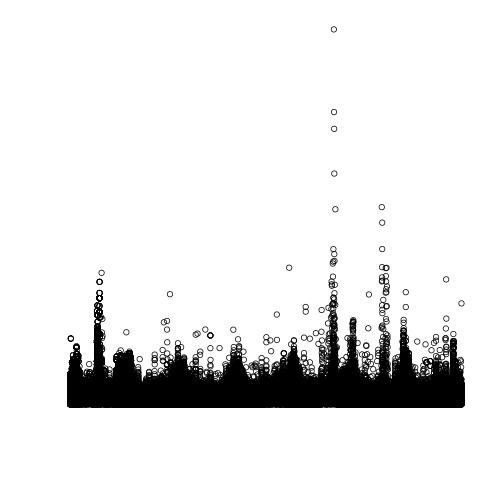
\includegraphics[width=0.77\textwidth]{Code_Outputs/ML_input_report_ML_input_PM25_Step5_part_d_de_duplicated_aves_ML_input_PM25_ObsvDate.jpg} 
\caption{\label{fig:ML_input_report_ML_input_PM25_Step5_part_d_de_duplicated_aves_ML_inputPM25_ObsvDate}PM2.5 Obs ML Inputs Time Series} 
\end{figure} 
 

\begin{figure} 
\centering  
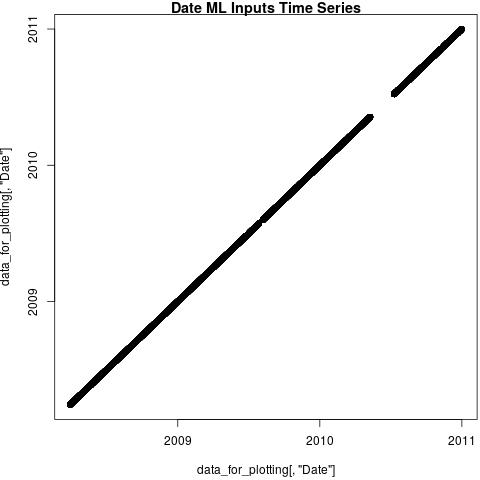
\includegraphics[width=0.77\textwidth]{Code_Outputs/ML_input_report_ML_input_PM25_Step5_part_d_de_duplicated_aves_ML_input_DatevDate.jpg} 
\caption{\label{fig:ML_input_report_ML_input_PM25_Step5_part_d_de_duplicated_aves_ML_inputDatevDate}Date ML Inputs Time Series} 
\end{figure} 
 

\begin{figure} 
\centering  
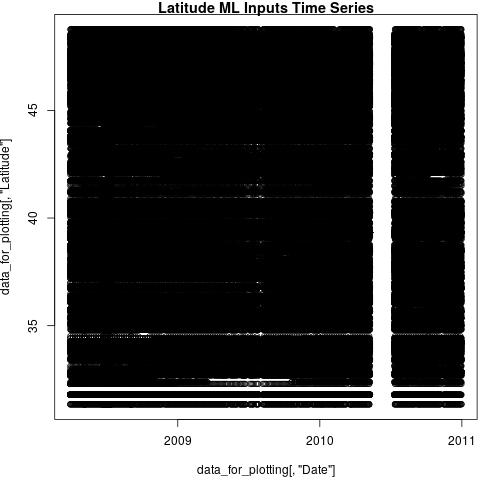
\includegraphics[width=0.77\textwidth]{Code_Outputs/ML_input_report_ML_input_PM25_Step5_part_d_de_duplicated_aves_ML_input_LatitudevDate.jpg} 
\caption{\label{fig:ML_input_report_ML_input_PM25_Step5_part_d_de_duplicated_aves_ML_inputLatitudevDate}Latitude ML Inputs Time Series} 
\end{figure} 
 

\begin{figure} 
\centering  
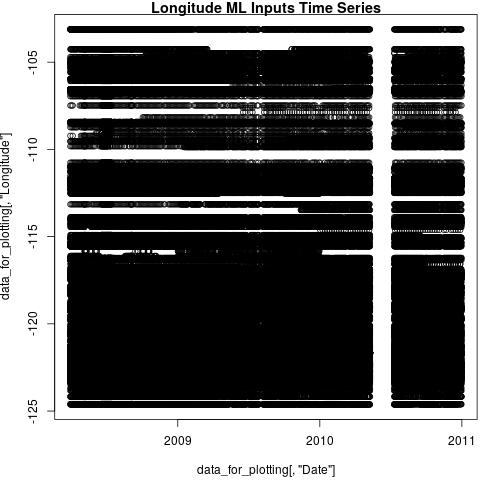
\includegraphics[width=0.77\textwidth]{Code_Outputs/ML_input_report_ML_input_PM25_Step5_part_d_de_duplicated_aves_ML_input_LongitudevDate.jpg} 
\caption{\label{fig:ML_input_report_ML_input_PM25_Step5_part_d_de_duplicated_aves_ML_inputLongitudevDate}Longitude ML Inputs Time Series} 
\end{figure} 
 

\begin{figure} 
\centering  
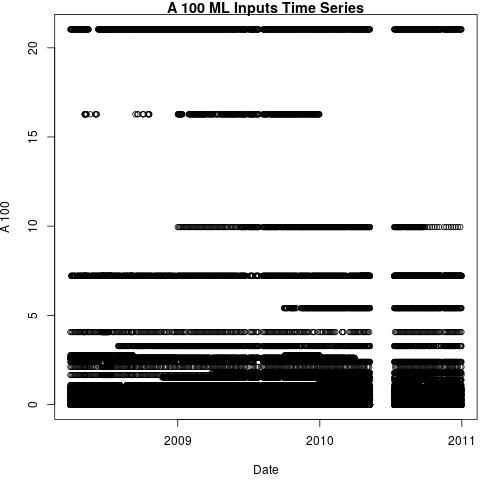
\includegraphics[width=0.77\textwidth]{Code_Outputs/ML_input_report_ML_input_PM25_Step5_part_d_de_duplicated_aves_ML_input_A_100vDate.jpg} 
\caption{\label{fig:ML_input_report_ML_input_PM25_Step5_part_d_de_duplicated_aves_ML_inputA_100vDate}A 100 ML Inputs Time Series} 
\end{figure} 
 

\begin{figure} 
\centering  
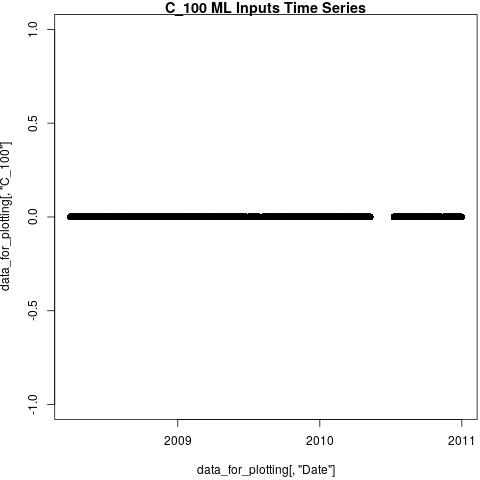
\includegraphics[width=0.77\textwidth]{Code_Outputs/ML_input_report_ML_input_PM25_Step5_part_d_de_duplicated_aves_ML_input_C_100vDate.jpg} 
\caption{\label{fig:ML_input_report_ML_input_PM25_Step5_part_d_de_duplicated_aves_ML_inputC_100vDate}C 100 ML Inputs Time Series} 
\end{figure} 
 

\begin{figure} 
\centering  
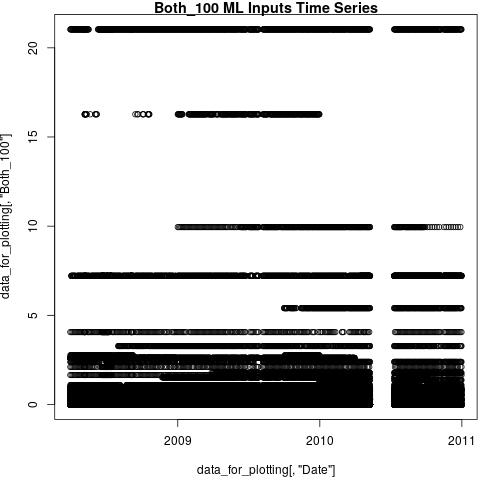
\includegraphics[width=0.77\textwidth]{Code_Outputs/ML_input_report_ML_input_PM25_Step5_part_d_de_duplicated_aves_ML_input_Both_100vDate.jpg} 
\caption{\label{fig:ML_input_report_ML_input_PM25_Step5_part_d_de_duplicated_aves_ML_inputBoth_100vDate}Both 100 ML Inputs Time Series} 
\end{figure} 
 

\begin{figure} 
\centering  
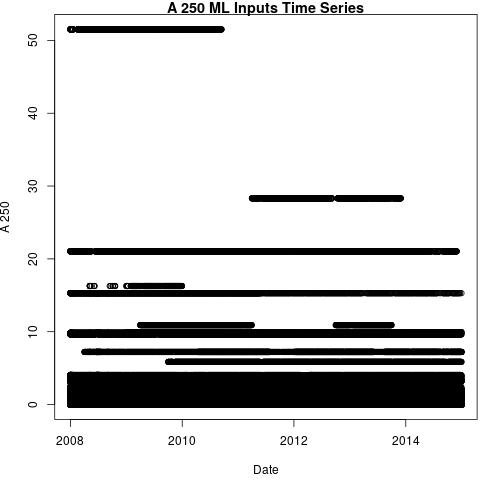
\includegraphics[width=0.77\textwidth]{Code_Outputs/ML_input_report_ML_input_PM25_Step5_part_d_de_duplicated_aves_ML_input_A_250vDate.jpg} 
\caption{\label{fig:ML_input_report_ML_input_PM25_Step5_part_d_de_duplicated_aves_ML_inputA_250vDate}A 250 ML Inputs Time Series} 
\end{figure} 
 

\begin{figure} 
\centering  
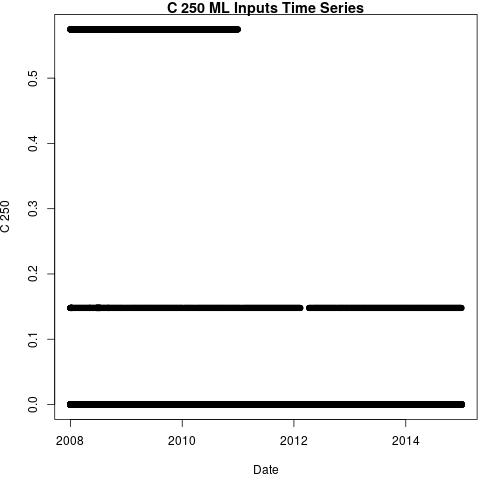
\includegraphics[width=0.77\textwidth]{Code_Outputs/ML_input_report_ML_input_PM25_Step5_part_d_de_duplicated_aves_ML_input_C_250vDate.jpg} 
\caption{\label{fig:ML_input_report_ML_input_PM25_Step5_part_d_de_duplicated_aves_ML_inputC_250vDate}C 250 ML Inputs Time Series} 
\end{figure} 
 

\clearpage 

\begin{figure} 
\centering  
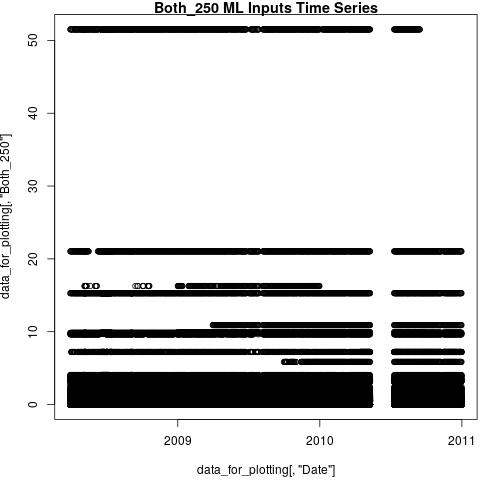
\includegraphics[width=0.77\textwidth]{Code_Outputs/ML_input_report_ML_input_PM25_Step5_part_d_de_duplicated_aves_ML_input_Both_250vDate.jpg} 
\caption{\label{fig:ML_input_report_ML_input_PM25_Step5_part_d_de_duplicated_aves_ML_inputBoth_250vDate}Both 250 ML Inputs Time Series} 
\end{figure} 
 

\begin{figure} 
\centering  
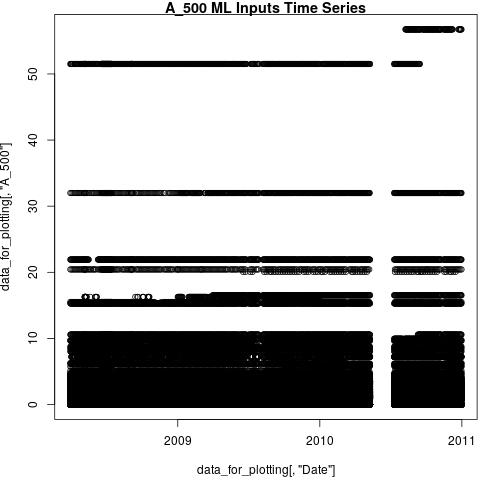
\includegraphics[width=0.77\textwidth]{Code_Outputs/ML_input_report_ML_input_PM25_Step5_part_d_de_duplicated_aves_ML_input_A_500vDate.jpg} 
\caption{\label{fig:ML_input_report_ML_input_PM25_Step5_part_d_de_duplicated_aves_ML_inputA_500vDate}A 500 ML Inputs Time Series} 
\end{figure} 
 

\begin{figure} 
\centering  
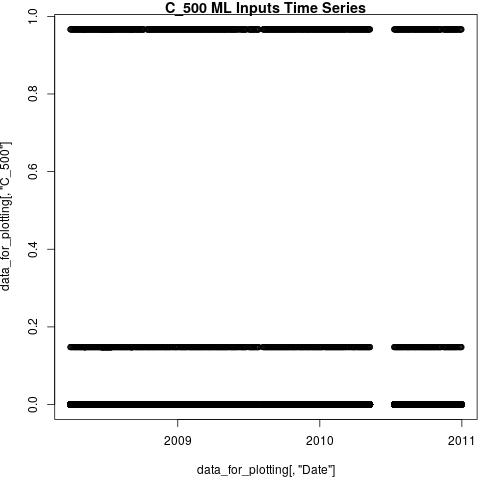
\includegraphics[width=0.77\textwidth]{Code_Outputs/ML_input_report_ML_input_PM25_Step5_part_d_de_duplicated_aves_ML_input_C_500vDate.jpg} 
\caption{\label{fig:ML_input_report_ML_input_PM25_Step5_part_d_de_duplicated_aves_ML_inputC_500vDate}C 500 ML Inputs Time Series} 
\end{figure} 
 

\begin{figure} 
\centering  
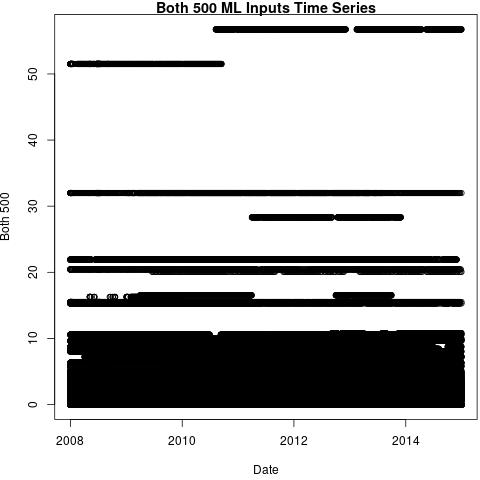
\includegraphics[width=0.77\textwidth]{Code_Outputs/ML_input_report_ML_input_PM25_Step5_part_d_de_duplicated_aves_ML_input_Both_500vDate.jpg} 
\caption{\label{fig:ML_input_report_ML_input_PM25_Step5_part_d_de_duplicated_aves_ML_inputBoth_500vDate}Both 500 ML Inputs Time Series} 
\end{figure} 
 

\begin{figure} 
\centering  
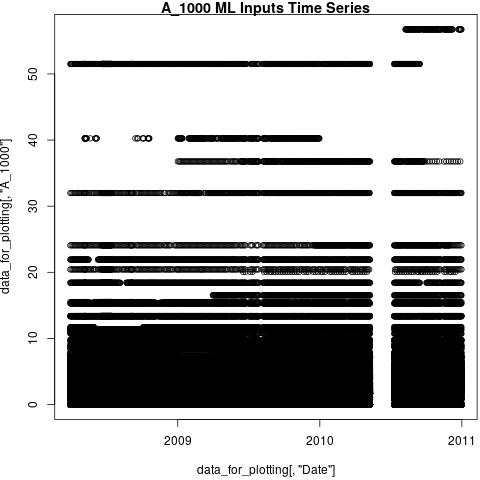
\includegraphics[width=0.77\textwidth]{Code_Outputs/ML_input_report_ML_input_PM25_Step5_part_d_de_duplicated_aves_ML_input_A_1000vDate.jpg} 
\caption{\label{fig:ML_input_report_ML_input_PM25_Step5_part_d_de_duplicated_aves_ML_inputA_1000vDate}A 1000 ML Inputs Time Series} 
\end{figure} 
 

\begin{figure} 
\centering  
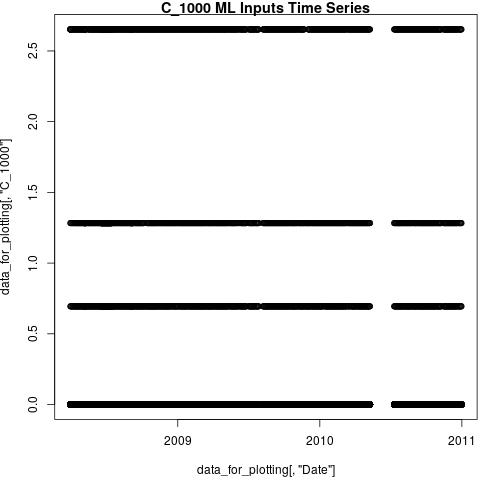
\includegraphics[width=0.77\textwidth]{Code_Outputs/ML_input_report_ML_input_PM25_Step5_part_d_de_duplicated_aves_ML_input_C_1000vDate.jpg} 
\caption{\label{fig:ML_input_report_ML_input_PM25_Step5_part_d_de_duplicated_aves_ML_inputC_1000vDate}C 1000 ML Inputs Time Series} 
\end{figure} 
 

\begin{figure} 
\centering  
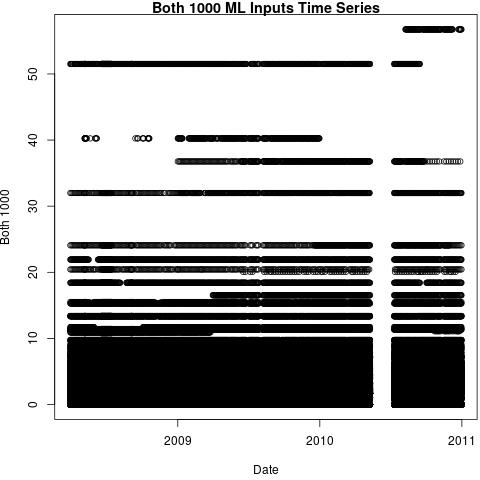
\includegraphics[width=0.77\textwidth]{Code_Outputs/ML_input_report_ML_input_PM25_Step5_part_d_de_duplicated_aves_ML_input_Both_1000vDate.jpg} 
\caption{\label{fig:ML_input_report_ML_input_PM25_Step5_part_d_de_duplicated_aves_ML_inputBoth_1000vDate}Both 1000 ML Inputs Time Series} 
\end{figure} 
 

\begin{figure} 
\centering  
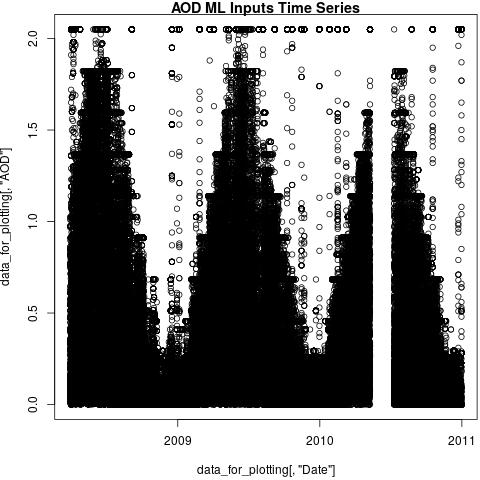
\includegraphics[width=0.77\textwidth]{Code_Outputs/ML_input_report_ML_input_PM25_Step5_part_d_de_duplicated_aves_ML_input_AODvDate.jpg} 
\caption{\label{fig:ML_input_report_ML_input_PM25_Step5_part_d_de_duplicated_aves_ML_inputAODvDate}AOD ML Inputs Time Series} 
\end{figure} 
 

\begin{figure} 
\centering  
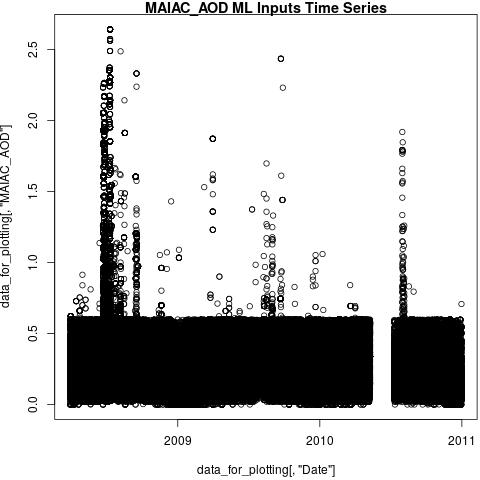
\includegraphics[width=0.77\textwidth]{Code_Outputs/ML_input_report_ML_input_PM25_Step5_part_d_de_duplicated_aves_ML_input_MAIAC_AODvDate.jpg} 
\caption{\label{fig:ML_input_report_ML_input_PM25_Step5_part_d_de_duplicated_aves_ML_inputMAIAC_AODvDate}MAIAC AOD ML Inputs Time Series} 
\end{figure} 
 

\begin{figure} 
\centering  
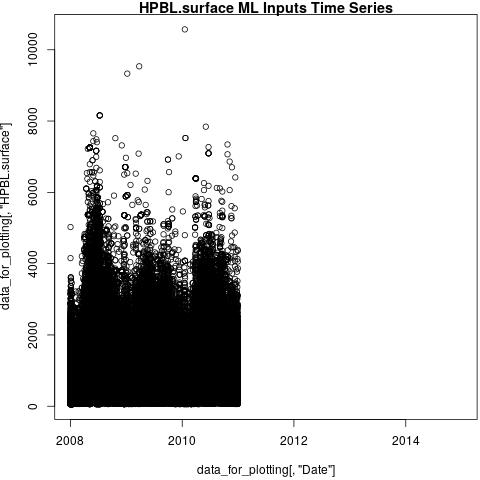
\includegraphics[width=0.77\textwidth]{Code_Outputs/ML_input_report_ML_input_PM25_Step5_part_d_de_duplicated_aves_ML_input_HPBLsurfacevDate.jpg} 
\caption{\label{fig:ML_input_report_ML_input_PM25_Step5_part_d_de_duplicated_aves_ML_inputHPBLsurfacevDate}HPBL.surface ML Inputs Time Series} 
\end{figure} 
 

\clearpage 

\begin{figure} 
\centering  
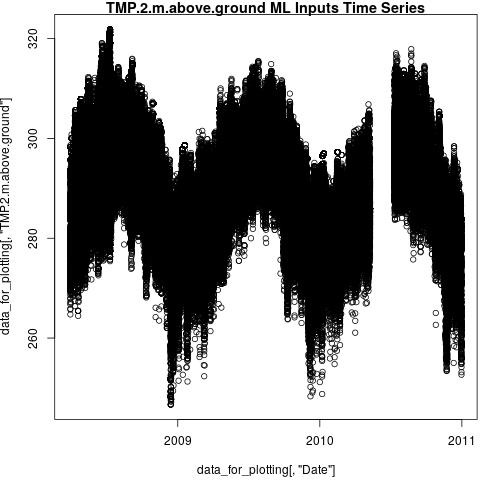
\includegraphics[width=0.77\textwidth]{Code_Outputs/ML_input_report_ML_input_PM25_Step5_part_d_de_duplicated_aves_ML_input_TMP2mabovegroundvDate.jpg} 
\caption{\label{fig:ML_input_report_ML_input_PM25_Step5_part_d_de_duplicated_aves_ML_inputTMP2mabovegroundvDate}TMP.2.m.above.ground ML Inputs Time Series} 
\end{figure} 
 

\begin{figure} 
\centering  
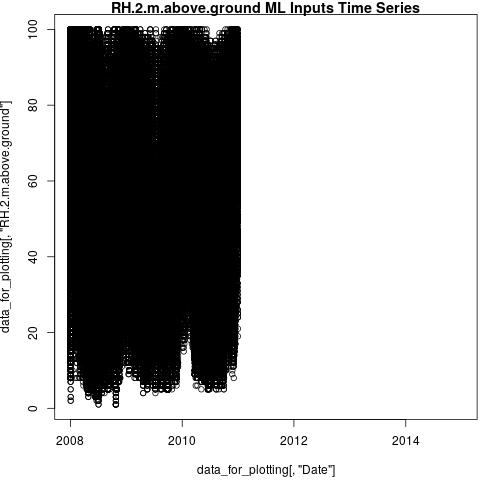
\includegraphics[width=0.77\textwidth]{Code_Outputs/ML_input_report_ML_input_PM25_Step5_part_d_de_duplicated_aves_ML_input_RH2mabovegroundvDate.jpg} 
\caption{\label{fig:ML_input_report_ML_input_PM25_Step5_part_d_de_duplicated_aves_ML_inputRH2mabovegroundvDate}RH.2.m.above.ground ML Inputs Time Series} 
\end{figure} 
 

\begin{figure} 
\centering  
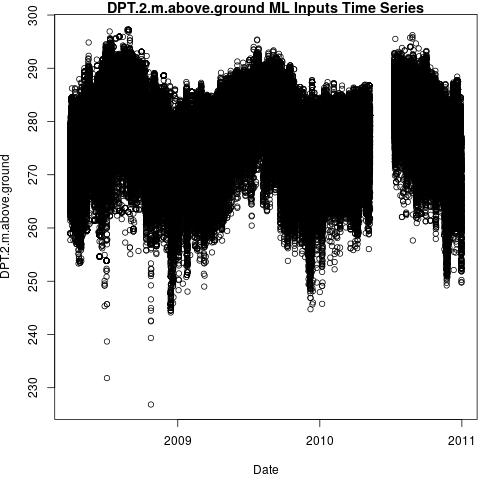
\includegraphics[width=0.77\textwidth]{Code_Outputs/ML_input_report_ML_input_PM25_Step5_part_d_de_duplicated_aves_ML_input_DPT2mabovegroundvDate.jpg} 
\caption{\label{fig:ML_input_report_ML_input_PM25_Step5_part_d_de_duplicated_aves_ML_inputDPT2mabovegroundvDate}DPT.2.m.above.ground ML Inputs Time Series} 
\end{figure} 
 

\begin{figure} 
\centering  
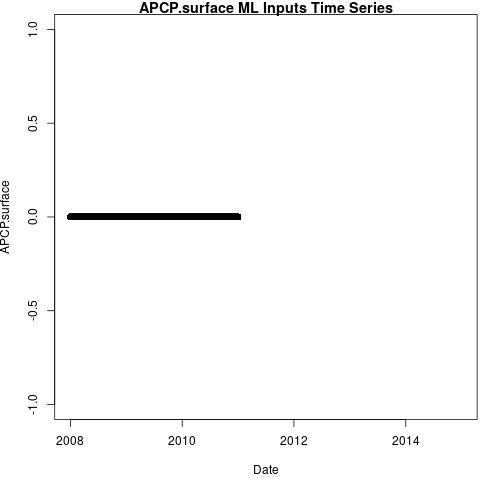
\includegraphics[width=0.77\textwidth]{Code_Outputs/ML_input_report_ML_input_PM25_Step5_part_d_de_duplicated_aves_ML_input_APCPsurfacevDate.jpg} 
\caption{\label{fig:ML_input_report_ML_input_PM25_Step5_part_d_de_duplicated_aves_ML_inputAPCPsurfacevDate}APCP.surface ML Inputs Time Series} 
\end{figure} 
 

\begin{figure} 
\centering  
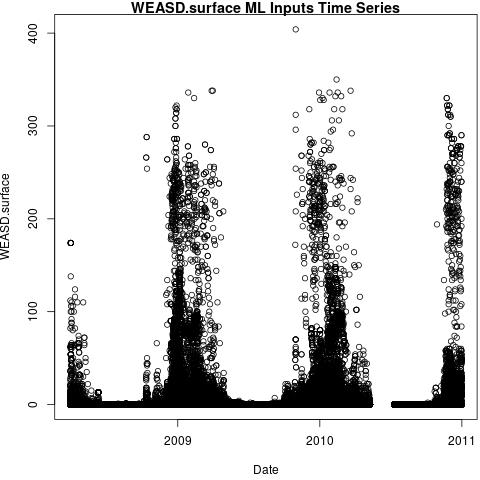
\includegraphics[width=0.77\textwidth]{Code_Outputs/ML_input_report_ML_input_PM25_Step5_part_d_de_duplicated_aves_ML_input_WEASDsurfacevDate.jpg} 
\caption{\label{fig:ML_input_report_ML_input_PM25_Step5_part_d_de_duplicated_aves_ML_inputWEASDsurfacevDate}WEASD.surface ML Inputs Time Series} 
\end{figure} 
 

\begin{figure} 
\centering  
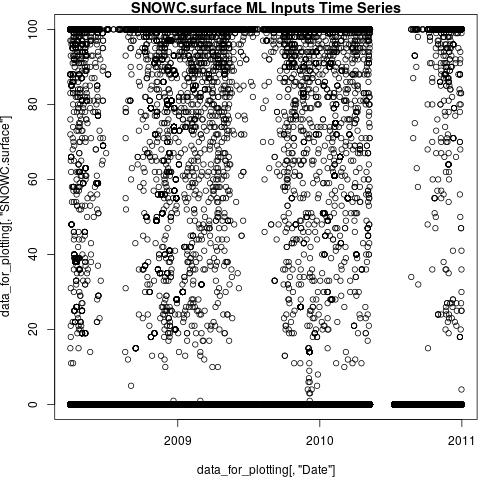
\includegraphics[width=0.77\textwidth]{Code_Outputs/ML_input_report_ML_input_PM25_Step5_part_d_de_duplicated_aves_ML_input_SNOWCsurfacevDate.jpg} 
\caption{\label{fig:ML_input_report_ML_input_PM25_Step5_part_d_de_duplicated_aves_ML_inputSNOWCsurfacevDate}SNOWC.surface ML Inputs Time Series} 
\end{figure} 
 

\begin{figure} 
\centering  
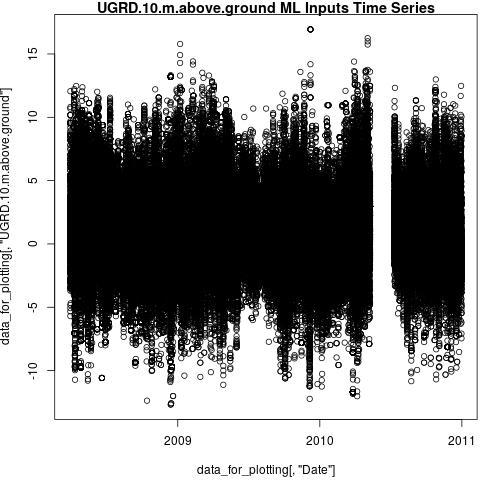
\includegraphics[width=0.77\textwidth]{Code_Outputs/ML_input_report_ML_input_PM25_Step5_part_d_de_duplicated_aves_ML_input_UGRD10mabovegroundvDate.jpg} 
\caption{\label{fig:ML_input_report_ML_input_PM25_Step5_part_d_de_duplicated_aves_ML_inputUGRD10mabovegroundvDate}UGRD.10.m.above.ground ML Inputs Time Series} 
\end{figure} 
 

\begin{figure} 
\centering  
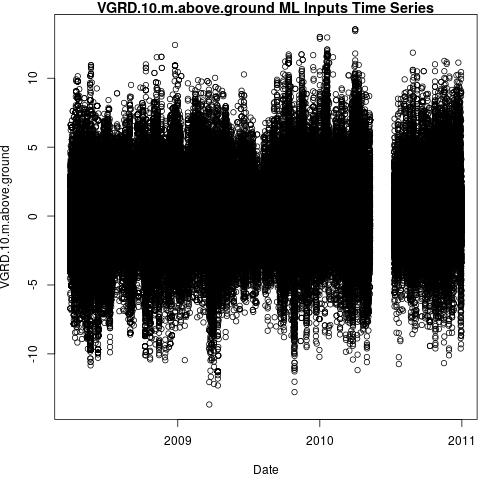
\includegraphics[width=0.77\textwidth]{Code_Outputs/ML_input_report_ML_input_PM25_Step5_part_d_de_duplicated_aves_ML_input_VGRD10mabovegroundvDate.jpg} 
\caption{\label{fig:ML_input_report_ML_input_PM25_Step5_part_d_de_duplicated_aves_ML_inputVGRD10mabovegroundvDate}VGRD.10.m.above.ground ML Inputs Time Series} 
\end{figure} 
 

\begin{figure} 
\centering  
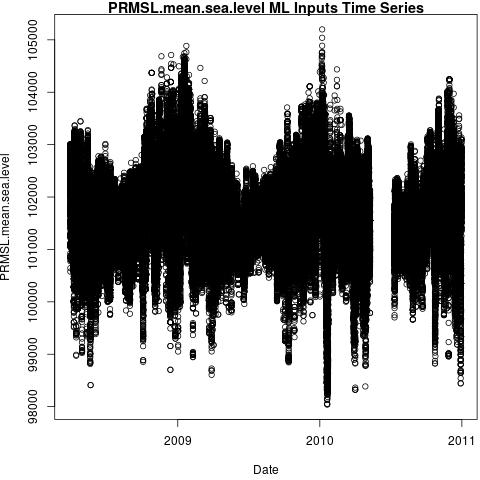
\includegraphics[width=0.77\textwidth]{Code_Outputs/ML_input_report_ML_input_PM25_Step5_part_d_de_duplicated_aves_ML_input_PRMSLmeansealevelvDate.jpg} 
\caption{\label{fig:ML_input_report_ML_input_PM25_Step5_part_d_de_duplicated_aves_ML_inputPRMSLmeansealevelvDate}PRMSL.mean.sea.level ML Inputs Time Series} 
\end{figure} 
 

\begin{figure} 
\centering  
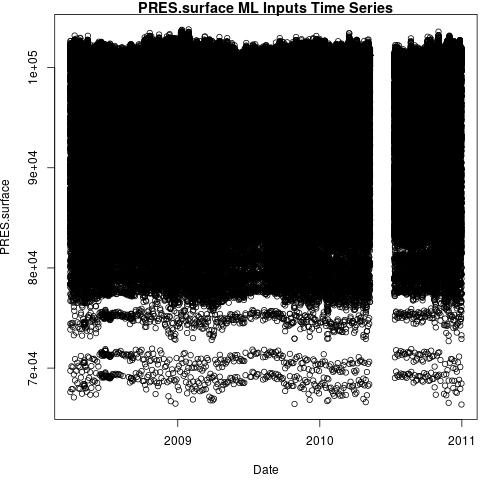
\includegraphics[width=0.77\textwidth]{Code_Outputs/ML_input_report_ML_input_PM25_Step5_part_d_de_duplicated_aves_ML_input_PRESsurfacevDate.jpg} 
\caption{\label{fig:ML_input_report_ML_input_PM25_Step5_part_d_de_duplicated_aves_ML_inputPRESsurfacevDate}PRES.surface ML Inputs Time Series} 
\end{figure} 
 

\clearpage 

\begin{figure} 
\centering  
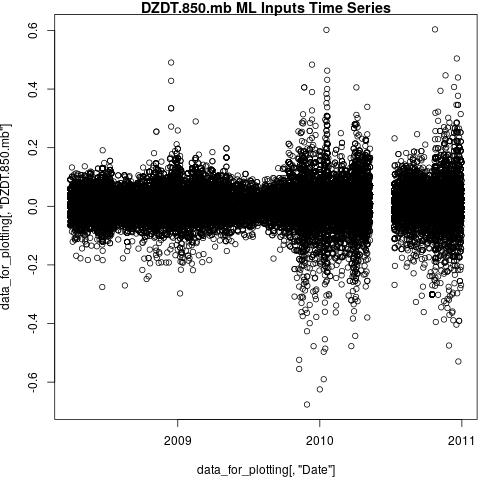
\includegraphics[width=0.77\textwidth]{Code_Outputs/ML_input_report_ML_input_PM25_Step5_part_d_de_duplicated_aves_ML_input_DZDT850mbvDate.jpg} 
\caption{\label{fig:ML_input_report_ML_input_PM25_Step5_part_d_de_duplicated_aves_ML_inputDZDT850mbvDate}DZDT.850.mb ML Inputs Time Series} 
\end{figure} 
 

\begin{figure} 
\centering  
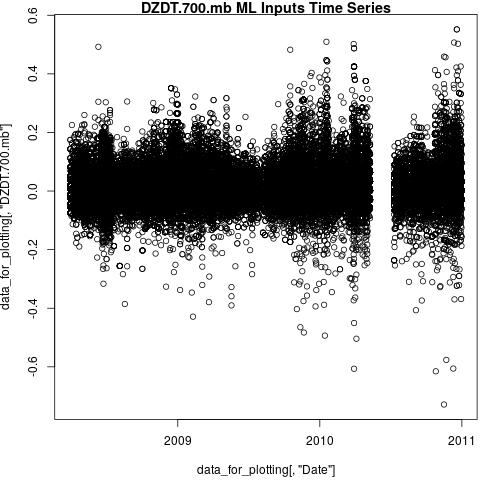
\includegraphics[width=0.77\textwidth]{Code_Outputs/ML_input_report_ML_input_PM25_Step5_part_d_de_duplicated_aves_ML_input_DZDT700mbvDate.jpg} 
\caption{\label{fig:ML_input_report_ML_input_PM25_Step5_part_d_de_duplicated_aves_ML_inputDZDT700mbvDate}DZDT.700.mb ML Inputs Time Series} 
\end{figure} 
 

\begin{figure} 
\centering  
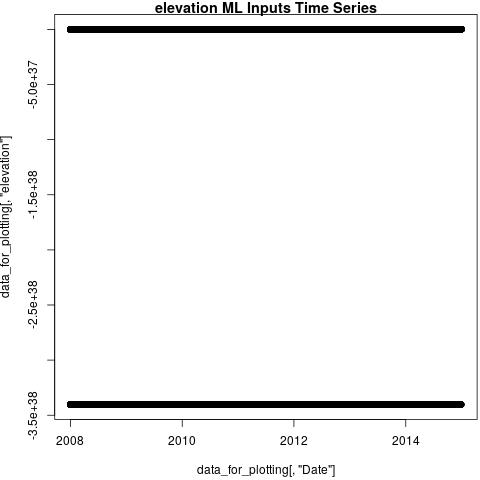
\includegraphics[width=0.77\textwidth]{Code_Outputs/ML_input_report_ML_input_PM25_Step5_part_d_de_duplicated_aves_ML_input_elevationvDate.jpg} 
\caption{\label{fig:ML_input_report_ML_input_PM25_Step5_part_d_de_duplicated_aves_ML_inputelevationvDate}elevation ML Inputs Time Series} 
\end{figure} 
 

\begin{figure} 
\centering  
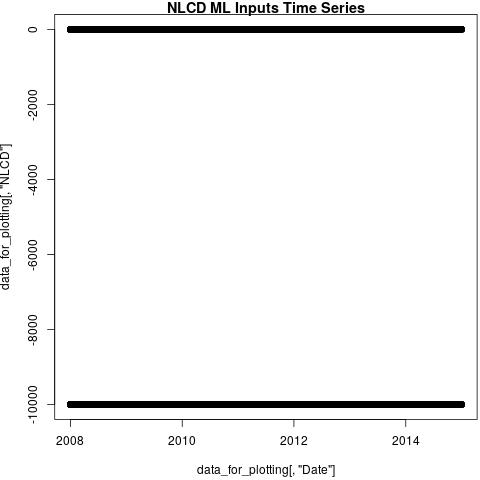
\includegraphics[width=0.77\textwidth]{Code_Outputs/ML_input_report_ML_input_PM25_Step5_part_d_de_duplicated_aves_ML_input_NLCDvDate.jpg} 
\caption{\label{fig:ML_input_report_ML_input_PM25_Step5_part_d_de_duplicated_aves_ML_inputNLCDvDate}NLCD ML Inputs Time Series} 
\end{figure} 
 


\clearpage

\subsection{ML Inputs Map subset of days Images} 
 

\begin{figure} 
\centering  
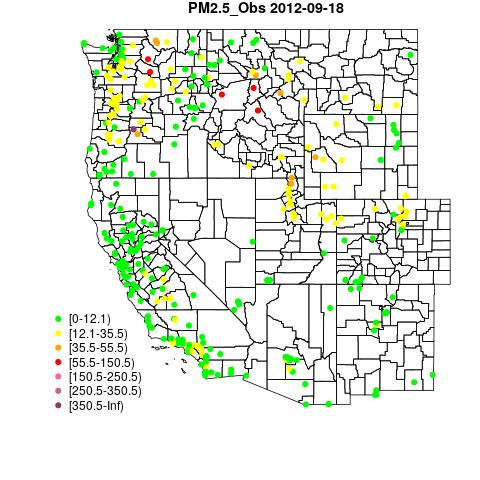
\includegraphics[width=0.77\textwidth]{Code_Outputs/ML_input_report_ML_input_PM25_Step5_part_d_de_duplicated_aves_ML_input_MapObsPM25_Obs2012-09-18.jpg} 
\caption{\label{fig:ML_input_report_ML_input_PM25_Step5_part_d_de_duplicated_aves_ML_inputMapObsPM25_Obs2012-09-18}PM2.5-Obs 2012-09-18} 
\end{figure} 
 

\begin{figure} 
\centering  
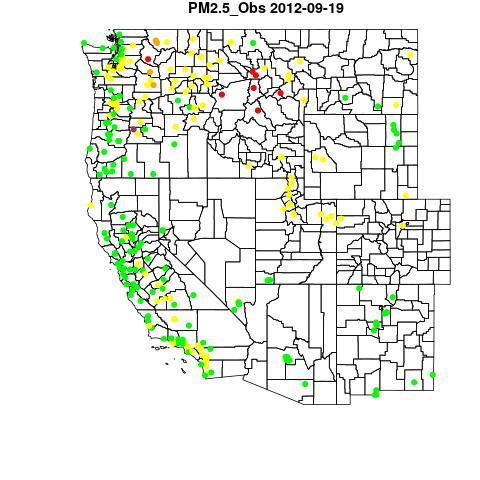
\includegraphics[width=0.77\textwidth]{Code_Outputs/ML_input_report_ML_input_PM25_Step5_part_d_de_duplicated_aves_ML_input_MapObsPM25_Obs2012-09-19.jpg} 
\caption{\label{fig:ML_input_report_ML_input_PM25_Step5_part_d_de_duplicated_aves_ML_inputMapObsPM25_Obs2012-09-19}PM2.5-Obs 2012-09-19} 
\end{figure} 
 

\begin{figure} 
\centering  
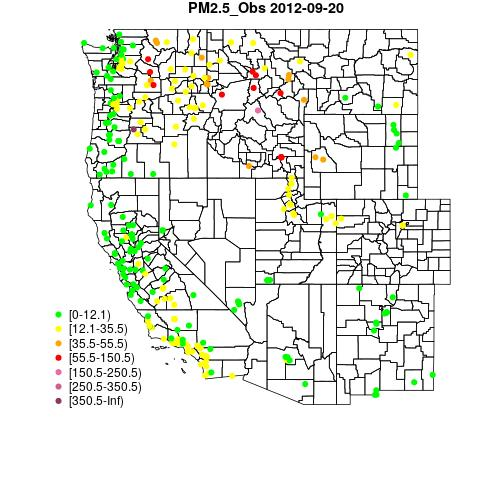
\includegraphics[width=0.77\textwidth]{Code_Outputs/ML_input_report_ML_input_PM25_Step5_part_d_de_duplicated_aves_ML_input_MapObsPM25_Obs2012-09-20.jpg} 
\caption{\label{fig:ML_input_report_ML_input_PM25_Step5_part_d_de_duplicated_aves_ML_inputMapObsPM25_Obs2012-09-20}PM2.5-Obs 2012-09-20} 
\end{figure} 
 

\begin{figure} 
\centering  
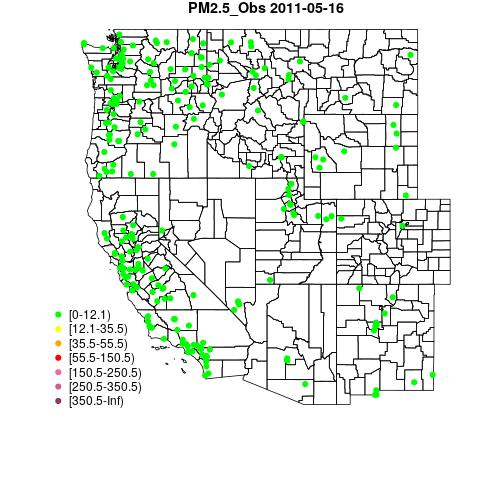
\includegraphics[width=0.77\textwidth]{Code_Outputs/ML_input_report_ML_input_PM25_Step5_part_d_de_duplicated_aves_ML_input_MapObsPM25_Obs2011-05-16.jpg} 
\caption{\label{fig:ML_input_report_ML_input_PM25_Step5_part_d_de_duplicated_aves_ML_inputMapObsPM25_Obs2011-05-16}PM2.5-Obs 2011-05-16} 
\end{figure} 
 

\begin{figure} 
\centering  
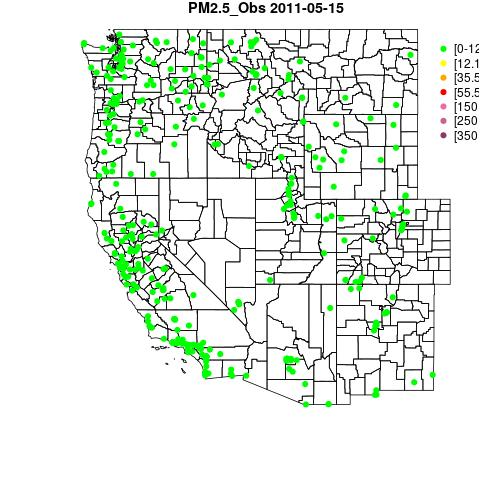
\includegraphics[width=0.77\textwidth]{Code_Outputs/ML_input_report_ML_input_PM25_Step5_part_d_de_duplicated_aves_ML_input_MapObsPM25_Obs2011-05-15.jpg} 
\caption{\label{fig:ML_input_report_ML_input_PM25_Step5_part_d_de_duplicated_aves_ML_inputMapObsPM25_Obs2011-05-15}PM2.5-Obs 2011-05-15} 
\end{figure} 
 

\begin{figure} 
\centering  
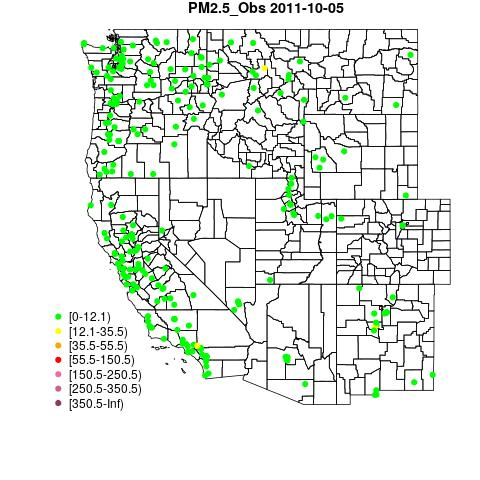
\includegraphics[width=0.77\textwidth]{Code_Outputs/ML_input_report_ML_input_PM25_Step5_part_d_de_duplicated_aves_ML_input_MapObsPM25_Obs2011-10-05.jpg} 
\caption{\label{fig:ML_input_report_ML_input_PM25_Step5_part_d_de_duplicated_aves_ML_inputMapObsPM25_Obs2011-10-05}PM2.5-Obs 2011-10-05} 
\end{figure} 
 

\begin{figure} 
\centering  
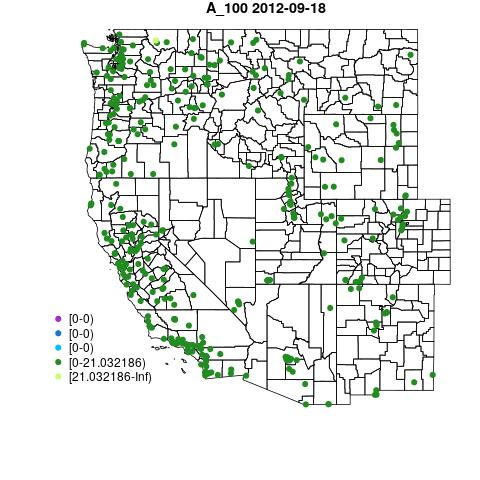
\includegraphics[width=0.77\textwidth]{Code_Outputs/ML_input_report_ML_input_PM25_Step5_part_d_de_duplicated_aves_ML_input_MapObsA_1002012-09-18.jpg} 
\caption{\label{fig:ML_input_report_ML_input_PM25_Step5_part_d_de_duplicated_aves_ML_inputMapObsA_1002012-09-18}A-100 2012-09-18} 
\end{figure} 
 

\begin{figure} 
\centering  
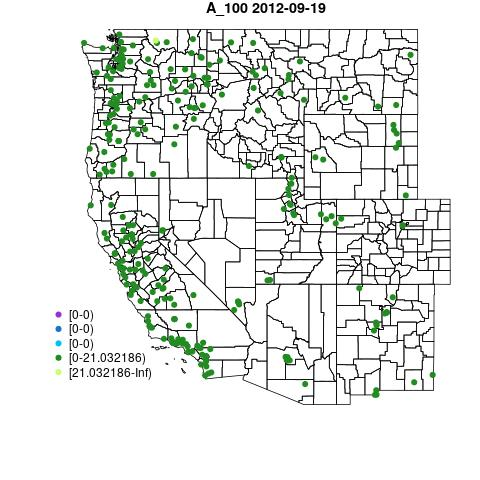
\includegraphics[width=0.77\textwidth]{Code_Outputs/ML_input_report_ML_input_PM25_Step5_part_d_de_duplicated_aves_ML_input_MapObsA_1002012-09-19.jpg} 
\caption{\label{fig:ML_input_report_ML_input_PM25_Step5_part_d_de_duplicated_aves_ML_inputMapObsA_1002012-09-19}A-100 2012-09-19} 
\end{figure} 
 

\begin{figure} 
\centering  
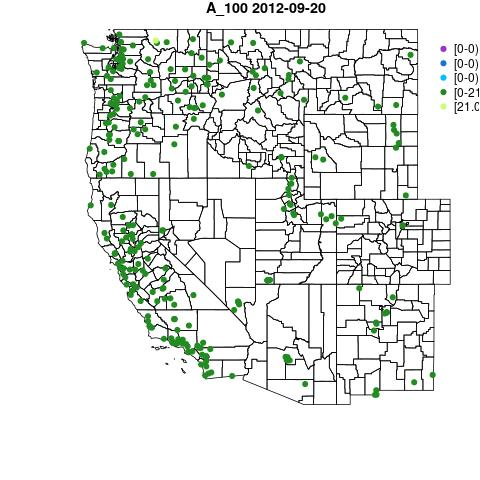
\includegraphics[width=0.77\textwidth]{Code_Outputs/ML_input_report_ML_input_PM25_Step5_part_d_de_duplicated_aves_ML_input_MapObsA_1002012-09-20.jpg} 
\caption{\label{fig:ML_input_report_ML_input_PM25_Step5_part_d_de_duplicated_aves_ML_inputMapObsA_1002012-09-20}A-100 2012-09-20} 
\end{figure} 
 

\clearpage 

\begin{figure} 
\centering  
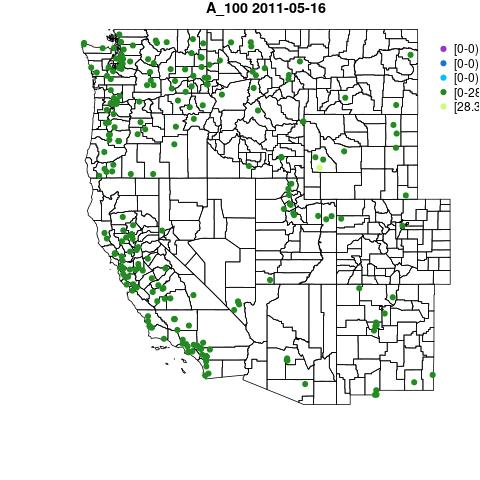
\includegraphics[width=0.77\textwidth]{Code_Outputs/ML_input_report_ML_input_PM25_Step5_part_d_de_duplicated_aves_ML_input_MapObsA_1002011-05-16.jpg} 
\caption{\label{fig:ML_input_report_ML_input_PM25_Step5_part_d_de_duplicated_aves_ML_inputMapObsA_1002011-05-16}A-100 2011-05-16} 
\end{figure} 
 

\begin{figure} 
\centering  
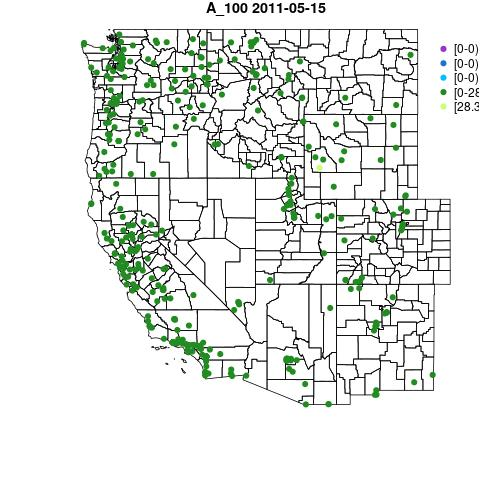
\includegraphics[width=0.77\textwidth]{Code_Outputs/ML_input_report_ML_input_PM25_Step5_part_d_de_duplicated_aves_ML_input_MapObsA_1002011-05-15.jpg} 
\caption{\label{fig:ML_input_report_ML_input_PM25_Step5_part_d_de_duplicated_aves_ML_inputMapObsA_1002011-05-15}A-100 2011-05-15} 
\end{figure} 
 

\begin{figure} 
\centering  
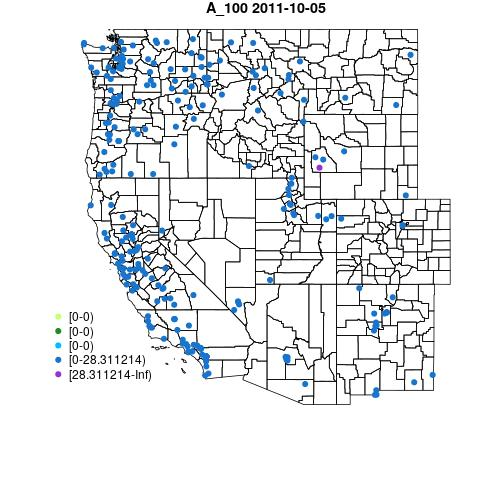
\includegraphics[width=0.77\textwidth]{Code_Outputs/ML_input_report_ML_input_PM25_Step5_part_d_de_duplicated_aves_ML_input_MapObsA_1002011-10-05.jpg} 
\caption{\label{fig:ML_input_report_ML_input_PM25_Step5_part_d_de_duplicated_aves_ML_inputMapObsA_1002011-10-05}A-100 2011-10-05} 
\end{figure} 
 

\begin{figure} 
\centering  
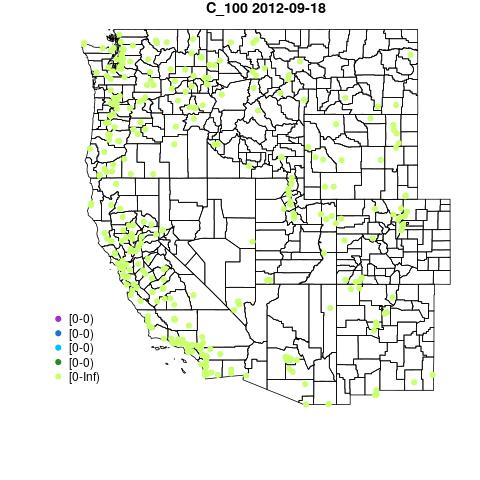
\includegraphics[width=0.77\textwidth]{Code_Outputs/ML_input_report_ML_input_PM25_Step5_part_d_de_duplicated_aves_ML_input_MapObsC_1002012-09-18.jpg} 
\caption{\label{fig:ML_input_report_ML_input_PM25_Step5_part_d_de_duplicated_aves_ML_inputMapObsC_1002012-09-18}C-100 2012-09-18} 
\end{figure} 
 

\begin{figure} 
\centering  
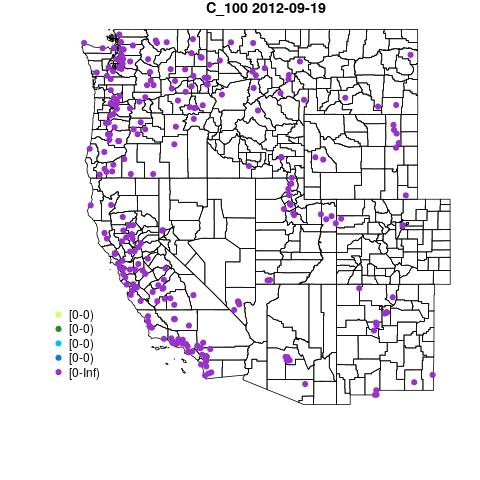
\includegraphics[width=0.77\textwidth]{Code_Outputs/ML_input_report_ML_input_PM25_Step5_part_d_de_duplicated_aves_ML_input_MapObsC_1002012-09-19.jpg} 
\caption{\label{fig:ML_input_report_ML_input_PM25_Step5_part_d_de_duplicated_aves_ML_inputMapObsC_1002012-09-19}C-100 2012-09-19} 
\end{figure} 
 

\begin{figure} 
\centering  
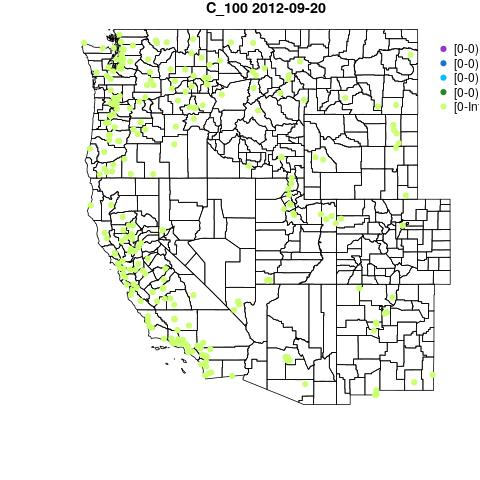
\includegraphics[width=0.77\textwidth]{Code_Outputs/ML_input_report_ML_input_PM25_Step5_part_d_de_duplicated_aves_ML_input_MapObsC_1002012-09-20.jpg} 
\caption{\label{fig:ML_input_report_ML_input_PM25_Step5_part_d_de_duplicated_aves_ML_inputMapObsC_1002012-09-20}C-100 2012-09-20} 
\end{figure} 
 

\begin{figure} 
\centering  
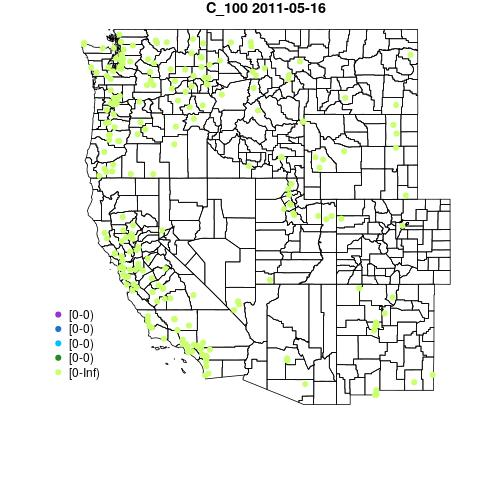
\includegraphics[width=0.77\textwidth]{Code_Outputs/ML_input_report_ML_input_PM25_Step5_part_d_de_duplicated_aves_ML_input_MapObsC_1002011-05-16.jpg} 
\caption{\label{fig:ML_input_report_ML_input_PM25_Step5_part_d_de_duplicated_aves_ML_inputMapObsC_1002011-05-16}C-100 2011-05-16} 
\end{figure} 
 

\begin{figure} 
\centering  
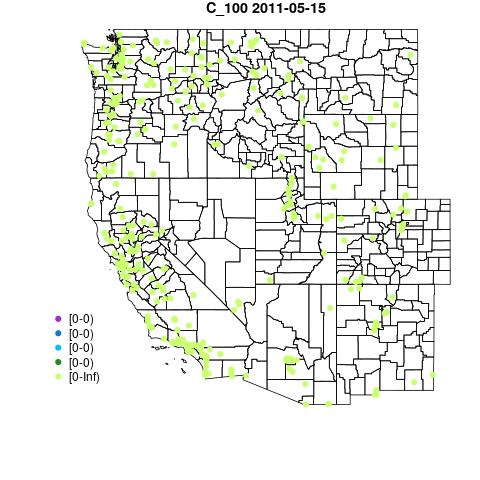
\includegraphics[width=0.77\textwidth]{Code_Outputs/ML_input_report_ML_input_PM25_Step5_part_d_de_duplicated_aves_ML_input_MapObsC_1002011-05-15.jpg} 
\caption{\label{fig:ML_input_report_ML_input_PM25_Step5_part_d_de_duplicated_aves_ML_inputMapObsC_1002011-05-15}C-100 2011-05-15} 
\end{figure} 
 

\begin{figure} 
\centering  
\includegraphics[width=0.77\textwidth]{Code_Outputs/ML_input_report_ML_input_PM25_Step5_part_d_de_duplicated_aves_ML_input_MapObsC_1002011-10-05.jpg} 
\caption{\label{fig:ML_input_report_ML_input_PM25_Step5_part_d_de_duplicated_aves_ML_inputMapObsC_1002011-10-05}C-100 2011-10-05} 
\end{figure} 
 

\begin{figure} 
\centering  
\includegraphics[width=0.77\textwidth]{Code_Outputs/ML_input_report_ML_input_PM25_Step5_part_d_de_duplicated_aves_ML_input_MapObsBoth_1002012-09-18.jpg} 
\caption{\label{fig:ML_input_report_ML_input_PM25_Step5_part_d_de_duplicated_aves_ML_inputMapObsBoth_1002012-09-18}Both-100 2012-09-18} 
\end{figure} 
 

\clearpage 

\begin{figure} 
\centering  
\includegraphics[width=0.77\textwidth]{Code_Outputs/ML_input_report_ML_input_PM25_Step5_part_d_de_duplicated_aves_ML_input_MapObsBoth_1002012-09-19.jpg} 
\caption{\label{fig:ML_input_report_ML_input_PM25_Step5_part_d_de_duplicated_aves_ML_inputMapObsBoth_1002012-09-19}Both-100 2012-09-19} 
\end{figure} 
 

\begin{figure} 
\centering  
\includegraphics[width=0.77\textwidth]{Code_Outputs/ML_input_report_ML_input_PM25_Step5_part_d_de_duplicated_aves_ML_input_MapObsBoth_1002012-09-20.jpg} 
\caption{\label{fig:ML_input_report_ML_input_PM25_Step5_part_d_de_duplicated_aves_ML_inputMapObsBoth_1002012-09-20}Both-100 2012-09-20} 
\end{figure} 
 

\begin{figure} 
\centering  
\includegraphics[width=0.77\textwidth]{Code_Outputs/ML_input_report_ML_input_PM25_Step5_part_d_de_duplicated_aves_ML_input_MapObsBoth_1002011-05-16.jpg} 
\caption{\label{fig:ML_input_report_ML_input_PM25_Step5_part_d_de_duplicated_aves_ML_inputMapObsBoth_1002011-05-16}Both-100 2011-05-16} 
\end{figure} 
 

\begin{figure} 
\centering  
\includegraphics[width=0.77\textwidth]{Code_Outputs/ML_input_report_ML_input_PM25_Step5_part_d_de_duplicated_aves_ML_input_MapObsBoth_1002011-05-15.jpg} 
\caption{\label{fig:ML_input_report_ML_input_PM25_Step5_part_d_de_duplicated_aves_ML_inputMapObsBoth_1002011-05-15}Both-100 2011-05-15} 
\end{figure} 
 

\begin{figure} 
\centering  
\includegraphics[width=0.77\textwidth]{Code_Outputs/ML_input_report_ML_input_PM25_Step5_part_d_de_duplicated_aves_ML_input_MapObsBoth_1002011-10-05.jpg} 
\caption{\label{fig:ML_input_report_ML_input_PM25_Step5_part_d_de_duplicated_aves_ML_inputMapObsBoth_1002011-10-05}Both-100 2011-10-05} 
\end{figure} 
 

\begin{figure} 
\centering  
\includegraphics[width=0.77\textwidth]{Code_Outputs/ML_input_report_ML_input_PM25_Step5_part_d_de_duplicated_aves_ML_input_MapObsA_2502012-09-18.jpg} 
\caption{\label{fig:ML_input_report_ML_input_PM25_Step5_part_d_de_duplicated_aves_ML_inputMapObsA_2502012-09-18}A-250 2012-09-18} 
\end{figure} 
 

\begin{figure} 
\centering  
\includegraphics[width=0.77\textwidth]{Code_Outputs/ML_input_report_ML_input_PM25_Step5_part_d_de_duplicated_aves_ML_input_MapObsA_2502012-09-19.jpg} 
\caption{\label{fig:ML_input_report_ML_input_PM25_Step5_part_d_de_duplicated_aves_ML_inputMapObsA_2502012-09-19}A-250 2012-09-19} 
\end{figure} 
 

\begin{figure} 
\centering  
\includegraphics[width=0.77\textwidth]{Code_Outputs/ML_input_report_ML_input_PM25_Step5_part_d_de_duplicated_aves_ML_input_MapObsA_2502012-09-20.jpg} 
\caption{\label{fig:ML_input_report_ML_input_PM25_Step5_part_d_de_duplicated_aves_ML_inputMapObsA_2502012-09-20}A-250 2012-09-20} 
\end{figure} 
 

\begin{figure} 
\centering  
\includegraphics[width=0.77\textwidth]{Code_Outputs/ML_input_report_ML_input_PM25_Step5_part_d_de_duplicated_aves_ML_input_MapObsA_2502011-05-16.jpg} 
\caption{\label{fig:ML_input_report_ML_input_PM25_Step5_part_d_de_duplicated_aves_ML_inputMapObsA_2502011-05-16}A-250 2011-05-16} 
\end{figure} 
 

\begin{figure} 
\centering  
\includegraphics[width=0.77\textwidth]{Code_Outputs/ML_input_report_ML_input_PM25_Step5_part_d_de_duplicated_aves_ML_input_MapObsA_2502011-05-15.jpg} 
\caption{\label{fig:ML_input_report_ML_input_PM25_Step5_part_d_de_duplicated_aves_ML_inputMapObsA_2502011-05-15}A-250 2011-05-15} 
\end{figure} 
 

\clearpage 

\begin{figure} 
\centering  
\includegraphics[width=0.77\textwidth]{Code_Outputs/ML_input_report_ML_input_PM25_Step5_part_d_de_duplicated_aves_ML_input_MapObsA_2502011-10-05.jpg} 
\caption{\label{fig:ML_input_report_ML_input_PM25_Step5_part_d_de_duplicated_aves_ML_inputMapObsA_2502011-10-05}A-250 2011-10-05} 
\end{figure} 
 

\begin{figure} 
\centering  
\includegraphics[width=0.77\textwidth]{Code_Outputs/ML_input_report_ML_input_PM25_Step5_part_d_de_duplicated_aves_ML_input_MapObsC_2502012-09-18.jpg} 
\caption{\label{fig:ML_input_report_ML_input_PM25_Step5_part_d_de_duplicated_aves_ML_inputMapObsC_2502012-09-18}C-250 2012-09-18} 
\end{figure} 
 

\begin{figure} 
\centering  
\includegraphics[width=0.77\textwidth]{Code_Outputs/ML_input_report_ML_input_PM25_Step5_part_d_de_duplicated_aves_ML_input_MapObsC_2502012-09-19.jpg} 
\caption{\label{fig:ML_input_report_ML_input_PM25_Step5_part_d_de_duplicated_aves_ML_inputMapObsC_2502012-09-19}C-250 2012-09-19} 
\end{figure} 
 

\begin{figure} 
\centering  
\includegraphics[width=0.77\textwidth]{Code_Outputs/ML_input_report_ML_input_PM25_Step5_part_d_de_duplicated_aves_ML_input_MapObsC_2502012-09-20.jpg} 
\caption{\label{fig:ML_input_report_ML_input_PM25_Step5_part_d_de_duplicated_aves_ML_inputMapObsC_2502012-09-20}C-250 2012-09-20} 
\end{figure} 
 

\begin{figure} 
\centering  
\includegraphics[width=0.77\textwidth]{Code_Outputs/ML_input_report_ML_input_PM25_Step5_part_d_de_duplicated_aves_ML_input_MapObsC_2502011-05-16.jpg} 
\caption{\label{fig:ML_input_report_ML_input_PM25_Step5_part_d_de_duplicated_aves_ML_inputMapObsC_2502011-05-16}C-250 2011-05-16} 
\end{figure} 
 

\begin{figure} 
\centering  
\includegraphics[width=0.77\textwidth]{Code_Outputs/ML_input_report_ML_input_PM25_Step5_part_d_de_duplicated_aves_ML_input_MapObsC_2502011-05-15.jpg} 
\caption{\label{fig:ML_input_report_ML_input_PM25_Step5_part_d_de_duplicated_aves_ML_inputMapObsC_2502011-05-15}C-250 2011-05-15} 
\end{figure} 
 

\begin{figure} 
\centering  
\includegraphics[width=0.77\textwidth]{Code_Outputs/ML_input_report_ML_input_PM25_Step5_part_d_de_duplicated_aves_ML_input_MapObsC_2502011-10-05.jpg} 
\caption{\label{fig:ML_input_report_ML_input_PM25_Step5_part_d_de_duplicated_aves_ML_inputMapObsC_2502011-10-05}C-250 2011-10-05} 
\end{figure} 
 

\begin{figure} 
\centering  
\includegraphics[width=0.77\textwidth]{Code_Outputs/ML_input_report_ML_input_PM25_Step5_part_d_de_duplicated_aves_ML_input_MapObsBoth_2502012-09-18.jpg} 
\caption{\label{fig:ML_input_report_ML_input_PM25_Step5_part_d_de_duplicated_aves_ML_inputMapObsBoth_2502012-09-18}Both-250 2012-09-18} 
\end{figure} 
 

\begin{figure} 
\centering  
\includegraphics[width=0.77\textwidth]{Code_Outputs/ML_input_report_ML_input_PM25_Step5_part_d_de_duplicated_aves_ML_input_MapObsBoth_2502012-09-19.jpg} 
\caption{\label{fig:ML_input_report_ML_input_PM25_Step5_part_d_de_duplicated_aves_ML_inputMapObsBoth_2502012-09-19}Both-250 2012-09-19} 
\end{figure} 
 

\begin{figure} 
\centering  
\includegraphics[width=0.77\textwidth]{Code_Outputs/ML_input_report_ML_input_PM25_Step5_part_d_de_duplicated_aves_ML_input_MapObsBoth_2502012-09-20.jpg} 
\caption{\label{fig:ML_input_report_ML_input_PM25_Step5_part_d_de_duplicated_aves_ML_inputMapObsBoth_2502012-09-20}Both-250 2012-09-20} 
\end{figure} 
 

\clearpage 

\begin{figure} 
\centering  
\includegraphics[width=0.77\textwidth]{Code_Outputs/ML_input_report_ML_input_PM25_Step5_part_d_de_duplicated_aves_ML_input_MapObsBoth_2502011-05-16.jpg} 
\caption{\label{fig:ML_input_report_ML_input_PM25_Step5_part_d_de_duplicated_aves_ML_inputMapObsBoth_2502011-05-16}Both-250 2011-05-16} 
\end{figure} 
 

\begin{figure} 
\centering  
\includegraphics[width=0.77\textwidth]{Code_Outputs/ML_input_report_ML_input_PM25_Step5_part_d_de_duplicated_aves_ML_input_MapObsBoth_2502011-05-15.jpg} 
\caption{\label{fig:ML_input_report_ML_input_PM25_Step5_part_d_de_duplicated_aves_ML_inputMapObsBoth_2502011-05-15}Both-250 2011-05-15} 
\end{figure} 
 

\begin{figure} 
\centering  
\includegraphics[width=0.77\textwidth]{Code_Outputs/ML_input_report_ML_input_PM25_Step5_part_d_de_duplicated_aves_ML_input_MapObsBoth_2502011-10-05.jpg} 
\caption{\label{fig:ML_input_report_ML_input_PM25_Step5_part_d_de_duplicated_aves_ML_inputMapObsBoth_2502011-10-05}Both-250 2011-10-05} 
\end{figure} 
 

\begin{figure} 
\centering  
\includegraphics[width=0.77\textwidth]{Code_Outputs/ML_input_report_ML_input_PM25_Step5_part_d_de_duplicated_aves_ML_input_MapObsA_5002012-09-18.jpg} 
\caption{\label{fig:ML_input_report_ML_input_PM25_Step5_part_d_de_duplicated_aves_ML_inputMapObsA_5002012-09-18}A-500 2012-09-18} 
\end{figure} 
 

\begin{figure} 
\centering  
\includegraphics[width=0.77\textwidth]{Code_Outputs/ML_input_report_ML_input_PM25_Step5_part_d_de_duplicated_aves_ML_input_MapObsA_5002012-09-19.jpg} 
\caption{\label{fig:ML_input_report_ML_input_PM25_Step5_part_d_de_duplicated_aves_ML_inputMapObsA_5002012-09-19}A-500 2012-09-19} 
\end{figure} 
 

\begin{figure} 
\centering  
\includegraphics[width=0.77\textwidth]{Code_Outputs/ML_input_report_ML_input_PM25_Step5_part_d_de_duplicated_aves_ML_input_MapObsA_5002012-09-20.jpg} 
\caption{\label{fig:ML_input_report_ML_input_PM25_Step5_part_d_de_duplicated_aves_ML_inputMapObsA_5002012-09-20}A-500 2012-09-20} 
\end{figure} 
 

\begin{figure} 
\centering  
\includegraphics[width=0.77\textwidth]{Code_Outputs/ML_input_report_ML_input_PM25_Step5_part_d_de_duplicated_aves_ML_input_MapObsA_5002011-05-16.jpg} 
\caption{\label{fig:ML_input_report_ML_input_PM25_Step5_part_d_de_duplicated_aves_ML_inputMapObsA_5002011-05-16}A-500 2011-05-16} 
\end{figure} 
 

\begin{figure} 
\centering  
\includegraphics[width=0.77\textwidth]{Code_Outputs/ML_input_report_ML_input_PM25_Step5_part_d_de_duplicated_aves_ML_input_MapObsA_5002011-05-15.jpg} 
\caption{\label{fig:ML_input_report_ML_input_PM25_Step5_part_d_de_duplicated_aves_ML_inputMapObsA_5002011-05-15}A-500 2011-05-15} 
\end{figure} 
 

\begin{figure} 
\centering  
\includegraphics[width=0.77\textwidth]{Code_Outputs/ML_input_report_ML_input_PM25_Step5_part_d_de_duplicated_aves_ML_input_MapObsA_5002011-10-05.jpg} 
\caption{\label{fig:ML_input_report_ML_input_PM25_Step5_part_d_de_duplicated_aves_ML_inputMapObsA_5002011-10-05}A-500 2011-10-05} 
\end{figure} 
 

\begin{figure} 
\centering  
\includegraphics[width=0.77\textwidth]{Code_Outputs/ML_input_report_ML_input_PM25_Step5_part_d_de_duplicated_aves_ML_input_MapObsC_5002012-09-18.jpg} 
\caption{\label{fig:ML_input_report_ML_input_PM25_Step5_part_d_de_duplicated_aves_ML_inputMapObsC_5002012-09-18}C-500 2012-09-18} 
\end{figure} 
 

\clearpage 

\begin{figure} 
\centering  
\includegraphics[width=0.77\textwidth]{Code_Outputs/ML_input_report_ML_input_PM25_Step5_part_d_de_duplicated_aves_ML_input_MapObsC_5002012-09-19.jpg} 
\caption{\label{fig:ML_input_report_ML_input_PM25_Step5_part_d_de_duplicated_aves_ML_inputMapObsC_5002012-09-19}C-500 2012-09-19} 
\end{figure} 
 

\begin{figure} 
\centering  
\includegraphics[width=0.77\textwidth]{Code_Outputs/ML_input_report_ML_input_PM25_Step5_part_d_de_duplicated_aves_ML_input_MapObsC_5002012-09-20.jpg} 
\caption{\label{fig:ML_input_report_ML_input_PM25_Step5_part_d_de_duplicated_aves_ML_inputMapObsC_5002012-09-20}C-500 2012-09-20} 
\end{figure} 
 

\begin{figure} 
\centering  
\includegraphics[width=0.77\textwidth]{Code_Outputs/ML_input_report_ML_input_PM25_Step5_part_d_de_duplicated_aves_ML_input_MapObsC_5002011-05-16.jpg} 
\caption{\label{fig:ML_input_report_ML_input_PM25_Step5_part_d_de_duplicated_aves_ML_inputMapObsC_5002011-05-16}C-500 2011-05-16} 
\end{figure} 
 

\begin{figure} 
\centering  
\includegraphics[width=0.77\textwidth]{Code_Outputs/ML_input_report_ML_input_PM25_Step5_part_d_de_duplicated_aves_ML_input_MapObsC_5002011-05-15.jpg} 
\caption{\label{fig:ML_input_report_ML_input_PM25_Step5_part_d_de_duplicated_aves_ML_inputMapObsC_5002011-05-15}C-500 2011-05-15} 
\end{figure} 
 

\begin{figure} 
\centering  
\includegraphics[width=0.77\textwidth]{Code_Outputs/ML_input_report_ML_input_PM25_Step5_part_d_de_duplicated_aves_ML_input_MapObsC_5002011-10-05.jpg} 
\caption{\label{fig:ML_input_report_ML_input_PM25_Step5_part_d_de_duplicated_aves_ML_inputMapObsC_5002011-10-05}C-500 2011-10-05} 
\end{figure} 
 

\begin{figure} 
\centering  
\includegraphics[width=0.77\textwidth]{Code_Outputs/ML_input_report_ML_input_PM25_Step5_part_d_de_duplicated_aves_ML_input_MapObsBoth_5002012-09-18.jpg} 
\caption{\label{fig:ML_input_report_ML_input_PM25_Step5_part_d_de_duplicated_aves_ML_inputMapObsBoth_5002012-09-18}Both-500 2012-09-18} 
\end{figure} 
 

\begin{figure} 
\centering  
\includegraphics[width=0.77\textwidth]{Code_Outputs/ML_input_report_ML_input_PM25_Step5_part_d_de_duplicated_aves_ML_input_MapObsBoth_5002012-09-19.jpg} 
\caption{\label{fig:ML_input_report_ML_input_PM25_Step5_part_d_de_duplicated_aves_ML_inputMapObsBoth_5002012-09-19}Both-500 2012-09-19} 
\end{figure} 
 

\begin{figure} 
\centering  
\includegraphics[width=0.77\textwidth]{Code_Outputs/ML_input_report_ML_input_PM25_Step5_part_d_de_duplicated_aves_ML_input_MapObsBoth_5002012-09-20.jpg} 
\caption{\label{fig:ML_input_report_ML_input_PM25_Step5_part_d_de_duplicated_aves_ML_inputMapObsBoth_5002012-09-20}Both-500 2012-09-20} 
\end{figure} 
 

\begin{figure} 
\centering  
\includegraphics[width=0.77\textwidth]{Code_Outputs/ML_input_report_ML_input_PM25_Step5_part_d_de_duplicated_aves_ML_input_MapObsBoth_5002011-05-16.jpg} 
\caption{\label{fig:ML_input_report_ML_input_PM25_Step5_part_d_de_duplicated_aves_ML_inputMapObsBoth_5002011-05-16}Both-500 2011-05-16} 
\end{figure} 
 

\begin{figure} 
\centering  
\includegraphics[width=0.77\textwidth]{Code_Outputs/ML_input_report_ML_input_PM25_Step5_part_d_de_duplicated_aves_ML_input_MapObsBoth_5002011-05-15.jpg} 
\caption{\label{fig:ML_input_report_ML_input_PM25_Step5_part_d_de_duplicated_aves_ML_inputMapObsBoth_5002011-05-15}Both-500 2011-05-15} 
\end{figure} 
 

\clearpage 

\begin{figure} 
\centering  
\includegraphics[width=0.77\textwidth]{Code_Outputs/ML_input_report_ML_input_PM25_Step5_part_d_de_duplicated_aves_ML_input_MapObsBoth_5002011-10-05.jpg} 
\caption{\label{fig:ML_input_report_ML_input_PM25_Step5_part_d_de_duplicated_aves_ML_inputMapObsBoth_5002011-10-05}Both-500 2011-10-05} 
\end{figure} 
 

\begin{figure} 
\centering  
\includegraphics[width=0.77\textwidth]{Code_Outputs/ML_input_report_ML_input_PM25_Step5_part_d_de_duplicated_aves_ML_input_MapObsA_10002012-09-18.jpg} 
\caption{\label{fig:ML_input_report_ML_input_PM25_Step5_part_d_de_duplicated_aves_ML_inputMapObsA_10002012-09-18}A-1000 2012-09-18} 
\end{figure} 
 

\begin{figure} 
\centering  
\includegraphics[width=0.77\textwidth]{Code_Outputs/ML_input_report_ML_input_PM25_Step5_part_d_de_duplicated_aves_ML_input_MapObsA_10002012-09-19.jpg} 
\caption{\label{fig:ML_input_report_ML_input_PM25_Step5_part_d_de_duplicated_aves_ML_inputMapObsA_10002012-09-19}A-1000 2012-09-19} 
\end{figure} 
 

\begin{figure} 
\centering  
\includegraphics[width=0.77\textwidth]{Code_Outputs/ML_input_report_ML_input_PM25_Step5_part_d_de_duplicated_aves_ML_input_MapObsA_10002012-09-20.jpg} 
\caption{\label{fig:ML_input_report_ML_input_PM25_Step5_part_d_de_duplicated_aves_ML_inputMapObsA_10002012-09-20}A-1000 2012-09-20} 
\end{figure} 
 

\begin{figure} 
\centering  
\includegraphics[width=0.77\textwidth]{Code_Outputs/ML_input_report_ML_input_PM25_Step5_part_d_de_duplicated_aves_ML_input_MapObsA_10002011-05-16.jpg} 
\caption{\label{fig:ML_input_report_ML_input_PM25_Step5_part_d_de_duplicated_aves_ML_inputMapObsA_10002011-05-16}A-1000 2011-05-16} 
\end{figure} 
 

\begin{figure} 
\centering  
\includegraphics[width=0.77\textwidth]{Code_Outputs/ML_input_report_ML_input_PM25_Step5_part_d_de_duplicated_aves_ML_input_MapObsA_10002011-05-15.jpg} 
\caption{\label{fig:ML_input_report_ML_input_PM25_Step5_part_d_de_duplicated_aves_ML_inputMapObsA_10002011-05-15}A-1000 2011-05-15} 
\end{figure} 
 

\begin{figure} 
\centering  
\includegraphics[width=0.77\textwidth]{Code_Outputs/ML_input_report_ML_input_PM25_Step5_part_d_de_duplicated_aves_ML_input_MapObsA_10002011-10-05.jpg} 
\caption{\label{fig:ML_input_report_ML_input_PM25_Step5_part_d_de_duplicated_aves_ML_inputMapObsA_10002011-10-05}A-1000 2011-10-05} 
\end{figure} 
 

\begin{figure} 
\centering  
\includegraphics[width=0.77\textwidth]{Code_Outputs/ML_input_report_ML_input_PM25_Step5_part_d_de_duplicated_aves_ML_input_MapObsC_10002012-09-18.jpg} 
\caption{\label{fig:ML_input_report_ML_input_PM25_Step5_part_d_de_duplicated_aves_ML_inputMapObsC_10002012-09-18}C-1000 2012-09-18} 
\end{figure} 
 

\begin{figure} 
\centering  
\includegraphics[width=0.77\textwidth]{Code_Outputs/ML_input_report_ML_input_PM25_Step5_part_d_de_duplicated_aves_ML_input_MapObsC_10002012-09-19.jpg} 
\caption{\label{fig:ML_input_report_ML_input_PM25_Step5_part_d_de_duplicated_aves_ML_inputMapObsC_10002012-09-19}C-1000 2012-09-19} 
\end{figure} 
 

\begin{figure} 
\centering  
\includegraphics[width=0.77\textwidth]{Code_Outputs/ML_input_report_ML_input_PM25_Step5_part_d_de_duplicated_aves_ML_input_MapObsC_10002012-09-20.jpg} 
\caption{\label{fig:ML_input_report_ML_input_PM25_Step5_part_d_de_duplicated_aves_ML_inputMapObsC_10002012-09-20}C-1000 2012-09-20} 
\end{figure} 
 

\clearpage 

\begin{figure} 
\centering  
\includegraphics[width=0.77\textwidth]{Code_Outputs/ML_input_report_ML_input_PM25_Step5_part_d_de_duplicated_aves_ML_input_MapObsC_10002011-05-16.jpg} 
\caption{\label{fig:ML_input_report_ML_input_PM25_Step5_part_d_de_duplicated_aves_ML_inputMapObsC_10002011-05-16}C-1000 2011-05-16} 
\end{figure} 
 

\begin{figure} 
\centering  
\includegraphics[width=0.77\textwidth]{Code_Outputs/ML_input_report_ML_input_PM25_Step5_part_d_de_duplicated_aves_ML_input_MapObsC_10002011-05-15.jpg} 
\caption{\label{fig:ML_input_report_ML_input_PM25_Step5_part_d_de_duplicated_aves_ML_inputMapObsC_10002011-05-15}C-1000 2011-05-15} 
\end{figure} 
 

\begin{figure} 
\centering  
\includegraphics[width=0.77\textwidth]{Code_Outputs/ML_input_report_ML_input_PM25_Step5_part_d_de_duplicated_aves_ML_input_MapObsC_10002011-10-05.jpg} 
\caption{\label{fig:ML_input_report_ML_input_PM25_Step5_part_d_de_duplicated_aves_ML_inputMapObsC_10002011-10-05}C-1000 2011-10-05} 
\end{figure} 
 

\begin{figure} 
\centering  
\includegraphics[width=0.77\textwidth]{Code_Outputs/ML_input_report_ML_input_PM25_Step5_part_d_de_duplicated_aves_ML_input_MapObsBoth_10002012-09-18.jpg} 
\caption{\label{fig:ML_input_report_ML_input_PM25_Step5_part_d_de_duplicated_aves_ML_inputMapObsBoth_10002012-09-18}Both-1000 2012-09-18} 
\end{figure} 
 

\begin{figure} 
\centering  
\includegraphics[width=0.77\textwidth]{Code_Outputs/ML_input_report_ML_input_PM25_Step5_part_d_de_duplicated_aves_ML_input_MapObsBoth_10002012-09-19.jpg} 
\caption{\label{fig:ML_input_report_ML_input_PM25_Step5_part_d_de_duplicated_aves_ML_inputMapObsBoth_10002012-09-19}Both-1000 2012-09-19} 
\end{figure} 
 

\begin{figure} 
\centering  
\includegraphics[width=0.77\textwidth]{Code_Outputs/ML_input_report_ML_input_PM25_Step5_part_d_de_duplicated_aves_ML_input_MapObsBoth_10002012-09-20.jpg} 
\caption{\label{fig:ML_input_report_ML_input_PM25_Step5_part_d_de_duplicated_aves_ML_inputMapObsBoth_10002012-09-20}Both-1000 2012-09-20} 
\end{figure} 
 

\begin{figure} 
\centering  
\includegraphics[width=0.77\textwidth]{Code_Outputs/ML_input_report_ML_input_PM25_Step5_part_d_de_duplicated_aves_ML_input_MapObsBoth_10002011-05-16.jpg} 
\caption{\label{fig:ML_input_report_ML_input_PM25_Step5_part_d_de_duplicated_aves_ML_inputMapObsBoth_10002011-05-16}Both-1000 2011-05-16} 
\end{figure} 
 

\begin{figure} 
\centering  
\includegraphics[width=0.77\textwidth]{Code_Outputs/ML_input_report_ML_input_PM25_Step5_part_d_de_duplicated_aves_ML_input_MapObsBoth_10002011-05-15.jpg} 
\caption{\label{fig:ML_input_report_ML_input_PM25_Step5_part_d_de_duplicated_aves_ML_inputMapObsBoth_10002011-05-15}Both-1000 2011-05-15} 
\end{figure} 
 

\begin{figure} 
\centering  
\includegraphics[width=0.77\textwidth]{Code_Outputs/ML_input_report_ML_input_PM25_Step5_part_d_de_duplicated_aves_ML_input_MapObsBoth_10002011-10-05.jpg} 
\caption{\label{fig:ML_input_report_ML_input_PM25_Step5_part_d_de_duplicated_aves_ML_inputMapObsBoth_10002011-10-05}Both-1000 2011-10-05} 
\end{figure} 
 

\begin{figure} 
\centering  
\includegraphics[width=0.77\textwidth]{Code_Outputs/ML_input_report_ML_input_PM25_Step5_part_d_de_duplicated_aves_ML_input_MapObsAOD2012-09-18.jpg} 
\caption{\label{fig:ML_input_report_ML_input_PM25_Step5_part_d_de_duplicated_aves_ML_inputMapObsAOD2012-09-18}AOD 2012-09-18} 
\end{figure} 
 

\clearpage 

\begin{figure} 
\centering  
\includegraphics[width=0.77\textwidth]{Code_Outputs/ML_input_report_ML_input_PM25_Step5_part_d_de_duplicated_aves_ML_input_MapObsAOD2012-09-19.jpg} 
\caption{\label{fig:ML_input_report_ML_input_PM25_Step5_part_d_de_duplicated_aves_ML_inputMapObsAOD2012-09-19}AOD 2012-09-19} 
\end{figure} 
 

\begin{figure} 
\centering  
\includegraphics[width=0.77\textwidth]{Code_Outputs/ML_input_report_ML_input_PM25_Step5_part_d_de_duplicated_aves_ML_input_MapObsAOD2012-09-20.jpg} 
\caption{\label{fig:ML_input_report_ML_input_PM25_Step5_part_d_de_duplicated_aves_ML_inputMapObsAOD2012-09-20}AOD 2012-09-20} 
\end{figure} 
 

\begin{figure} 
\centering  
\includegraphics[width=0.77\textwidth]{Code_Outputs/ML_input_report_ML_input_PM25_Step5_part_d_de_duplicated_aves_ML_input_MapObsAOD2011-05-16.jpg} 
\caption{\label{fig:ML_input_report_ML_input_PM25_Step5_part_d_de_duplicated_aves_ML_inputMapObsAOD2011-05-16}AOD 2011-05-16} 
\end{figure} 
 

\begin{figure} 
\centering  
\includegraphics[width=0.77\textwidth]{Code_Outputs/ML_input_report_ML_input_PM25_Step5_part_d_de_duplicated_aves_ML_input_MapObsAOD2011-05-15.jpg} 
\caption{\label{fig:ML_input_report_ML_input_PM25_Step5_part_d_de_duplicated_aves_ML_inputMapObsAOD2011-05-15}AOD 2011-05-15} 
\end{figure} 
 

\begin{figure} 
\centering  
\includegraphics[width=0.77\textwidth]{Code_Outputs/ML_input_report_ML_input_PM25_Step5_part_d_de_duplicated_aves_ML_input_MapObsAOD2011-10-05.jpg} 
\caption{\label{fig:ML_input_report_ML_input_PM25_Step5_part_d_de_duplicated_aves_ML_inputMapObsAOD2011-10-05}AOD 2011-10-05} 
\end{figure} 
 

\begin{figure} 
\centering  
\includegraphics[width=0.77\textwidth]{Code_Outputs/ML_input_report_ML_input_PM25_Step5_part_d_de_duplicated_aves_ML_input_MapObsMAIAC_AOD2012-09-18.jpg} 
\caption{\label{fig:ML_input_report_ML_input_PM25_Step5_part_d_de_duplicated_aves_ML_inputMapObsMAIAC_AOD2012-09-18}MAIAC-AOD 2012-09-18} 
\end{figure} 
 

\begin{figure} 
\centering  
\includegraphics[width=0.77\textwidth]{Code_Outputs/ML_input_report_ML_input_PM25_Step5_part_d_de_duplicated_aves_ML_input_MapObsMAIAC_AOD2012-09-19.jpg} 
\caption{\label{fig:ML_input_report_ML_input_PM25_Step5_part_d_de_duplicated_aves_ML_inputMapObsMAIAC_AOD2012-09-19}MAIAC-AOD 2012-09-19} 
\end{figure} 
 

\begin{figure} 
\centering  
\includegraphics[width=0.77\textwidth]{Code_Outputs/ML_input_report_ML_input_PM25_Step5_part_d_de_duplicated_aves_ML_input_MapObsMAIAC_AOD2012-09-20.jpg} 
\caption{\label{fig:ML_input_report_ML_input_PM25_Step5_part_d_de_duplicated_aves_ML_inputMapObsMAIAC_AOD2012-09-20}MAIAC-AOD 2012-09-20} 
\end{figure} 
 

\begin{figure} 
\centering  
\includegraphics[width=0.77\textwidth]{Code_Outputs/ML_input_report_ML_input_PM25_Step5_part_d_de_duplicated_aves_ML_input_MapObsMAIAC_AOD2011-05-16.jpg} 
\caption{\label{fig:ML_input_report_ML_input_PM25_Step5_part_d_de_duplicated_aves_ML_inputMapObsMAIAC_AOD2011-05-16}MAIAC-AOD 2011-05-16} 
\end{figure} 
 

\begin{figure} 
\centering  
\includegraphics[width=0.77\textwidth]{Code_Outputs/ML_input_report_ML_input_PM25_Step5_part_d_de_duplicated_aves_ML_input_MapObsMAIAC_AOD2011-05-15.jpg} 
\caption{\label{fig:ML_input_report_ML_input_PM25_Step5_part_d_de_duplicated_aves_ML_inputMapObsMAIAC_AOD2011-05-15}MAIAC-AOD 2011-05-15} 
\end{figure} 
 

\clearpage 

\begin{figure} 
\centering  
\includegraphics[width=0.77\textwidth]{Code_Outputs/ML_input_report_ML_input_PM25_Step5_part_d_de_duplicated_aves_ML_input_MapObsMAIAC_AOD2011-10-05.jpg} 
\caption{\label{fig:ML_input_report_ML_input_PM25_Step5_part_d_de_duplicated_aves_ML_inputMapObsMAIAC_AOD2011-10-05}MAIAC-AOD 2011-10-05} 
\end{figure} 
 

\begin{figure} 
\centering  
\includegraphics[width=0.77\textwidth]{Code_Outputs/ML_input_report_ML_input_PM25_Step5_part_d_de_duplicated_aves_ML_input_MapObsHPBLsurface2012-09-18.jpg} 
\caption{\label{fig:ML_input_report_ML_input_PM25_Step5_part_d_de_duplicated_aves_ML_inputMapObsHPBLsurface2012-09-18}HPBL.surface 2012-09-18} 
\end{figure} 
 

\begin{figure} 
\centering  
\includegraphics[width=0.77\textwidth]{Code_Outputs/ML_input_report_ML_input_PM25_Step5_part_d_de_duplicated_aves_ML_input_MapObsHPBLsurface2012-09-19.jpg} 
\caption{\label{fig:ML_input_report_ML_input_PM25_Step5_part_d_de_duplicated_aves_ML_inputMapObsHPBLsurface2012-09-19}HPBL.surface 2012-09-19} 
\end{figure} 
 

\begin{figure} 
\centering  
\includegraphics[width=0.77\textwidth]{Code_Outputs/ML_input_report_ML_input_PM25_Step5_part_d_de_duplicated_aves_ML_input_MapObsHPBLsurface2012-09-20.jpg} 
\caption{\label{fig:ML_input_report_ML_input_PM25_Step5_part_d_de_duplicated_aves_ML_inputMapObsHPBLsurface2012-09-20}HPBL.surface 2012-09-20} 
\end{figure} 
 

\begin{figure} 
\centering  
\includegraphics[width=0.77\textwidth]{Code_Outputs/ML_input_report_ML_input_PM25_Step5_part_d_de_duplicated_aves_ML_input_MapObsHPBLsurface2011-05-16.jpg} 
\caption{\label{fig:ML_input_report_ML_input_PM25_Step5_part_d_de_duplicated_aves_ML_inputMapObsHPBLsurface2011-05-16}HPBL.surface 2011-05-16} 
\end{figure} 
 

\begin{figure} 
\centering  
\includegraphics[width=0.77\textwidth]{Code_Outputs/ML_input_report_ML_input_PM25_Step5_part_d_de_duplicated_aves_ML_input_MapObsHPBLsurface2011-05-15.jpg} 
\caption{\label{fig:ML_input_report_ML_input_PM25_Step5_part_d_de_duplicated_aves_ML_inputMapObsHPBLsurface2011-05-15}HPBL.surface 2011-05-15} 
\end{figure} 
 

\begin{figure} 
\centering  
\includegraphics[width=0.77\textwidth]{Code_Outputs/ML_input_report_ML_input_PM25_Step5_part_d_de_duplicated_aves_ML_input_MapObsHPBLsurface2011-10-05.jpg} 
\caption{\label{fig:ML_input_report_ML_input_PM25_Step5_part_d_de_duplicated_aves_ML_inputMapObsHPBLsurface2011-10-05}HPBL.surface 2011-10-05} 
\end{figure} 
 

\begin{figure} 
\centering  
\includegraphics[width=0.77\textwidth]{Code_Outputs/ML_input_report_ML_input_PM25_Step5_part_d_de_duplicated_aves_ML_input_MapObsTMP2maboveground2012-09-18.jpg} 
\caption{\label{fig:ML_input_report_ML_input_PM25_Step5_part_d_de_duplicated_aves_ML_inputMapObsTMP2maboveground2012-09-18}TMP.2.m.above.ground 2012-09-18} 
\end{figure} 
 

\begin{figure} 
\centering  
\includegraphics[width=0.77\textwidth]{Code_Outputs/ML_input_report_ML_input_PM25_Step5_part_d_de_duplicated_aves_ML_input_MapObsTMP2maboveground2012-09-19.jpg} 
\caption{\label{fig:ML_input_report_ML_input_PM25_Step5_part_d_de_duplicated_aves_ML_inputMapObsTMP2maboveground2012-09-19}TMP.2.m.above.ground 2012-09-19} 
\end{figure} 
 

\begin{figure} 
\centering  
\includegraphics[width=0.77\textwidth]{Code_Outputs/ML_input_report_ML_input_PM25_Step5_part_d_de_duplicated_aves_ML_input_MapObsTMP2maboveground2012-09-20.jpg} 
\caption{\label{fig:ML_input_report_ML_input_PM25_Step5_part_d_de_duplicated_aves_ML_inputMapObsTMP2maboveground2012-09-20}TMP.2.m.above.ground 2012-09-20} 
\end{figure} 
 

\clearpage 

\begin{figure} 
\centering  
\includegraphics[width=0.77\textwidth]{Code_Outputs/ML_input_report_ML_input_PM25_Step5_part_d_de_duplicated_aves_ML_input_MapObsTMP2maboveground2011-05-16.jpg} 
\caption{\label{fig:ML_input_report_ML_input_PM25_Step5_part_d_de_duplicated_aves_ML_inputMapObsTMP2maboveground2011-05-16}TMP.2.m.above.ground 2011-05-16} 
\end{figure} 
 

\begin{figure} 
\centering  
\includegraphics[width=0.77\textwidth]{Code_Outputs/ML_input_report_ML_input_PM25_Step5_part_d_de_duplicated_aves_ML_input_MapObsTMP2maboveground2011-05-15.jpg} 
\caption{\label{fig:ML_input_report_ML_input_PM25_Step5_part_d_de_duplicated_aves_ML_inputMapObsTMP2maboveground2011-05-15}TMP.2.m.above.ground 2011-05-15} 
\end{figure} 
 

\begin{figure} 
\centering  
\includegraphics[width=0.77\textwidth]{Code_Outputs/ML_input_report_ML_input_PM25_Step5_part_d_de_duplicated_aves_ML_input_MapObsTMP2maboveground2011-10-05.jpg} 
\caption{\label{fig:ML_input_report_ML_input_PM25_Step5_part_d_de_duplicated_aves_ML_inputMapObsTMP2maboveground2011-10-05}TMP.2.m.above.ground 2011-10-05} 
\end{figure} 
 

\begin{figure} 
\centering  
\includegraphics[width=0.77\textwidth]{Code_Outputs/ML_input_report_ML_input_PM25_Step5_part_d_de_duplicated_aves_ML_input_MapObsRH2maboveground2012-09-18.jpg} 
\caption{\label{fig:ML_input_report_ML_input_PM25_Step5_part_d_de_duplicated_aves_ML_inputMapObsRH2maboveground2012-09-18}RH.2.m.above.ground 2012-09-18} 
\end{figure} 
 

\begin{figure} 
\centering  
\includegraphics[width=0.77\textwidth]{Code_Outputs/ML_input_report_ML_input_PM25_Step5_part_d_de_duplicated_aves_ML_input_MapObsRH2maboveground2012-09-19.jpg} 
\caption{\label{fig:ML_input_report_ML_input_PM25_Step5_part_d_de_duplicated_aves_ML_inputMapObsRH2maboveground2012-09-19}RH.2.m.above.ground 2012-09-19} 
\end{figure} 
 

\begin{figure} 
\centering  
\includegraphics[width=0.77\textwidth]{Code_Outputs/ML_input_report_ML_input_PM25_Step5_part_d_de_duplicated_aves_ML_input_MapObsRH2maboveground2012-09-20.jpg} 
\caption{\label{fig:ML_input_report_ML_input_PM25_Step5_part_d_de_duplicated_aves_ML_inputMapObsRH2maboveground2012-09-20}RH.2.m.above.ground 2012-09-20} 
\end{figure} 
 

\begin{figure} 
\centering  
\includegraphics[width=0.77\textwidth]{Code_Outputs/ML_input_report_ML_input_PM25_Step5_part_d_de_duplicated_aves_ML_input_MapObsRH2maboveground2011-05-16.jpg} 
\caption{\label{fig:ML_input_report_ML_input_PM25_Step5_part_d_de_duplicated_aves_ML_inputMapObsRH2maboveground2011-05-16}RH.2.m.above.ground 2011-05-16} 
\end{figure} 
 

\begin{figure} 
\centering  
\includegraphics[width=0.77\textwidth]{Code_Outputs/ML_input_report_ML_input_PM25_Step5_part_d_de_duplicated_aves_ML_input_MapObsRH2maboveground2011-05-15.jpg} 
\caption{\label{fig:ML_input_report_ML_input_PM25_Step5_part_d_de_duplicated_aves_ML_inputMapObsRH2maboveground2011-05-15}RH.2.m.above.ground 2011-05-15} 
\end{figure} 
 

\begin{figure} 
\centering  
\includegraphics[width=0.77\textwidth]{Code_Outputs/ML_input_report_ML_input_PM25_Step5_part_d_de_duplicated_aves_ML_input_MapObsRH2maboveground2011-10-05.jpg} 
\caption{\label{fig:ML_input_report_ML_input_PM25_Step5_part_d_de_duplicated_aves_ML_inputMapObsRH2maboveground2011-10-05}RH.2.m.above.ground 2011-10-05} 
\end{figure} 
 

\begin{figure} 
\centering  
\includegraphics[width=0.77\textwidth]{Code_Outputs/ML_input_report_ML_input_PM25_Step5_part_d_de_duplicated_aves_ML_input_MapObsDPT2maboveground2012-09-18.jpg} 
\caption{\label{fig:ML_input_report_ML_input_PM25_Step5_part_d_de_duplicated_aves_ML_inputMapObsDPT2maboveground2012-09-18}DPT.2.m.above.ground 2012-09-18} 
\end{figure} 
 

\clearpage 

\begin{figure} 
\centering  
\includegraphics[width=0.77\textwidth]{Code_Outputs/ML_input_report_ML_input_PM25_Step5_part_d_de_duplicated_aves_ML_input_MapObsDPT2maboveground2012-09-19.jpg} 
\caption{\label{fig:ML_input_report_ML_input_PM25_Step5_part_d_de_duplicated_aves_ML_inputMapObsDPT2maboveground2012-09-19}DPT.2.m.above.ground 2012-09-19} 
\end{figure} 
 

\begin{figure} 
\centering  
\includegraphics[width=0.77\textwidth]{Code_Outputs/ML_input_report_ML_input_PM25_Step5_part_d_de_duplicated_aves_ML_input_MapObsDPT2maboveground2012-09-20.jpg} 
\caption{\label{fig:ML_input_report_ML_input_PM25_Step5_part_d_de_duplicated_aves_ML_inputMapObsDPT2maboveground2012-09-20}DPT.2.m.above.ground 2012-09-20} 
\end{figure} 
 

\begin{figure} 
\centering  
\includegraphics[width=0.77\textwidth]{Code_Outputs/ML_input_report_ML_input_PM25_Step5_part_d_de_duplicated_aves_ML_input_MapObsDPT2maboveground2011-05-16.jpg} 
\caption{\label{fig:ML_input_report_ML_input_PM25_Step5_part_d_de_duplicated_aves_ML_inputMapObsDPT2maboveground2011-05-16}DPT.2.m.above.ground 2011-05-16} 
\end{figure} 
 

\begin{figure} 
\centering  
\includegraphics[width=0.77\textwidth]{Code_Outputs/ML_input_report_ML_input_PM25_Step5_part_d_de_duplicated_aves_ML_input_MapObsDPT2maboveground2011-05-15.jpg} 
\caption{\label{fig:ML_input_report_ML_input_PM25_Step5_part_d_de_duplicated_aves_ML_inputMapObsDPT2maboveground2011-05-15}DPT.2.m.above.ground 2011-05-15} 
\end{figure} 
 

\begin{figure} 
\centering  
\includegraphics[width=0.77\textwidth]{Code_Outputs/ML_input_report_ML_input_PM25_Step5_part_d_de_duplicated_aves_ML_input_MapObsDPT2maboveground2011-10-05.jpg} 
\caption{\label{fig:ML_input_report_ML_input_PM25_Step5_part_d_de_duplicated_aves_ML_inputMapObsDPT2maboveground2011-10-05}DPT.2.m.above.ground 2011-10-05} 
\end{figure} 
 

\begin{figure} 
\centering  
\includegraphics[width=0.77\textwidth]{Code_Outputs/ML_input_report_ML_input_PM25_Step5_part_d_de_duplicated_aves_ML_input_MapObsAPCPsurface2012-09-18.jpg} 
\caption{\label{fig:ML_input_report_ML_input_PM25_Step5_part_d_de_duplicated_aves_ML_inputMapObsAPCPsurface2012-09-18}APCP.surface 2012-09-18} 
\end{figure} 
 

\begin{figure} 
\centering  
\includegraphics[width=0.77\textwidth]{Code_Outputs/ML_input_report_ML_input_PM25_Step5_part_d_de_duplicated_aves_ML_input_MapObsAPCPsurface2012-09-19.jpg} 
\caption{\label{fig:ML_input_report_ML_input_PM25_Step5_part_d_de_duplicated_aves_ML_inputMapObsAPCPsurface2012-09-19}APCP.surface 2012-09-19} 
\end{figure} 
 

\begin{figure} 
\centering  
\includegraphics[width=0.77\textwidth]{Code_Outputs/ML_input_report_ML_input_PM25_Step5_part_d_de_duplicated_aves_ML_input_MapObsAPCPsurface2012-09-20.jpg} 
\caption{\label{fig:ML_input_report_ML_input_PM25_Step5_part_d_de_duplicated_aves_ML_inputMapObsAPCPsurface2012-09-20}APCP.surface 2012-09-20} 
\end{figure} 
 

\begin{figure} 
\centering  
\includegraphics[width=0.77\textwidth]{Code_Outputs/ML_input_report_ML_input_PM25_Step5_part_d_de_duplicated_aves_ML_input_MapObsAPCPsurface2011-05-16.jpg} 
\caption{\label{fig:ML_input_report_ML_input_PM25_Step5_part_d_de_duplicated_aves_ML_inputMapObsAPCPsurface2011-05-16}APCP.surface 2011-05-16} 
\end{figure} 
 

\begin{figure} 
\centering  
\includegraphics[width=0.77\textwidth]{Code_Outputs/ML_input_report_ML_input_PM25_Step5_part_d_de_duplicated_aves_ML_input_MapObsAPCPsurface2011-05-15.jpg} 
\caption{\label{fig:ML_input_report_ML_input_PM25_Step5_part_d_de_duplicated_aves_ML_inputMapObsAPCPsurface2011-05-15}APCP.surface 2011-05-15} 
\end{figure} 
 

\clearpage 

\begin{figure} 
\centering  
\includegraphics[width=0.77\textwidth]{Code_Outputs/ML_input_report_ML_input_PM25_Step5_part_d_de_duplicated_aves_ML_input_MapObsAPCPsurface2011-10-05.jpg} 
\caption{\label{fig:ML_input_report_ML_input_PM25_Step5_part_d_de_duplicated_aves_ML_inputMapObsAPCPsurface2011-10-05}APCP.surface 2011-10-05} 
\end{figure} 
 

\begin{figure} 
\centering  
\includegraphics[width=0.77\textwidth]{Code_Outputs/ML_input_report_ML_input_PM25_Step5_part_d_de_duplicated_aves_ML_input_MapObsWEASDsurface2012-09-18.jpg} 
\caption{\label{fig:ML_input_report_ML_input_PM25_Step5_part_d_de_duplicated_aves_ML_inputMapObsWEASDsurface2012-09-18}WEASD.surface 2012-09-18} 
\end{figure} 
 

\begin{figure} 
\centering  
\includegraphics[width=0.77\textwidth]{Code_Outputs/ML_input_report_ML_input_PM25_Step5_part_d_de_duplicated_aves_ML_input_MapObsWEASDsurface2012-09-19.jpg} 
\caption{\label{fig:ML_input_report_ML_input_PM25_Step5_part_d_de_duplicated_aves_ML_inputMapObsWEASDsurface2012-09-19}WEASD.surface 2012-09-19} 
\end{figure} 
 

\begin{figure} 
\centering  
\includegraphics[width=0.77\textwidth]{Code_Outputs/ML_input_report_ML_input_PM25_Step5_part_d_de_duplicated_aves_ML_input_MapObsWEASDsurface2012-09-20.jpg} 
\caption{\label{fig:ML_input_report_ML_input_PM25_Step5_part_d_de_duplicated_aves_ML_inputMapObsWEASDsurface2012-09-20}WEASD.surface 2012-09-20} 
\end{figure} 
 

\begin{figure} 
\centering  
\includegraphics[width=0.77\textwidth]{Code_Outputs/ML_input_report_ML_input_PM25_Step5_part_d_de_duplicated_aves_ML_input_MapObsWEASDsurface2011-05-16.jpg} 
\caption{\label{fig:ML_input_report_ML_input_PM25_Step5_part_d_de_duplicated_aves_ML_inputMapObsWEASDsurface2011-05-16}WEASD.surface 2011-05-16} 
\end{figure} 
 

\begin{figure} 
\centering  
\includegraphics[width=0.77\textwidth]{Code_Outputs/ML_input_report_ML_input_PM25_Step5_part_d_de_duplicated_aves_ML_input_MapObsWEASDsurface2011-05-15.jpg} 
\caption{\label{fig:ML_input_report_ML_input_PM25_Step5_part_d_de_duplicated_aves_ML_inputMapObsWEASDsurface2011-05-15}WEASD.surface 2011-05-15} 
\end{figure} 
 

\begin{figure} 
\centering  
\includegraphics[width=0.77\textwidth]{Code_Outputs/ML_input_report_ML_input_PM25_Step5_part_d_de_duplicated_aves_ML_input_MapObsWEASDsurface2011-10-05.jpg} 
\caption{\label{fig:ML_input_report_ML_input_PM25_Step5_part_d_de_duplicated_aves_ML_inputMapObsWEASDsurface2011-10-05}WEASD.surface 2011-10-05} 
\end{figure} 
 

\begin{figure} 
\centering  
\includegraphics[width=0.77\textwidth]{Code_Outputs/ML_input_report_ML_input_PM25_Step5_part_d_de_duplicated_aves_ML_input_MapObsSNOWCsurface2012-09-18.jpg} 
\caption{\label{fig:ML_input_report_ML_input_PM25_Step5_part_d_de_duplicated_aves_ML_inputMapObsSNOWCsurface2012-09-18}SNOWC.surface 2012-09-18} 
\end{figure} 
 

\begin{figure} 
\centering  
\includegraphics[width=0.77\textwidth]{Code_Outputs/ML_input_report_ML_input_PM25_Step5_part_d_de_duplicated_aves_ML_input_MapObsSNOWCsurface2012-09-19.jpg} 
\caption{\label{fig:ML_input_report_ML_input_PM25_Step5_part_d_de_duplicated_aves_ML_inputMapObsSNOWCsurface2012-09-19}SNOWC.surface 2012-09-19} 
\end{figure} 
 

\begin{figure} 
\centering  
\includegraphics[width=0.77\textwidth]{Code_Outputs/ML_input_report_ML_input_PM25_Step5_part_d_de_duplicated_aves_ML_input_MapObsSNOWCsurface2012-09-20.jpg} 
\caption{\label{fig:ML_input_report_ML_input_PM25_Step5_part_d_de_duplicated_aves_ML_inputMapObsSNOWCsurface2012-09-20}SNOWC.surface 2012-09-20} 
\end{figure} 
 

\clearpage 

\begin{figure} 
\centering  
\includegraphics[width=0.77\textwidth]{Code_Outputs/ML_input_report_ML_input_PM25_Step5_part_d_de_duplicated_aves_ML_input_MapObsSNOWCsurface2011-05-16.jpg} 
\caption{\label{fig:ML_input_report_ML_input_PM25_Step5_part_d_de_duplicated_aves_ML_inputMapObsSNOWCsurface2011-05-16}SNOWC.surface 2011-05-16} 
\end{figure} 
 

\begin{figure} 
\centering  
\includegraphics[width=0.77\textwidth]{Code_Outputs/ML_input_report_ML_input_PM25_Step5_part_d_de_duplicated_aves_ML_input_MapObsSNOWCsurface2011-05-15.jpg} 
\caption{\label{fig:ML_input_report_ML_input_PM25_Step5_part_d_de_duplicated_aves_ML_inputMapObsSNOWCsurface2011-05-15}SNOWC.surface 2011-05-15} 
\end{figure} 
 

\begin{figure} 
\centering  
\includegraphics[width=0.77\textwidth]{Code_Outputs/ML_input_report_ML_input_PM25_Step5_part_d_de_duplicated_aves_ML_input_MapObsSNOWCsurface2011-10-05.jpg} 
\caption{\label{fig:ML_input_report_ML_input_PM25_Step5_part_d_de_duplicated_aves_ML_inputMapObsSNOWCsurface2011-10-05}SNOWC.surface 2011-10-05} 
\end{figure} 
 

\begin{figure} 
\centering  
\includegraphics[width=0.77\textwidth]{Code_Outputs/ML_input_report_ML_input_PM25_Step5_part_d_de_duplicated_aves_ML_input_MapObsUGRD10maboveground2012-09-18.jpg} 
\caption{\label{fig:ML_input_report_ML_input_PM25_Step5_part_d_de_duplicated_aves_ML_inputMapObsUGRD10maboveground2012-09-18}UGRD.10.m.above.ground 2012-09-18} 
\end{figure} 
 

\begin{figure} 
\centering  
\includegraphics[width=0.77\textwidth]{Code_Outputs/ML_input_report_ML_input_PM25_Step5_part_d_de_duplicated_aves_ML_input_MapObsUGRD10maboveground2012-09-19.jpg} 
\caption{\label{fig:ML_input_report_ML_input_PM25_Step5_part_d_de_duplicated_aves_ML_inputMapObsUGRD10maboveground2012-09-19}UGRD.10.m.above.ground 2012-09-19} 
\end{figure} 
 

\begin{figure} 
\centering  
\includegraphics[width=0.77\textwidth]{Code_Outputs/ML_input_report_ML_input_PM25_Step5_part_d_de_duplicated_aves_ML_input_MapObsUGRD10maboveground2012-09-20.jpg} 
\caption{\label{fig:ML_input_report_ML_input_PM25_Step5_part_d_de_duplicated_aves_ML_inputMapObsUGRD10maboveground2012-09-20}UGRD.10.m.above.ground 2012-09-20} 
\end{figure} 
 

\begin{figure} 
\centering  
\includegraphics[width=0.77\textwidth]{Code_Outputs/ML_input_report_ML_input_PM25_Step5_part_d_de_duplicated_aves_ML_input_MapObsUGRD10maboveground2011-05-16.jpg} 
\caption{\label{fig:ML_input_report_ML_input_PM25_Step5_part_d_de_duplicated_aves_ML_inputMapObsUGRD10maboveground2011-05-16}UGRD.10.m.above.ground 2011-05-16} 
\end{figure} 
 

\begin{figure} 
\centering  
\includegraphics[width=0.77\textwidth]{Code_Outputs/ML_input_report_ML_input_PM25_Step5_part_d_de_duplicated_aves_ML_input_MapObsUGRD10maboveground2011-05-15.jpg} 
\caption{\label{fig:ML_input_report_ML_input_PM25_Step5_part_d_de_duplicated_aves_ML_inputMapObsUGRD10maboveground2011-05-15}UGRD.10.m.above.ground 2011-05-15} 
\end{figure} 
 

\begin{figure} 
\centering  
\includegraphics[width=0.77\textwidth]{Code_Outputs/ML_input_report_ML_input_PM25_Step5_part_d_de_duplicated_aves_ML_input_MapObsUGRD10maboveground2011-10-05.jpg} 
\caption{\label{fig:ML_input_report_ML_input_PM25_Step5_part_d_de_duplicated_aves_ML_inputMapObsUGRD10maboveground2011-10-05}UGRD.10.m.above.ground 2011-10-05} 
\end{figure} 
 

\begin{figure} 
\centering  
\includegraphics[width=0.77\textwidth]{Code_Outputs/ML_input_report_ML_input_PM25_Step5_part_d_de_duplicated_aves_ML_input_MapObsVGRD10maboveground2012-09-18.jpg} 
\caption{\label{fig:ML_input_report_ML_input_PM25_Step5_part_d_de_duplicated_aves_ML_inputMapObsVGRD10maboveground2012-09-18}VGRD.10.m.above.ground 2012-09-18} 
\end{figure} 
 

\clearpage 

\begin{figure} 
\centering  
\includegraphics[width=0.77\textwidth]{Code_Outputs/ML_input_report_ML_input_PM25_Step5_part_d_de_duplicated_aves_ML_input_MapObsVGRD10maboveground2012-09-19.jpg} 
\caption{\label{fig:ML_input_report_ML_input_PM25_Step5_part_d_de_duplicated_aves_ML_inputMapObsVGRD10maboveground2012-09-19}VGRD.10.m.above.ground 2012-09-19} 
\end{figure} 
 

\begin{figure} 
\centering  
\includegraphics[width=0.77\textwidth]{Code_Outputs/ML_input_report_ML_input_PM25_Step5_part_d_de_duplicated_aves_ML_input_MapObsVGRD10maboveground2012-09-20.jpg} 
\caption{\label{fig:ML_input_report_ML_input_PM25_Step5_part_d_de_duplicated_aves_ML_inputMapObsVGRD10maboveground2012-09-20}VGRD.10.m.above.ground 2012-09-20} 
\end{figure} 
 

\begin{figure} 
\centering  
\includegraphics[width=0.77\textwidth]{Code_Outputs/ML_input_report_ML_input_PM25_Step5_part_d_de_duplicated_aves_ML_input_MapObsVGRD10maboveground2011-05-16.jpg} 
\caption{\label{fig:ML_input_report_ML_input_PM25_Step5_part_d_de_duplicated_aves_ML_inputMapObsVGRD10maboveground2011-05-16}VGRD.10.m.above.ground 2011-05-16} 
\end{figure} 
 

\begin{figure} 
\centering  
\includegraphics[width=0.77\textwidth]{Code_Outputs/ML_input_report_ML_input_PM25_Step5_part_d_de_duplicated_aves_ML_input_MapObsVGRD10maboveground2011-05-15.jpg} 
\caption{\label{fig:ML_input_report_ML_input_PM25_Step5_part_d_de_duplicated_aves_ML_inputMapObsVGRD10maboveground2011-05-15}VGRD.10.m.above.ground 2011-05-15} 
\end{figure} 
 

\begin{figure} 
\centering  
\includegraphics[width=0.77\textwidth]{Code_Outputs/ML_input_report_ML_input_PM25_Step5_part_d_de_duplicated_aves_ML_input_MapObsVGRD10maboveground2011-10-05.jpg} 
\caption{\label{fig:ML_input_report_ML_input_PM25_Step5_part_d_de_duplicated_aves_ML_inputMapObsVGRD10maboveground2011-10-05}VGRD.10.m.above.ground 2011-10-05} 
\end{figure} 
 

\begin{figure} 
\centering  
\includegraphics[width=0.77\textwidth]{Code_Outputs/ML_input_report_ML_input_PM25_Step5_part_d_de_duplicated_aves_ML_input_MapObsPRMSLmeansealevel2012-09-18.jpg} 
\caption{\label{fig:ML_input_report_ML_input_PM25_Step5_part_d_de_duplicated_aves_ML_inputMapObsPRMSLmeansealevel2012-09-18}PRMSL.mean.sea.level 2012-09-18} 
\end{figure} 
 

\begin{figure} 
\centering  
\includegraphics[width=0.77\textwidth]{Code_Outputs/ML_input_report_ML_input_PM25_Step5_part_d_de_duplicated_aves_ML_input_MapObsPRMSLmeansealevel2012-09-19.jpg} 
\caption{\label{fig:ML_input_report_ML_input_PM25_Step5_part_d_de_duplicated_aves_ML_inputMapObsPRMSLmeansealevel2012-09-19}PRMSL.mean.sea.level 2012-09-19} 
\end{figure} 
 

\begin{figure} 
\centering  
\includegraphics[width=0.77\textwidth]{Code_Outputs/ML_input_report_ML_input_PM25_Step5_part_d_de_duplicated_aves_ML_input_MapObsPRMSLmeansealevel2012-09-20.jpg} 
\caption{\label{fig:ML_input_report_ML_input_PM25_Step5_part_d_de_duplicated_aves_ML_inputMapObsPRMSLmeansealevel2012-09-20}PRMSL.mean.sea.level 2012-09-20} 
\end{figure} 
 

\begin{figure} 
\centering  
\includegraphics[width=0.77\textwidth]{Code_Outputs/ML_input_report_ML_input_PM25_Step5_part_d_de_duplicated_aves_ML_input_MapObsPRMSLmeansealevel2011-05-16.jpg} 
\caption{\label{fig:ML_input_report_ML_input_PM25_Step5_part_d_de_duplicated_aves_ML_inputMapObsPRMSLmeansealevel2011-05-16}PRMSL.mean.sea.level 2011-05-16} 
\end{figure} 
 

\begin{figure} 
\centering  
\includegraphics[width=0.77\textwidth]{Code_Outputs/ML_input_report_ML_input_PM25_Step5_part_d_de_duplicated_aves_ML_input_MapObsPRMSLmeansealevel2011-05-15.jpg} 
\caption{\label{fig:ML_input_report_ML_input_PM25_Step5_part_d_de_duplicated_aves_ML_inputMapObsPRMSLmeansealevel2011-05-15}PRMSL.mean.sea.level 2011-05-15} 
\end{figure} 
 

\clearpage 

\begin{figure} 
\centering  
\includegraphics[width=0.77\textwidth]{Code_Outputs/ML_input_report_ML_input_PM25_Step5_part_d_de_duplicated_aves_ML_input_MapObsPRMSLmeansealevel2011-10-05.jpg} 
\caption{\label{fig:ML_input_report_ML_input_PM25_Step5_part_d_de_duplicated_aves_ML_inputMapObsPRMSLmeansealevel2011-10-05}PRMSL.mean.sea.level 2011-10-05} 
\end{figure} 
 

\begin{figure} 
\centering  
\includegraphics[width=0.77\textwidth]{Code_Outputs/ML_input_report_ML_input_PM25_Step5_part_d_de_duplicated_aves_ML_input_MapObsPRESsurface2012-09-18.jpg} 
\caption{\label{fig:ML_input_report_ML_input_PM25_Step5_part_d_de_duplicated_aves_ML_inputMapObsPRESsurface2012-09-18}PRES.surface 2012-09-18} 
\end{figure} 
 

\begin{figure} 
\centering  
\includegraphics[width=0.77\textwidth]{Code_Outputs/ML_input_report_ML_input_PM25_Step5_part_d_de_duplicated_aves_ML_input_MapObsPRESsurface2012-09-19.jpg} 
\caption{\label{fig:ML_input_report_ML_input_PM25_Step5_part_d_de_duplicated_aves_ML_inputMapObsPRESsurface2012-09-19}PRES.surface 2012-09-19} 
\end{figure} 
 

\begin{figure} 
\centering  
\includegraphics[width=0.77\textwidth]{Code_Outputs/ML_input_report_ML_input_PM25_Step5_part_d_de_duplicated_aves_ML_input_MapObsPRESsurface2012-09-20.jpg} 
\caption{\label{fig:ML_input_report_ML_input_PM25_Step5_part_d_de_duplicated_aves_ML_inputMapObsPRESsurface2012-09-20}PRES.surface 2012-09-20} 
\end{figure} 
 

\begin{figure} 
\centering  
\includegraphics[width=0.77\textwidth]{Code_Outputs/ML_input_report_ML_input_PM25_Step5_part_d_de_duplicated_aves_ML_input_MapObsPRESsurface2011-05-16.jpg} 
\caption{\label{fig:ML_input_report_ML_input_PM25_Step5_part_d_de_duplicated_aves_ML_inputMapObsPRESsurface2011-05-16}PRES.surface 2011-05-16} 
\end{figure} 
 

\begin{figure} 
\centering  
\includegraphics[width=0.77\textwidth]{Code_Outputs/ML_input_report_ML_input_PM25_Step5_part_d_de_duplicated_aves_ML_input_MapObsPRESsurface2011-05-15.jpg} 
\caption{\label{fig:ML_input_report_ML_input_PM25_Step5_part_d_de_duplicated_aves_ML_inputMapObsPRESsurface2011-05-15}PRES.surface 2011-05-15} 
\end{figure} 
 

\begin{figure} 
\centering  
\includegraphics[width=0.77\textwidth]{Code_Outputs/ML_input_report_ML_input_PM25_Step5_part_d_de_duplicated_aves_ML_input_MapObsPRESsurface2011-10-05.jpg} 
\caption{\label{fig:ML_input_report_ML_input_PM25_Step5_part_d_de_duplicated_aves_ML_inputMapObsPRESsurface2011-10-05}PRES.surface 2011-10-05} 
\end{figure} 
 

\begin{figure} 
\centering  
\includegraphics[width=0.77\textwidth]{Code_Outputs/ML_input_report_ML_input_PM25_Step5_part_d_de_duplicated_aves_ML_input_MapObsDZDT850mb2012-09-18.jpg} 
\caption{\label{fig:ML_input_report_ML_input_PM25_Step5_part_d_de_duplicated_aves_ML_inputMapObsDZDT850mb2012-09-18}DZDT.850.mb 2012-09-18} 
\end{figure} 
 

\begin{figure} 
\centering  
\includegraphics[width=0.77\textwidth]{Code_Outputs/ML_input_report_ML_input_PM25_Step5_part_d_de_duplicated_aves_ML_input_MapObsDZDT850mb2012-09-19.jpg} 
\caption{\label{fig:ML_input_report_ML_input_PM25_Step5_part_d_de_duplicated_aves_ML_inputMapObsDZDT850mb2012-09-19}DZDT.850.mb 2012-09-19} 
\end{figure} 
 

\begin{figure} 
\centering  
\includegraphics[width=0.77\textwidth]{Code_Outputs/ML_input_report_ML_input_PM25_Step5_part_d_de_duplicated_aves_ML_input_MapObsDZDT850mb2012-09-20.jpg} 
\caption{\label{fig:ML_input_report_ML_input_PM25_Step5_part_d_de_duplicated_aves_ML_inputMapObsDZDT850mb2012-09-20}DZDT.850.mb 2012-09-20} 
\end{figure} 
 

\clearpage 

\begin{figure} 
\centering  
\includegraphics[width=0.77\textwidth]{Code_Outputs/ML_input_report_ML_input_PM25_Step5_part_d_de_duplicated_aves_ML_input_MapObsDZDT850mb2011-05-16.jpg} 
\caption{\label{fig:ML_input_report_ML_input_PM25_Step5_part_d_de_duplicated_aves_ML_inputMapObsDZDT850mb2011-05-16}DZDT.850.mb 2011-05-16} 
\end{figure} 
 

\begin{figure} 
\centering  
\includegraphics[width=0.77\textwidth]{Code_Outputs/ML_input_report_ML_input_PM25_Step5_part_d_de_duplicated_aves_ML_input_MapObsDZDT850mb2011-05-15.jpg} 
\caption{\label{fig:ML_input_report_ML_input_PM25_Step5_part_d_de_duplicated_aves_ML_inputMapObsDZDT850mb2011-05-15}DZDT.850.mb 2011-05-15} 
\end{figure} 
 

\begin{figure} 
\centering  
\includegraphics[width=0.77\textwidth]{Code_Outputs/ML_input_report_ML_input_PM25_Step5_part_d_de_duplicated_aves_ML_input_MapObsDZDT850mb2011-10-05.jpg} 
\caption{\label{fig:ML_input_report_ML_input_PM25_Step5_part_d_de_duplicated_aves_ML_inputMapObsDZDT850mb2011-10-05}DZDT.850.mb 2011-10-05} 
\end{figure} 
 

\begin{figure} 
\centering  
\includegraphics[width=0.77\textwidth]{Code_Outputs/ML_input_report_ML_input_PM25_Step5_part_d_de_duplicated_aves_ML_input_MapObsDZDT700mb2012-09-18.jpg} 
\caption{\label{fig:ML_input_report_ML_input_PM25_Step5_part_d_de_duplicated_aves_ML_inputMapObsDZDT700mb2012-09-18}DZDT.700.mb 2012-09-18} 
\end{figure} 
 

\begin{figure} 
\centering  
\includegraphics[width=0.77\textwidth]{Code_Outputs/ML_input_report_ML_input_PM25_Step5_part_d_de_duplicated_aves_ML_input_MapObsDZDT700mb2012-09-19.jpg} 
\caption{\label{fig:ML_input_report_ML_input_PM25_Step5_part_d_de_duplicated_aves_ML_inputMapObsDZDT700mb2012-09-19}DZDT.700.mb 2012-09-19} 
\end{figure} 
 

\begin{figure} 
\centering  
\includegraphics[width=0.77\textwidth]{Code_Outputs/ML_input_report_ML_input_PM25_Step5_part_d_de_duplicated_aves_ML_input_MapObsDZDT700mb2012-09-20.jpg} 
\caption{\label{fig:ML_input_report_ML_input_PM25_Step5_part_d_de_duplicated_aves_ML_inputMapObsDZDT700mb2012-09-20}DZDT.700.mb 2012-09-20} 
\end{figure} 
 

\begin{figure} 
\centering  
\includegraphics[width=0.77\textwidth]{Code_Outputs/ML_input_report_ML_input_PM25_Step5_part_d_de_duplicated_aves_ML_input_MapObsDZDT700mb2011-05-16.jpg} 
\caption{\label{fig:ML_input_report_ML_input_PM25_Step5_part_d_de_duplicated_aves_ML_inputMapObsDZDT700mb2011-05-16}DZDT.700.mb 2011-05-16} 
\end{figure} 
 

\begin{figure} 
\centering  
\includegraphics[width=0.77\textwidth]{Code_Outputs/ML_input_report_ML_input_PM25_Step5_part_d_de_duplicated_aves_ML_input_MapObsDZDT700mb2011-05-15.jpg} 
\caption{\label{fig:ML_input_report_ML_input_PM25_Step5_part_d_de_duplicated_aves_ML_inputMapObsDZDT700mb2011-05-15}DZDT.700.mb 2011-05-15} 
\end{figure} 
 

\begin{figure} 
\centering  
\includegraphics[width=0.77\textwidth]{Code_Outputs/ML_input_report_ML_input_PM25_Step5_part_d_de_duplicated_aves_ML_input_MapObsDZDT700mb2011-10-05.jpg} 
\caption{\label{fig:ML_input_report_ML_input_PM25_Step5_part_d_de_duplicated_aves_ML_inputMapObsDZDT700mb2011-10-05}DZDT.700.mb 2011-10-05} 
\end{figure} 
 

\begin{figure} 
\centering  
\includegraphics[width=0.77\textwidth]{Code_Outputs/ML_input_report_ML_input_PM25_Step5_part_d_de_duplicated_aves_ML_input_MapObselevation2012-09-18.jpg} 
\caption{\label{fig:ML_input_report_ML_input_PM25_Step5_part_d_de_duplicated_aves_ML_inputMapObselevation2012-09-18}elevation 2012-09-18} 
\end{figure} 
 

\clearpage 

\begin{figure} 
\centering  
\includegraphics[width=0.77\textwidth]{Code_Outputs/ML_input_report_ML_input_PM25_Step5_part_d_de_duplicated_aves_ML_input_MapObselevation2012-09-19.jpg} 
\caption{\label{fig:ML_input_report_ML_input_PM25_Step5_part_d_de_duplicated_aves_ML_inputMapObselevation2012-09-19}elevation 2012-09-19} 
\end{figure} 
 

\begin{figure} 
\centering  
\includegraphics[width=0.77\textwidth]{Code_Outputs/ML_input_report_ML_input_PM25_Step5_part_d_de_duplicated_aves_ML_input_MapObselevation2012-09-20.jpg} 
\caption{\label{fig:ML_input_report_ML_input_PM25_Step5_part_d_de_duplicated_aves_ML_inputMapObselevation2012-09-20}elevation 2012-09-20} 
\end{figure} 
 

\begin{figure} 
\centering  
\includegraphics[width=0.77\textwidth]{Code_Outputs/ML_input_report_ML_input_PM25_Step5_part_d_de_duplicated_aves_ML_input_MapObselevation2011-05-16.jpg} 
\caption{\label{fig:ML_input_report_ML_input_PM25_Step5_part_d_de_duplicated_aves_ML_inputMapObselevation2011-05-16}elevation 2011-05-16} 
\end{figure} 
 

\begin{figure} 
\centering  
\includegraphics[width=0.77\textwidth]{Code_Outputs/ML_input_report_ML_input_PM25_Step5_part_d_de_duplicated_aves_ML_input_MapObselevation2011-05-15.jpg} 
\caption{\label{fig:ML_input_report_ML_input_PM25_Step5_part_d_de_duplicated_aves_ML_inputMapObselevation2011-05-15}elevation 2011-05-15} 
\end{figure} 
 

\begin{figure} 
\centering  
\includegraphics[width=0.77\textwidth]{Code_Outputs/ML_input_report_ML_input_PM25_Step5_part_d_de_duplicated_aves_ML_input_MapObselevation2011-10-05.jpg} 
\caption{\label{fig:ML_input_report_ML_input_PM25_Step5_part_d_de_duplicated_aves_ML_inputMapObselevation2011-10-05}elevation 2011-10-05} 
\end{figure} 
 

\begin{figure} 
\centering  
\includegraphics[width=0.77\textwidth]{Code_Outputs/ML_input_report_ML_input_PM25_Step5_part_d_de_duplicated_aves_ML_input_MapObsNLCD2012-09-18.jpg} 
\caption{\label{fig:ML_input_report_ML_input_PM25_Step5_part_d_de_duplicated_aves_ML_inputMapObsNLCD2012-09-18}NLCD 2012-09-18} 
\end{figure} 
 

\begin{figure} 
\centering  
\includegraphics[width=0.77\textwidth]{Code_Outputs/ML_input_report_ML_input_PM25_Step5_part_d_de_duplicated_aves_ML_input_MapObsNLCD2012-09-19.jpg} 
\caption{\label{fig:ML_input_report_ML_input_PM25_Step5_part_d_de_duplicated_aves_ML_inputMapObsNLCD2012-09-19}NLCD 2012-09-19} 
\end{figure} 
 

\begin{figure} 
\centering  
\includegraphics[width=0.77\textwidth]{Code_Outputs/ML_input_report_ML_input_PM25_Step5_part_d_de_duplicated_aves_ML_input_MapObsNLCD2012-09-20.jpg} 
\caption{\label{fig:ML_input_report_ML_input_PM25_Step5_part_d_de_duplicated_aves_ML_inputMapObsNLCD2012-09-20}NLCD 2012-09-20} 
\end{figure} 
 

\begin{figure} 
\centering  
\includegraphics[width=0.77\textwidth]{Code_Outputs/ML_input_report_ML_input_PM25_Step5_part_d_de_duplicated_aves_ML_input_MapObsNLCD2011-05-16.jpg} 
\caption{\label{fig:ML_input_report_ML_input_PM25_Step5_part_d_de_duplicated_aves_ML_inputMapObsNLCD2011-05-16}NLCD 2011-05-16} 
\end{figure} 
 

\begin{figure} 
\centering  
\includegraphics[width=0.77\textwidth]{Code_Outputs/ML_input_report_ML_input_PM25_Step5_part_d_de_duplicated_aves_ML_input_MapObsNLCD2011-05-15.jpg} 
\caption{\label{fig:ML_input_report_ML_input_PM25_Step5_part_d_de_duplicated_aves_ML_inputMapObsNLCD2011-05-15}NLCD 2011-05-15} 
\end{figure} 
 

\clearpage 

\begin{figure} 
\centering  
\includegraphics[width=0.77\textwidth]{Code_Outputs/ML_input_report_ML_input_PM25_Step5_part_d_de_duplicated_aves_ML_input_MapObsNLCD2011-10-05.jpg} 
\caption{\label{fig:ML_input_report_ML_input_PM25_Step5_part_d_de_duplicated_aves_ML_inputMapObsNLCD2011-10-05}NLCD 2011-10-05} 
\end{figure} 
 

\clearpage

\subsection{ML Inputs Plot against PM2.5 Images} 
 

\begin{figure} 
\centering  
\includegraphics[width=0.77\textwidth]{Code_Outputs/ML_input_report_ML_input_PM25_Step5_part_d_de_duplicated_aves_ML_input_DatevPM25_Obs.jpg} 
\caption{\label{fig:ML_input_report_ML_input_PM25_Step5_part_d_de_duplicated_aves_ML_inputDatevPM25_Obs}Date ML Inputs Plot against PM2.5} 
\end{figure} 
 

\begin{figure} 
\centering  
\includegraphics[width=0.77\textwidth]{Code_Outputs/ML_input_report_ML_input_PM25_Step5_part_d_de_duplicated_aves_ML_input_LatitudevPM25_Obs.jpg} 
\caption{\label{fig:ML_input_report_ML_input_PM25_Step5_part_d_de_duplicated_aves_ML_inputLatitudevPM25_Obs}Latitude ML Inputs Plot against PM2.5} 
\end{figure} 
 

\begin{figure} 
\centering  
\includegraphics[width=0.77\textwidth]{Code_Outputs/ML_input_report_ML_input_PM25_Step5_part_d_de_duplicated_aves_ML_input_LongitudevPM25_Obs.jpg} 
\caption{\label{fig:ML_input_report_ML_input_PM25_Step5_part_d_de_duplicated_aves_ML_inputLongitudevPM25_Obs}Longitude ML Inputs Plot against PM2.5} 
\end{figure} 
 

\begin{figure} 
\centering  
\includegraphics[width=0.77\textwidth]{Code_Outputs/ML_input_report_ML_input_PM25_Step5_part_d_de_duplicated_aves_ML_input_A_100vPM25_Obs.jpg} 
\caption{\label{fig:ML_input_report_ML_input_PM25_Step5_part_d_de_duplicated_aves_ML_inputA_100vPM25_Obs}A 100 ML Inputs Plot against PM2.5} 
\end{figure} 
 

\begin{figure} 
\centering  
\includegraphics[width=0.77\textwidth]{Code_Outputs/ML_input_report_ML_input_PM25_Step5_part_d_de_duplicated_aves_ML_input_C_100vPM25_Obs.jpg} 
\caption{\label{fig:ML_input_report_ML_input_PM25_Step5_part_d_de_duplicated_aves_ML_inputC_100vPM25_Obs}C 100 ML Inputs Plot against PM2.5} 
\end{figure} 
 

\begin{figure} 
\centering  
\includegraphics[width=0.77\textwidth]{Code_Outputs/ML_input_report_ML_input_PM25_Step5_part_d_de_duplicated_aves_ML_input_Both_100vPM25_Obs.jpg} 
\caption{\label{fig:ML_input_report_ML_input_PM25_Step5_part_d_de_duplicated_aves_ML_inputBoth_100vPM25_Obs}Both 100 ML Inputs Plot against PM2.5} 
\end{figure} 
 

\begin{figure} 
\centering  
\includegraphics[width=0.77\textwidth]{Code_Outputs/ML_input_report_ML_input_PM25_Step5_part_d_de_duplicated_aves_ML_input_A_250vPM25_Obs.jpg} 
\caption{\label{fig:ML_input_report_ML_input_PM25_Step5_part_d_de_duplicated_aves_ML_inputA_250vPM25_Obs}A 250 ML Inputs Plot against PM2.5} 
\end{figure} 
 

\begin{figure} 
\centering  
\includegraphics[width=0.77\textwidth]{Code_Outputs/ML_input_report_ML_input_PM25_Step5_part_d_de_duplicated_aves_ML_input_C_250vPM25_Obs.jpg} 
\caption{\label{fig:ML_input_report_ML_input_PM25_Step5_part_d_de_duplicated_aves_ML_inputC_250vPM25_Obs}C 250 ML Inputs Plot against PM2.5} 
\end{figure} 
 

\begin{figure} 
\centering  
\includegraphics[width=0.77\textwidth]{Code_Outputs/ML_input_report_ML_input_PM25_Step5_part_d_de_duplicated_aves_ML_input_Both_250vPM25_Obs.jpg} 
\caption{\label{fig:ML_input_report_ML_input_PM25_Step5_part_d_de_duplicated_aves_ML_inputBoth_250vPM25_Obs}Both 250 ML Inputs Plot against PM2.5} 
\end{figure} 
 

\clearpage 

\begin{figure} 
\centering  
\includegraphics[width=0.77\textwidth]{Code_Outputs/ML_input_report_ML_input_PM25_Step5_part_d_de_duplicated_aves_ML_input_A_500vPM25_Obs.jpg} 
\caption{\label{fig:ML_input_report_ML_input_PM25_Step5_part_d_de_duplicated_aves_ML_inputA_500vPM25_Obs}A 500 ML Inputs Plot against PM2.5} 
\end{figure} 
 

\begin{figure} 
\centering  
\includegraphics[width=0.77\textwidth]{Code_Outputs/ML_input_report_ML_input_PM25_Step5_part_d_de_duplicated_aves_ML_input_C_500vPM25_Obs.jpg} 
\caption{\label{fig:ML_input_report_ML_input_PM25_Step5_part_d_de_duplicated_aves_ML_inputC_500vPM25_Obs}C 500 ML Inputs Plot against PM2.5} 
\end{figure} 
 

\begin{figure} 
\centering  
\includegraphics[width=0.77\textwidth]{Code_Outputs/ML_input_report_ML_input_PM25_Step5_part_d_de_duplicated_aves_ML_input_Both_500vPM25_Obs.jpg} 
\caption{\label{fig:ML_input_report_ML_input_PM25_Step5_part_d_de_duplicated_aves_ML_inputBoth_500vPM25_Obs}Both 500 ML Inputs Plot against PM2.5} 
\end{figure} 
 

\begin{figure} 
\centering  
\includegraphics[width=0.77\textwidth]{Code_Outputs/ML_input_report_ML_input_PM25_Step5_part_d_de_duplicated_aves_ML_input_A_1000vPM25_Obs.jpg} 
\caption{\label{fig:ML_input_report_ML_input_PM25_Step5_part_d_de_duplicated_aves_ML_inputA_1000vPM25_Obs}A 1000 ML Inputs Plot against PM2.5} 
\end{figure} 
 

\begin{figure} 
\centering  
\includegraphics[width=0.77\textwidth]{Code_Outputs/ML_input_report_ML_input_PM25_Step5_part_d_de_duplicated_aves_ML_input_C_1000vPM25_Obs.jpg} 
\caption{\label{fig:ML_input_report_ML_input_PM25_Step5_part_d_de_duplicated_aves_ML_inputC_1000vPM25_Obs}C 1000 ML Inputs Plot against PM2.5} 
\end{figure} 
 

\begin{figure} 
\centering  
\includegraphics[width=0.77\textwidth]{Code_Outputs/ML_input_report_ML_input_PM25_Step5_part_d_de_duplicated_aves_ML_input_Both_1000vPM25_Obs.jpg} 
\caption{\label{fig:ML_input_report_ML_input_PM25_Step5_part_d_de_duplicated_aves_ML_inputBoth_1000vPM25_Obs}Both 1000 ML Inputs Plot against PM2.5} 
\end{figure} 
 

\begin{figure} 
\centering  
\includegraphics[width=0.77\textwidth]{Code_Outputs/ML_input_report_ML_input_PM25_Step5_part_d_de_duplicated_aves_ML_input_AODvPM25_Obs.jpg} 
\caption{\label{fig:ML_input_report_ML_input_PM25_Step5_part_d_de_duplicated_aves_ML_inputAODvPM25_Obs}AOD ML Inputs Plot against PM2.5} 
\end{figure} 
 

\begin{figure} 
\centering  
\includegraphics[width=0.77\textwidth]{Code_Outputs/ML_input_report_ML_input_PM25_Step5_part_d_de_duplicated_aves_ML_input_MAIAC_AODvPM25_Obs.jpg} 
\caption{\label{fig:ML_input_report_ML_input_PM25_Step5_part_d_de_duplicated_aves_ML_inputMAIAC_AODvPM25_Obs}MAIAC AOD ML Inputs Plot against PM2.5} 
\end{figure} 
 

\begin{figure} 
\centering  
\includegraphics[width=0.77\textwidth]{Code_Outputs/ML_input_report_ML_input_PM25_Step5_part_d_de_duplicated_aves_ML_input_HPBLsurfacevPM25_Obs.jpg} 
\caption{\label{fig:ML_input_report_ML_input_PM25_Step5_part_d_de_duplicated_aves_ML_inputHPBLsurfacevPM25_Obs}HPBL.surface ML Inputs Plot against PM2.5} 
\end{figure} 
 

\begin{figure} 
\centering  
\includegraphics[width=0.77\textwidth]{Code_Outputs/ML_input_report_ML_input_PM25_Step5_part_d_de_duplicated_aves_ML_input_TMP2mabovegroundvPM25_Obs.jpg} 
\caption{\label{fig:ML_input_report_ML_input_PM25_Step5_part_d_de_duplicated_aves_ML_inputTMP2mabovegroundvPM25_Obs}TMP.2.m.above.ground ML Inputs Plot against PM2.5} 
\end{figure} 
 

\clearpage 

\begin{figure} 
\centering  
\includegraphics[width=0.77\textwidth]{Code_Outputs/ML_input_report_ML_input_PM25_Step5_part_d_de_duplicated_aves_ML_input_RH2mabovegroundvPM25_Obs.jpg} 
\caption{\label{fig:ML_input_report_ML_input_PM25_Step5_part_d_de_duplicated_aves_ML_inputRH2mabovegroundvPM25_Obs}RH.2.m.above.ground ML Inputs Plot against PM2.5} 
\end{figure} 
 

\begin{figure} 
\centering  
\includegraphics[width=0.77\textwidth]{Code_Outputs/ML_input_report_ML_input_PM25_Step5_part_d_de_duplicated_aves_ML_input_DPT2mabovegroundvPM25_Obs.jpg} 
\caption{\label{fig:ML_input_report_ML_input_PM25_Step5_part_d_de_duplicated_aves_ML_inputDPT2mabovegroundvPM25_Obs}DPT.2.m.above.ground ML Inputs Plot against PM2.5} 
\end{figure} 
 

\begin{figure} 
\centering  
\includegraphics[width=0.77\textwidth]{Code_Outputs/ML_input_report_ML_input_PM25_Step5_part_d_de_duplicated_aves_ML_input_APCPsurfacevPM25_Obs.jpg} 
\caption{\label{fig:ML_input_report_ML_input_PM25_Step5_part_d_de_duplicated_aves_ML_inputAPCPsurfacevPM25_Obs}APCP.surface ML Inputs Plot against PM2.5} 
\end{figure} 
 

\begin{figure} 
\centering  
\includegraphics[width=0.77\textwidth]{Code_Outputs/ML_input_report_ML_input_PM25_Step5_part_d_de_duplicated_aves_ML_input_WEASDsurfacevPM25_Obs.jpg} 
\caption{\label{fig:ML_input_report_ML_input_PM25_Step5_part_d_de_duplicated_aves_ML_inputWEASDsurfacevPM25_Obs}WEASD.surface ML Inputs Plot against PM2.5} 
\end{figure} 
 

\begin{figure} 
\centering  
\includegraphics[width=0.77\textwidth]{Code_Outputs/ML_input_report_ML_input_PM25_Step5_part_d_de_duplicated_aves_ML_input_SNOWCsurfacevPM25_Obs.jpg} 
\caption{\label{fig:ML_input_report_ML_input_PM25_Step5_part_d_de_duplicated_aves_ML_inputSNOWCsurfacevPM25_Obs}SNOWC.surface ML Inputs Plot against PM2.5} 
\end{figure} 
 

\begin{figure} 
\centering  
\includegraphics[width=0.77\textwidth]{Code_Outputs/ML_input_report_ML_input_PM25_Step5_part_d_de_duplicated_aves_ML_input_UGRD10mabovegroundvPM25_Obs.jpg} 
\caption{\label{fig:ML_input_report_ML_input_PM25_Step5_part_d_de_duplicated_aves_ML_inputUGRD10mabovegroundvPM25_Obs}UGRD.10.m.above.ground ML Inputs Plot against PM2.5} 
\end{figure} 
 

\begin{figure} 
\centering  
\includegraphics[width=0.77\textwidth]{Code_Outputs/ML_input_report_ML_input_PM25_Step5_part_d_de_duplicated_aves_ML_input_VGRD10mabovegroundvPM25_Obs.jpg} 
\caption{\label{fig:ML_input_report_ML_input_PM25_Step5_part_d_de_duplicated_aves_ML_inputVGRD10mabovegroundvPM25_Obs}VGRD.10.m.above.ground ML Inputs Plot against PM2.5} 
\end{figure} 
 

\begin{figure} 
\centering  
\includegraphics[width=0.77\textwidth]{Code_Outputs/ML_input_report_ML_input_PM25_Step5_part_d_de_duplicated_aves_ML_input_PRMSLmeansealevelvPM25_Obs.jpg} 
\caption{\label{fig:ML_input_report_ML_input_PM25_Step5_part_d_de_duplicated_aves_ML_inputPRMSLmeansealevelvPM25_Obs}PRMSL.mean.sea.level ML Inputs Plot against PM2.5} 
\end{figure} 
 

\begin{figure} 
\centering  
\includegraphics[width=0.77\textwidth]{Code_Outputs/ML_input_report_ML_input_PM25_Step5_part_d_de_duplicated_aves_ML_input_PRESsurfacevPM25_Obs.jpg} 
\caption{\label{fig:ML_input_report_ML_input_PM25_Step5_part_d_de_duplicated_aves_ML_inputPRESsurfacevPM25_Obs}PRES.surface ML Inputs Plot against PM2.5} 
\end{figure} 
 

\begin{figure} 
\centering  
\includegraphics[width=0.77\textwidth]{Code_Outputs/ML_input_report_ML_input_PM25_Step5_part_d_de_duplicated_aves_ML_input_DZDT850mbvPM25_Obs.jpg} 
\caption{\label{fig:ML_input_report_ML_input_PM25_Step5_part_d_de_duplicated_aves_ML_inputDZDT850mbvPM25_Obs}DZDT.850.mb ML Inputs Plot against PM2.5} 
\end{figure} 
 

\clearpage 

\begin{figure} 
\centering  
\includegraphics[width=0.77\textwidth]{Code_Outputs/ML_input_report_ML_input_PM25_Step5_part_d_de_duplicated_aves_ML_input_DZDT700mbvPM25_Obs.jpg} 
\caption{\label{fig:ML_input_report_ML_input_PM25_Step5_part_d_de_duplicated_aves_ML_inputDZDT700mbvPM25_Obs}DZDT.700.mb ML Inputs Plot against PM2.5} 
\end{figure} 
 

\begin{figure} 
\centering  
\includegraphics[width=0.77\textwidth]{Code_Outputs/ML_input_report_ML_input_PM25_Step5_part_d_de_duplicated_aves_ML_input_elevationvPM25_Obs.jpg} 
\caption{\label{fig:ML_input_report_ML_input_PM25_Step5_part_d_de_duplicated_aves_ML_inputelevationvPM25_Obs}elevation ML Inputs Plot against PM2.5} 
\end{figure} 
 

\begin{figure} 
\centering  
\includegraphics[width=0.77\textwidth]{Code_Outputs/ML_input_report_ML_input_PM25_Step5_part_d_de_duplicated_aves_ML_input_NLCDvPM25_Obs.jpg} 
\caption{\label{fig:ML_input_report_ML_input_PM25_Step5_part_d_de_duplicated_aves_ML_inputNLCDvPM25_Obs}NLCD ML Inputs Plot against PM2.5} 
\end{figure} 
 


%Rgenerated_ML_input_report_ML_input_PM25_Step5_part_d_de_duplicated_aves_ML_inputpdfsImages.tex

\clearpage

\subsection{ML Inputs Map monthly medians Images} 
 

\begin{figure} 
\centering  
\includegraphics[width=0.77\textwidth]{Code_Outputs/ML_input_report_ML_input_PM25_Step5_part_d_de_duplicated_aves_ML_input_MapObsMo1PM25_Obs.jpg} 
\caption{\label{fig:ML_input_report_ML_input_PM25_Step5_part_d_de_duplicated_aves_ML_inputMapObsMo1PM25_Obs}PM2.5-Obs Month 1} 
\end{figure} 
 

\begin{figure} 
\centering  
\includegraphics[width=0.77\textwidth]{Code_Outputs/ML_input_report_ML_input_PM25_Step5_part_d_de_duplicated_aves_ML_input_MapObsMo2PM25_Obs.jpg} 
\caption{\label{fig:ML_input_report_ML_input_PM25_Step5_part_d_de_duplicated_aves_ML_inputMapObsMo2PM25_Obs}PM2.5-Obs Month 2} 
\end{figure} 
 

\begin{figure} 
\centering  
\includegraphics[width=0.77\textwidth]{Code_Outputs/ML_input_report_ML_input_PM25_Step5_part_d_de_duplicated_aves_ML_input_MapObsMo3PM25_Obs.jpg} 
\caption{\label{fig:ML_input_report_ML_input_PM25_Step5_part_d_de_duplicated_aves_ML_inputMapObsMo3PM25_Obs}PM2.5-Obs Month 3} 
\end{figure} 
 

\begin{figure} 
\centering  
\includegraphics[width=0.77\textwidth]{Code_Outputs/ML_input_report_ML_input_PM25_Step5_part_d_de_duplicated_aves_ML_input_MapObsMo4PM25_Obs.jpg} 
\caption{\label{fig:ML_input_report_ML_input_PM25_Step5_part_d_de_duplicated_aves_ML_inputMapObsMo4PM25_Obs}PM2.5-Obs Month 4} 
\end{figure} 
 

\begin{figure} 
\centering  
\includegraphics[width=0.77\textwidth]{Code_Outputs/ML_input_report_ML_input_PM25_Step5_part_d_de_duplicated_aves_ML_input_MapObsMo5PM25_Obs.jpg} 
\caption{\label{fig:ML_input_report_ML_input_PM25_Step5_part_d_de_duplicated_aves_ML_inputMapObsMo5PM25_Obs}PM2.5-Obs Month 5} 
\end{figure} 
 

\begin{figure} 
\centering  
\includegraphics[width=0.77\textwidth]{Code_Outputs/ML_input_report_ML_input_PM25_Step5_part_d_de_duplicated_aves_ML_input_MapObsMo6PM25_Obs.jpg} 
\caption{\label{fig:ML_input_report_ML_input_PM25_Step5_part_d_de_duplicated_aves_ML_inputMapObsMo6PM25_Obs}PM2.5-Obs Month 6} 
\end{figure} 
 

\begin{figure} 
\centering  
\includegraphics[width=0.77\textwidth]{Code_Outputs/ML_input_report_ML_input_PM25_Step5_part_d_de_duplicated_aves_ML_input_MapObsMo7PM25_Obs.jpg} 
\caption{\label{fig:ML_input_report_ML_input_PM25_Step5_part_d_de_duplicated_aves_ML_inputMapObsMo7PM25_Obs}PM2.5-Obs Month 7} 
\end{figure} 
 

\begin{figure} 
\centering  
\includegraphics[width=0.77\textwidth]{Code_Outputs/ML_input_report_ML_input_PM25_Step5_part_d_de_duplicated_aves_ML_input_MapObsMo8PM25_Obs.jpg} 
\caption{\label{fig:ML_input_report_ML_input_PM25_Step5_part_d_de_duplicated_aves_ML_inputMapObsMo8PM25_Obs}PM2.5-Obs Month 8} 
\end{figure} 
 

\begin{figure} 
\centering  
\includegraphics[width=0.77\textwidth]{Code_Outputs/ML_input_report_ML_input_PM25_Step5_part_d_de_duplicated_aves_ML_input_MapObsMo9PM25_Obs.jpg} 
\caption{\label{fig:ML_input_report_ML_input_PM25_Step5_part_d_de_duplicated_aves_ML_inputMapObsMo9PM25_Obs}PM2.5-Obs Month 9} 
\end{figure} 
 

\clearpage 

\begin{figure} 
\centering  
\includegraphics[width=0.77\textwidth]{Code_Outputs/ML_input_report_ML_input_PM25_Step5_part_d_de_duplicated_aves_ML_input_MapObsMo10PM25_Obs.jpg} 
\caption{\label{fig:ML_input_report_ML_input_PM25_Step5_part_d_de_duplicated_aves_ML_inputMapObsMo10PM25_Obs}PM2.5-Obs Month 10} 
\end{figure} 
 

\begin{figure} 
\centering  
\includegraphics[width=0.77\textwidth]{Code_Outputs/ML_input_report_ML_input_PM25_Step5_part_d_de_duplicated_aves_ML_input_MapObsMo11PM25_Obs.jpg} 
\caption{\label{fig:ML_input_report_ML_input_PM25_Step5_part_d_de_duplicated_aves_ML_inputMapObsMo11PM25_Obs}PM2.5-Obs Month 11} 
\end{figure} 
 

\begin{figure} 
\centering  
\includegraphics[width=0.77\textwidth]{Code_Outputs/ML_input_report_ML_input_PM25_Step5_part_d_de_duplicated_aves_ML_input_MapObsMo12PM25_Obs.jpg} 
\caption{\label{fig:ML_input_report_ML_input_PM25_Step5_part_d_de_duplicated_aves_ML_inputMapObsMo12PM25_Obs}PM2.5-Obs Month 12} 
\end{figure} 
 

\begin{figure} 
\centering  
\includegraphics[width=0.77\textwidth]{Code_Outputs/ML_input_report_ML_input_PM25_Step5_part_d_de_duplicated_aves_ML_input_MapObsMo1A_100.jpg} 
\caption{\label{fig:ML_input_report_ML_input_PM25_Step5_part_d_de_duplicated_aves_ML_inputMapObsMo1A_100}A-100 Month 1} 
\end{figure} 
 

\begin{figure} 
\centering  
\includegraphics[width=0.77\textwidth]{Code_Outputs/ML_input_report_ML_input_PM25_Step5_part_d_de_duplicated_aves_ML_input_MapObsMo2A_100.jpg} 
\caption{\label{fig:ML_input_report_ML_input_PM25_Step5_part_d_de_duplicated_aves_ML_inputMapObsMo2A_100}A-100 Month 2} 
\end{figure} 
 

\begin{figure} 
\centering  
\includegraphics[width=0.77\textwidth]{Code_Outputs/ML_input_report_ML_input_PM25_Step5_part_d_de_duplicated_aves_ML_input_MapObsMo3A_100.jpg} 
\caption{\label{fig:ML_input_report_ML_input_PM25_Step5_part_d_de_duplicated_aves_ML_inputMapObsMo3A_100}A-100 Month 3} 
\end{figure} 
 

\begin{figure} 
\centering  
\includegraphics[width=0.77\textwidth]{Code_Outputs/ML_input_report_ML_input_PM25_Step5_part_d_de_duplicated_aves_ML_input_MapObsMo4A_100.jpg} 
\caption{\label{fig:ML_input_report_ML_input_PM25_Step5_part_d_de_duplicated_aves_ML_inputMapObsMo4A_100}A-100 Month 4} 
\end{figure} 
 

\begin{figure} 
\centering  
\includegraphics[width=0.77\textwidth]{Code_Outputs/ML_input_report_ML_input_PM25_Step5_part_d_de_duplicated_aves_ML_input_MapObsMo5A_100.jpg} 
\caption{\label{fig:ML_input_report_ML_input_PM25_Step5_part_d_de_duplicated_aves_ML_inputMapObsMo5A_100}A-100 Month 5} 
\end{figure} 
 

\begin{figure} 
\centering  
\includegraphics[width=0.77\textwidth]{Code_Outputs/ML_input_report_ML_input_PM25_Step5_part_d_de_duplicated_aves_ML_input_MapObsMo6A_100.jpg} 
\caption{\label{fig:ML_input_report_ML_input_PM25_Step5_part_d_de_duplicated_aves_ML_inputMapObsMo6A_100}A-100 Month 6} 
\end{figure} 
 

\begin{figure} 
\centering  
\includegraphics[width=0.77\textwidth]{Code_Outputs/ML_input_report_ML_input_PM25_Step5_part_d_de_duplicated_aves_ML_input_MapObsMo7A_100.jpg} 
\caption{\label{fig:ML_input_report_ML_input_PM25_Step5_part_d_de_duplicated_aves_ML_inputMapObsMo7A_100}A-100 Month 7} 
\end{figure} 
 

\clearpage 

\begin{figure} 
\centering  
\includegraphics[width=0.77\textwidth]{Code_Outputs/ML_input_report_ML_input_PM25_Step5_part_d_de_duplicated_aves_ML_input_MapObsMo8A_100.jpg} 
\caption{\label{fig:ML_input_report_ML_input_PM25_Step5_part_d_de_duplicated_aves_ML_inputMapObsMo8A_100}A-100 Month 8} 
\end{figure} 
 

\begin{figure} 
\centering  
\includegraphics[width=0.77\textwidth]{Code_Outputs/ML_input_report_ML_input_PM25_Step5_part_d_de_duplicated_aves_ML_input_MapObsMo9A_100.jpg} 
\caption{\label{fig:ML_input_report_ML_input_PM25_Step5_part_d_de_duplicated_aves_ML_inputMapObsMo9A_100}A-100 Month 9} 
\end{figure} 
 

\begin{figure} 
\centering  
\includegraphics[width=0.77\textwidth]{Code_Outputs/ML_input_report_ML_input_PM25_Step5_part_d_de_duplicated_aves_ML_input_MapObsMo10A_100.jpg} 
\caption{\label{fig:ML_input_report_ML_input_PM25_Step5_part_d_de_duplicated_aves_ML_inputMapObsMo10A_100}A-100 Month 10} 
\end{figure} 
 

\begin{figure} 
\centering  
\includegraphics[width=0.77\textwidth]{Code_Outputs/ML_input_report_ML_input_PM25_Step5_part_d_de_duplicated_aves_ML_input_MapObsMo11A_100.jpg} 
\caption{\label{fig:ML_input_report_ML_input_PM25_Step5_part_d_de_duplicated_aves_ML_inputMapObsMo11A_100}A-100 Month 11} 
\end{figure} 
 

\begin{figure} 
\centering  
\includegraphics[width=0.77\textwidth]{Code_Outputs/ML_input_report_ML_input_PM25_Step5_part_d_de_duplicated_aves_ML_input_MapObsMo12A_100.jpg} 
\caption{\label{fig:ML_input_report_ML_input_PM25_Step5_part_d_de_duplicated_aves_ML_inputMapObsMo12A_100}A-100 Month 12} 
\end{figure} 
 

\begin{figure} 
\centering  
\includegraphics[width=0.77\textwidth]{Code_Outputs/ML_input_report_ML_input_PM25_Step5_part_d_de_duplicated_aves_ML_input_MapObsMo1C_100.jpg} 
\caption{\label{fig:ML_input_report_ML_input_PM25_Step5_part_d_de_duplicated_aves_ML_inputMapObsMo1C_100}C-100 Month 1} 
\end{figure} 
 

\begin{figure} 
\centering  
\includegraphics[width=0.77\textwidth]{Code_Outputs/ML_input_report_ML_input_PM25_Step5_part_d_de_duplicated_aves_ML_input_MapObsMo2C_100.jpg} 
\caption{\label{fig:ML_input_report_ML_input_PM25_Step5_part_d_de_duplicated_aves_ML_inputMapObsMo2C_100}C-100 Month 2} 
\end{figure} 
 

\begin{figure} 
\centering  
\includegraphics[width=0.77\textwidth]{Code_Outputs/ML_input_report_ML_input_PM25_Step5_part_d_de_duplicated_aves_ML_input_MapObsMo3C_100.jpg} 
\caption{\label{fig:ML_input_report_ML_input_PM25_Step5_part_d_de_duplicated_aves_ML_inputMapObsMo3C_100}C-100 Month 3} 
\end{figure} 
 

\begin{figure} 
\centering  
\includegraphics[width=0.77\textwidth]{Code_Outputs/ML_input_report_ML_input_PM25_Step5_part_d_de_duplicated_aves_ML_input_MapObsMo4C_100.jpg} 
\caption{\label{fig:ML_input_report_ML_input_PM25_Step5_part_d_de_duplicated_aves_ML_inputMapObsMo4C_100}C-100 Month 4} 
\end{figure} 
 

\begin{figure} 
\centering  
\includegraphics[width=0.77\textwidth]{Code_Outputs/ML_input_report_ML_input_PM25_Step5_part_d_de_duplicated_aves_ML_input_MapObsMo5C_100.jpg} 
\caption{\label{fig:ML_input_report_ML_input_PM25_Step5_part_d_de_duplicated_aves_ML_inputMapObsMo5C_100}C-100 Month 5} 
\end{figure} 
 

\clearpage 

\begin{figure} 
\centering  
\includegraphics[width=0.77\textwidth]{Code_Outputs/ML_input_report_ML_input_PM25_Step5_part_d_de_duplicated_aves_ML_input_MapObsMo6C_100.jpg} 
\caption{\label{fig:ML_input_report_ML_input_PM25_Step5_part_d_de_duplicated_aves_ML_inputMapObsMo6C_100}C-100 Month 6} 
\end{figure} 
 

\begin{figure} 
\centering  
\includegraphics[width=0.77\textwidth]{Code_Outputs/ML_input_report_ML_input_PM25_Step5_part_d_de_duplicated_aves_ML_input_MapObsMo7C_100.jpg} 
\caption{\label{fig:ML_input_report_ML_input_PM25_Step5_part_d_de_duplicated_aves_ML_inputMapObsMo7C_100}C-100 Month 7} 
\end{figure} 
 

\begin{figure} 
\centering  
\includegraphics[width=0.77\textwidth]{Code_Outputs/ML_input_report_ML_input_PM25_Step5_part_d_de_duplicated_aves_ML_input_MapObsMo8C_100.jpg} 
\caption{\label{fig:ML_input_report_ML_input_PM25_Step5_part_d_de_duplicated_aves_ML_inputMapObsMo8C_100}C-100 Month 8} 
\end{figure} 
 

\begin{figure} 
\centering  
\includegraphics[width=0.77\textwidth]{Code_Outputs/ML_input_report_ML_input_PM25_Step5_part_d_de_duplicated_aves_ML_input_MapObsMo9C_100.jpg} 
\caption{\label{fig:ML_input_report_ML_input_PM25_Step5_part_d_de_duplicated_aves_ML_inputMapObsMo9C_100}C-100 Month 9} 
\end{figure} 
 

\begin{figure} 
\centering  
\includegraphics[width=0.77\textwidth]{Code_Outputs/ML_input_report_ML_input_PM25_Step5_part_d_de_duplicated_aves_ML_input_MapObsMo10C_100.jpg} 
\caption{\label{fig:ML_input_report_ML_input_PM25_Step5_part_d_de_duplicated_aves_ML_inputMapObsMo10C_100}C-100 Month 10} 
\end{figure} 
 

\begin{figure} 
\centering  
\includegraphics[width=0.77\textwidth]{Code_Outputs/ML_input_report_ML_input_PM25_Step5_part_d_de_duplicated_aves_ML_input_MapObsMo11C_100.jpg} 
\caption{\label{fig:ML_input_report_ML_input_PM25_Step5_part_d_de_duplicated_aves_ML_inputMapObsMo11C_100}C-100 Month 11} 
\end{figure} 
 

\begin{figure} 
\centering  
\includegraphics[width=0.77\textwidth]{Code_Outputs/ML_input_report_ML_input_PM25_Step5_part_d_de_duplicated_aves_ML_input_MapObsMo12C_100.jpg} 
\caption{\label{fig:ML_input_report_ML_input_PM25_Step5_part_d_de_duplicated_aves_ML_inputMapObsMo12C_100}C-100 Month 12} 
\end{figure} 
 

\begin{figure} 
\centering  
\includegraphics[width=0.77\textwidth]{Code_Outputs/ML_input_report_ML_input_PM25_Step5_part_d_de_duplicated_aves_ML_input_MapObsMo1Both_100.jpg} 
\caption{\label{fig:ML_input_report_ML_input_PM25_Step5_part_d_de_duplicated_aves_ML_inputMapObsMo1Both_100}Both-100 Month 1} 
\end{figure} 
 

\begin{figure} 
\centering  
\includegraphics[width=0.77\textwidth]{Code_Outputs/ML_input_report_ML_input_PM25_Step5_part_d_de_duplicated_aves_ML_input_MapObsMo2Both_100.jpg} 
\caption{\label{fig:ML_input_report_ML_input_PM25_Step5_part_d_de_duplicated_aves_ML_inputMapObsMo2Both_100}Both-100 Month 2} 
\end{figure} 
 

\begin{figure} 
\centering  
\includegraphics[width=0.77\textwidth]{Code_Outputs/ML_input_report_ML_input_PM25_Step5_part_d_de_duplicated_aves_ML_input_MapObsMo3Both_100.jpg} 
\caption{\label{fig:ML_input_report_ML_input_PM25_Step5_part_d_de_duplicated_aves_ML_inputMapObsMo3Both_100}Both-100 Month 3} 
\end{figure} 
 

\clearpage 

\begin{figure} 
\centering  
\includegraphics[width=0.77\textwidth]{Code_Outputs/ML_input_report_ML_input_PM25_Step5_part_d_de_duplicated_aves_ML_input_MapObsMo4Both_100.jpg} 
\caption{\label{fig:ML_input_report_ML_input_PM25_Step5_part_d_de_duplicated_aves_ML_inputMapObsMo4Both_100}Both-100 Month 4} 
\end{figure} 
 

\begin{figure} 
\centering  
\includegraphics[width=0.77\textwidth]{Code_Outputs/ML_input_report_ML_input_PM25_Step5_part_d_de_duplicated_aves_ML_input_MapObsMo5Both_100.jpg} 
\caption{\label{fig:ML_input_report_ML_input_PM25_Step5_part_d_de_duplicated_aves_ML_inputMapObsMo5Both_100}Both-100 Month 5} 
\end{figure} 
 

\begin{figure} 
\centering  
\includegraphics[width=0.77\textwidth]{Code_Outputs/ML_input_report_ML_input_PM25_Step5_part_d_de_duplicated_aves_ML_input_MapObsMo6Both_100.jpg} 
\caption{\label{fig:ML_input_report_ML_input_PM25_Step5_part_d_de_duplicated_aves_ML_inputMapObsMo6Both_100}Both-100 Month 6} 
\end{figure} 
 

\begin{figure} 
\centering  
\includegraphics[width=0.77\textwidth]{Code_Outputs/ML_input_report_ML_input_PM25_Step5_part_d_de_duplicated_aves_ML_input_MapObsMo7Both_100.jpg} 
\caption{\label{fig:ML_input_report_ML_input_PM25_Step5_part_d_de_duplicated_aves_ML_inputMapObsMo7Both_100}Both-100 Month 7} 
\end{figure} 
 

\begin{figure} 
\centering  
\includegraphics[width=0.77\textwidth]{Code_Outputs/ML_input_report_ML_input_PM25_Step5_part_d_de_duplicated_aves_ML_input_MapObsMo8Both_100.jpg} 
\caption{\label{fig:ML_input_report_ML_input_PM25_Step5_part_d_de_duplicated_aves_ML_inputMapObsMo8Both_100}Both-100 Month 8} 
\end{figure} 
 

\begin{figure} 
\centering  
\includegraphics[width=0.77\textwidth]{Code_Outputs/ML_input_report_ML_input_PM25_Step5_part_d_de_duplicated_aves_ML_input_MapObsMo9Both_100.jpg} 
\caption{\label{fig:ML_input_report_ML_input_PM25_Step5_part_d_de_duplicated_aves_ML_inputMapObsMo9Both_100}Both-100 Month 9} 
\end{figure} 
 

\begin{figure} 
\centering  
\includegraphics[width=0.77\textwidth]{Code_Outputs/ML_input_report_ML_input_PM25_Step5_part_d_de_duplicated_aves_ML_input_MapObsMo10Both_100.jpg} 
\caption{\label{fig:ML_input_report_ML_input_PM25_Step5_part_d_de_duplicated_aves_ML_inputMapObsMo10Both_100}Both-100 Month 10} 
\end{figure} 
 

\begin{figure} 
\centering  
\includegraphics[width=0.77\textwidth]{Code_Outputs/ML_input_report_ML_input_PM25_Step5_part_d_de_duplicated_aves_ML_input_MapObsMo11Both_100.jpg} 
\caption{\label{fig:ML_input_report_ML_input_PM25_Step5_part_d_de_duplicated_aves_ML_inputMapObsMo11Both_100}Both-100 Month 11} 
\end{figure} 
 

\begin{figure} 
\centering  
\includegraphics[width=0.77\textwidth]{Code_Outputs/ML_input_report_ML_input_PM25_Step5_part_d_de_duplicated_aves_ML_input_MapObsMo12Both_100.jpg} 
\caption{\label{fig:ML_input_report_ML_input_PM25_Step5_part_d_de_duplicated_aves_ML_inputMapObsMo12Both_100}Both-100 Month 12} 
\end{figure} 
 

\begin{figure} 
\centering  
\includegraphics[width=0.77\textwidth]{Code_Outputs/ML_input_report_ML_input_PM25_Step5_part_d_de_duplicated_aves_ML_input_MapObsMo1A_250.jpg} 
\caption{\label{fig:ML_input_report_ML_input_PM25_Step5_part_d_de_duplicated_aves_ML_inputMapObsMo1A_250}A-250 Month 1} 
\end{figure} 
 

\clearpage 

\begin{figure} 
\centering  
\includegraphics[width=0.77\textwidth]{Code_Outputs/ML_input_report_ML_input_PM25_Step5_part_d_de_duplicated_aves_ML_input_MapObsMo2A_250.jpg} 
\caption{\label{fig:ML_input_report_ML_input_PM25_Step5_part_d_de_duplicated_aves_ML_inputMapObsMo2A_250}A-250 Month 2} 
\end{figure} 
 

\begin{figure} 
\centering  
\includegraphics[width=0.77\textwidth]{Code_Outputs/ML_input_report_ML_input_PM25_Step5_part_d_de_duplicated_aves_ML_input_MapObsMo3A_250.jpg} 
\caption{\label{fig:ML_input_report_ML_input_PM25_Step5_part_d_de_duplicated_aves_ML_inputMapObsMo3A_250}A-250 Month 3} 
\end{figure} 
 

\begin{figure} 
\centering  
\includegraphics[width=0.77\textwidth]{Code_Outputs/ML_input_report_ML_input_PM25_Step5_part_d_de_duplicated_aves_ML_input_MapObsMo4A_250.jpg} 
\caption{\label{fig:ML_input_report_ML_input_PM25_Step5_part_d_de_duplicated_aves_ML_inputMapObsMo4A_250}A-250 Month 4} 
\end{figure} 
 

\begin{figure} 
\centering  
\includegraphics[width=0.77\textwidth]{Code_Outputs/ML_input_report_ML_input_PM25_Step5_part_d_de_duplicated_aves_ML_input_MapObsMo5A_250.jpg} 
\caption{\label{fig:ML_input_report_ML_input_PM25_Step5_part_d_de_duplicated_aves_ML_inputMapObsMo5A_250}A-250 Month 5} 
\end{figure} 
 

\begin{figure} 
\centering  
\includegraphics[width=0.77\textwidth]{Code_Outputs/ML_input_report_ML_input_PM25_Step5_part_d_de_duplicated_aves_ML_input_MapObsMo6A_250.jpg} 
\caption{\label{fig:ML_input_report_ML_input_PM25_Step5_part_d_de_duplicated_aves_ML_inputMapObsMo6A_250}A-250 Month 6} 
\end{figure} 
 

\begin{figure} 
\centering  
\includegraphics[width=0.77\textwidth]{Code_Outputs/ML_input_report_ML_input_PM25_Step5_part_d_de_duplicated_aves_ML_input_MapObsMo7A_250.jpg} 
\caption{\label{fig:ML_input_report_ML_input_PM25_Step5_part_d_de_duplicated_aves_ML_inputMapObsMo7A_250}A-250 Month 7} 
\end{figure} 
 

\begin{figure} 
\centering  
\includegraphics[width=0.77\textwidth]{Code_Outputs/ML_input_report_ML_input_PM25_Step5_part_d_de_duplicated_aves_ML_input_MapObsMo8A_250.jpg} 
\caption{\label{fig:ML_input_report_ML_input_PM25_Step5_part_d_de_duplicated_aves_ML_inputMapObsMo8A_250}A-250 Month 8} 
\end{figure} 
 

\begin{figure} 
\centering  
\includegraphics[width=0.77\textwidth]{Code_Outputs/ML_input_report_ML_input_PM25_Step5_part_d_de_duplicated_aves_ML_input_MapObsMo9A_250.jpg} 
\caption{\label{fig:ML_input_report_ML_input_PM25_Step5_part_d_de_duplicated_aves_ML_inputMapObsMo9A_250}A-250 Month 9} 
\end{figure} 
 

\begin{figure} 
\centering  
\includegraphics[width=0.77\textwidth]{Code_Outputs/ML_input_report_ML_input_PM25_Step5_part_d_de_duplicated_aves_ML_input_MapObsMo10A_250.jpg} 
\caption{\label{fig:ML_input_report_ML_input_PM25_Step5_part_d_de_duplicated_aves_ML_inputMapObsMo10A_250}A-250 Month 10} 
\end{figure} 
 

\begin{figure} 
\centering  
\includegraphics[width=0.77\textwidth]{Code_Outputs/ML_input_report_ML_input_PM25_Step5_part_d_de_duplicated_aves_ML_input_MapObsMo11A_250.jpg} 
\caption{\label{fig:ML_input_report_ML_input_PM25_Step5_part_d_de_duplicated_aves_ML_inputMapObsMo11A_250}A-250 Month 11} 
\end{figure} 
 

\clearpage 

\begin{figure} 
\centering  
\includegraphics[width=0.77\textwidth]{Code_Outputs/ML_input_report_ML_input_PM25_Step5_part_d_de_duplicated_aves_ML_input_MapObsMo12A_250.jpg} 
\caption{\label{fig:ML_input_report_ML_input_PM25_Step5_part_d_de_duplicated_aves_ML_inputMapObsMo12A_250}A-250 Month 12} 
\end{figure} 
 

\begin{figure} 
\centering  
\includegraphics[width=0.77\textwidth]{Code_Outputs/ML_input_report_ML_input_PM25_Step5_part_d_de_duplicated_aves_ML_input_MapObsMo1C_250.jpg} 
\caption{\label{fig:ML_input_report_ML_input_PM25_Step5_part_d_de_duplicated_aves_ML_inputMapObsMo1C_250}C-250 Month 1} 
\end{figure} 
 

\begin{figure} 
\centering  
\includegraphics[width=0.77\textwidth]{Code_Outputs/ML_input_report_ML_input_PM25_Step5_part_d_de_duplicated_aves_ML_input_MapObsMo2C_250.jpg} 
\caption{\label{fig:ML_input_report_ML_input_PM25_Step5_part_d_de_duplicated_aves_ML_inputMapObsMo2C_250}C-250 Month 2} 
\end{figure} 
 

\begin{figure} 
\centering  
\includegraphics[width=0.77\textwidth]{Code_Outputs/ML_input_report_ML_input_PM25_Step5_part_d_de_duplicated_aves_ML_input_MapObsMo3C_250.jpg} 
\caption{\label{fig:ML_input_report_ML_input_PM25_Step5_part_d_de_duplicated_aves_ML_inputMapObsMo3C_250}C-250 Month 3} 
\end{figure} 
 

\begin{figure} 
\centering  
\includegraphics[width=0.77\textwidth]{Code_Outputs/ML_input_report_ML_input_PM25_Step5_part_d_de_duplicated_aves_ML_input_MapObsMo4C_250.jpg} 
\caption{\label{fig:ML_input_report_ML_input_PM25_Step5_part_d_de_duplicated_aves_ML_inputMapObsMo4C_250}C-250 Month 4} 
\end{figure} 
 

\begin{figure} 
\centering  
\includegraphics[width=0.77\textwidth]{Code_Outputs/ML_input_report_ML_input_PM25_Step5_part_d_de_duplicated_aves_ML_input_MapObsMo5C_250.jpg} 
\caption{\label{fig:ML_input_report_ML_input_PM25_Step5_part_d_de_duplicated_aves_ML_inputMapObsMo5C_250}C-250 Month 5} 
\end{figure} 
 

\begin{figure} 
\centering  
\includegraphics[width=0.77\textwidth]{Code_Outputs/ML_input_report_ML_input_PM25_Step5_part_d_de_duplicated_aves_ML_input_MapObsMo6C_250.jpg} 
\caption{\label{fig:ML_input_report_ML_input_PM25_Step5_part_d_de_duplicated_aves_ML_inputMapObsMo6C_250}C-250 Month 6} 
\end{figure} 
 

\begin{figure} 
\centering  
\includegraphics[width=0.77\textwidth]{Code_Outputs/ML_input_report_ML_input_PM25_Step5_part_d_de_duplicated_aves_ML_input_MapObsMo7C_250.jpg} 
\caption{\label{fig:ML_input_report_ML_input_PM25_Step5_part_d_de_duplicated_aves_ML_inputMapObsMo7C_250}C-250 Month 7} 
\end{figure} 
 

\begin{figure} 
\centering  
\includegraphics[width=0.77\textwidth]{Code_Outputs/ML_input_report_ML_input_PM25_Step5_part_d_de_duplicated_aves_ML_input_MapObsMo8C_250.jpg} 
\caption{\label{fig:ML_input_report_ML_input_PM25_Step5_part_d_de_duplicated_aves_ML_inputMapObsMo8C_250}C-250 Month 8} 
\end{figure} 
 

\begin{figure} 
\centering  
\includegraphics[width=0.77\textwidth]{Code_Outputs/ML_input_report_ML_input_PM25_Step5_part_d_de_duplicated_aves_ML_input_MapObsMo9C_250.jpg} 
\caption{\label{fig:ML_input_report_ML_input_PM25_Step5_part_d_de_duplicated_aves_ML_inputMapObsMo9C_250}C-250 Month 9} 
\end{figure} 
 

\clearpage 

\begin{figure} 
\centering  
\includegraphics[width=0.77\textwidth]{Code_Outputs/ML_input_report_ML_input_PM25_Step5_part_d_de_duplicated_aves_ML_input_MapObsMo10C_250.jpg} 
\caption{\label{fig:ML_input_report_ML_input_PM25_Step5_part_d_de_duplicated_aves_ML_inputMapObsMo10C_250}C-250 Month 10} 
\end{figure} 
 

\begin{figure} 
\centering  
\includegraphics[width=0.77\textwidth]{Code_Outputs/ML_input_report_ML_input_PM25_Step5_part_d_de_duplicated_aves_ML_input_MapObsMo11C_250.jpg} 
\caption{\label{fig:ML_input_report_ML_input_PM25_Step5_part_d_de_duplicated_aves_ML_inputMapObsMo11C_250}C-250 Month 11} 
\end{figure} 
 

\begin{figure} 
\centering  
\includegraphics[width=0.77\textwidth]{Code_Outputs/ML_input_report_ML_input_PM25_Step5_part_d_de_duplicated_aves_ML_input_MapObsMo12C_250.jpg} 
\caption{\label{fig:ML_input_report_ML_input_PM25_Step5_part_d_de_duplicated_aves_ML_inputMapObsMo12C_250}C-250 Month 12} 
\end{figure} 
 

\begin{figure} 
\centering  
\includegraphics[width=0.77\textwidth]{Code_Outputs/ML_input_report_ML_input_PM25_Step5_part_d_de_duplicated_aves_ML_input_MapObsMo1Both_250.jpg} 
\caption{\label{fig:ML_input_report_ML_input_PM25_Step5_part_d_de_duplicated_aves_ML_inputMapObsMo1Both_250}Both-250 Month 1} 
\end{figure} 
 

\begin{figure} 
\centering  
\includegraphics[width=0.77\textwidth]{Code_Outputs/ML_input_report_ML_input_PM25_Step5_part_d_de_duplicated_aves_ML_input_MapObsMo2Both_250.jpg} 
\caption{\label{fig:ML_input_report_ML_input_PM25_Step5_part_d_de_duplicated_aves_ML_inputMapObsMo2Both_250}Both-250 Month 2} 
\end{figure} 
 

\begin{figure} 
\centering  
\includegraphics[width=0.77\textwidth]{Code_Outputs/ML_input_report_ML_input_PM25_Step5_part_d_de_duplicated_aves_ML_input_MapObsMo3Both_250.jpg} 
\caption{\label{fig:ML_input_report_ML_input_PM25_Step5_part_d_de_duplicated_aves_ML_inputMapObsMo3Both_250}Both-250 Month 3} 
\end{figure} 
 

\begin{figure} 
\centering  
\includegraphics[width=0.77\textwidth]{Code_Outputs/ML_input_report_ML_input_PM25_Step5_part_d_de_duplicated_aves_ML_input_MapObsMo4Both_250.jpg} 
\caption{\label{fig:ML_input_report_ML_input_PM25_Step5_part_d_de_duplicated_aves_ML_inputMapObsMo4Both_250}Both-250 Month 4} 
\end{figure} 
 

\begin{figure} 
\centering  
\includegraphics[width=0.77\textwidth]{Code_Outputs/ML_input_report_ML_input_PM25_Step5_part_d_de_duplicated_aves_ML_input_MapObsMo5Both_250.jpg} 
\caption{\label{fig:ML_input_report_ML_input_PM25_Step5_part_d_de_duplicated_aves_ML_inputMapObsMo5Both_250}Both-250 Month 5} 
\end{figure} 
 

\begin{figure} 
\centering  
\includegraphics[width=0.77\textwidth]{Code_Outputs/ML_input_report_ML_input_PM25_Step5_part_d_de_duplicated_aves_ML_input_MapObsMo6Both_250.jpg} 
\caption{\label{fig:ML_input_report_ML_input_PM25_Step5_part_d_de_duplicated_aves_ML_inputMapObsMo6Both_250}Both-250 Month 6} 
\end{figure} 
 

\begin{figure} 
\centering  
\includegraphics[width=0.77\textwidth]{Code_Outputs/ML_input_report_ML_input_PM25_Step5_part_d_de_duplicated_aves_ML_input_MapObsMo7Both_250.jpg} 
\caption{\label{fig:ML_input_report_ML_input_PM25_Step5_part_d_de_duplicated_aves_ML_inputMapObsMo7Both_250}Both-250 Month 7} 
\end{figure} 
 

\clearpage 

\begin{figure} 
\centering  
\includegraphics[width=0.77\textwidth]{Code_Outputs/ML_input_report_ML_input_PM25_Step5_part_d_de_duplicated_aves_ML_input_MapObsMo8Both_250.jpg} 
\caption{\label{fig:ML_input_report_ML_input_PM25_Step5_part_d_de_duplicated_aves_ML_inputMapObsMo8Both_250}Both-250 Month 8} 
\end{figure} 
 

\begin{figure} 
\centering  
\includegraphics[width=0.77\textwidth]{Code_Outputs/ML_input_report_ML_input_PM25_Step5_part_d_de_duplicated_aves_ML_input_MapObsMo9Both_250.jpg} 
\caption{\label{fig:ML_input_report_ML_input_PM25_Step5_part_d_de_duplicated_aves_ML_inputMapObsMo9Both_250}Both-250 Month 9} 
\end{figure} 
 

\begin{figure} 
\centering  
\includegraphics[width=0.77\textwidth]{Code_Outputs/ML_input_report_ML_input_PM25_Step5_part_d_de_duplicated_aves_ML_input_MapObsMo10Both_250.jpg} 
\caption{\label{fig:ML_input_report_ML_input_PM25_Step5_part_d_de_duplicated_aves_ML_inputMapObsMo10Both_250}Both-250 Month 10} 
\end{figure} 
 

\begin{figure} 
\centering  
\includegraphics[width=0.77\textwidth]{Code_Outputs/ML_input_report_ML_input_PM25_Step5_part_d_de_duplicated_aves_ML_input_MapObsMo11Both_250.jpg} 
\caption{\label{fig:ML_input_report_ML_input_PM25_Step5_part_d_de_duplicated_aves_ML_inputMapObsMo11Both_250}Both-250 Month 11} 
\end{figure} 
 

\begin{figure} 
\centering  
\includegraphics[width=0.77\textwidth]{Code_Outputs/ML_input_report_ML_input_PM25_Step5_part_d_de_duplicated_aves_ML_input_MapObsMo12Both_250.jpg} 
\caption{\label{fig:ML_input_report_ML_input_PM25_Step5_part_d_de_duplicated_aves_ML_inputMapObsMo12Both_250}Both-250 Month 12} 
\end{figure} 
 

\begin{figure} 
\centering  
\includegraphics[width=0.77\textwidth]{Code_Outputs/ML_input_report_ML_input_PM25_Step5_part_d_de_duplicated_aves_ML_input_MapObsMo1A_500.jpg} 
\caption{\label{fig:ML_input_report_ML_input_PM25_Step5_part_d_de_duplicated_aves_ML_inputMapObsMo1A_500}A-500 Month 1} 
\end{figure} 
 

\begin{figure} 
\centering  
\includegraphics[width=0.77\textwidth]{Code_Outputs/ML_input_report_ML_input_PM25_Step5_part_d_de_duplicated_aves_ML_input_MapObsMo2A_500.jpg} 
\caption{\label{fig:ML_input_report_ML_input_PM25_Step5_part_d_de_duplicated_aves_ML_inputMapObsMo2A_500}A-500 Month 2} 
\end{figure} 
 

\begin{figure} 
\centering  
\includegraphics[width=0.77\textwidth]{Code_Outputs/ML_input_report_ML_input_PM25_Step5_part_d_de_duplicated_aves_ML_input_MapObsMo3A_500.jpg} 
\caption{\label{fig:ML_input_report_ML_input_PM25_Step5_part_d_de_duplicated_aves_ML_inputMapObsMo3A_500}A-500 Month 3} 
\end{figure} 
 

\begin{figure} 
\centering  
\includegraphics[width=0.77\textwidth]{Code_Outputs/ML_input_report_ML_input_PM25_Step5_part_d_de_duplicated_aves_ML_input_MapObsMo4A_500.jpg} 
\caption{\label{fig:ML_input_report_ML_input_PM25_Step5_part_d_de_duplicated_aves_ML_inputMapObsMo4A_500}A-500 Month 4} 
\end{figure} 
 

\begin{figure} 
\centering  
\includegraphics[width=0.77\textwidth]{Code_Outputs/ML_input_report_ML_input_PM25_Step5_part_d_de_duplicated_aves_ML_input_MapObsMo5A_500.jpg} 
\caption{\label{fig:ML_input_report_ML_input_PM25_Step5_part_d_de_duplicated_aves_ML_inputMapObsMo5A_500}A-500 Month 5} 
\end{figure} 
 

\clearpage 

\begin{figure} 
\centering  
\includegraphics[width=0.77\textwidth]{Code_Outputs/ML_input_report_ML_input_PM25_Step5_part_d_de_duplicated_aves_ML_input_MapObsMo6A_500.jpg} 
\caption{\label{fig:ML_input_report_ML_input_PM25_Step5_part_d_de_duplicated_aves_ML_inputMapObsMo6A_500}A-500 Month 6} 
\end{figure} 
 

\begin{figure} 
\centering  
\includegraphics[width=0.77\textwidth]{Code_Outputs/ML_input_report_ML_input_PM25_Step5_part_d_de_duplicated_aves_ML_input_MapObsMo7A_500.jpg} 
\caption{\label{fig:ML_input_report_ML_input_PM25_Step5_part_d_de_duplicated_aves_ML_inputMapObsMo7A_500}A-500 Month 7} 
\end{figure} 
 

\begin{figure} 
\centering  
\includegraphics[width=0.77\textwidth]{Code_Outputs/ML_input_report_ML_input_PM25_Step5_part_d_de_duplicated_aves_ML_input_MapObsMo8A_500.jpg} 
\caption{\label{fig:ML_input_report_ML_input_PM25_Step5_part_d_de_duplicated_aves_ML_inputMapObsMo8A_500}A-500 Month 8} 
\end{figure} 
 

\begin{figure} 
\centering  
\includegraphics[width=0.77\textwidth]{Code_Outputs/ML_input_report_ML_input_PM25_Step5_part_d_de_duplicated_aves_ML_input_MapObsMo9A_500.jpg} 
\caption{\label{fig:ML_input_report_ML_input_PM25_Step5_part_d_de_duplicated_aves_ML_inputMapObsMo9A_500}A-500 Month 9} 
\end{figure} 
 

\begin{figure} 
\centering  
\includegraphics[width=0.77\textwidth]{Code_Outputs/ML_input_report_ML_input_PM25_Step5_part_d_de_duplicated_aves_ML_input_MapObsMo10A_500.jpg} 
\caption{\label{fig:ML_input_report_ML_input_PM25_Step5_part_d_de_duplicated_aves_ML_inputMapObsMo10A_500}A-500 Month 10} 
\end{figure} 
 

\begin{figure} 
\centering  
\includegraphics[width=0.77\textwidth]{Code_Outputs/ML_input_report_ML_input_PM25_Step5_part_d_de_duplicated_aves_ML_input_MapObsMo11A_500.jpg} 
\caption{\label{fig:ML_input_report_ML_input_PM25_Step5_part_d_de_duplicated_aves_ML_inputMapObsMo11A_500}A-500 Month 11} 
\end{figure} 
 

\begin{figure} 
\centering  
\includegraphics[width=0.77\textwidth]{Code_Outputs/ML_input_report_ML_input_PM25_Step5_part_d_de_duplicated_aves_ML_input_MapObsMo12A_500.jpg} 
\caption{\label{fig:ML_input_report_ML_input_PM25_Step5_part_d_de_duplicated_aves_ML_inputMapObsMo12A_500}A-500 Month 12} 
\end{figure} 
 

\begin{figure} 
\centering  
\includegraphics[width=0.77\textwidth]{Code_Outputs/ML_input_report_ML_input_PM25_Step5_part_d_de_duplicated_aves_ML_input_MapObsMo1C_500.jpg} 
\caption{\label{fig:ML_input_report_ML_input_PM25_Step5_part_d_de_duplicated_aves_ML_inputMapObsMo1C_500}C-500 Month 1} 
\end{figure} 
 

\begin{figure} 
\centering  
\includegraphics[width=0.77\textwidth]{Code_Outputs/ML_input_report_ML_input_PM25_Step5_part_d_de_duplicated_aves_ML_input_MapObsMo2C_500.jpg} 
\caption{\label{fig:ML_input_report_ML_input_PM25_Step5_part_d_de_duplicated_aves_ML_inputMapObsMo2C_500}C-500 Month 2} 
\end{figure} 
 

\begin{figure} 
\centering  
\includegraphics[width=0.77\textwidth]{Code_Outputs/ML_input_report_ML_input_PM25_Step5_part_d_de_duplicated_aves_ML_input_MapObsMo3C_500.jpg} 
\caption{\label{fig:ML_input_report_ML_input_PM25_Step5_part_d_de_duplicated_aves_ML_inputMapObsMo3C_500}C-500 Month 3} 
\end{figure} 
 

\clearpage 

\begin{figure} 
\centering  
\includegraphics[width=0.77\textwidth]{Code_Outputs/ML_input_report_ML_input_PM25_Step5_part_d_de_duplicated_aves_ML_input_MapObsMo4C_500.jpg} 
\caption{\label{fig:ML_input_report_ML_input_PM25_Step5_part_d_de_duplicated_aves_ML_inputMapObsMo4C_500}C-500 Month 4} 
\end{figure} 
 

\begin{figure} 
\centering  
\includegraphics[width=0.77\textwidth]{Code_Outputs/ML_input_report_ML_input_PM25_Step5_part_d_de_duplicated_aves_ML_input_MapObsMo5C_500.jpg} 
\caption{\label{fig:ML_input_report_ML_input_PM25_Step5_part_d_de_duplicated_aves_ML_inputMapObsMo5C_500}C-500 Month 5} 
\end{figure} 
 

\begin{figure} 
\centering  
\includegraphics[width=0.77\textwidth]{Code_Outputs/ML_input_report_ML_input_PM25_Step5_part_d_de_duplicated_aves_ML_input_MapObsMo6C_500.jpg} 
\caption{\label{fig:ML_input_report_ML_input_PM25_Step5_part_d_de_duplicated_aves_ML_inputMapObsMo6C_500}C-500 Month 6} 
\end{figure} 
 

\begin{figure} 
\centering  
\includegraphics[width=0.77\textwidth]{Code_Outputs/ML_input_report_ML_input_PM25_Step5_part_d_de_duplicated_aves_ML_input_MapObsMo7C_500.jpg} 
\caption{\label{fig:ML_input_report_ML_input_PM25_Step5_part_d_de_duplicated_aves_ML_inputMapObsMo7C_500}C-500 Month 7} 
\end{figure} 
 

\begin{figure} 
\centering  
\includegraphics[width=0.77\textwidth]{Code_Outputs/ML_input_report_ML_input_PM25_Step5_part_d_de_duplicated_aves_ML_input_MapObsMo8C_500.jpg} 
\caption{\label{fig:ML_input_report_ML_input_PM25_Step5_part_d_de_duplicated_aves_ML_inputMapObsMo8C_500}C-500 Month 8} 
\end{figure} 
 

\begin{figure} 
\centering  
\includegraphics[width=0.77\textwidth]{Code_Outputs/ML_input_report_ML_input_PM25_Step5_part_d_de_duplicated_aves_ML_input_MapObsMo9C_500.jpg} 
\caption{\label{fig:ML_input_report_ML_input_PM25_Step5_part_d_de_duplicated_aves_ML_inputMapObsMo9C_500}C-500 Month 9} 
\end{figure} 
 

\begin{figure} 
\centering  
\includegraphics[width=0.77\textwidth]{Code_Outputs/ML_input_report_ML_input_PM25_Step5_part_d_de_duplicated_aves_ML_input_MapObsMo10C_500.jpg} 
\caption{\label{fig:ML_input_report_ML_input_PM25_Step5_part_d_de_duplicated_aves_ML_inputMapObsMo10C_500}C-500 Month 10} 
\end{figure} 
 

\begin{figure} 
\centering  
\includegraphics[width=0.77\textwidth]{Code_Outputs/ML_input_report_ML_input_PM25_Step5_part_d_de_duplicated_aves_ML_input_MapObsMo11C_500.jpg} 
\caption{\label{fig:ML_input_report_ML_input_PM25_Step5_part_d_de_duplicated_aves_ML_inputMapObsMo11C_500}C-500 Month 11} 
\end{figure} 
 

\begin{figure} 
\centering  
\includegraphics[width=0.77\textwidth]{Code_Outputs/ML_input_report_ML_input_PM25_Step5_part_d_de_duplicated_aves_ML_input_MapObsMo12C_500.jpg} 
\caption{\label{fig:ML_input_report_ML_input_PM25_Step5_part_d_de_duplicated_aves_ML_inputMapObsMo12C_500}C-500 Month 12} 
\end{figure} 
 

\begin{figure} 
\centering  
\includegraphics[width=0.77\textwidth]{Code_Outputs/ML_input_report_ML_input_PM25_Step5_part_d_de_duplicated_aves_ML_input_MapObsMo1Both_500.jpg} 
\caption{\label{fig:ML_input_report_ML_input_PM25_Step5_part_d_de_duplicated_aves_ML_inputMapObsMo1Both_500}Both-500 Month 1} 
\end{figure} 
 

\clearpage 

\begin{figure} 
\centering  
\includegraphics[width=0.77\textwidth]{Code_Outputs/ML_input_report_ML_input_PM25_Step5_part_d_de_duplicated_aves_ML_input_MapObsMo2Both_500.jpg} 
\caption{\label{fig:ML_input_report_ML_input_PM25_Step5_part_d_de_duplicated_aves_ML_inputMapObsMo2Both_500}Both-500 Month 2} 
\end{figure} 
 

\begin{figure} 
\centering  
\includegraphics[width=0.77\textwidth]{Code_Outputs/ML_input_report_ML_input_PM25_Step5_part_d_de_duplicated_aves_ML_input_MapObsMo3Both_500.jpg} 
\caption{\label{fig:ML_input_report_ML_input_PM25_Step5_part_d_de_duplicated_aves_ML_inputMapObsMo3Both_500}Both-500 Month 3} 
\end{figure} 
 

\begin{figure} 
\centering  
\includegraphics[width=0.77\textwidth]{Code_Outputs/ML_input_report_ML_input_PM25_Step5_part_d_de_duplicated_aves_ML_input_MapObsMo4Both_500.jpg} 
\caption{\label{fig:ML_input_report_ML_input_PM25_Step5_part_d_de_duplicated_aves_ML_inputMapObsMo4Both_500}Both-500 Month 4} 
\end{figure} 
 

\begin{figure} 
\centering  
\includegraphics[width=0.77\textwidth]{Code_Outputs/ML_input_report_ML_input_PM25_Step5_part_d_de_duplicated_aves_ML_input_MapObsMo5Both_500.jpg} 
\caption{\label{fig:ML_input_report_ML_input_PM25_Step5_part_d_de_duplicated_aves_ML_inputMapObsMo5Both_500}Both-500 Month 5} 
\end{figure} 
 

\begin{figure} 
\centering  
\includegraphics[width=0.77\textwidth]{Code_Outputs/ML_input_report_ML_input_PM25_Step5_part_d_de_duplicated_aves_ML_input_MapObsMo6Both_500.jpg} 
\caption{\label{fig:ML_input_report_ML_input_PM25_Step5_part_d_de_duplicated_aves_ML_inputMapObsMo6Both_500}Both-500 Month 6} 
\end{figure} 
 

\begin{figure} 
\centering  
\includegraphics[width=0.77\textwidth]{Code_Outputs/ML_input_report_ML_input_PM25_Step5_part_d_de_duplicated_aves_ML_input_MapObsMo7Both_500.jpg} 
\caption{\label{fig:ML_input_report_ML_input_PM25_Step5_part_d_de_duplicated_aves_ML_inputMapObsMo7Both_500}Both-500 Month 7} 
\end{figure} 
 

\begin{figure} 
\centering  
\includegraphics[width=0.77\textwidth]{Code_Outputs/ML_input_report_ML_input_PM25_Step5_part_d_de_duplicated_aves_ML_input_MapObsMo8Both_500.jpg} 
\caption{\label{fig:ML_input_report_ML_input_PM25_Step5_part_d_de_duplicated_aves_ML_inputMapObsMo8Both_500}Both-500 Month 8} 
\end{figure} 
 

\begin{figure} 
\centering  
\includegraphics[width=0.77\textwidth]{Code_Outputs/ML_input_report_ML_input_PM25_Step5_part_d_de_duplicated_aves_ML_input_MapObsMo9Both_500.jpg} 
\caption{\label{fig:ML_input_report_ML_input_PM25_Step5_part_d_de_duplicated_aves_ML_inputMapObsMo9Both_500}Both-500 Month 9} 
\end{figure} 
 

\begin{figure} 
\centering  
\includegraphics[width=0.77\textwidth]{Code_Outputs/ML_input_report_ML_input_PM25_Step5_part_d_de_duplicated_aves_ML_input_MapObsMo10Both_500.jpg} 
\caption{\label{fig:ML_input_report_ML_input_PM25_Step5_part_d_de_duplicated_aves_ML_inputMapObsMo10Both_500}Both-500 Month 10} 
\end{figure} 
 

\begin{figure} 
\centering  
\includegraphics[width=0.77\textwidth]{Code_Outputs/ML_input_report_ML_input_PM25_Step5_part_d_de_duplicated_aves_ML_input_MapObsMo11Both_500.jpg} 
\caption{\label{fig:ML_input_report_ML_input_PM25_Step5_part_d_de_duplicated_aves_ML_inputMapObsMo11Both_500}Both-500 Month 11} 
\end{figure} 
 

\clearpage 

\begin{figure} 
\centering  
\includegraphics[width=0.77\textwidth]{Code_Outputs/ML_input_report_ML_input_PM25_Step5_part_d_de_duplicated_aves_ML_input_MapObsMo12Both_500.jpg} 
\caption{\label{fig:ML_input_report_ML_input_PM25_Step5_part_d_de_duplicated_aves_ML_inputMapObsMo12Both_500}Both-500 Month 12} 
\end{figure} 
 

\begin{figure} 
\centering  
\includegraphics[width=0.77\textwidth]{Code_Outputs/ML_input_report_ML_input_PM25_Step5_part_d_de_duplicated_aves_ML_input_MapObsMo1A_1000.jpg} 
\caption{\label{fig:ML_input_report_ML_input_PM25_Step5_part_d_de_duplicated_aves_ML_inputMapObsMo1A_1000}A-1000 Month 1} 
\end{figure} 
 

\begin{figure} 
\centering  
\includegraphics[width=0.77\textwidth]{Code_Outputs/ML_input_report_ML_input_PM25_Step5_part_d_de_duplicated_aves_ML_input_MapObsMo2A_1000.jpg} 
\caption{\label{fig:ML_input_report_ML_input_PM25_Step5_part_d_de_duplicated_aves_ML_inputMapObsMo2A_1000}A-1000 Month 2} 
\end{figure} 
 

\begin{figure} 
\centering  
\includegraphics[width=0.77\textwidth]{Code_Outputs/ML_input_report_ML_input_PM25_Step5_part_d_de_duplicated_aves_ML_input_MapObsMo3A_1000.jpg} 
\caption{\label{fig:ML_input_report_ML_input_PM25_Step5_part_d_de_duplicated_aves_ML_inputMapObsMo3A_1000}A-1000 Month 3} 
\end{figure} 
 

\begin{figure} 
\centering  
\includegraphics[width=0.77\textwidth]{Code_Outputs/ML_input_report_ML_input_PM25_Step5_part_d_de_duplicated_aves_ML_input_MapObsMo4A_1000.jpg} 
\caption{\label{fig:ML_input_report_ML_input_PM25_Step5_part_d_de_duplicated_aves_ML_inputMapObsMo4A_1000}A-1000 Month 4} 
\end{figure} 
 

\begin{figure} 
\centering  
\includegraphics[width=0.77\textwidth]{Code_Outputs/ML_input_report_ML_input_PM25_Step5_part_d_de_duplicated_aves_ML_input_MapObsMo5A_1000.jpg} 
\caption{\label{fig:ML_input_report_ML_input_PM25_Step5_part_d_de_duplicated_aves_ML_inputMapObsMo5A_1000}A-1000 Month 5} 
\end{figure} 
 

\begin{figure} 
\centering  
\includegraphics[width=0.77\textwidth]{Code_Outputs/ML_input_report_ML_input_PM25_Step5_part_d_de_duplicated_aves_ML_input_MapObsMo6A_1000.jpg} 
\caption{\label{fig:ML_input_report_ML_input_PM25_Step5_part_d_de_duplicated_aves_ML_inputMapObsMo6A_1000}A-1000 Month 6} 
\end{figure} 
 

\begin{figure} 
\centering  
\includegraphics[width=0.77\textwidth]{Code_Outputs/ML_input_report_ML_input_PM25_Step5_part_d_de_duplicated_aves_ML_input_MapObsMo7A_1000.jpg} 
\caption{\label{fig:ML_input_report_ML_input_PM25_Step5_part_d_de_duplicated_aves_ML_inputMapObsMo7A_1000}A-1000 Month 7} 
\end{figure} 
 

\begin{figure} 
\centering  
\includegraphics[width=0.77\textwidth]{Code_Outputs/ML_input_report_ML_input_PM25_Step5_part_d_de_duplicated_aves_ML_input_MapObsMo8A_1000.jpg} 
\caption{\label{fig:ML_input_report_ML_input_PM25_Step5_part_d_de_duplicated_aves_ML_inputMapObsMo8A_1000}A-1000 Month 8} 
\end{figure} 
 

\begin{figure} 
\centering  
\includegraphics[width=0.77\textwidth]{Code_Outputs/ML_input_report_ML_input_PM25_Step5_part_d_de_duplicated_aves_ML_input_MapObsMo9A_1000.jpg} 
\caption{\label{fig:ML_input_report_ML_input_PM25_Step5_part_d_de_duplicated_aves_ML_inputMapObsMo9A_1000}A-1000 Month 9} 
\end{figure} 
 

\clearpage 

\begin{figure} 
\centering  
\includegraphics[width=0.77\textwidth]{Code_Outputs/ML_input_report_ML_input_PM25_Step5_part_d_de_duplicated_aves_ML_input_MapObsMo10A_1000.jpg} 
\caption{\label{fig:ML_input_report_ML_input_PM25_Step5_part_d_de_duplicated_aves_ML_inputMapObsMo10A_1000}A-1000 Month 10} 
\end{figure} 
 

\begin{figure} 
\centering  
\includegraphics[width=0.77\textwidth]{Code_Outputs/ML_input_report_ML_input_PM25_Step5_part_d_de_duplicated_aves_ML_input_MapObsMo11A_1000.jpg} 
\caption{\label{fig:ML_input_report_ML_input_PM25_Step5_part_d_de_duplicated_aves_ML_inputMapObsMo11A_1000}A-1000 Month 11} 
\end{figure} 
 

\begin{figure} 
\centering  
\includegraphics[width=0.77\textwidth]{Code_Outputs/ML_input_report_ML_input_PM25_Step5_part_d_de_duplicated_aves_ML_input_MapObsMo12A_1000.jpg} 
\caption{\label{fig:ML_input_report_ML_input_PM25_Step5_part_d_de_duplicated_aves_ML_inputMapObsMo12A_1000}A-1000 Month 12} 
\end{figure} 
 

\begin{figure} 
\centering  
\includegraphics[width=0.77\textwidth]{Code_Outputs/ML_input_report_ML_input_PM25_Step5_part_d_de_duplicated_aves_ML_input_MapObsMo1C_1000.jpg} 
\caption{\label{fig:ML_input_report_ML_input_PM25_Step5_part_d_de_duplicated_aves_ML_inputMapObsMo1C_1000}C-1000 Month 1} 
\end{figure} 
 

\begin{figure} 
\centering  
\includegraphics[width=0.77\textwidth]{Code_Outputs/ML_input_report_ML_input_PM25_Step5_part_d_de_duplicated_aves_ML_input_MapObsMo2C_1000.jpg} 
\caption{\label{fig:ML_input_report_ML_input_PM25_Step5_part_d_de_duplicated_aves_ML_inputMapObsMo2C_1000}C-1000 Month 2} 
\end{figure} 
 

\begin{figure} 
\centering  
\includegraphics[width=0.77\textwidth]{Code_Outputs/ML_input_report_ML_input_PM25_Step5_part_d_de_duplicated_aves_ML_input_MapObsMo3C_1000.jpg} 
\caption{\label{fig:ML_input_report_ML_input_PM25_Step5_part_d_de_duplicated_aves_ML_inputMapObsMo3C_1000}C-1000 Month 3} 
\end{figure} 
 

\begin{figure} 
\centering  
\includegraphics[width=0.77\textwidth]{Code_Outputs/ML_input_report_ML_input_PM25_Step5_part_d_de_duplicated_aves_ML_input_MapObsMo4C_1000.jpg} 
\caption{\label{fig:ML_input_report_ML_input_PM25_Step5_part_d_de_duplicated_aves_ML_inputMapObsMo4C_1000}C-1000 Month 4} 
\end{figure} 
 

\begin{figure} 
\centering  
\includegraphics[width=0.77\textwidth]{Code_Outputs/ML_input_report_ML_input_PM25_Step5_part_d_de_duplicated_aves_ML_input_MapObsMo5C_1000.jpg} 
\caption{\label{fig:ML_input_report_ML_input_PM25_Step5_part_d_de_duplicated_aves_ML_inputMapObsMo5C_1000}C-1000 Month 5} 
\end{figure} 
 

\begin{figure} 
\centering  
\includegraphics[width=0.77\textwidth]{Code_Outputs/ML_input_report_ML_input_PM25_Step5_part_d_de_duplicated_aves_ML_input_MapObsMo6C_1000.jpg} 
\caption{\label{fig:ML_input_report_ML_input_PM25_Step5_part_d_de_duplicated_aves_ML_inputMapObsMo6C_1000}C-1000 Month 6} 
\end{figure} 
 

\begin{figure} 
\centering  
\includegraphics[width=0.77\textwidth]{Code_Outputs/ML_input_report_ML_input_PM25_Step5_part_d_de_duplicated_aves_ML_input_MapObsMo7C_1000.jpg} 
\caption{\label{fig:ML_input_report_ML_input_PM25_Step5_part_d_de_duplicated_aves_ML_inputMapObsMo7C_1000}C-1000 Month 7} 
\end{figure} 
 

\clearpage 

\begin{figure} 
\centering  
\includegraphics[width=0.77\textwidth]{Code_Outputs/ML_input_report_ML_input_PM25_Step5_part_d_de_duplicated_aves_ML_input_MapObsMo8C_1000.jpg} 
\caption{\label{fig:ML_input_report_ML_input_PM25_Step5_part_d_de_duplicated_aves_ML_inputMapObsMo8C_1000}C-1000 Month 8} 
\end{figure} 
 

\begin{figure} 
\centering  
\includegraphics[width=0.77\textwidth]{Code_Outputs/ML_input_report_ML_input_PM25_Step5_part_d_de_duplicated_aves_ML_input_MapObsMo9C_1000.jpg} 
\caption{\label{fig:ML_input_report_ML_input_PM25_Step5_part_d_de_duplicated_aves_ML_inputMapObsMo9C_1000}C-1000 Month 9} 
\end{figure} 
 

\begin{figure} 
\centering  
\includegraphics[width=0.77\textwidth]{Code_Outputs/ML_input_report_ML_input_PM25_Step5_part_d_de_duplicated_aves_ML_input_MapObsMo10C_1000.jpg} 
\caption{\label{fig:ML_input_report_ML_input_PM25_Step5_part_d_de_duplicated_aves_ML_inputMapObsMo10C_1000}C-1000 Month 10} 
\end{figure} 
 

\begin{figure} 
\centering  
\includegraphics[width=0.77\textwidth]{Code_Outputs/ML_input_report_ML_input_PM25_Step5_part_d_de_duplicated_aves_ML_input_MapObsMo11C_1000.jpg} 
\caption{\label{fig:ML_input_report_ML_input_PM25_Step5_part_d_de_duplicated_aves_ML_inputMapObsMo11C_1000}C-1000 Month 11} 
\end{figure} 
 

\begin{figure} 
\centering  
\includegraphics[width=0.77\textwidth]{Code_Outputs/ML_input_report_ML_input_PM25_Step5_part_d_de_duplicated_aves_ML_input_MapObsMo12C_1000.jpg} 
\caption{\label{fig:ML_input_report_ML_input_PM25_Step5_part_d_de_duplicated_aves_ML_inputMapObsMo12C_1000}C-1000 Month 12} 
\end{figure} 
 

\begin{figure} 
\centering  
\includegraphics[width=0.77\textwidth]{Code_Outputs/ML_input_report_ML_input_PM25_Step5_part_d_de_duplicated_aves_ML_input_MapObsMo1Both_1000.jpg} 
\caption{\label{fig:ML_input_report_ML_input_PM25_Step5_part_d_de_duplicated_aves_ML_inputMapObsMo1Both_1000}Both-1000 Month 1} 
\end{figure} 
 

\begin{figure} 
\centering  
\includegraphics[width=0.77\textwidth]{Code_Outputs/ML_input_report_ML_input_PM25_Step5_part_d_de_duplicated_aves_ML_input_MapObsMo2Both_1000.jpg} 
\caption{\label{fig:ML_input_report_ML_input_PM25_Step5_part_d_de_duplicated_aves_ML_inputMapObsMo2Both_1000}Both-1000 Month 2} 
\end{figure} 
 

\begin{figure} 
\centering  
\includegraphics[width=0.77\textwidth]{Code_Outputs/ML_input_report_ML_input_PM25_Step5_part_d_de_duplicated_aves_ML_input_MapObsMo3Both_1000.jpg} 
\caption{\label{fig:ML_input_report_ML_input_PM25_Step5_part_d_de_duplicated_aves_ML_inputMapObsMo3Both_1000}Both-1000 Month 3} 
\end{figure} 
 

\begin{figure} 
\centering  
\includegraphics[width=0.77\textwidth]{Code_Outputs/ML_input_report_ML_input_PM25_Step5_part_d_de_duplicated_aves_ML_input_MapObsMo4Both_1000.jpg} 
\caption{\label{fig:ML_input_report_ML_input_PM25_Step5_part_d_de_duplicated_aves_ML_inputMapObsMo4Both_1000}Both-1000 Month 4} 
\end{figure} 
 

\begin{figure} 
\centering  
\includegraphics[width=0.77\textwidth]{Code_Outputs/ML_input_report_ML_input_PM25_Step5_part_d_de_duplicated_aves_ML_input_MapObsMo5Both_1000.jpg} 
\caption{\label{fig:ML_input_report_ML_input_PM25_Step5_part_d_de_duplicated_aves_ML_inputMapObsMo5Both_1000}Both-1000 Month 5} 
\end{figure} 
 

\clearpage 

\begin{figure} 
\centering  
\includegraphics[width=0.77\textwidth]{Code_Outputs/ML_input_report_ML_input_PM25_Step5_part_d_de_duplicated_aves_ML_input_MapObsMo6Both_1000.jpg} 
\caption{\label{fig:ML_input_report_ML_input_PM25_Step5_part_d_de_duplicated_aves_ML_inputMapObsMo6Both_1000}Both-1000 Month 6} 
\end{figure} 
 

\begin{figure} 
\centering  
\includegraphics[width=0.77\textwidth]{Code_Outputs/ML_input_report_ML_input_PM25_Step5_part_d_de_duplicated_aves_ML_input_MapObsMo7Both_1000.jpg} 
\caption{\label{fig:ML_input_report_ML_input_PM25_Step5_part_d_de_duplicated_aves_ML_inputMapObsMo7Both_1000}Both-1000 Month 7} 
\end{figure} 
 

\begin{figure} 
\centering  
\includegraphics[width=0.77\textwidth]{Code_Outputs/ML_input_report_ML_input_PM25_Step5_part_d_de_duplicated_aves_ML_input_MapObsMo8Both_1000.jpg} 
\caption{\label{fig:ML_input_report_ML_input_PM25_Step5_part_d_de_duplicated_aves_ML_inputMapObsMo8Both_1000}Both-1000 Month 8} 
\end{figure} 
 

\begin{figure} 
\centering  
\includegraphics[width=0.77\textwidth]{Code_Outputs/ML_input_report_ML_input_PM25_Step5_part_d_de_duplicated_aves_ML_input_MapObsMo9Both_1000.jpg} 
\caption{\label{fig:ML_input_report_ML_input_PM25_Step5_part_d_de_duplicated_aves_ML_inputMapObsMo9Both_1000}Both-1000 Month 9} 
\end{figure} 
 

\begin{figure} 
\centering  
\includegraphics[width=0.77\textwidth]{Code_Outputs/ML_input_report_ML_input_PM25_Step5_part_d_de_duplicated_aves_ML_input_MapObsMo10Both_1000.jpg} 
\caption{\label{fig:ML_input_report_ML_input_PM25_Step5_part_d_de_duplicated_aves_ML_inputMapObsMo10Both_1000}Both-1000 Month 10} 
\end{figure} 
 

\begin{figure} 
\centering  
\includegraphics[width=0.77\textwidth]{Code_Outputs/ML_input_report_ML_input_PM25_Step5_part_d_de_duplicated_aves_ML_input_MapObsMo11Both_1000.jpg} 
\caption{\label{fig:ML_input_report_ML_input_PM25_Step5_part_d_de_duplicated_aves_ML_inputMapObsMo11Both_1000}Both-1000 Month 11} 
\end{figure} 
 

\begin{figure} 
\centering  
\includegraphics[width=0.77\textwidth]{Code_Outputs/ML_input_report_ML_input_PM25_Step5_part_d_de_duplicated_aves_ML_input_MapObsMo12Both_1000.jpg} 
\caption{\label{fig:ML_input_report_ML_input_PM25_Step5_part_d_de_duplicated_aves_ML_inputMapObsMo12Both_1000}Both-1000 Month 12} 
\end{figure} 
 

\begin{figure} 
\centering  
\includegraphics[width=0.77\textwidth]{Code_Outputs/ML_input_report_ML_input_PM25_Step5_part_d_de_duplicated_aves_ML_input_MapObsMo1AOD.jpg} 
\caption{\label{fig:ML_input_report_ML_input_PM25_Step5_part_d_de_duplicated_aves_ML_inputMapObsMo1AOD}AOD Month 1} 
\end{figure} 
 

\begin{figure} 
\centering  
\includegraphics[width=0.77\textwidth]{Code_Outputs/ML_input_report_ML_input_PM25_Step5_part_d_de_duplicated_aves_ML_input_MapObsMo2AOD.jpg} 
\caption{\label{fig:ML_input_report_ML_input_PM25_Step5_part_d_de_duplicated_aves_ML_inputMapObsMo2AOD}AOD Month 2} 
\end{figure} 
 

\begin{figure} 
\centering  
\includegraphics[width=0.77\textwidth]{Code_Outputs/ML_input_report_ML_input_PM25_Step5_part_d_de_duplicated_aves_ML_input_MapObsMo3AOD.jpg} 
\caption{\label{fig:ML_input_report_ML_input_PM25_Step5_part_d_de_duplicated_aves_ML_inputMapObsMo3AOD}AOD Month 3} 
\end{figure} 
 

\clearpage 

\begin{figure} 
\centering  
\includegraphics[width=0.77\textwidth]{Code_Outputs/ML_input_report_ML_input_PM25_Step5_part_d_de_duplicated_aves_ML_input_MapObsMo4AOD.jpg} 
\caption{\label{fig:ML_input_report_ML_input_PM25_Step5_part_d_de_duplicated_aves_ML_inputMapObsMo4AOD}AOD Month 4} 
\end{figure} 
 

\begin{figure} 
\centering  
\includegraphics[width=0.77\textwidth]{Code_Outputs/ML_input_report_ML_input_PM25_Step5_part_d_de_duplicated_aves_ML_input_MapObsMo5AOD.jpg} 
\caption{\label{fig:ML_input_report_ML_input_PM25_Step5_part_d_de_duplicated_aves_ML_inputMapObsMo5AOD}AOD Month 5} 
\end{figure} 
 

\begin{figure} 
\centering  
\includegraphics[width=0.77\textwidth]{Code_Outputs/ML_input_report_ML_input_PM25_Step5_part_d_de_duplicated_aves_ML_input_MapObsMo6AOD.jpg} 
\caption{\label{fig:ML_input_report_ML_input_PM25_Step5_part_d_de_duplicated_aves_ML_inputMapObsMo6AOD}AOD Month 6} 
\end{figure} 
 

\begin{figure} 
\centering  
\includegraphics[width=0.77\textwidth]{Code_Outputs/ML_input_report_ML_input_PM25_Step5_part_d_de_duplicated_aves_ML_input_MapObsMo7AOD.jpg} 
\caption{\label{fig:ML_input_report_ML_input_PM25_Step5_part_d_de_duplicated_aves_ML_inputMapObsMo7AOD}AOD Month 7} 
\end{figure} 
 

\begin{figure} 
\centering  
\includegraphics[width=0.77\textwidth]{Code_Outputs/ML_input_report_ML_input_PM25_Step5_part_d_de_duplicated_aves_ML_input_MapObsMo8AOD.jpg} 
\caption{\label{fig:ML_input_report_ML_input_PM25_Step5_part_d_de_duplicated_aves_ML_inputMapObsMo8AOD}AOD Month 8} 
\end{figure} 
 

\begin{figure} 
\centering  
\includegraphics[width=0.77\textwidth]{Code_Outputs/ML_input_report_ML_input_PM25_Step5_part_d_de_duplicated_aves_ML_input_MapObsMo9AOD.jpg} 
\caption{\label{fig:ML_input_report_ML_input_PM25_Step5_part_d_de_duplicated_aves_ML_inputMapObsMo9AOD}AOD Month 9} 
\end{figure} 
 

\begin{figure} 
\centering  
\includegraphics[width=0.77\textwidth]{Code_Outputs/ML_input_report_ML_input_PM25_Step5_part_d_de_duplicated_aves_ML_input_MapObsMo10AOD.jpg} 
\caption{\label{fig:ML_input_report_ML_input_PM25_Step5_part_d_de_duplicated_aves_ML_inputMapObsMo10AOD}AOD Month 10} 
\end{figure} 
 

\begin{figure} 
\centering  
\includegraphics[width=0.77\textwidth]{Code_Outputs/ML_input_report_ML_input_PM25_Step5_part_d_de_duplicated_aves_ML_input_MapObsMo11AOD.jpg} 
\caption{\label{fig:ML_input_report_ML_input_PM25_Step5_part_d_de_duplicated_aves_ML_inputMapObsMo11AOD}AOD Month 11} 
\end{figure} 
 

\begin{figure} 
\centering  
\includegraphics[width=0.77\textwidth]{Code_Outputs/ML_input_report_ML_input_PM25_Step5_part_d_de_duplicated_aves_ML_input_MapObsMo12AOD.jpg} 
\caption{\label{fig:ML_input_report_ML_input_PM25_Step5_part_d_de_duplicated_aves_ML_inputMapObsMo12AOD}AOD Month 12} 
\end{figure} 
 

\begin{figure} 
\centering  
\includegraphics[width=0.77\textwidth]{Code_Outputs/ML_input_report_ML_input_PM25_Step5_part_d_de_duplicated_aves_ML_input_MapObsMo1MAIAC_AOD.jpg} 
\caption{\label{fig:ML_input_report_ML_input_PM25_Step5_part_d_de_duplicated_aves_ML_inputMapObsMo1MAIAC_AOD}MAIAC-AOD Month 1} 
\end{figure} 
 

\clearpage 

\begin{figure} 
\centering  
\includegraphics[width=0.77\textwidth]{Code_Outputs/ML_input_report_ML_input_PM25_Step5_part_d_de_duplicated_aves_ML_input_MapObsMo2MAIAC_AOD.jpg} 
\caption{\label{fig:ML_input_report_ML_input_PM25_Step5_part_d_de_duplicated_aves_ML_inputMapObsMo2MAIAC_AOD}MAIAC-AOD Month 2} 
\end{figure} 
 

\begin{figure} 
\centering  
\includegraphics[width=0.77\textwidth]{Code_Outputs/ML_input_report_ML_input_PM25_Step5_part_d_de_duplicated_aves_ML_input_MapObsMo3MAIAC_AOD.jpg} 
\caption{\label{fig:ML_input_report_ML_input_PM25_Step5_part_d_de_duplicated_aves_ML_inputMapObsMo3MAIAC_AOD}MAIAC-AOD Month 3} 
\end{figure} 
 

\begin{figure} 
\centering  
\includegraphics[width=0.77\textwidth]{Code_Outputs/ML_input_report_ML_input_PM25_Step5_part_d_de_duplicated_aves_ML_input_MapObsMo4MAIAC_AOD.jpg} 
\caption{\label{fig:ML_input_report_ML_input_PM25_Step5_part_d_de_duplicated_aves_ML_inputMapObsMo4MAIAC_AOD}MAIAC-AOD Month 4} 
\end{figure} 
 

\begin{figure} 
\centering  
\includegraphics[width=0.77\textwidth]{Code_Outputs/ML_input_report_ML_input_PM25_Step5_part_d_de_duplicated_aves_ML_input_MapObsMo5MAIAC_AOD.jpg} 
\caption{\label{fig:ML_input_report_ML_input_PM25_Step5_part_d_de_duplicated_aves_ML_inputMapObsMo5MAIAC_AOD}MAIAC-AOD Month 5} 
\end{figure} 
 

\begin{figure} 
\centering  
\includegraphics[width=0.77\textwidth]{Code_Outputs/ML_input_report_ML_input_PM25_Step5_part_d_de_duplicated_aves_ML_input_MapObsMo6MAIAC_AOD.jpg} 
\caption{\label{fig:ML_input_report_ML_input_PM25_Step5_part_d_de_duplicated_aves_ML_inputMapObsMo6MAIAC_AOD}MAIAC-AOD Month 6} 
\end{figure} 
 

\begin{figure} 
\centering  
\includegraphics[width=0.77\textwidth]{Code_Outputs/ML_input_report_ML_input_PM25_Step5_part_d_de_duplicated_aves_ML_input_MapObsMo7MAIAC_AOD.jpg} 
\caption{\label{fig:ML_input_report_ML_input_PM25_Step5_part_d_de_duplicated_aves_ML_inputMapObsMo7MAIAC_AOD}MAIAC-AOD Month 7} 
\end{figure} 
 

\begin{figure} 
\centering  
\includegraphics[width=0.77\textwidth]{Code_Outputs/ML_input_report_ML_input_PM25_Step5_part_d_de_duplicated_aves_ML_input_MapObsMo8MAIAC_AOD.jpg} 
\caption{\label{fig:ML_input_report_ML_input_PM25_Step5_part_d_de_duplicated_aves_ML_inputMapObsMo8MAIAC_AOD}MAIAC-AOD Month 8} 
\end{figure} 
 

\begin{figure} 
\centering  
\includegraphics[width=0.77\textwidth]{Code_Outputs/ML_input_report_ML_input_PM25_Step5_part_d_de_duplicated_aves_ML_input_MapObsMo9MAIAC_AOD.jpg} 
\caption{\label{fig:ML_input_report_ML_input_PM25_Step5_part_d_de_duplicated_aves_ML_inputMapObsMo9MAIAC_AOD}MAIAC-AOD Month 9} 
\end{figure} 
 

\begin{figure} 
\centering  
\includegraphics[width=0.77\textwidth]{Code_Outputs/ML_input_report_ML_input_PM25_Step5_part_d_de_duplicated_aves_ML_input_MapObsMo10MAIAC_AOD.jpg} 
\caption{\label{fig:ML_input_report_ML_input_PM25_Step5_part_d_de_duplicated_aves_ML_inputMapObsMo10MAIAC_AOD}MAIAC-AOD Month 10} 
\end{figure} 
 

\begin{figure} 
\centering  
\includegraphics[width=0.77\textwidth]{Code_Outputs/ML_input_report_ML_input_PM25_Step5_part_d_de_duplicated_aves_ML_input_MapObsMo11MAIAC_AOD.jpg} 
\caption{\label{fig:ML_input_report_ML_input_PM25_Step5_part_d_de_duplicated_aves_ML_inputMapObsMo11MAIAC_AOD}MAIAC-AOD Month 11} 
\end{figure} 
 

\clearpage 

\begin{figure} 
\centering  
\includegraphics[width=0.77\textwidth]{Code_Outputs/ML_input_report_ML_input_PM25_Step5_part_d_de_duplicated_aves_ML_input_MapObsMo12MAIAC_AOD.jpg} 
\caption{\label{fig:ML_input_report_ML_input_PM25_Step5_part_d_de_duplicated_aves_ML_inputMapObsMo12MAIAC_AOD}MAIAC-AOD Month 12} 
\end{figure} 
 

\begin{figure} 
\centering  
\includegraphics[width=0.77\textwidth]{Code_Outputs/ML_input_report_ML_input_PM25_Step5_part_d_de_duplicated_aves_ML_input_MapObsMo1HPBLsurface.jpg} 
\caption{\label{fig:ML_input_report_ML_input_PM25_Step5_part_d_de_duplicated_aves_ML_inputMapObsMo1HPBLsurface}HPBL.surface Month 1} 
\end{figure} 
 

\begin{figure} 
\centering  
\includegraphics[width=0.77\textwidth]{Code_Outputs/ML_input_report_ML_input_PM25_Step5_part_d_de_duplicated_aves_ML_input_MapObsMo2HPBLsurface.jpg} 
\caption{\label{fig:ML_input_report_ML_input_PM25_Step5_part_d_de_duplicated_aves_ML_inputMapObsMo2HPBLsurface}HPBL.surface Month 2} 
\end{figure} 
 

\begin{figure} 
\centering  
\includegraphics[width=0.77\textwidth]{Code_Outputs/ML_input_report_ML_input_PM25_Step5_part_d_de_duplicated_aves_ML_input_MapObsMo3HPBLsurface.jpg} 
\caption{\label{fig:ML_input_report_ML_input_PM25_Step5_part_d_de_duplicated_aves_ML_inputMapObsMo3HPBLsurface}HPBL.surface Month 3} 
\end{figure} 
 

\begin{figure} 
\centering  
\includegraphics[width=0.77\textwidth]{Code_Outputs/ML_input_report_ML_input_PM25_Step5_part_d_de_duplicated_aves_ML_input_MapObsMo4HPBLsurface.jpg} 
\caption{\label{fig:ML_input_report_ML_input_PM25_Step5_part_d_de_duplicated_aves_ML_inputMapObsMo4HPBLsurface}HPBL.surface Month 4} 
\end{figure} 
 

\begin{figure} 
\centering  
\includegraphics[width=0.77\textwidth]{Code_Outputs/ML_input_report_ML_input_PM25_Step5_part_d_de_duplicated_aves_ML_input_MapObsMo5HPBLsurface.jpg} 
\caption{\label{fig:ML_input_report_ML_input_PM25_Step5_part_d_de_duplicated_aves_ML_inputMapObsMo5HPBLsurface}HPBL.surface Month 5} 
\end{figure} 
 

\begin{figure} 
\centering  
\includegraphics[width=0.77\textwidth]{Code_Outputs/ML_input_report_ML_input_PM25_Step5_part_d_de_duplicated_aves_ML_input_MapObsMo6HPBLsurface.jpg} 
\caption{\label{fig:ML_input_report_ML_input_PM25_Step5_part_d_de_duplicated_aves_ML_inputMapObsMo6HPBLsurface}HPBL.surface Month 6} 
\end{figure} 
 

\begin{figure} 
\centering  
\includegraphics[width=0.77\textwidth]{Code_Outputs/ML_input_report_ML_input_PM25_Step5_part_d_de_duplicated_aves_ML_input_MapObsMo7HPBLsurface.jpg} 
\caption{\label{fig:ML_input_report_ML_input_PM25_Step5_part_d_de_duplicated_aves_ML_inputMapObsMo7HPBLsurface}HPBL.surface Month 7} 
\end{figure} 
 

\begin{figure} 
\centering  
\includegraphics[width=0.77\textwidth]{Code_Outputs/ML_input_report_ML_input_PM25_Step5_part_d_de_duplicated_aves_ML_input_MapObsMo8HPBLsurface.jpg} 
\caption{\label{fig:ML_input_report_ML_input_PM25_Step5_part_d_de_duplicated_aves_ML_inputMapObsMo8HPBLsurface}HPBL.surface Month 8} 
\end{figure} 
 

\begin{figure} 
\centering  
\includegraphics[width=0.77\textwidth]{Code_Outputs/ML_input_report_ML_input_PM25_Step5_part_d_de_duplicated_aves_ML_input_MapObsMo9HPBLsurface.jpg} 
\caption{\label{fig:ML_input_report_ML_input_PM25_Step5_part_d_de_duplicated_aves_ML_inputMapObsMo9HPBLsurface}HPBL.surface Month 9} 
\end{figure} 
 

\clearpage 

\begin{figure} 
\centering  
\includegraphics[width=0.77\textwidth]{Code_Outputs/ML_input_report_ML_input_PM25_Step5_part_d_de_duplicated_aves_ML_input_MapObsMo10HPBLsurface.jpg} 
\caption{\label{fig:ML_input_report_ML_input_PM25_Step5_part_d_de_duplicated_aves_ML_inputMapObsMo10HPBLsurface}HPBL.surface Month 10} 
\end{figure} 
 

\begin{figure} 
\centering  
\includegraphics[width=0.77\textwidth]{Code_Outputs/ML_input_report_ML_input_PM25_Step5_part_d_de_duplicated_aves_ML_input_MapObsMo11HPBLsurface.jpg} 
\caption{\label{fig:ML_input_report_ML_input_PM25_Step5_part_d_de_duplicated_aves_ML_inputMapObsMo11HPBLsurface}HPBL.surface Month 11} 
\end{figure} 
 

\begin{figure} 
\centering  
\includegraphics[width=0.77\textwidth]{Code_Outputs/ML_input_report_ML_input_PM25_Step5_part_d_de_duplicated_aves_ML_input_MapObsMo12HPBLsurface.jpg} 
\caption{\label{fig:ML_input_report_ML_input_PM25_Step5_part_d_de_duplicated_aves_ML_inputMapObsMo12HPBLsurface}HPBL.surface Month 12} 
\end{figure} 
 

\begin{figure} 
\centering  
\includegraphics[width=0.77\textwidth]{Code_Outputs/ML_input_report_ML_input_PM25_Step5_part_d_de_duplicated_aves_ML_input_MapObsMo1TMP2maboveground.jpg} 
\caption{\label{fig:ML_input_report_ML_input_PM25_Step5_part_d_de_duplicated_aves_ML_inputMapObsMo1TMP2maboveground}TMP.2.m.above.ground Month 1} 
\end{figure} 
 

\begin{figure} 
\centering  
\includegraphics[width=0.77\textwidth]{Code_Outputs/ML_input_report_ML_input_PM25_Step5_part_d_de_duplicated_aves_ML_input_MapObsMo2TMP2maboveground.jpg} 
\caption{\label{fig:ML_input_report_ML_input_PM25_Step5_part_d_de_duplicated_aves_ML_inputMapObsMo2TMP2maboveground}TMP.2.m.above.ground Month 2} 
\end{figure} 
 

\begin{figure} 
\centering  
\includegraphics[width=0.77\textwidth]{Code_Outputs/ML_input_report_ML_input_PM25_Step5_part_d_de_duplicated_aves_ML_input_MapObsMo3TMP2maboveground.jpg} 
\caption{\label{fig:ML_input_report_ML_input_PM25_Step5_part_d_de_duplicated_aves_ML_inputMapObsMo3TMP2maboveground}TMP.2.m.above.ground Month 3} 
\end{figure} 
 

\begin{figure} 
\centering  
\includegraphics[width=0.77\textwidth]{Code_Outputs/ML_input_report_ML_input_PM25_Step5_part_d_de_duplicated_aves_ML_input_MapObsMo4TMP2maboveground.jpg} 
\caption{\label{fig:ML_input_report_ML_input_PM25_Step5_part_d_de_duplicated_aves_ML_inputMapObsMo4TMP2maboveground}TMP.2.m.above.ground Month 4} 
\end{figure} 
 

\begin{figure} 
\centering  
\includegraphics[width=0.77\textwidth]{Code_Outputs/ML_input_report_ML_input_PM25_Step5_part_d_de_duplicated_aves_ML_input_MapObsMo5TMP2maboveground.jpg} 
\caption{\label{fig:ML_input_report_ML_input_PM25_Step5_part_d_de_duplicated_aves_ML_inputMapObsMo5TMP2maboveground}TMP.2.m.above.ground Month 5} 
\end{figure} 
 

\begin{figure} 
\centering  
\includegraphics[width=0.77\textwidth]{Code_Outputs/ML_input_report_ML_input_PM25_Step5_part_d_de_duplicated_aves_ML_input_MapObsMo6TMP2maboveground.jpg} 
\caption{\label{fig:ML_input_report_ML_input_PM25_Step5_part_d_de_duplicated_aves_ML_inputMapObsMo6TMP2maboveground}TMP.2.m.above.ground Month 6} 
\end{figure} 
 

\begin{figure} 
\centering  
\includegraphics[width=0.77\textwidth]{Code_Outputs/ML_input_report_ML_input_PM25_Step5_part_d_de_duplicated_aves_ML_input_MapObsMo7TMP2maboveground.jpg} 
\caption{\label{fig:ML_input_report_ML_input_PM25_Step5_part_d_de_duplicated_aves_ML_inputMapObsMo7TMP2maboveground}TMP.2.m.above.ground Month 7} 
\end{figure} 
 

\clearpage 

\begin{figure} 
\centering  
\includegraphics[width=0.77\textwidth]{Code_Outputs/ML_input_report_ML_input_PM25_Step5_part_d_de_duplicated_aves_ML_input_MapObsMo8TMP2maboveground.jpg} 
\caption{\label{fig:ML_input_report_ML_input_PM25_Step5_part_d_de_duplicated_aves_ML_inputMapObsMo8TMP2maboveground}TMP.2.m.above.ground Month 8} 
\end{figure} 
 

\begin{figure} 
\centering  
\includegraphics[width=0.77\textwidth]{Code_Outputs/ML_input_report_ML_input_PM25_Step5_part_d_de_duplicated_aves_ML_input_MapObsMo9TMP2maboveground.jpg} 
\caption{\label{fig:ML_input_report_ML_input_PM25_Step5_part_d_de_duplicated_aves_ML_inputMapObsMo9TMP2maboveground}TMP.2.m.above.ground Month 9} 
\end{figure} 
 

\begin{figure} 
\centering  
\includegraphics[width=0.77\textwidth]{Code_Outputs/ML_input_report_ML_input_PM25_Step5_part_d_de_duplicated_aves_ML_input_MapObsMo10TMP2maboveground.jpg} 
\caption{\label{fig:ML_input_report_ML_input_PM25_Step5_part_d_de_duplicated_aves_ML_inputMapObsMo10TMP2maboveground}TMP.2.m.above.ground Month 10} 
\end{figure} 
 

\begin{figure} 
\centering  
\includegraphics[width=0.77\textwidth]{Code_Outputs/ML_input_report_ML_input_PM25_Step5_part_d_de_duplicated_aves_ML_input_MapObsMo11TMP2maboveground.jpg} 
\caption{\label{fig:ML_input_report_ML_input_PM25_Step5_part_d_de_duplicated_aves_ML_inputMapObsMo11TMP2maboveground}TMP.2.m.above.ground Month 11} 
\end{figure} 
 

\begin{figure} 
\centering  
\includegraphics[width=0.77\textwidth]{Code_Outputs/ML_input_report_ML_input_PM25_Step5_part_d_de_duplicated_aves_ML_input_MapObsMo12TMP2maboveground.jpg} 
\caption{\label{fig:ML_input_report_ML_input_PM25_Step5_part_d_de_duplicated_aves_ML_inputMapObsMo12TMP2maboveground}TMP.2.m.above.ground Month 12} 
\end{figure} 
 

\begin{figure} 
\centering  
\includegraphics[width=0.77\textwidth]{Code_Outputs/ML_input_report_ML_input_PM25_Step5_part_d_de_duplicated_aves_ML_input_MapObsMo1RH2maboveground.jpg} 
\caption{\label{fig:ML_input_report_ML_input_PM25_Step5_part_d_de_duplicated_aves_ML_inputMapObsMo1RH2maboveground}RH.2.m.above.ground Month 1} 
\end{figure} 
 

\begin{figure} 
\centering  
\includegraphics[width=0.77\textwidth]{Code_Outputs/ML_input_report_ML_input_PM25_Step5_part_d_de_duplicated_aves_ML_input_MapObsMo2RH2maboveground.jpg} 
\caption{\label{fig:ML_input_report_ML_input_PM25_Step5_part_d_de_duplicated_aves_ML_inputMapObsMo2RH2maboveground}RH.2.m.above.ground Month 2} 
\end{figure} 
 

\begin{figure} 
\centering  
\includegraphics[width=0.77\textwidth]{Code_Outputs/ML_input_report_ML_input_PM25_Step5_part_d_de_duplicated_aves_ML_input_MapObsMo3RH2maboveground.jpg} 
\caption{\label{fig:ML_input_report_ML_input_PM25_Step5_part_d_de_duplicated_aves_ML_inputMapObsMo3RH2maboveground}RH.2.m.above.ground Month 3} 
\end{figure} 
 

\begin{figure} 
\centering  
\includegraphics[width=0.77\textwidth]{Code_Outputs/ML_input_report_ML_input_PM25_Step5_part_d_de_duplicated_aves_ML_input_MapObsMo4RH2maboveground.jpg} 
\caption{\label{fig:ML_input_report_ML_input_PM25_Step5_part_d_de_duplicated_aves_ML_inputMapObsMo4RH2maboveground}RH.2.m.above.ground Month 4} 
\end{figure} 
 

\begin{figure} 
\centering  
\includegraphics[width=0.77\textwidth]{Code_Outputs/ML_input_report_ML_input_PM25_Step5_part_d_de_duplicated_aves_ML_input_MapObsMo5RH2maboveground.jpg} 
\caption{\label{fig:ML_input_report_ML_input_PM25_Step5_part_d_de_duplicated_aves_ML_inputMapObsMo5RH2maboveground}RH.2.m.above.ground Month 5} 
\end{figure} 
 

\clearpage 

\begin{figure} 
\centering  
\includegraphics[width=0.77\textwidth]{Code_Outputs/ML_input_report_ML_input_PM25_Step5_part_d_de_duplicated_aves_ML_input_MapObsMo6RH2maboveground.jpg} 
\caption{\label{fig:ML_input_report_ML_input_PM25_Step5_part_d_de_duplicated_aves_ML_inputMapObsMo6RH2maboveground}RH.2.m.above.ground Month 6} 
\end{figure} 
 

\begin{figure} 
\centering  
\includegraphics[width=0.77\textwidth]{Code_Outputs/ML_input_report_ML_input_PM25_Step5_part_d_de_duplicated_aves_ML_input_MapObsMo7RH2maboveground.jpg} 
\caption{\label{fig:ML_input_report_ML_input_PM25_Step5_part_d_de_duplicated_aves_ML_inputMapObsMo7RH2maboveground}RH.2.m.above.ground Month 7} 
\end{figure} 
 

\begin{figure} 
\centering  
\includegraphics[width=0.77\textwidth]{Code_Outputs/ML_input_report_ML_input_PM25_Step5_part_d_de_duplicated_aves_ML_input_MapObsMo8RH2maboveground.jpg} 
\caption{\label{fig:ML_input_report_ML_input_PM25_Step5_part_d_de_duplicated_aves_ML_inputMapObsMo8RH2maboveground}RH.2.m.above.ground Month 8} 
\end{figure} 
 

\begin{figure} 
\centering  
\includegraphics[width=0.77\textwidth]{Code_Outputs/ML_input_report_ML_input_PM25_Step5_part_d_de_duplicated_aves_ML_input_MapObsMo9RH2maboveground.jpg} 
\caption{\label{fig:ML_input_report_ML_input_PM25_Step5_part_d_de_duplicated_aves_ML_inputMapObsMo9RH2maboveground}RH.2.m.above.ground Month 9} 
\end{figure} 
 

\begin{figure} 
\centering  
\includegraphics[width=0.77\textwidth]{Code_Outputs/ML_input_report_ML_input_PM25_Step5_part_d_de_duplicated_aves_ML_input_MapObsMo10RH2maboveground.jpg} 
\caption{\label{fig:ML_input_report_ML_input_PM25_Step5_part_d_de_duplicated_aves_ML_inputMapObsMo10RH2maboveground}RH.2.m.above.ground Month 10} 
\end{figure} 
 

\begin{figure} 
\centering  
\includegraphics[width=0.77\textwidth]{Code_Outputs/ML_input_report_ML_input_PM25_Step5_part_d_de_duplicated_aves_ML_input_MapObsMo11RH2maboveground.jpg} 
\caption{\label{fig:ML_input_report_ML_input_PM25_Step5_part_d_de_duplicated_aves_ML_inputMapObsMo11RH2maboveground}RH.2.m.above.ground Month 11} 
\end{figure} 
 

\begin{figure} 
\centering  
\includegraphics[width=0.77\textwidth]{Code_Outputs/ML_input_report_ML_input_PM25_Step5_part_d_de_duplicated_aves_ML_input_MapObsMo12RH2maboveground.jpg} 
\caption{\label{fig:ML_input_report_ML_input_PM25_Step5_part_d_de_duplicated_aves_ML_inputMapObsMo12RH2maboveground}RH.2.m.above.ground Month 12} 
\end{figure} 
 

\begin{figure} 
\centering  
\includegraphics[width=0.77\textwidth]{Code_Outputs/ML_input_report_ML_input_PM25_Step5_part_d_de_duplicated_aves_ML_input_MapObsMo1DPT2maboveground.jpg} 
\caption{\label{fig:ML_input_report_ML_input_PM25_Step5_part_d_de_duplicated_aves_ML_inputMapObsMo1DPT2maboveground}DPT.2.m.above.ground Month 1} 
\end{figure} 
 

\begin{figure} 
\centering  
\includegraphics[width=0.77\textwidth]{Code_Outputs/ML_input_report_ML_input_PM25_Step5_part_d_de_duplicated_aves_ML_input_MapObsMo2DPT2maboveground.jpg} 
\caption{\label{fig:ML_input_report_ML_input_PM25_Step5_part_d_de_duplicated_aves_ML_inputMapObsMo2DPT2maboveground}DPT.2.m.above.ground Month 2} 
\end{figure} 
 

\begin{figure} 
\centering  
\includegraphics[width=0.77\textwidth]{Code_Outputs/ML_input_report_ML_input_PM25_Step5_part_d_de_duplicated_aves_ML_input_MapObsMo3DPT2maboveground.jpg} 
\caption{\label{fig:ML_input_report_ML_input_PM25_Step5_part_d_de_duplicated_aves_ML_inputMapObsMo3DPT2maboveground}DPT.2.m.above.ground Month 3} 
\end{figure} 
 

\clearpage 

\begin{figure} 
\centering  
\includegraphics[width=0.77\textwidth]{Code_Outputs/ML_input_report_ML_input_PM25_Step5_part_d_de_duplicated_aves_ML_input_MapObsMo4DPT2maboveground.jpg} 
\caption{\label{fig:ML_input_report_ML_input_PM25_Step5_part_d_de_duplicated_aves_ML_inputMapObsMo4DPT2maboveground}DPT.2.m.above.ground Month 4} 
\end{figure} 
 

\begin{figure} 
\centering  
\includegraphics[width=0.77\textwidth]{Code_Outputs/ML_input_report_ML_input_PM25_Step5_part_d_de_duplicated_aves_ML_input_MapObsMo5DPT2maboveground.jpg} 
\caption{\label{fig:ML_input_report_ML_input_PM25_Step5_part_d_de_duplicated_aves_ML_inputMapObsMo5DPT2maboveground}DPT.2.m.above.ground Month 5} 
\end{figure} 
 

\begin{figure} 
\centering  
\includegraphics[width=0.77\textwidth]{Code_Outputs/ML_input_report_ML_input_PM25_Step5_part_d_de_duplicated_aves_ML_input_MapObsMo6DPT2maboveground.jpg} 
\caption{\label{fig:ML_input_report_ML_input_PM25_Step5_part_d_de_duplicated_aves_ML_inputMapObsMo6DPT2maboveground}DPT.2.m.above.ground Month 6} 
\end{figure} 
 

\begin{figure} 
\centering  
\includegraphics[width=0.77\textwidth]{Code_Outputs/ML_input_report_ML_input_PM25_Step5_part_d_de_duplicated_aves_ML_input_MapObsMo7DPT2maboveground.jpg} 
\caption{\label{fig:ML_input_report_ML_input_PM25_Step5_part_d_de_duplicated_aves_ML_inputMapObsMo7DPT2maboveground}DPT.2.m.above.ground Month 7} 
\end{figure} 
 

\begin{figure} 
\centering  
\includegraphics[width=0.77\textwidth]{Code_Outputs/ML_input_report_ML_input_PM25_Step5_part_d_de_duplicated_aves_ML_input_MapObsMo8DPT2maboveground.jpg} 
\caption{\label{fig:ML_input_report_ML_input_PM25_Step5_part_d_de_duplicated_aves_ML_inputMapObsMo8DPT2maboveground}DPT.2.m.above.ground Month 8} 
\end{figure} 
 

\begin{figure} 
\centering  
\includegraphics[width=0.77\textwidth]{Code_Outputs/ML_input_report_ML_input_PM25_Step5_part_d_de_duplicated_aves_ML_input_MapObsMo9DPT2maboveground.jpg} 
\caption{\label{fig:ML_input_report_ML_input_PM25_Step5_part_d_de_duplicated_aves_ML_inputMapObsMo9DPT2maboveground}DPT.2.m.above.ground Month 9} 
\end{figure} 
 

\begin{figure} 
\centering  
\includegraphics[width=0.77\textwidth]{Code_Outputs/ML_input_report_ML_input_PM25_Step5_part_d_de_duplicated_aves_ML_input_MapObsMo10DPT2maboveground.jpg} 
\caption{\label{fig:ML_input_report_ML_input_PM25_Step5_part_d_de_duplicated_aves_ML_inputMapObsMo10DPT2maboveground}DPT.2.m.above.ground Month 10} 
\end{figure} 
 

\begin{figure} 
\centering  
\includegraphics[width=0.77\textwidth]{Code_Outputs/ML_input_report_ML_input_PM25_Step5_part_d_de_duplicated_aves_ML_input_MapObsMo11DPT2maboveground.jpg} 
\caption{\label{fig:ML_input_report_ML_input_PM25_Step5_part_d_de_duplicated_aves_ML_inputMapObsMo11DPT2maboveground}DPT.2.m.above.ground Month 11} 
\end{figure} 
 

\begin{figure} 
\centering  
\includegraphics[width=0.77\textwidth]{Code_Outputs/ML_input_report_ML_input_PM25_Step5_part_d_de_duplicated_aves_ML_input_MapObsMo12DPT2maboveground.jpg} 
\caption{\label{fig:ML_input_report_ML_input_PM25_Step5_part_d_de_duplicated_aves_ML_inputMapObsMo12DPT2maboveground}DPT.2.m.above.ground Month 12} 
\end{figure} 
 

\begin{figure} 
\centering  
\includegraphics[width=0.77\textwidth]{Code_Outputs/ML_input_report_ML_input_PM25_Step5_part_d_de_duplicated_aves_ML_input_MapObsMo1APCPsurface.jpg} 
\caption{\label{fig:ML_input_report_ML_input_PM25_Step5_part_d_de_duplicated_aves_ML_inputMapObsMo1APCPsurface}APCP.surface Month 1} 
\end{figure} 
 

\clearpage 

\begin{figure} 
\centering  
\includegraphics[width=0.77\textwidth]{Code_Outputs/ML_input_report_ML_input_PM25_Step5_part_d_de_duplicated_aves_ML_input_MapObsMo2APCPsurface.jpg} 
\caption{\label{fig:ML_input_report_ML_input_PM25_Step5_part_d_de_duplicated_aves_ML_inputMapObsMo2APCPsurface}APCP.surface Month 2} 
\end{figure} 
 

\begin{figure} 
\centering  
\includegraphics[width=0.77\textwidth]{Code_Outputs/ML_input_report_ML_input_PM25_Step5_part_d_de_duplicated_aves_ML_input_MapObsMo3APCPsurface.jpg} 
\caption{\label{fig:ML_input_report_ML_input_PM25_Step5_part_d_de_duplicated_aves_ML_inputMapObsMo3APCPsurface}APCP.surface Month 3} 
\end{figure} 
 

\begin{figure} 
\centering  
\includegraphics[width=0.77\textwidth]{Code_Outputs/ML_input_report_ML_input_PM25_Step5_part_d_de_duplicated_aves_ML_input_MapObsMo4APCPsurface.jpg} 
\caption{\label{fig:ML_input_report_ML_input_PM25_Step5_part_d_de_duplicated_aves_ML_inputMapObsMo4APCPsurface}APCP.surface Month 4} 
\end{figure} 
 

\begin{figure} 
\centering  
\includegraphics[width=0.77\textwidth]{Code_Outputs/ML_input_report_ML_input_PM25_Step5_part_d_de_duplicated_aves_ML_input_MapObsMo5APCPsurface.jpg} 
\caption{\label{fig:ML_input_report_ML_input_PM25_Step5_part_d_de_duplicated_aves_ML_inputMapObsMo5APCPsurface}APCP.surface Month 5} 
\end{figure} 
 

\begin{figure} 
\centering  
\includegraphics[width=0.77\textwidth]{Code_Outputs/ML_input_report_ML_input_PM25_Step5_part_d_de_duplicated_aves_ML_input_MapObsMo6APCPsurface.jpg} 
\caption{\label{fig:ML_input_report_ML_input_PM25_Step5_part_d_de_duplicated_aves_ML_inputMapObsMo6APCPsurface}APCP.surface Month 6} 
\end{figure} 
 

\begin{figure} 
\centering  
\includegraphics[width=0.77\textwidth]{Code_Outputs/ML_input_report_ML_input_PM25_Step5_part_d_de_duplicated_aves_ML_input_MapObsMo7APCPsurface.jpg} 
\caption{\label{fig:ML_input_report_ML_input_PM25_Step5_part_d_de_duplicated_aves_ML_inputMapObsMo7APCPsurface}APCP.surface Month 7} 
\end{figure} 
 

\begin{figure} 
\centering  
\includegraphics[width=0.77\textwidth]{Code_Outputs/ML_input_report_ML_input_PM25_Step5_part_d_de_duplicated_aves_ML_input_MapObsMo8APCPsurface.jpg} 
\caption{\label{fig:ML_input_report_ML_input_PM25_Step5_part_d_de_duplicated_aves_ML_inputMapObsMo8APCPsurface}APCP.surface Month 8} 
\end{figure} 
 

\begin{figure} 
\centering  
\includegraphics[width=0.77\textwidth]{Code_Outputs/ML_input_report_ML_input_PM25_Step5_part_d_de_duplicated_aves_ML_input_MapObsMo9APCPsurface.jpg} 
\caption{\label{fig:ML_input_report_ML_input_PM25_Step5_part_d_de_duplicated_aves_ML_inputMapObsMo9APCPsurface}APCP.surface Month 9} 
\end{figure} 
 

\begin{figure} 
\centering  
\includegraphics[width=0.77\textwidth]{Code_Outputs/ML_input_report_ML_input_PM25_Step5_part_d_de_duplicated_aves_ML_input_MapObsMo10APCPsurface.jpg} 
\caption{\label{fig:ML_input_report_ML_input_PM25_Step5_part_d_de_duplicated_aves_ML_inputMapObsMo10APCPsurface}APCP.surface Month 10} 
\end{figure} 
 

\begin{figure} 
\centering  
\includegraphics[width=0.77\textwidth]{Code_Outputs/ML_input_report_ML_input_PM25_Step5_part_d_de_duplicated_aves_ML_input_MapObsMo11APCPsurface.jpg} 
\caption{\label{fig:ML_input_report_ML_input_PM25_Step5_part_d_de_duplicated_aves_ML_inputMapObsMo11APCPsurface}APCP.surface Month 11} 
\end{figure} 
 

\clearpage 

\begin{figure} 
\centering  
\includegraphics[width=0.77\textwidth]{Code_Outputs/ML_input_report_ML_input_PM25_Step5_part_d_de_duplicated_aves_ML_input_MapObsMo12APCPsurface.jpg} 
\caption{\label{fig:ML_input_report_ML_input_PM25_Step5_part_d_de_duplicated_aves_ML_inputMapObsMo12APCPsurface}APCP.surface Month 12} 
\end{figure} 
 

\begin{figure} 
\centering  
\includegraphics[width=0.77\textwidth]{Code_Outputs/ML_input_report_ML_input_PM25_Step5_part_d_de_duplicated_aves_ML_input_MapObsMo1WEASDsurface.jpg} 
\caption{\label{fig:ML_input_report_ML_input_PM25_Step5_part_d_de_duplicated_aves_ML_inputMapObsMo1WEASDsurface}WEASD.surface Month 1} 
\end{figure} 
 

\begin{figure} 
\centering  
\includegraphics[width=0.77\textwidth]{Code_Outputs/ML_input_report_ML_input_PM25_Step5_part_d_de_duplicated_aves_ML_input_MapObsMo2WEASDsurface.jpg} 
\caption{\label{fig:ML_input_report_ML_input_PM25_Step5_part_d_de_duplicated_aves_ML_inputMapObsMo2WEASDsurface}WEASD.surface Month 2} 
\end{figure} 
 

\begin{figure} 
\centering  
\includegraphics[width=0.77\textwidth]{Code_Outputs/ML_input_report_ML_input_PM25_Step5_part_d_de_duplicated_aves_ML_input_MapObsMo3WEASDsurface.jpg} 
\caption{\label{fig:ML_input_report_ML_input_PM25_Step5_part_d_de_duplicated_aves_ML_inputMapObsMo3WEASDsurface}WEASD.surface Month 3} 
\end{figure} 
 

\begin{figure} 
\centering  
\includegraphics[width=0.77\textwidth]{Code_Outputs/ML_input_report_ML_input_PM25_Step5_part_d_de_duplicated_aves_ML_input_MapObsMo4WEASDsurface.jpg} 
\caption{\label{fig:ML_input_report_ML_input_PM25_Step5_part_d_de_duplicated_aves_ML_inputMapObsMo4WEASDsurface}WEASD.surface Month 4} 
\end{figure} 
 

\begin{figure} 
\centering  
\includegraphics[width=0.77\textwidth]{Code_Outputs/ML_input_report_ML_input_PM25_Step5_part_d_de_duplicated_aves_ML_input_MapObsMo5WEASDsurface.jpg} 
\caption{\label{fig:ML_input_report_ML_input_PM25_Step5_part_d_de_duplicated_aves_ML_inputMapObsMo5WEASDsurface}WEASD.surface Month 5} 
\end{figure} 
 

\begin{figure} 
\centering  
\includegraphics[width=0.77\textwidth]{Code_Outputs/ML_input_report_ML_input_PM25_Step5_part_d_de_duplicated_aves_ML_input_MapObsMo6WEASDsurface.jpg} 
\caption{\label{fig:ML_input_report_ML_input_PM25_Step5_part_d_de_duplicated_aves_ML_inputMapObsMo6WEASDsurface}WEASD.surface Month 6} 
\end{figure} 
 

\begin{figure} 
\centering  
\includegraphics[width=0.77\textwidth]{Code_Outputs/ML_input_report_ML_input_PM25_Step5_part_d_de_duplicated_aves_ML_input_MapObsMo7WEASDsurface.jpg} 
\caption{\label{fig:ML_input_report_ML_input_PM25_Step5_part_d_de_duplicated_aves_ML_inputMapObsMo7WEASDsurface}WEASD.surface Month 7} 
\end{figure} 
 

\begin{figure} 
\centering  
\includegraphics[width=0.77\textwidth]{Code_Outputs/ML_input_report_ML_input_PM25_Step5_part_d_de_duplicated_aves_ML_input_MapObsMo8WEASDsurface.jpg} 
\caption{\label{fig:ML_input_report_ML_input_PM25_Step5_part_d_de_duplicated_aves_ML_inputMapObsMo8WEASDsurface}WEASD.surface Month 8} 
\end{figure} 
 

\begin{figure} 
\centering  
\includegraphics[width=0.77\textwidth]{Code_Outputs/ML_input_report_ML_input_PM25_Step5_part_d_de_duplicated_aves_ML_input_MapObsMo9WEASDsurface.jpg} 
\caption{\label{fig:ML_input_report_ML_input_PM25_Step5_part_d_de_duplicated_aves_ML_inputMapObsMo9WEASDsurface}WEASD.surface Month 9} 
\end{figure} 
 

\clearpage 

\begin{figure} 
\centering  
\includegraphics[width=0.77\textwidth]{Code_Outputs/ML_input_report_ML_input_PM25_Step5_part_d_de_duplicated_aves_ML_input_MapObsMo10WEASDsurface.jpg} 
\caption{\label{fig:ML_input_report_ML_input_PM25_Step5_part_d_de_duplicated_aves_ML_inputMapObsMo10WEASDsurface}WEASD.surface Month 10} 
\end{figure} 
 

\begin{figure} 
\centering  
\includegraphics[width=0.77\textwidth]{Code_Outputs/ML_input_report_ML_input_PM25_Step5_part_d_de_duplicated_aves_ML_input_MapObsMo11WEASDsurface.jpg} 
\caption{\label{fig:ML_input_report_ML_input_PM25_Step5_part_d_de_duplicated_aves_ML_inputMapObsMo11WEASDsurface}WEASD.surface Month 11} 
\end{figure} 
 

\begin{figure} 
\centering  
\includegraphics[width=0.77\textwidth]{Code_Outputs/ML_input_report_ML_input_PM25_Step5_part_d_de_duplicated_aves_ML_input_MapObsMo12WEASDsurface.jpg} 
\caption{\label{fig:ML_input_report_ML_input_PM25_Step5_part_d_de_duplicated_aves_ML_inputMapObsMo12WEASDsurface}WEASD.surface Month 12} 
\end{figure} 
 

\begin{figure} 
\centering  
\includegraphics[width=0.77\textwidth]{Code_Outputs/ML_input_report_ML_input_PM25_Step5_part_d_de_duplicated_aves_ML_input_MapObsMo1SNOWCsurface.jpg} 
\caption{\label{fig:ML_input_report_ML_input_PM25_Step5_part_d_de_duplicated_aves_ML_inputMapObsMo1SNOWCsurface}SNOWC.surface Month 1} 
\end{figure} 
 

\begin{figure} 
\centering  
\includegraphics[width=0.77\textwidth]{Code_Outputs/ML_input_report_ML_input_PM25_Step5_part_d_de_duplicated_aves_ML_input_MapObsMo2SNOWCsurface.jpg} 
\caption{\label{fig:ML_input_report_ML_input_PM25_Step5_part_d_de_duplicated_aves_ML_inputMapObsMo2SNOWCsurface}SNOWC.surface Month 2} 
\end{figure} 
 

\begin{figure} 
\centering  
\includegraphics[width=0.77\textwidth]{Code_Outputs/ML_input_report_ML_input_PM25_Step5_part_d_de_duplicated_aves_ML_input_MapObsMo3SNOWCsurface.jpg} 
\caption{\label{fig:ML_input_report_ML_input_PM25_Step5_part_d_de_duplicated_aves_ML_inputMapObsMo3SNOWCsurface}SNOWC.surface Month 3} 
\end{figure} 
 

\begin{figure} 
\centering  
\includegraphics[width=0.77\textwidth]{Code_Outputs/ML_input_report_ML_input_PM25_Step5_part_d_de_duplicated_aves_ML_input_MapObsMo4SNOWCsurface.jpg} 
\caption{\label{fig:ML_input_report_ML_input_PM25_Step5_part_d_de_duplicated_aves_ML_inputMapObsMo4SNOWCsurface}SNOWC.surface Month 4} 
\end{figure} 
 

\begin{figure} 
\centering  
\includegraphics[width=0.77\textwidth]{Code_Outputs/ML_input_report_ML_input_PM25_Step5_part_d_de_duplicated_aves_ML_input_MapObsMo5SNOWCsurface.jpg} 
\caption{\label{fig:ML_input_report_ML_input_PM25_Step5_part_d_de_duplicated_aves_ML_inputMapObsMo5SNOWCsurface}SNOWC.surface Month 5} 
\end{figure} 
 

\begin{figure} 
\centering  
\includegraphics[width=0.77\textwidth]{Code_Outputs/ML_input_report_ML_input_PM25_Step5_part_d_de_duplicated_aves_ML_input_MapObsMo6SNOWCsurface.jpg} 
\caption{\label{fig:ML_input_report_ML_input_PM25_Step5_part_d_de_duplicated_aves_ML_inputMapObsMo6SNOWCsurface}SNOWC.surface Month 6} 
\end{figure} 
 

\begin{figure} 
\centering  
\includegraphics[width=0.77\textwidth]{Code_Outputs/ML_input_report_ML_input_PM25_Step5_part_d_de_duplicated_aves_ML_input_MapObsMo7SNOWCsurface.jpg} 
\caption{\label{fig:ML_input_report_ML_input_PM25_Step5_part_d_de_duplicated_aves_ML_inputMapObsMo7SNOWCsurface}SNOWC.surface Month 7} 
\end{figure} 
 

\clearpage 

\begin{figure} 
\centering  
\includegraphics[width=0.77\textwidth]{Code_Outputs/ML_input_report_ML_input_PM25_Step5_part_d_de_duplicated_aves_ML_input_MapObsMo8SNOWCsurface.jpg} 
\caption{\label{fig:ML_input_report_ML_input_PM25_Step5_part_d_de_duplicated_aves_ML_inputMapObsMo8SNOWCsurface}SNOWC.surface Month 8} 
\end{figure} 
 

\begin{figure} 
\centering  
\includegraphics[width=0.77\textwidth]{Code_Outputs/ML_input_report_ML_input_PM25_Step5_part_d_de_duplicated_aves_ML_input_MapObsMo9SNOWCsurface.jpg} 
\caption{\label{fig:ML_input_report_ML_input_PM25_Step5_part_d_de_duplicated_aves_ML_inputMapObsMo9SNOWCsurface}SNOWC.surface Month 9} 
\end{figure} 
 

\begin{figure} 
\centering  
\includegraphics[width=0.77\textwidth]{Code_Outputs/ML_input_report_ML_input_PM25_Step5_part_d_de_duplicated_aves_ML_input_MapObsMo10SNOWCsurface.jpg} 
\caption{\label{fig:ML_input_report_ML_input_PM25_Step5_part_d_de_duplicated_aves_ML_inputMapObsMo10SNOWCsurface}SNOWC.surface Month 10} 
\end{figure} 
 

\begin{figure} 
\centering  
\includegraphics[width=0.77\textwidth]{Code_Outputs/ML_input_report_ML_input_PM25_Step5_part_d_de_duplicated_aves_ML_input_MapObsMo11SNOWCsurface.jpg} 
\caption{\label{fig:ML_input_report_ML_input_PM25_Step5_part_d_de_duplicated_aves_ML_inputMapObsMo11SNOWCsurface}SNOWC.surface Month 11} 
\end{figure} 
 

\begin{figure} 
\centering  
\includegraphics[width=0.77\textwidth]{Code_Outputs/ML_input_report_ML_input_PM25_Step5_part_d_de_duplicated_aves_ML_input_MapObsMo12SNOWCsurface.jpg} 
\caption{\label{fig:ML_input_report_ML_input_PM25_Step5_part_d_de_duplicated_aves_ML_inputMapObsMo12SNOWCsurface}SNOWC.surface Month 12} 
\end{figure} 
 

\begin{figure} 
\centering  
\includegraphics[width=0.77\textwidth]{Code_Outputs/ML_input_report_ML_input_PM25_Step5_part_d_de_duplicated_aves_ML_input_MapObsMo1UGRD10maboveground.jpg} 
\caption{\label{fig:ML_input_report_ML_input_PM25_Step5_part_d_de_duplicated_aves_ML_inputMapObsMo1UGRD10maboveground}UGRD.10.m.above.ground Month 1} 
\end{figure} 
 

\begin{figure} 
\centering  
\includegraphics[width=0.77\textwidth]{Code_Outputs/ML_input_report_ML_input_PM25_Step5_part_d_de_duplicated_aves_ML_input_MapObsMo2UGRD10maboveground.jpg} 
\caption{\label{fig:ML_input_report_ML_input_PM25_Step5_part_d_de_duplicated_aves_ML_inputMapObsMo2UGRD10maboveground}UGRD.10.m.above.ground Month 2} 
\end{figure} 
 

\begin{figure} 
\centering  
\includegraphics[width=0.77\textwidth]{Code_Outputs/ML_input_report_ML_input_PM25_Step5_part_d_de_duplicated_aves_ML_input_MapObsMo3UGRD10maboveground.jpg} 
\caption{\label{fig:ML_input_report_ML_input_PM25_Step5_part_d_de_duplicated_aves_ML_inputMapObsMo3UGRD10maboveground}UGRD.10.m.above.ground Month 3} 
\end{figure} 
 

\begin{figure} 
\centering  
\includegraphics[width=0.77\textwidth]{Code_Outputs/ML_input_report_ML_input_PM25_Step5_part_d_de_duplicated_aves_ML_input_MapObsMo4UGRD10maboveground.jpg} 
\caption{\label{fig:ML_input_report_ML_input_PM25_Step5_part_d_de_duplicated_aves_ML_inputMapObsMo4UGRD10maboveground}UGRD.10.m.above.ground Month 4} 
\end{figure} 
 

\begin{figure} 
\centering  
\includegraphics[width=0.77\textwidth]{Code_Outputs/ML_input_report_ML_input_PM25_Step5_part_d_de_duplicated_aves_ML_input_MapObsMo5UGRD10maboveground.jpg} 
\caption{\label{fig:ML_input_report_ML_input_PM25_Step5_part_d_de_duplicated_aves_ML_inputMapObsMo5UGRD10maboveground}UGRD.10.m.above.ground Month 5} 
\end{figure} 
 

\clearpage 

\begin{figure} 
\centering  
\includegraphics[width=0.77\textwidth]{Code_Outputs/ML_input_report_ML_input_PM25_Step5_part_d_de_duplicated_aves_ML_input_MapObsMo6UGRD10maboveground.jpg} 
\caption{\label{fig:ML_input_report_ML_input_PM25_Step5_part_d_de_duplicated_aves_ML_inputMapObsMo6UGRD10maboveground}UGRD.10.m.above.ground Month 6} 
\end{figure} 
 

\begin{figure} 
\centering  
\includegraphics[width=0.77\textwidth]{Code_Outputs/ML_input_report_ML_input_PM25_Step5_part_d_de_duplicated_aves_ML_input_MapObsMo7UGRD10maboveground.jpg} 
\caption{\label{fig:ML_input_report_ML_input_PM25_Step5_part_d_de_duplicated_aves_ML_inputMapObsMo7UGRD10maboveground}UGRD.10.m.above.ground Month 7} 
\end{figure} 
 

\begin{figure} 
\centering  
\includegraphics[width=0.77\textwidth]{Code_Outputs/ML_input_report_ML_input_PM25_Step5_part_d_de_duplicated_aves_ML_input_MapObsMo8UGRD10maboveground.jpg} 
\caption{\label{fig:ML_input_report_ML_input_PM25_Step5_part_d_de_duplicated_aves_ML_inputMapObsMo8UGRD10maboveground}UGRD.10.m.above.ground Month 8} 
\end{figure} 
 

\begin{figure} 
\centering  
\includegraphics[width=0.77\textwidth]{Code_Outputs/ML_input_report_ML_input_PM25_Step5_part_d_de_duplicated_aves_ML_input_MapObsMo9UGRD10maboveground.jpg} 
\caption{\label{fig:ML_input_report_ML_input_PM25_Step5_part_d_de_duplicated_aves_ML_inputMapObsMo9UGRD10maboveground}UGRD.10.m.above.ground Month 9} 
\end{figure} 
 

\begin{figure} 
\centering  
\includegraphics[width=0.77\textwidth]{Code_Outputs/ML_input_report_ML_input_PM25_Step5_part_d_de_duplicated_aves_ML_input_MapObsMo10UGRD10maboveground.jpg} 
\caption{\label{fig:ML_input_report_ML_input_PM25_Step5_part_d_de_duplicated_aves_ML_inputMapObsMo10UGRD10maboveground}UGRD.10.m.above.ground Month 10} 
\end{figure} 
 

\begin{figure} 
\centering  
\includegraphics[width=0.77\textwidth]{Code_Outputs/ML_input_report_ML_input_PM25_Step5_part_d_de_duplicated_aves_ML_input_MapObsMo11UGRD10maboveground.jpg} 
\caption{\label{fig:ML_input_report_ML_input_PM25_Step5_part_d_de_duplicated_aves_ML_inputMapObsMo11UGRD10maboveground}UGRD.10.m.above.ground Month 11} 
\end{figure} 
 

\begin{figure} 
\centering  
\includegraphics[width=0.77\textwidth]{Code_Outputs/ML_input_report_ML_input_PM25_Step5_part_d_de_duplicated_aves_ML_input_MapObsMo12UGRD10maboveground.jpg} 
\caption{\label{fig:ML_input_report_ML_input_PM25_Step5_part_d_de_duplicated_aves_ML_inputMapObsMo12UGRD10maboveground}UGRD.10.m.above.ground Month 12} 
\end{figure} 
 

\begin{figure} 
\centering  
\includegraphics[width=0.77\textwidth]{Code_Outputs/ML_input_report_ML_input_PM25_Step5_part_d_de_duplicated_aves_ML_input_MapObsMo1VGRD10maboveground.jpg} 
\caption{\label{fig:ML_input_report_ML_input_PM25_Step5_part_d_de_duplicated_aves_ML_inputMapObsMo1VGRD10maboveground}VGRD.10.m.above.ground Month 1} 
\end{figure} 
 

\begin{figure} 
\centering  
\includegraphics[width=0.77\textwidth]{Code_Outputs/ML_input_report_ML_input_PM25_Step5_part_d_de_duplicated_aves_ML_input_MapObsMo2VGRD10maboveground.jpg} 
\caption{\label{fig:ML_input_report_ML_input_PM25_Step5_part_d_de_duplicated_aves_ML_inputMapObsMo2VGRD10maboveground}VGRD.10.m.above.ground Month 2} 
\end{figure} 
 

\begin{figure} 
\centering  
\includegraphics[width=0.77\textwidth]{Code_Outputs/ML_input_report_ML_input_PM25_Step5_part_d_de_duplicated_aves_ML_input_MapObsMo3VGRD10maboveground.jpg} 
\caption{\label{fig:ML_input_report_ML_input_PM25_Step5_part_d_de_duplicated_aves_ML_inputMapObsMo3VGRD10maboveground}VGRD.10.m.above.ground Month 3} 
\end{figure} 
 

\clearpage 

\begin{figure} 
\centering  
\includegraphics[width=0.77\textwidth]{Code_Outputs/ML_input_report_ML_input_PM25_Step5_part_d_de_duplicated_aves_ML_input_MapObsMo4VGRD10maboveground.jpg} 
\caption{\label{fig:ML_input_report_ML_input_PM25_Step5_part_d_de_duplicated_aves_ML_inputMapObsMo4VGRD10maboveground}VGRD.10.m.above.ground Month 4} 
\end{figure} 
 

\begin{figure} 
\centering  
\includegraphics[width=0.77\textwidth]{Code_Outputs/ML_input_report_ML_input_PM25_Step5_part_d_de_duplicated_aves_ML_input_MapObsMo5VGRD10maboveground.jpg} 
\caption{\label{fig:ML_input_report_ML_input_PM25_Step5_part_d_de_duplicated_aves_ML_inputMapObsMo5VGRD10maboveground}VGRD.10.m.above.ground Month 5} 
\end{figure} 
 

\begin{figure} 
\centering  
\includegraphics[width=0.77\textwidth]{Code_Outputs/ML_input_report_ML_input_PM25_Step5_part_d_de_duplicated_aves_ML_input_MapObsMo6VGRD10maboveground.jpg} 
\caption{\label{fig:ML_input_report_ML_input_PM25_Step5_part_d_de_duplicated_aves_ML_inputMapObsMo6VGRD10maboveground}VGRD.10.m.above.ground Month 6} 
\end{figure} 
 

\begin{figure} 
\centering  
\includegraphics[width=0.77\textwidth]{Code_Outputs/ML_input_report_ML_input_PM25_Step5_part_d_de_duplicated_aves_ML_input_MapObsMo7VGRD10maboveground.jpg} 
\caption{\label{fig:ML_input_report_ML_input_PM25_Step5_part_d_de_duplicated_aves_ML_inputMapObsMo7VGRD10maboveground}VGRD.10.m.above.ground Month 7} 
\end{figure} 
 

\begin{figure} 
\centering  
\includegraphics[width=0.77\textwidth]{Code_Outputs/ML_input_report_ML_input_PM25_Step5_part_d_de_duplicated_aves_ML_input_MapObsMo8VGRD10maboveground.jpg} 
\caption{\label{fig:ML_input_report_ML_input_PM25_Step5_part_d_de_duplicated_aves_ML_inputMapObsMo8VGRD10maboveground}VGRD.10.m.above.ground Month 8} 
\end{figure} 
 

\begin{figure} 
\centering  
\includegraphics[width=0.77\textwidth]{Code_Outputs/ML_input_report_ML_input_PM25_Step5_part_d_de_duplicated_aves_ML_input_MapObsMo9VGRD10maboveground.jpg} 
\caption{\label{fig:ML_input_report_ML_input_PM25_Step5_part_d_de_duplicated_aves_ML_inputMapObsMo9VGRD10maboveground}VGRD.10.m.above.ground Month 9} 
\end{figure} 
 

\begin{figure} 
\centering  
\includegraphics[width=0.77\textwidth]{Code_Outputs/ML_input_report_ML_input_PM25_Step5_part_d_de_duplicated_aves_ML_input_MapObsMo10VGRD10maboveground.jpg} 
\caption{\label{fig:ML_input_report_ML_input_PM25_Step5_part_d_de_duplicated_aves_ML_inputMapObsMo10VGRD10maboveground}VGRD.10.m.above.ground Month 10} 
\end{figure} 
 

\begin{figure} 
\centering  
\includegraphics[width=0.77\textwidth]{Code_Outputs/ML_input_report_ML_input_PM25_Step5_part_d_de_duplicated_aves_ML_input_MapObsMo11VGRD10maboveground.jpg} 
\caption{\label{fig:ML_input_report_ML_input_PM25_Step5_part_d_de_duplicated_aves_ML_inputMapObsMo11VGRD10maboveground}VGRD.10.m.above.ground Month 11} 
\end{figure} 
 

\begin{figure} 
\centering  
\includegraphics[width=0.77\textwidth]{Code_Outputs/ML_input_report_ML_input_PM25_Step5_part_d_de_duplicated_aves_ML_input_MapObsMo12VGRD10maboveground.jpg} 
\caption{\label{fig:ML_input_report_ML_input_PM25_Step5_part_d_de_duplicated_aves_ML_inputMapObsMo12VGRD10maboveground}VGRD.10.m.above.ground Month 12} 
\end{figure} 
 

\begin{figure} 
\centering  
\includegraphics[width=0.77\textwidth]{Code_Outputs/ML_input_report_ML_input_PM25_Step5_part_d_de_duplicated_aves_ML_input_MapObsMo1PRMSLmeansealevel.jpg} 
\caption{\label{fig:ML_input_report_ML_input_PM25_Step5_part_d_de_duplicated_aves_ML_inputMapObsMo1PRMSLmeansealevel}PRMSL.mean.sea.level Month 1} 
\end{figure} 
 

\clearpage 

\begin{figure} 
\centering  
\includegraphics[width=0.77\textwidth]{Code_Outputs/ML_input_report_ML_input_PM25_Step5_part_d_de_duplicated_aves_ML_input_MapObsMo2PRMSLmeansealevel.jpg} 
\caption{\label{fig:ML_input_report_ML_input_PM25_Step5_part_d_de_duplicated_aves_ML_inputMapObsMo2PRMSLmeansealevel}PRMSL.mean.sea.level Month 2} 
\end{figure} 
 

\begin{figure} 
\centering  
\includegraphics[width=0.77\textwidth]{Code_Outputs/ML_input_report_ML_input_PM25_Step5_part_d_de_duplicated_aves_ML_input_MapObsMo3PRMSLmeansealevel.jpg} 
\caption{\label{fig:ML_input_report_ML_input_PM25_Step5_part_d_de_duplicated_aves_ML_inputMapObsMo3PRMSLmeansealevel}PRMSL.mean.sea.level Month 3} 
\end{figure} 
 

\begin{figure} 
\centering  
\includegraphics[width=0.77\textwidth]{Code_Outputs/ML_input_report_ML_input_PM25_Step5_part_d_de_duplicated_aves_ML_input_MapObsMo4PRMSLmeansealevel.jpg} 
\caption{\label{fig:ML_input_report_ML_input_PM25_Step5_part_d_de_duplicated_aves_ML_inputMapObsMo4PRMSLmeansealevel}PRMSL.mean.sea.level Month 4} 
\end{figure} 
 

\begin{figure} 
\centering  
\includegraphics[width=0.77\textwidth]{Code_Outputs/ML_input_report_ML_input_PM25_Step5_part_d_de_duplicated_aves_ML_input_MapObsMo5PRMSLmeansealevel.jpg} 
\caption{\label{fig:ML_input_report_ML_input_PM25_Step5_part_d_de_duplicated_aves_ML_inputMapObsMo5PRMSLmeansealevel}PRMSL.mean.sea.level Month 5} 
\end{figure} 
 

\begin{figure} 
\centering  
\includegraphics[width=0.77\textwidth]{Code_Outputs/ML_input_report_ML_input_PM25_Step5_part_d_de_duplicated_aves_ML_input_MapObsMo6PRMSLmeansealevel.jpg} 
\caption{\label{fig:ML_input_report_ML_input_PM25_Step5_part_d_de_duplicated_aves_ML_inputMapObsMo6PRMSLmeansealevel}PRMSL.mean.sea.level Month 6} 
\end{figure} 
 

\begin{figure} 
\centering  
\includegraphics[width=0.77\textwidth]{Code_Outputs/ML_input_report_ML_input_PM25_Step5_part_d_de_duplicated_aves_ML_input_MapObsMo7PRMSLmeansealevel.jpg} 
\caption{\label{fig:ML_input_report_ML_input_PM25_Step5_part_d_de_duplicated_aves_ML_inputMapObsMo7PRMSLmeansealevel}PRMSL.mean.sea.level Month 7} 
\end{figure} 
 

\begin{figure} 
\centering  
\includegraphics[width=0.77\textwidth]{Code_Outputs/ML_input_report_ML_input_PM25_Step5_part_d_de_duplicated_aves_ML_input_MapObsMo8PRMSLmeansealevel.jpg} 
\caption{\label{fig:ML_input_report_ML_input_PM25_Step5_part_d_de_duplicated_aves_ML_inputMapObsMo8PRMSLmeansealevel}PRMSL.mean.sea.level Month 8} 
\end{figure} 
 

\begin{figure} 
\centering  
\includegraphics[width=0.77\textwidth]{Code_Outputs/ML_input_report_ML_input_PM25_Step5_part_d_de_duplicated_aves_ML_input_MapObsMo9PRMSLmeansealevel.jpg} 
\caption{\label{fig:ML_input_report_ML_input_PM25_Step5_part_d_de_duplicated_aves_ML_inputMapObsMo9PRMSLmeansealevel}PRMSL.mean.sea.level Month 9} 
\end{figure} 
 

\begin{figure} 
\centering  
\includegraphics[width=0.77\textwidth]{Code_Outputs/ML_input_report_ML_input_PM25_Step5_part_d_de_duplicated_aves_ML_input_MapObsMo10PRMSLmeansealevel.jpg} 
\caption{\label{fig:ML_input_report_ML_input_PM25_Step5_part_d_de_duplicated_aves_ML_inputMapObsMo10PRMSLmeansealevel}PRMSL.mean.sea.level Month 10} 
\end{figure} 
 

\begin{figure} 
\centering  
\includegraphics[width=0.77\textwidth]{Code_Outputs/ML_input_report_ML_input_PM25_Step5_part_d_de_duplicated_aves_ML_input_MapObsMo11PRMSLmeansealevel.jpg} 
\caption{\label{fig:ML_input_report_ML_input_PM25_Step5_part_d_de_duplicated_aves_ML_inputMapObsMo11PRMSLmeansealevel}PRMSL.mean.sea.level Month 11} 
\end{figure} 
 

\clearpage 

\begin{figure} 
\centering  
\includegraphics[width=0.77\textwidth]{Code_Outputs/ML_input_report_ML_input_PM25_Step5_part_d_de_duplicated_aves_ML_input_MapObsMo12PRMSLmeansealevel.jpg} 
\caption{\label{fig:ML_input_report_ML_input_PM25_Step5_part_d_de_duplicated_aves_ML_inputMapObsMo12PRMSLmeansealevel}PRMSL.mean.sea.level Month 12} 
\end{figure} 
 

\begin{figure} 
\centering  
\includegraphics[width=0.77\textwidth]{Code_Outputs/ML_input_report_ML_input_PM25_Step5_part_d_de_duplicated_aves_ML_input_MapObsMo1PRESsurface.jpg} 
\caption{\label{fig:ML_input_report_ML_input_PM25_Step5_part_d_de_duplicated_aves_ML_inputMapObsMo1PRESsurface}PRES.surface Month 1} 
\end{figure} 
 

\begin{figure} 
\centering  
\includegraphics[width=0.77\textwidth]{Code_Outputs/ML_input_report_ML_input_PM25_Step5_part_d_de_duplicated_aves_ML_input_MapObsMo2PRESsurface.jpg} 
\caption{\label{fig:ML_input_report_ML_input_PM25_Step5_part_d_de_duplicated_aves_ML_inputMapObsMo2PRESsurface}PRES.surface Month 2} 
\end{figure} 
 

\begin{figure} 
\centering  
\includegraphics[width=0.77\textwidth]{Code_Outputs/ML_input_report_ML_input_PM25_Step5_part_d_de_duplicated_aves_ML_input_MapObsMo3PRESsurface.jpg} 
\caption{\label{fig:ML_input_report_ML_input_PM25_Step5_part_d_de_duplicated_aves_ML_inputMapObsMo3PRESsurface}PRES.surface Month 3} 
\end{figure} 
 

\begin{figure} 
\centering  
\includegraphics[width=0.77\textwidth]{Code_Outputs/ML_input_report_ML_input_PM25_Step5_part_d_de_duplicated_aves_ML_input_MapObsMo4PRESsurface.jpg} 
\caption{\label{fig:ML_input_report_ML_input_PM25_Step5_part_d_de_duplicated_aves_ML_inputMapObsMo4PRESsurface}PRES.surface Month 4} 
\end{figure} 
 

\begin{figure} 
\centering  
\includegraphics[width=0.77\textwidth]{Code_Outputs/ML_input_report_ML_input_PM25_Step5_part_d_de_duplicated_aves_ML_input_MapObsMo5PRESsurface.jpg} 
\caption{\label{fig:ML_input_report_ML_input_PM25_Step5_part_d_de_duplicated_aves_ML_inputMapObsMo5PRESsurface}PRES.surface Month 5} 
\end{figure} 
 

\begin{figure} 
\centering  
\includegraphics[width=0.77\textwidth]{Code_Outputs/ML_input_report_ML_input_PM25_Step5_part_d_de_duplicated_aves_ML_input_MapObsMo6PRESsurface.jpg} 
\caption{\label{fig:ML_input_report_ML_input_PM25_Step5_part_d_de_duplicated_aves_ML_inputMapObsMo6PRESsurface}PRES.surface Month 6} 
\end{figure} 
 

\begin{figure} 
\centering  
\includegraphics[width=0.77\textwidth]{Code_Outputs/ML_input_report_ML_input_PM25_Step5_part_d_de_duplicated_aves_ML_input_MapObsMo7PRESsurface.jpg} 
\caption{\label{fig:ML_input_report_ML_input_PM25_Step5_part_d_de_duplicated_aves_ML_inputMapObsMo7PRESsurface}PRES.surface Month 7} 
\end{figure} 
 

\begin{figure} 
\centering  
\includegraphics[width=0.77\textwidth]{Code_Outputs/ML_input_report_ML_input_PM25_Step5_part_d_de_duplicated_aves_ML_input_MapObsMo8PRESsurface.jpg} 
\caption{\label{fig:ML_input_report_ML_input_PM25_Step5_part_d_de_duplicated_aves_ML_inputMapObsMo8PRESsurface}PRES.surface Month 8} 
\end{figure} 
 

\begin{figure} 
\centering  
\includegraphics[width=0.77\textwidth]{Code_Outputs/ML_input_report_ML_input_PM25_Step5_part_d_de_duplicated_aves_ML_input_MapObsMo9PRESsurface.jpg} 
\caption{\label{fig:ML_input_report_ML_input_PM25_Step5_part_d_de_duplicated_aves_ML_inputMapObsMo9PRESsurface}PRES.surface Month 9} 
\end{figure} 
 

\clearpage 

\begin{figure} 
\centering  
\includegraphics[width=0.77\textwidth]{Code_Outputs/ML_input_report_ML_input_PM25_Step5_part_d_de_duplicated_aves_ML_input_MapObsMo10PRESsurface.jpg} 
\caption{\label{fig:ML_input_report_ML_input_PM25_Step5_part_d_de_duplicated_aves_ML_inputMapObsMo10PRESsurface}PRES.surface Month 10} 
\end{figure} 
 

\begin{figure} 
\centering  
\includegraphics[width=0.77\textwidth]{Code_Outputs/ML_input_report_ML_input_PM25_Step5_part_d_de_duplicated_aves_ML_input_MapObsMo11PRESsurface.jpg} 
\caption{\label{fig:ML_input_report_ML_input_PM25_Step5_part_d_de_duplicated_aves_ML_inputMapObsMo11PRESsurface}PRES.surface Month 11} 
\end{figure} 
 

\begin{figure} 
\centering  
\includegraphics[width=0.77\textwidth]{Code_Outputs/ML_input_report_ML_input_PM25_Step5_part_d_de_duplicated_aves_ML_input_MapObsMo12PRESsurface.jpg} 
\caption{\label{fig:ML_input_report_ML_input_PM25_Step5_part_d_de_duplicated_aves_ML_inputMapObsMo12PRESsurface}PRES.surface Month 12} 
\end{figure} 
 

\begin{figure} 
\centering  
\includegraphics[width=0.77\textwidth]{Code_Outputs/ML_input_report_ML_input_PM25_Step5_part_d_de_duplicated_aves_ML_input_MapObsMo1DZDT850mb.jpg} 
\caption{\label{fig:ML_input_report_ML_input_PM25_Step5_part_d_de_duplicated_aves_ML_inputMapObsMo1DZDT850mb}DZDT.850.mb Month 1} 
\end{figure} 
 

\begin{figure} 
\centering  
\includegraphics[width=0.77\textwidth]{Code_Outputs/ML_input_report_ML_input_PM25_Step5_part_d_de_duplicated_aves_ML_input_MapObsMo2DZDT850mb.jpg} 
\caption{\label{fig:ML_input_report_ML_input_PM25_Step5_part_d_de_duplicated_aves_ML_inputMapObsMo2DZDT850mb}DZDT.850.mb Month 2} 
\end{figure} 
 

\begin{figure} 
\centering  
\includegraphics[width=0.77\textwidth]{Code_Outputs/ML_input_report_ML_input_PM25_Step5_part_d_de_duplicated_aves_ML_input_MapObsMo3DZDT850mb.jpg} 
\caption{\label{fig:ML_input_report_ML_input_PM25_Step5_part_d_de_duplicated_aves_ML_inputMapObsMo3DZDT850mb}DZDT.850.mb Month 3} 
\end{figure} 
 

\begin{figure} 
\centering  
\includegraphics[width=0.77\textwidth]{Code_Outputs/ML_input_report_ML_input_PM25_Step5_part_d_de_duplicated_aves_ML_input_MapObsMo4DZDT850mb.jpg} 
\caption{\label{fig:ML_input_report_ML_input_PM25_Step5_part_d_de_duplicated_aves_ML_inputMapObsMo4DZDT850mb}DZDT.850.mb Month 4} 
\end{figure} 
 

\begin{figure} 
\centering  
\includegraphics[width=0.77\textwidth]{Code_Outputs/ML_input_report_ML_input_PM25_Step5_part_d_de_duplicated_aves_ML_input_MapObsMo5DZDT850mb.jpg} 
\caption{\label{fig:ML_input_report_ML_input_PM25_Step5_part_d_de_duplicated_aves_ML_inputMapObsMo5DZDT850mb}DZDT.850.mb Month 5} 
\end{figure} 
 

\begin{figure} 
\centering  
\includegraphics[width=0.77\textwidth]{Code_Outputs/ML_input_report_ML_input_PM25_Step5_part_d_de_duplicated_aves_ML_input_MapObsMo6DZDT850mb.jpg} 
\caption{\label{fig:ML_input_report_ML_input_PM25_Step5_part_d_de_duplicated_aves_ML_inputMapObsMo6DZDT850mb}DZDT.850.mb Month 6} 
\end{figure} 
 

\begin{figure} 
\centering  
\includegraphics[width=0.77\textwidth]{Code_Outputs/ML_input_report_ML_input_PM25_Step5_part_d_de_duplicated_aves_ML_input_MapObsMo7DZDT850mb.jpg} 
\caption{\label{fig:ML_input_report_ML_input_PM25_Step5_part_d_de_duplicated_aves_ML_inputMapObsMo7DZDT850mb}DZDT.850.mb Month 7} 
\end{figure} 
 

\clearpage 

\begin{figure} 
\centering  
\includegraphics[width=0.77\textwidth]{Code_Outputs/ML_input_report_ML_input_PM25_Step5_part_d_de_duplicated_aves_ML_input_MapObsMo8DZDT850mb.jpg} 
\caption{\label{fig:ML_input_report_ML_input_PM25_Step5_part_d_de_duplicated_aves_ML_inputMapObsMo8DZDT850mb}DZDT.850.mb Month 8} 
\end{figure} 
 

\begin{figure} 
\centering  
\includegraphics[width=0.77\textwidth]{Code_Outputs/ML_input_report_ML_input_PM25_Step5_part_d_de_duplicated_aves_ML_input_MapObsMo9DZDT850mb.jpg} 
\caption{\label{fig:ML_input_report_ML_input_PM25_Step5_part_d_de_duplicated_aves_ML_inputMapObsMo9DZDT850mb}DZDT.850.mb Month 9} 
\end{figure} 
 

\begin{figure} 
\centering  
\includegraphics[width=0.77\textwidth]{Code_Outputs/ML_input_report_ML_input_PM25_Step5_part_d_de_duplicated_aves_ML_input_MapObsMo10DZDT850mb.jpg} 
\caption{\label{fig:ML_input_report_ML_input_PM25_Step5_part_d_de_duplicated_aves_ML_inputMapObsMo10DZDT850mb}DZDT.850.mb Month 10} 
\end{figure} 
 

\begin{figure} 
\centering  
\includegraphics[width=0.77\textwidth]{Code_Outputs/ML_input_report_ML_input_PM25_Step5_part_d_de_duplicated_aves_ML_input_MapObsMo11DZDT850mb.jpg} 
\caption{\label{fig:ML_input_report_ML_input_PM25_Step5_part_d_de_duplicated_aves_ML_inputMapObsMo11DZDT850mb}DZDT.850.mb Month 11} 
\end{figure} 
 

\begin{figure} 
\centering  
\includegraphics[width=0.77\textwidth]{Code_Outputs/ML_input_report_ML_input_PM25_Step5_part_d_de_duplicated_aves_ML_input_MapObsMo12DZDT850mb.jpg} 
\caption{\label{fig:ML_input_report_ML_input_PM25_Step5_part_d_de_duplicated_aves_ML_inputMapObsMo12DZDT850mb}DZDT.850.mb Month 12} 
\end{figure} 
 

\begin{figure} 
\centering  
\includegraphics[width=0.77\textwidth]{Code_Outputs/ML_input_report_ML_input_PM25_Step5_part_d_de_duplicated_aves_ML_input_MapObsMo1DZDT700mb.jpg} 
\caption{\label{fig:ML_input_report_ML_input_PM25_Step5_part_d_de_duplicated_aves_ML_inputMapObsMo1DZDT700mb}DZDT.700.mb Month 1} 
\end{figure} 
 

\begin{figure} 
\centering  
\includegraphics[width=0.77\textwidth]{Code_Outputs/ML_input_report_ML_input_PM25_Step5_part_d_de_duplicated_aves_ML_input_MapObsMo2DZDT700mb.jpg} 
\caption{\label{fig:ML_input_report_ML_input_PM25_Step5_part_d_de_duplicated_aves_ML_inputMapObsMo2DZDT700mb}DZDT.700.mb Month 2} 
\end{figure} 
 

\begin{figure} 
\centering  
\includegraphics[width=0.77\textwidth]{Code_Outputs/ML_input_report_ML_input_PM25_Step5_part_d_de_duplicated_aves_ML_input_MapObsMo3DZDT700mb.jpg} 
\caption{\label{fig:ML_input_report_ML_input_PM25_Step5_part_d_de_duplicated_aves_ML_inputMapObsMo3DZDT700mb}DZDT.700.mb Month 3} 
\end{figure} 
 

\begin{figure} 
\centering  
\includegraphics[width=0.77\textwidth]{Code_Outputs/ML_input_report_ML_input_PM25_Step5_part_d_de_duplicated_aves_ML_input_MapObsMo4DZDT700mb.jpg} 
\caption{\label{fig:ML_input_report_ML_input_PM25_Step5_part_d_de_duplicated_aves_ML_inputMapObsMo4DZDT700mb}DZDT.700.mb Month 4} 
\end{figure} 
 

\begin{figure} 
\centering  
\includegraphics[width=0.77\textwidth]{Code_Outputs/ML_input_report_ML_input_PM25_Step5_part_d_de_duplicated_aves_ML_input_MapObsMo5DZDT700mb.jpg} 
\caption{\label{fig:ML_input_report_ML_input_PM25_Step5_part_d_de_duplicated_aves_ML_inputMapObsMo5DZDT700mb}DZDT.700.mb Month 5} 
\end{figure} 
 

\clearpage 

\begin{figure} 
\centering  
\includegraphics[width=0.77\textwidth]{Code_Outputs/ML_input_report_ML_input_PM25_Step5_part_d_de_duplicated_aves_ML_input_MapObsMo6DZDT700mb.jpg} 
\caption{\label{fig:ML_input_report_ML_input_PM25_Step5_part_d_de_duplicated_aves_ML_inputMapObsMo6DZDT700mb}DZDT.700.mb Month 6} 
\end{figure} 
 

\begin{figure} 
\centering  
\includegraphics[width=0.77\textwidth]{Code_Outputs/ML_input_report_ML_input_PM25_Step5_part_d_de_duplicated_aves_ML_input_MapObsMo7DZDT700mb.jpg} 
\caption{\label{fig:ML_input_report_ML_input_PM25_Step5_part_d_de_duplicated_aves_ML_inputMapObsMo7DZDT700mb}DZDT.700.mb Month 7} 
\end{figure} 
 

\begin{figure} 
\centering  
\includegraphics[width=0.77\textwidth]{Code_Outputs/ML_input_report_ML_input_PM25_Step5_part_d_de_duplicated_aves_ML_input_MapObsMo8DZDT700mb.jpg} 
\caption{\label{fig:ML_input_report_ML_input_PM25_Step5_part_d_de_duplicated_aves_ML_inputMapObsMo8DZDT700mb}DZDT.700.mb Month 8} 
\end{figure} 
 

\begin{figure} 
\centering  
\includegraphics[width=0.77\textwidth]{Code_Outputs/ML_input_report_ML_input_PM25_Step5_part_d_de_duplicated_aves_ML_input_MapObsMo9DZDT700mb.jpg} 
\caption{\label{fig:ML_input_report_ML_input_PM25_Step5_part_d_de_duplicated_aves_ML_inputMapObsMo9DZDT700mb}DZDT.700.mb Month 9} 
\end{figure} 
 

\begin{figure} 
\centering  
\includegraphics[width=0.77\textwidth]{Code_Outputs/ML_input_report_ML_input_PM25_Step5_part_d_de_duplicated_aves_ML_input_MapObsMo10DZDT700mb.jpg} 
\caption{\label{fig:ML_input_report_ML_input_PM25_Step5_part_d_de_duplicated_aves_ML_inputMapObsMo10DZDT700mb}DZDT.700.mb Month 10} 
\end{figure} 
 

\begin{figure} 
\centering  
\includegraphics[width=0.77\textwidth]{Code_Outputs/ML_input_report_ML_input_PM25_Step5_part_d_de_duplicated_aves_ML_input_MapObsMo11DZDT700mb.jpg} 
\caption{\label{fig:ML_input_report_ML_input_PM25_Step5_part_d_de_duplicated_aves_ML_inputMapObsMo11DZDT700mb}DZDT.700.mb Month 11} 
\end{figure} 
 

\begin{figure} 
\centering  
\includegraphics[width=0.77\textwidth]{Code_Outputs/ML_input_report_ML_input_PM25_Step5_part_d_de_duplicated_aves_ML_input_MapObsMo12DZDT700mb.jpg} 
\caption{\label{fig:ML_input_report_ML_input_PM25_Step5_part_d_de_duplicated_aves_ML_inputMapObsMo12DZDT700mb}DZDT.700.mb Month 12} 
\end{figure} 
 

\begin{figure} 
\centering  
\includegraphics[width=0.77\textwidth]{Code_Outputs/ML_input_report_ML_input_PM25_Step5_part_d_de_duplicated_aves_ML_input_MapObsMo1elevation.jpg} 
\caption{\label{fig:ML_input_report_ML_input_PM25_Step5_part_d_de_duplicated_aves_ML_inputMapObsMo1elevation}elevation Month 1} 
\end{figure} 
 

\begin{figure} 
\centering  
\includegraphics[width=0.77\textwidth]{Code_Outputs/ML_input_report_ML_input_PM25_Step5_part_d_de_duplicated_aves_ML_input_MapObsMo2elevation.jpg} 
\caption{\label{fig:ML_input_report_ML_input_PM25_Step5_part_d_de_duplicated_aves_ML_inputMapObsMo2elevation}elevation Month 2} 
\end{figure} 
 

\begin{figure} 
\centering  
\includegraphics[width=0.77\textwidth]{Code_Outputs/ML_input_report_ML_input_PM25_Step5_part_d_de_duplicated_aves_ML_input_MapObsMo3elevation.jpg} 
\caption{\label{fig:ML_input_report_ML_input_PM25_Step5_part_d_de_duplicated_aves_ML_inputMapObsMo3elevation}elevation Month 3} 
\end{figure} 
 

\clearpage 

\begin{figure} 
\centering  
\includegraphics[width=0.77\textwidth]{Code_Outputs/ML_input_report_ML_input_PM25_Step5_part_d_de_duplicated_aves_ML_input_MapObsMo4elevation.jpg} 
\caption{\label{fig:ML_input_report_ML_input_PM25_Step5_part_d_de_duplicated_aves_ML_inputMapObsMo4elevation}elevation Month 4} 
\end{figure} 
 

\begin{figure} 
\centering  
\includegraphics[width=0.77\textwidth]{Code_Outputs/ML_input_report_ML_input_PM25_Step5_part_d_de_duplicated_aves_ML_input_MapObsMo5elevation.jpg} 
\caption{\label{fig:ML_input_report_ML_input_PM25_Step5_part_d_de_duplicated_aves_ML_inputMapObsMo5elevation}elevation Month 5} 
\end{figure} 
 

\begin{figure} 
\centering  
\includegraphics[width=0.77\textwidth]{Code_Outputs/ML_input_report_ML_input_PM25_Step5_part_d_de_duplicated_aves_ML_input_MapObsMo6elevation.jpg} 
\caption{\label{fig:ML_input_report_ML_input_PM25_Step5_part_d_de_duplicated_aves_ML_inputMapObsMo6elevation}elevation Month 6} 
\end{figure} 
 

\begin{figure} 
\centering  
\includegraphics[width=0.77\textwidth]{Code_Outputs/ML_input_report_ML_input_PM25_Step5_part_d_de_duplicated_aves_ML_input_MapObsMo7elevation.jpg} 
\caption{\label{fig:ML_input_report_ML_input_PM25_Step5_part_d_de_duplicated_aves_ML_inputMapObsMo7elevation}elevation Month 7} 
\end{figure} 
 

\begin{figure} 
\centering  
\includegraphics[width=0.77\textwidth]{Code_Outputs/ML_input_report_ML_input_PM25_Step5_part_d_de_duplicated_aves_ML_input_MapObsMo8elevation.jpg} 
\caption{\label{fig:ML_input_report_ML_input_PM25_Step5_part_d_de_duplicated_aves_ML_inputMapObsMo8elevation}elevation Month 8} 
\end{figure} 
 

\begin{figure} 
\centering  
\includegraphics[width=0.77\textwidth]{Code_Outputs/ML_input_report_ML_input_PM25_Step5_part_d_de_duplicated_aves_ML_input_MapObsMo9elevation.jpg} 
\caption{\label{fig:ML_input_report_ML_input_PM25_Step5_part_d_de_duplicated_aves_ML_inputMapObsMo9elevation}elevation Month 9} 
\end{figure} 
 

\begin{figure} 
\centering  
\includegraphics[width=0.77\textwidth]{Code_Outputs/ML_input_report_ML_input_PM25_Step5_part_d_de_duplicated_aves_ML_input_MapObsMo10elevation.jpg} 
\caption{\label{fig:ML_input_report_ML_input_PM25_Step5_part_d_de_duplicated_aves_ML_inputMapObsMo10elevation}elevation Month 10} 
\end{figure} 
 

\begin{figure} 
\centering  
\includegraphics[width=0.77\textwidth]{Code_Outputs/ML_input_report_ML_input_PM25_Step5_part_d_de_duplicated_aves_ML_input_MapObsMo11elevation.jpg} 
\caption{\label{fig:ML_input_report_ML_input_PM25_Step5_part_d_de_duplicated_aves_ML_inputMapObsMo11elevation}elevation Month 11} 
\end{figure} 
 

\begin{figure} 
\centering  
\includegraphics[width=0.77\textwidth]{Code_Outputs/ML_input_report_ML_input_PM25_Step5_part_d_de_duplicated_aves_ML_input_MapObsMo12elevation.jpg} 
\caption{\label{fig:ML_input_report_ML_input_PM25_Step5_part_d_de_duplicated_aves_ML_inputMapObsMo12elevation}elevation Month 12} 
\end{figure} 
 

\begin{figure} 
\centering  
\includegraphics[width=0.77\textwidth]{Code_Outputs/ML_input_report_ML_input_PM25_Step5_part_d_de_duplicated_aves_ML_input_MapObsMo1NLCD.jpg} 
\caption{\label{fig:ML_input_report_ML_input_PM25_Step5_part_d_de_duplicated_aves_ML_inputMapObsMo1NLCD}NLCD Month 1} 
\end{figure} 
 

\clearpage 

\begin{figure} 
\centering  
\includegraphics[width=0.77\textwidth]{Code_Outputs/ML_input_report_ML_input_PM25_Step5_part_d_de_duplicated_aves_ML_input_MapObsMo2NLCD.jpg} 
\caption{\label{fig:ML_input_report_ML_input_PM25_Step5_part_d_de_duplicated_aves_ML_inputMapObsMo2NLCD}NLCD Month 2} 
\end{figure} 
 

\begin{figure} 
\centering  
\includegraphics[width=0.77\textwidth]{Code_Outputs/ML_input_report_ML_input_PM25_Step5_part_d_de_duplicated_aves_ML_input_MapObsMo3NLCD.jpg} 
\caption{\label{fig:ML_input_report_ML_input_PM25_Step5_part_d_de_duplicated_aves_ML_inputMapObsMo3NLCD}NLCD Month 3} 
\end{figure} 
 

\begin{figure} 
\centering  
\includegraphics[width=0.77\textwidth]{Code_Outputs/ML_input_report_ML_input_PM25_Step5_part_d_de_duplicated_aves_ML_input_MapObsMo4NLCD.jpg} 
\caption{\label{fig:ML_input_report_ML_input_PM25_Step5_part_d_de_duplicated_aves_ML_inputMapObsMo4NLCD}NLCD Month 4} 
\end{figure} 
 

\begin{figure} 
\centering  
\includegraphics[width=0.77\textwidth]{Code_Outputs/ML_input_report_ML_input_PM25_Step5_part_d_de_duplicated_aves_ML_input_MapObsMo5NLCD.jpg} 
\caption{\label{fig:ML_input_report_ML_input_PM25_Step5_part_d_de_duplicated_aves_ML_inputMapObsMo5NLCD}NLCD Month 5} 
\end{figure} 
 

\begin{figure} 
\centering  
\includegraphics[width=0.77\textwidth]{Code_Outputs/ML_input_report_ML_input_PM25_Step5_part_d_de_duplicated_aves_ML_input_MapObsMo6NLCD.jpg} 
\caption{\label{fig:ML_input_report_ML_input_PM25_Step5_part_d_de_duplicated_aves_ML_inputMapObsMo6NLCD}NLCD Month 6} 
\end{figure} 
 

\begin{figure} 
\centering  
\includegraphics[width=0.77\textwidth]{Code_Outputs/ML_input_report_ML_input_PM25_Step5_part_d_de_duplicated_aves_ML_input_MapObsMo7NLCD.jpg} 
\caption{\label{fig:ML_input_report_ML_input_PM25_Step5_part_d_de_duplicated_aves_ML_inputMapObsMo7NLCD}NLCD Month 7} 
\end{figure} 
 

\begin{figure} 
\centering  
\includegraphics[width=0.77\textwidth]{Code_Outputs/ML_input_report_ML_input_PM25_Step5_part_d_de_duplicated_aves_ML_input_MapObsMo8NLCD.jpg} 
\caption{\label{fig:ML_input_report_ML_input_PM25_Step5_part_d_de_duplicated_aves_ML_inputMapObsMo8NLCD}NLCD Month 8} 
\end{figure} 
 

\begin{figure} 
\centering  
\includegraphics[width=0.77\textwidth]{Code_Outputs/ML_input_report_ML_input_PM25_Step5_part_d_de_duplicated_aves_ML_input_MapObsMo9NLCD.jpg} 
\caption{\label{fig:ML_input_report_ML_input_PM25_Step5_part_d_de_duplicated_aves_ML_inputMapObsMo9NLCD}NLCD Month 9} 
\end{figure} 
 

\begin{figure} 
\centering  
\includegraphics[width=0.77\textwidth]{Code_Outputs/ML_input_report_ML_input_PM25_Step5_part_d_de_duplicated_aves_ML_input_MapObsMo10NLCD.jpg} 
\caption{\label{fig:ML_input_report_ML_input_PM25_Step5_part_d_de_duplicated_aves_ML_inputMapObsMo10NLCD}NLCD Month 10} 
\end{figure} 
 

\begin{figure} 
\centering  
\includegraphics[width=0.77\textwidth]{Code_Outputs/ML_input_report_ML_input_PM25_Step5_part_d_de_duplicated_aves_ML_input_MapObsMo11NLCD.jpg} 
\caption{\label{fig:ML_input_report_ML_input_PM25_Step5_part_d_de_duplicated_aves_ML_inputMapObsMo11NLCD}NLCD Month 11} 
\end{figure} 
 

\clearpage 

\begin{figure} 
\centering  
\includegraphics[width=0.77\textwidth]{Code_Outputs/ML_input_report_ML_input_PM25_Step5_part_d_de_duplicated_aves_ML_input_MapObsMo12NLCD.jpg} 
\caption{\label{fig:ML_input_report_ML_input_PM25_Step5_part_d_de_duplicated_aves_ML_inputMapObsMo12NLCD}NLCD Month 12} 
\end{figure} 
 

%
\subsection{ML Inputs Time Series Images} 
 

\begin{figure} 
\centering  
\includegraphics[width=0.77\textwidth]{Code_Outputs/ML_input_report_ML_input_PM25_Step5_part_d_de_duplicated_aves_ML_input_PM25_ObsvDate.jpg} 
\caption{\label{fig:ML_input_report_ML_input_PM25_Step5_part_d_de_duplicated_aves_ML_inputPM25_ObsvDate}PM2.5 Obs ML Inputs Time Series} 
\end{figure} 
 

\begin{figure} 
\centering  
\includegraphics[width=0.77\textwidth]{Code_Outputs/ML_input_report_ML_input_PM25_Step5_part_d_de_duplicated_aves_ML_input_DatevDate.jpg} 
\caption{\label{fig:ML_input_report_ML_input_PM25_Step5_part_d_de_duplicated_aves_ML_inputDatevDate}Date ML Inputs Time Series} 
\end{figure} 
 

\begin{figure} 
\centering  
\includegraphics[width=0.77\textwidth]{Code_Outputs/ML_input_report_ML_input_PM25_Step5_part_d_de_duplicated_aves_ML_input_LatitudevDate.jpg} 
\caption{\label{fig:ML_input_report_ML_input_PM25_Step5_part_d_de_duplicated_aves_ML_inputLatitudevDate}Latitude ML Inputs Time Series} 
\end{figure} 
 

\begin{figure} 
\centering  
\includegraphics[width=0.77\textwidth]{Code_Outputs/ML_input_report_ML_input_PM25_Step5_part_d_de_duplicated_aves_ML_input_LongitudevDate.jpg} 
\caption{\label{fig:ML_input_report_ML_input_PM25_Step5_part_d_de_duplicated_aves_ML_inputLongitudevDate}Longitude ML Inputs Time Series} 
\end{figure} 
 

\begin{figure} 
\centering  
\includegraphics[width=0.77\textwidth]{Code_Outputs/ML_input_report_ML_input_PM25_Step5_part_d_de_duplicated_aves_ML_input_A_100vDate.jpg} 
\caption{\label{fig:ML_input_report_ML_input_PM25_Step5_part_d_de_duplicated_aves_ML_inputA_100vDate}A 100 ML Inputs Time Series} 
\end{figure} 
 

\begin{figure} 
\centering  
\includegraphics[width=0.77\textwidth]{Code_Outputs/ML_input_report_ML_input_PM25_Step5_part_d_de_duplicated_aves_ML_input_C_100vDate.jpg} 
\caption{\label{fig:ML_input_report_ML_input_PM25_Step5_part_d_de_duplicated_aves_ML_inputC_100vDate}C 100 ML Inputs Time Series} 
\end{figure} 
 

\begin{figure} 
\centering  
\includegraphics[width=0.77\textwidth]{Code_Outputs/ML_input_report_ML_input_PM25_Step5_part_d_de_duplicated_aves_ML_input_Both_100vDate.jpg} 
\caption{\label{fig:ML_input_report_ML_input_PM25_Step5_part_d_de_duplicated_aves_ML_inputBoth_100vDate}Both 100 ML Inputs Time Series} 
\end{figure} 
 

\begin{figure} 
\centering  
\includegraphics[width=0.77\textwidth]{Code_Outputs/ML_input_report_ML_input_PM25_Step5_part_d_de_duplicated_aves_ML_input_A_250vDate.jpg} 
\caption{\label{fig:ML_input_report_ML_input_PM25_Step5_part_d_de_duplicated_aves_ML_inputA_250vDate}A 250 ML Inputs Time Series} 
\end{figure} 
 

\begin{figure} 
\centering  
\includegraphics[width=0.77\textwidth]{Code_Outputs/ML_input_report_ML_input_PM25_Step5_part_d_de_duplicated_aves_ML_input_C_250vDate.jpg} 
\caption{\label{fig:ML_input_report_ML_input_PM25_Step5_part_d_de_duplicated_aves_ML_inputC_250vDate}C 250 ML Inputs Time Series} 
\end{figure} 
 

\clearpage 

\begin{figure} 
\centering  
\includegraphics[width=0.77\textwidth]{Code_Outputs/ML_input_report_ML_input_PM25_Step5_part_d_de_duplicated_aves_ML_input_Both_250vDate.jpg} 
\caption{\label{fig:ML_input_report_ML_input_PM25_Step5_part_d_de_duplicated_aves_ML_inputBoth_250vDate}Both 250 ML Inputs Time Series} 
\end{figure} 
 

\begin{figure} 
\centering  
\includegraphics[width=0.77\textwidth]{Code_Outputs/ML_input_report_ML_input_PM25_Step5_part_d_de_duplicated_aves_ML_input_A_500vDate.jpg} 
\caption{\label{fig:ML_input_report_ML_input_PM25_Step5_part_d_de_duplicated_aves_ML_inputA_500vDate}A 500 ML Inputs Time Series} 
\end{figure} 
 

\begin{figure} 
\centering  
\includegraphics[width=0.77\textwidth]{Code_Outputs/ML_input_report_ML_input_PM25_Step5_part_d_de_duplicated_aves_ML_input_C_500vDate.jpg} 
\caption{\label{fig:ML_input_report_ML_input_PM25_Step5_part_d_de_duplicated_aves_ML_inputC_500vDate}C 500 ML Inputs Time Series} 
\end{figure} 
 

\begin{figure} 
\centering  
\includegraphics[width=0.77\textwidth]{Code_Outputs/ML_input_report_ML_input_PM25_Step5_part_d_de_duplicated_aves_ML_input_Both_500vDate.jpg} 
\caption{\label{fig:ML_input_report_ML_input_PM25_Step5_part_d_de_duplicated_aves_ML_inputBoth_500vDate}Both 500 ML Inputs Time Series} 
\end{figure} 
 

\begin{figure} 
\centering  
\includegraphics[width=0.77\textwidth]{Code_Outputs/ML_input_report_ML_input_PM25_Step5_part_d_de_duplicated_aves_ML_input_A_1000vDate.jpg} 
\caption{\label{fig:ML_input_report_ML_input_PM25_Step5_part_d_de_duplicated_aves_ML_inputA_1000vDate}A 1000 ML Inputs Time Series} 
\end{figure} 
 

\begin{figure} 
\centering  
\includegraphics[width=0.77\textwidth]{Code_Outputs/ML_input_report_ML_input_PM25_Step5_part_d_de_duplicated_aves_ML_input_C_1000vDate.jpg} 
\caption{\label{fig:ML_input_report_ML_input_PM25_Step5_part_d_de_duplicated_aves_ML_inputC_1000vDate}C 1000 ML Inputs Time Series} 
\end{figure} 
 

\begin{figure} 
\centering  
\includegraphics[width=0.77\textwidth]{Code_Outputs/ML_input_report_ML_input_PM25_Step5_part_d_de_duplicated_aves_ML_input_Both_1000vDate.jpg} 
\caption{\label{fig:ML_input_report_ML_input_PM25_Step5_part_d_de_duplicated_aves_ML_inputBoth_1000vDate}Both 1000 ML Inputs Time Series} 
\end{figure} 
 

\begin{figure} 
\centering  
\includegraphics[width=0.77\textwidth]{Code_Outputs/ML_input_report_ML_input_PM25_Step5_part_d_de_duplicated_aves_ML_input_AODvDate.jpg} 
\caption{\label{fig:ML_input_report_ML_input_PM25_Step5_part_d_de_duplicated_aves_ML_inputAODvDate}AOD ML Inputs Time Series} 
\end{figure} 
 

\begin{figure} 
\centering  
\includegraphics[width=0.77\textwidth]{Code_Outputs/ML_input_report_ML_input_PM25_Step5_part_d_de_duplicated_aves_ML_input_MAIAC_AODvDate.jpg} 
\caption{\label{fig:ML_input_report_ML_input_PM25_Step5_part_d_de_duplicated_aves_ML_inputMAIAC_AODvDate}MAIAC AOD ML Inputs Time Series} 
\end{figure} 
 

\begin{figure} 
\centering  
\includegraphics[width=0.77\textwidth]{Code_Outputs/ML_input_report_ML_input_PM25_Step5_part_d_de_duplicated_aves_ML_input_HPBLsurfacevDate.jpg} 
\caption{\label{fig:ML_input_report_ML_input_PM25_Step5_part_d_de_duplicated_aves_ML_inputHPBLsurfacevDate}HPBL.surface ML Inputs Time Series} 
\end{figure} 
 

\clearpage 

\begin{figure} 
\centering  
\includegraphics[width=0.77\textwidth]{Code_Outputs/ML_input_report_ML_input_PM25_Step5_part_d_de_duplicated_aves_ML_input_TMP2mabovegroundvDate.jpg} 
\caption{\label{fig:ML_input_report_ML_input_PM25_Step5_part_d_de_duplicated_aves_ML_inputTMP2mabovegroundvDate}TMP.2.m.above.ground ML Inputs Time Series} 
\end{figure} 
 

\begin{figure} 
\centering  
\includegraphics[width=0.77\textwidth]{Code_Outputs/ML_input_report_ML_input_PM25_Step5_part_d_de_duplicated_aves_ML_input_RH2mabovegroundvDate.jpg} 
\caption{\label{fig:ML_input_report_ML_input_PM25_Step5_part_d_de_duplicated_aves_ML_inputRH2mabovegroundvDate}RH.2.m.above.ground ML Inputs Time Series} 
\end{figure} 
 

\begin{figure} 
\centering  
\includegraphics[width=0.77\textwidth]{Code_Outputs/ML_input_report_ML_input_PM25_Step5_part_d_de_duplicated_aves_ML_input_DPT2mabovegroundvDate.jpg} 
\caption{\label{fig:ML_input_report_ML_input_PM25_Step5_part_d_de_duplicated_aves_ML_inputDPT2mabovegroundvDate}DPT.2.m.above.ground ML Inputs Time Series} 
\end{figure} 
 

\begin{figure} 
\centering  
\includegraphics[width=0.77\textwidth]{Code_Outputs/ML_input_report_ML_input_PM25_Step5_part_d_de_duplicated_aves_ML_input_APCPsurfacevDate.jpg} 
\caption{\label{fig:ML_input_report_ML_input_PM25_Step5_part_d_de_duplicated_aves_ML_inputAPCPsurfacevDate}APCP.surface ML Inputs Time Series} 
\end{figure} 
 

\begin{figure} 
\centering  
\includegraphics[width=0.77\textwidth]{Code_Outputs/ML_input_report_ML_input_PM25_Step5_part_d_de_duplicated_aves_ML_input_WEASDsurfacevDate.jpg} 
\caption{\label{fig:ML_input_report_ML_input_PM25_Step5_part_d_de_duplicated_aves_ML_inputWEASDsurfacevDate}WEASD.surface ML Inputs Time Series} 
\end{figure} 
 

\begin{figure} 
\centering  
\includegraphics[width=0.77\textwidth]{Code_Outputs/ML_input_report_ML_input_PM25_Step5_part_d_de_duplicated_aves_ML_input_SNOWCsurfacevDate.jpg} 
\caption{\label{fig:ML_input_report_ML_input_PM25_Step5_part_d_de_duplicated_aves_ML_inputSNOWCsurfacevDate}SNOWC.surface ML Inputs Time Series} 
\end{figure} 
 

\begin{figure} 
\centering  
\includegraphics[width=0.77\textwidth]{Code_Outputs/ML_input_report_ML_input_PM25_Step5_part_d_de_duplicated_aves_ML_input_UGRD10mabovegroundvDate.jpg} 
\caption{\label{fig:ML_input_report_ML_input_PM25_Step5_part_d_de_duplicated_aves_ML_inputUGRD10mabovegroundvDate}UGRD.10.m.above.ground ML Inputs Time Series} 
\end{figure} 
 

\begin{figure} 
\centering  
\includegraphics[width=0.77\textwidth]{Code_Outputs/ML_input_report_ML_input_PM25_Step5_part_d_de_duplicated_aves_ML_input_VGRD10mabovegroundvDate.jpg} 
\caption{\label{fig:ML_input_report_ML_input_PM25_Step5_part_d_de_duplicated_aves_ML_inputVGRD10mabovegroundvDate}VGRD.10.m.above.ground ML Inputs Time Series} 
\end{figure} 
 

\begin{figure} 
\centering  
\includegraphics[width=0.77\textwidth]{Code_Outputs/ML_input_report_ML_input_PM25_Step5_part_d_de_duplicated_aves_ML_input_PRMSLmeansealevelvDate.jpg} 
\caption{\label{fig:ML_input_report_ML_input_PM25_Step5_part_d_de_duplicated_aves_ML_inputPRMSLmeansealevelvDate}PRMSL.mean.sea.level ML Inputs Time Series} 
\end{figure} 
 

\begin{figure} 
\centering  
\includegraphics[width=0.77\textwidth]{Code_Outputs/ML_input_report_ML_input_PM25_Step5_part_d_de_duplicated_aves_ML_input_PRESsurfacevDate.jpg} 
\caption{\label{fig:ML_input_report_ML_input_PM25_Step5_part_d_de_duplicated_aves_ML_inputPRESsurfacevDate}PRES.surface ML Inputs Time Series} 
\end{figure} 
 

\clearpage 

\begin{figure} 
\centering  
\includegraphics[width=0.77\textwidth]{Code_Outputs/ML_input_report_ML_input_PM25_Step5_part_d_de_duplicated_aves_ML_input_DZDT850mbvDate.jpg} 
\caption{\label{fig:ML_input_report_ML_input_PM25_Step5_part_d_de_duplicated_aves_ML_inputDZDT850mbvDate}DZDT.850.mb ML Inputs Time Series} 
\end{figure} 
 

\begin{figure} 
\centering  
\includegraphics[width=0.77\textwidth]{Code_Outputs/ML_input_report_ML_input_PM25_Step5_part_d_de_duplicated_aves_ML_input_DZDT700mbvDate.jpg} 
\caption{\label{fig:ML_input_report_ML_input_PM25_Step5_part_d_de_duplicated_aves_ML_inputDZDT700mbvDate}DZDT.700.mb ML Inputs Time Series} 
\end{figure} 
 

\begin{figure} 
\centering  
\includegraphics[width=0.77\textwidth]{Code_Outputs/ML_input_report_ML_input_PM25_Step5_part_d_de_duplicated_aves_ML_input_elevationvDate.jpg} 
\caption{\label{fig:ML_input_report_ML_input_PM25_Step5_part_d_de_duplicated_aves_ML_inputelevationvDate}elevation ML Inputs Time Series} 
\end{figure} 
 

\begin{figure} 
\centering  
\includegraphics[width=0.77\textwidth]{Code_Outputs/ML_input_report_ML_input_PM25_Step5_part_d_de_duplicated_aves_ML_input_NLCDvDate.jpg} 
\caption{\label{fig:ML_input_report_ML_input_PM25_Step5_part_d_de_duplicated_aves_ML_inputNLCDvDate}NLCD ML Inputs Time Series} 
\end{figure} 
 

\subsection{ML Inputs Plot against PM2.5 Images} 
 

\begin{figure} 
\centering  
\includegraphics[width=0.77\textwidth]{Code_Outputs/ML_input_report_ML_input_PM25_Step5_part_d_de_duplicated_aves_ML_input_DatevPM25_Obs.jpg} 
\caption{\label{fig:ML_input_report_ML_input_PM25_Step5_part_d_de_duplicated_aves_ML_inputDatevPM25_Obs}Date ML Inputs Plot against PM2.5} 
\end{figure} 
 

\begin{figure} 
\centering  
\includegraphics[width=0.77\textwidth]{Code_Outputs/ML_input_report_ML_input_PM25_Step5_part_d_de_duplicated_aves_ML_input_LatitudevPM25_Obs.jpg} 
\caption{\label{fig:ML_input_report_ML_input_PM25_Step5_part_d_de_duplicated_aves_ML_inputLatitudevPM25_Obs}Latitude ML Inputs Plot against PM2.5} 
\end{figure} 
 

\begin{figure} 
\centering  
\includegraphics[width=0.77\textwidth]{Code_Outputs/ML_input_report_ML_input_PM25_Step5_part_d_de_duplicated_aves_ML_input_LongitudevPM25_Obs.jpg} 
\caption{\label{fig:ML_input_report_ML_input_PM25_Step5_part_d_de_duplicated_aves_ML_inputLongitudevPM25_Obs}Longitude ML Inputs Plot against PM2.5} 
\end{figure} 
 

\begin{figure} 
\centering  
\includegraphics[width=0.77\textwidth]{Code_Outputs/ML_input_report_ML_input_PM25_Step5_part_d_de_duplicated_aves_ML_input_A_100vPM25_Obs.jpg} 
\caption{\label{fig:ML_input_report_ML_input_PM25_Step5_part_d_de_duplicated_aves_ML_inputA_100vPM25_Obs}A 100 ML Inputs Plot against PM2.5} 
\end{figure} 
 

\begin{figure} 
\centering  
\includegraphics[width=0.77\textwidth]{Code_Outputs/ML_input_report_ML_input_PM25_Step5_part_d_de_duplicated_aves_ML_input_C_100vPM25_Obs.jpg} 
\caption{\label{fig:ML_input_report_ML_input_PM25_Step5_part_d_de_duplicated_aves_ML_inputC_100vPM25_Obs}C 100 ML Inputs Plot against PM2.5} 
\end{figure} 
 

\begin{figure} 
\centering  
\includegraphics[width=0.77\textwidth]{Code_Outputs/ML_input_report_ML_input_PM25_Step5_part_d_de_duplicated_aves_ML_input_Both_100vPM25_Obs.jpg} 
\caption{\label{fig:ML_input_report_ML_input_PM25_Step5_part_d_de_duplicated_aves_ML_inputBoth_100vPM25_Obs}Both 100 ML Inputs Plot against PM2.5} 
\end{figure} 
 

\begin{figure} 
\centering  
\includegraphics[width=0.77\textwidth]{Code_Outputs/ML_input_report_ML_input_PM25_Step5_part_d_de_duplicated_aves_ML_input_A_250vPM25_Obs.jpg} 
\caption{\label{fig:ML_input_report_ML_input_PM25_Step5_part_d_de_duplicated_aves_ML_inputA_250vPM25_Obs}A 250 ML Inputs Plot against PM2.5} 
\end{figure} 
 

\begin{figure} 
\centering  
\includegraphics[width=0.77\textwidth]{Code_Outputs/ML_input_report_ML_input_PM25_Step5_part_d_de_duplicated_aves_ML_input_C_250vPM25_Obs.jpg} 
\caption{\label{fig:ML_input_report_ML_input_PM25_Step5_part_d_de_duplicated_aves_ML_inputC_250vPM25_Obs}C 250 ML Inputs Plot against PM2.5} 
\end{figure} 
 

\begin{figure} 
\centering  
\includegraphics[width=0.77\textwidth]{Code_Outputs/ML_input_report_ML_input_PM25_Step5_part_d_de_duplicated_aves_ML_input_Both_250vPM25_Obs.jpg} 
\caption{\label{fig:ML_input_report_ML_input_PM25_Step5_part_d_de_duplicated_aves_ML_inputBoth_250vPM25_Obs}Both 250 ML Inputs Plot against PM2.5} 
\end{figure} 
 

\clearpage 

\begin{figure} 
\centering  
\includegraphics[width=0.77\textwidth]{Code_Outputs/ML_input_report_ML_input_PM25_Step5_part_d_de_duplicated_aves_ML_input_A_500vPM25_Obs.jpg} 
\caption{\label{fig:ML_input_report_ML_input_PM25_Step5_part_d_de_duplicated_aves_ML_inputA_500vPM25_Obs}A 500 ML Inputs Plot against PM2.5} 
\end{figure} 
 

\begin{figure} 
\centering  
\includegraphics[width=0.77\textwidth]{Code_Outputs/ML_input_report_ML_input_PM25_Step5_part_d_de_duplicated_aves_ML_input_C_500vPM25_Obs.jpg} 
\caption{\label{fig:ML_input_report_ML_input_PM25_Step5_part_d_de_duplicated_aves_ML_inputC_500vPM25_Obs}C 500 ML Inputs Plot against PM2.5} 
\end{figure} 
 

\begin{figure} 
\centering  
\includegraphics[width=0.77\textwidth]{Code_Outputs/ML_input_report_ML_input_PM25_Step5_part_d_de_duplicated_aves_ML_input_Both_500vPM25_Obs.jpg} 
\caption{\label{fig:ML_input_report_ML_input_PM25_Step5_part_d_de_duplicated_aves_ML_inputBoth_500vPM25_Obs}Both 500 ML Inputs Plot against PM2.5} 
\end{figure} 
 

\begin{figure} 
\centering  
\includegraphics[width=0.77\textwidth]{Code_Outputs/ML_input_report_ML_input_PM25_Step5_part_d_de_duplicated_aves_ML_input_A_1000vPM25_Obs.jpg} 
\caption{\label{fig:ML_input_report_ML_input_PM25_Step5_part_d_de_duplicated_aves_ML_inputA_1000vPM25_Obs}A 1000 ML Inputs Plot against PM2.5} 
\end{figure} 
 

\begin{figure} 
\centering  
\includegraphics[width=0.77\textwidth]{Code_Outputs/ML_input_report_ML_input_PM25_Step5_part_d_de_duplicated_aves_ML_input_C_1000vPM25_Obs.jpg} 
\caption{\label{fig:ML_input_report_ML_input_PM25_Step5_part_d_de_duplicated_aves_ML_inputC_1000vPM25_Obs}C 1000 ML Inputs Plot against PM2.5} 
\end{figure} 
 

\begin{figure} 
\centering  
\includegraphics[width=0.77\textwidth]{Code_Outputs/ML_input_report_ML_input_PM25_Step5_part_d_de_duplicated_aves_ML_input_Both_1000vPM25_Obs.jpg} 
\caption{\label{fig:ML_input_report_ML_input_PM25_Step5_part_d_de_duplicated_aves_ML_inputBoth_1000vPM25_Obs}Both 1000 ML Inputs Plot against PM2.5} 
\end{figure} 
 

\begin{figure} 
\centering  
\includegraphics[width=0.77\textwidth]{Code_Outputs/ML_input_report_ML_input_PM25_Step5_part_d_de_duplicated_aves_ML_input_AODvPM25_Obs.jpg} 
\caption{\label{fig:ML_input_report_ML_input_PM25_Step5_part_d_de_duplicated_aves_ML_inputAODvPM25_Obs}AOD ML Inputs Plot against PM2.5} 
\end{figure} 
 

\begin{figure} 
\centering  
\includegraphics[width=0.77\textwidth]{Code_Outputs/ML_input_report_ML_input_PM25_Step5_part_d_de_duplicated_aves_ML_input_MAIAC_AODvPM25_Obs.jpg} 
\caption{\label{fig:ML_input_report_ML_input_PM25_Step5_part_d_de_duplicated_aves_ML_inputMAIAC_AODvPM25_Obs}MAIAC AOD ML Inputs Plot against PM2.5} 
\end{figure} 
 

\begin{figure} 
\centering  
\includegraphics[width=0.77\textwidth]{Code_Outputs/ML_input_report_ML_input_PM25_Step5_part_d_de_duplicated_aves_ML_input_HPBLsurfacevPM25_Obs.jpg} 
\caption{\label{fig:ML_input_report_ML_input_PM25_Step5_part_d_de_duplicated_aves_ML_inputHPBLsurfacevPM25_Obs}HPBL.surface ML Inputs Plot against PM2.5} 
\end{figure} 
 

\begin{figure} 
\centering  
\includegraphics[width=0.77\textwidth]{Code_Outputs/ML_input_report_ML_input_PM25_Step5_part_d_de_duplicated_aves_ML_input_TMP2mabovegroundvPM25_Obs.jpg} 
\caption{\label{fig:ML_input_report_ML_input_PM25_Step5_part_d_de_duplicated_aves_ML_inputTMP2mabovegroundvPM25_Obs}TMP.2.m.above.ground ML Inputs Plot against PM2.5} 
\end{figure} 
 

\clearpage 

\begin{figure} 
\centering  
\includegraphics[width=0.77\textwidth]{Code_Outputs/ML_input_report_ML_input_PM25_Step5_part_d_de_duplicated_aves_ML_input_RH2mabovegroundvPM25_Obs.jpg} 
\caption{\label{fig:ML_input_report_ML_input_PM25_Step5_part_d_de_duplicated_aves_ML_inputRH2mabovegroundvPM25_Obs}RH.2.m.above.ground ML Inputs Plot against PM2.5} 
\end{figure} 
 

\begin{figure} 
\centering  
\includegraphics[width=0.77\textwidth]{Code_Outputs/ML_input_report_ML_input_PM25_Step5_part_d_de_duplicated_aves_ML_input_DPT2mabovegroundvPM25_Obs.jpg} 
\caption{\label{fig:ML_input_report_ML_input_PM25_Step5_part_d_de_duplicated_aves_ML_inputDPT2mabovegroundvPM25_Obs}DPT.2.m.above.ground ML Inputs Plot against PM2.5} 
\end{figure} 
 

\begin{figure} 
\centering  
\includegraphics[width=0.77\textwidth]{Code_Outputs/ML_input_report_ML_input_PM25_Step5_part_d_de_duplicated_aves_ML_input_APCPsurfacevPM25_Obs.jpg} 
\caption{\label{fig:ML_input_report_ML_input_PM25_Step5_part_d_de_duplicated_aves_ML_inputAPCPsurfacevPM25_Obs}APCP.surface ML Inputs Plot against PM2.5} 
\end{figure} 
 

\begin{figure} 
\centering  
\includegraphics[width=0.77\textwidth]{Code_Outputs/ML_input_report_ML_input_PM25_Step5_part_d_de_duplicated_aves_ML_input_WEASDsurfacevPM25_Obs.jpg} 
\caption{\label{fig:ML_input_report_ML_input_PM25_Step5_part_d_de_duplicated_aves_ML_inputWEASDsurfacevPM25_Obs}WEASD.surface ML Inputs Plot against PM2.5} 
\end{figure} 
 

\begin{figure} 
\centering  
\includegraphics[width=0.77\textwidth]{Code_Outputs/ML_input_report_ML_input_PM25_Step5_part_d_de_duplicated_aves_ML_input_SNOWCsurfacevPM25_Obs.jpg} 
\caption{\label{fig:ML_input_report_ML_input_PM25_Step5_part_d_de_duplicated_aves_ML_inputSNOWCsurfacevPM25_Obs}SNOWC.surface ML Inputs Plot against PM2.5} 
\end{figure} 
 

\begin{figure} 
\centering  
\includegraphics[width=0.77\textwidth]{Code_Outputs/ML_input_report_ML_input_PM25_Step5_part_d_de_duplicated_aves_ML_input_UGRD10mabovegroundvPM25_Obs.jpg} 
\caption{\label{fig:ML_input_report_ML_input_PM25_Step5_part_d_de_duplicated_aves_ML_inputUGRD10mabovegroundvPM25_Obs}UGRD.10.m.above.ground ML Inputs Plot against PM2.5} 
\end{figure} 
 

\begin{figure} 
\centering  
\includegraphics[width=0.77\textwidth]{Code_Outputs/ML_input_report_ML_input_PM25_Step5_part_d_de_duplicated_aves_ML_input_VGRD10mabovegroundvPM25_Obs.jpg} 
\caption{\label{fig:ML_input_report_ML_input_PM25_Step5_part_d_de_duplicated_aves_ML_inputVGRD10mabovegroundvPM25_Obs}VGRD.10.m.above.ground ML Inputs Plot against PM2.5} 
\end{figure} 
 

\begin{figure} 
\centering  
\includegraphics[width=0.77\textwidth]{Code_Outputs/ML_input_report_ML_input_PM25_Step5_part_d_de_duplicated_aves_ML_input_PRMSLmeansealevelvPM25_Obs.jpg} 
\caption{\label{fig:ML_input_report_ML_input_PM25_Step5_part_d_de_duplicated_aves_ML_inputPRMSLmeansealevelvPM25_Obs}PRMSL.mean.sea.level ML Inputs Plot against PM2.5} 
\end{figure} 
 

\begin{figure} 
\centering  
\includegraphics[width=0.77\textwidth]{Code_Outputs/ML_input_report_ML_input_PM25_Step5_part_d_de_duplicated_aves_ML_input_PRESsurfacevPM25_Obs.jpg} 
\caption{\label{fig:ML_input_report_ML_input_PM25_Step5_part_d_de_duplicated_aves_ML_inputPRESsurfacevPM25_Obs}PRES.surface ML Inputs Plot against PM2.5} 
\end{figure} 
 

\begin{figure} 
\centering  
\includegraphics[width=0.77\textwidth]{Code_Outputs/ML_input_report_ML_input_PM25_Step5_part_d_de_duplicated_aves_ML_input_DZDT850mbvPM25_Obs.jpg} 
\caption{\label{fig:ML_input_report_ML_input_PM25_Step5_part_d_de_duplicated_aves_ML_inputDZDT850mbvPM25_Obs}DZDT.850.mb ML Inputs Plot against PM2.5} 
\end{figure} 
 

\clearpage 

\begin{figure} 
\centering  
\includegraphics[width=0.77\textwidth]{Code_Outputs/ML_input_report_ML_input_PM25_Step5_part_d_de_duplicated_aves_ML_input_DZDT700mbvPM25_Obs.jpg} 
\caption{\label{fig:ML_input_report_ML_input_PM25_Step5_part_d_de_duplicated_aves_ML_inputDZDT700mbvPM25_Obs}DZDT.700.mb ML Inputs Plot against PM2.5} 
\end{figure} 
 

\begin{figure} 
\centering  
\includegraphics[width=0.77\textwidth]{Code_Outputs/ML_input_report_ML_input_PM25_Step5_part_d_de_duplicated_aves_ML_input_elevationvPM25_Obs.jpg} 
\caption{\label{fig:ML_input_report_ML_input_PM25_Step5_part_d_de_duplicated_aves_ML_inputelevationvPM25_Obs}elevation ML Inputs Plot against PM2.5} 
\end{figure} 
 

\begin{figure} 
\centering  
\includegraphics[width=0.77\textwidth]{Code_Outputs/ML_input_report_ML_input_PM25_Step5_part_d_de_duplicated_aves_ML_input_NLCDvPM25_Obs.jpg} 
\caption{\label{fig:ML_input_report_ML_input_PM25_Step5_part_d_de_duplicated_aves_ML_inputNLCDvPM25_Obs}NLCD ML Inputs Plot against PM2.5} 
\end{figure} 
 

\subsection{ML Inputs Map subset of days Images} 
 

\begin{figure} 
\centering  
\includegraphics[width=0.77\textwidth]{Code_Outputs/ML_input_report_ML_input_PM25_Step5_part_d_de_duplicated_aves_ML_input_MapObsPM25_Obs2012-09-18.jpg} 
\caption{\label{fig:ML_input_report_ML_input_PM25_Step5_part_d_de_duplicated_aves_ML_inputMapObsPM25_Obs2012-09-18}PM2.5-Obs 2012-09-18} 
\end{figure} 
 

\begin{figure} 
\centering  
\includegraphics[width=0.77\textwidth]{Code_Outputs/ML_input_report_ML_input_PM25_Step5_part_d_de_duplicated_aves_ML_input_MapObsPM25_Obs2012-09-19.jpg} 
\caption{\label{fig:ML_input_report_ML_input_PM25_Step5_part_d_de_duplicated_aves_ML_inputMapObsPM25_Obs2012-09-19}PM2.5-Obs 2012-09-19} 
\end{figure} 
 

\begin{figure} 
\centering  
\includegraphics[width=0.77\textwidth]{Code_Outputs/ML_input_report_ML_input_PM25_Step5_part_d_de_duplicated_aves_ML_input_MapObsPM25_Obs2012-09-20.jpg} 
\caption{\label{fig:ML_input_report_ML_input_PM25_Step5_part_d_de_duplicated_aves_ML_inputMapObsPM25_Obs2012-09-20}PM2.5-Obs 2012-09-20} 
\end{figure} 
 

\begin{figure} 
\centering  
\includegraphics[width=0.77\textwidth]{Code_Outputs/ML_input_report_ML_input_PM25_Step5_part_d_de_duplicated_aves_ML_input_MapObsPM25_Obs2011-05-16.jpg} 
\caption{\label{fig:ML_input_report_ML_input_PM25_Step5_part_d_de_duplicated_aves_ML_inputMapObsPM25_Obs2011-05-16}PM2.5-Obs 2011-05-16} 
\end{figure} 
 

\begin{figure} 
\centering  
\includegraphics[width=0.77\textwidth]{Code_Outputs/ML_input_report_ML_input_PM25_Step5_part_d_de_duplicated_aves_ML_input_MapObsPM25_Obs2011-05-15.jpg} 
\caption{\label{fig:ML_input_report_ML_input_PM25_Step5_part_d_de_duplicated_aves_ML_inputMapObsPM25_Obs2011-05-15}PM2.5-Obs 2011-05-15} 
\end{figure} 
 

\begin{figure} 
\centering  
\includegraphics[width=0.77\textwidth]{Code_Outputs/ML_input_report_ML_input_PM25_Step5_part_d_de_duplicated_aves_ML_input_MapObsPM25_Obs2011-10-05.jpg} 
\caption{\label{fig:ML_input_report_ML_input_PM25_Step5_part_d_de_duplicated_aves_ML_inputMapObsPM25_Obs2011-10-05}PM2.5-Obs 2011-10-05} 
\end{figure} 
 

\begin{figure} 
\centering  
\includegraphics[width=0.77\textwidth]{Code_Outputs/ML_input_report_ML_input_PM25_Step5_part_d_de_duplicated_aves_ML_input_MapObsA_1002012-09-18.jpg} 
\caption{\label{fig:ML_input_report_ML_input_PM25_Step5_part_d_de_duplicated_aves_ML_inputMapObsA_1002012-09-18}A-100 2012-09-18} 
\end{figure} 
 

\begin{figure} 
\centering  
\includegraphics[width=0.77\textwidth]{Code_Outputs/ML_input_report_ML_input_PM25_Step5_part_d_de_duplicated_aves_ML_input_MapObsA_1002012-09-19.jpg} 
\caption{\label{fig:ML_input_report_ML_input_PM25_Step5_part_d_de_duplicated_aves_ML_inputMapObsA_1002012-09-19}A-100 2012-09-19} 
\end{figure} 
 

\begin{figure} 
\centering  
\includegraphics[width=0.77\textwidth]{Code_Outputs/ML_input_report_ML_input_PM25_Step5_part_d_de_duplicated_aves_ML_input_MapObsA_1002012-09-20.jpg} 
\caption{\label{fig:ML_input_report_ML_input_PM25_Step5_part_d_de_duplicated_aves_ML_inputMapObsA_1002012-09-20}A-100 2012-09-20} 
\end{figure} 
 

\clearpage 

\begin{figure} 
\centering  
\includegraphics[width=0.77\textwidth]{Code_Outputs/ML_input_report_ML_input_PM25_Step5_part_d_de_duplicated_aves_ML_input_MapObsA_1002011-05-16.jpg} 
\caption{\label{fig:ML_input_report_ML_input_PM25_Step5_part_d_de_duplicated_aves_ML_inputMapObsA_1002011-05-16}A-100 2011-05-16} 
\end{figure} 
 

\begin{figure} 
\centering  
\includegraphics[width=0.77\textwidth]{Code_Outputs/ML_input_report_ML_input_PM25_Step5_part_d_de_duplicated_aves_ML_input_MapObsA_1002011-05-15.jpg} 
\caption{\label{fig:ML_input_report_ML_input_PM25_Step5_part_d_de_duplicated_aves_ML_inputMapObsA_1002011-05-15}A-100 2011-05-15} 
\end{figure} 
 

\begin{figure} 
\centering  
\includegraphics[width=0.77\textwidth]{Code_Outputs/ML_input_report_ML_input_PM25_Step5_part_d_de_duplicated_aves_ML_input_MapObsA_1002011-10-05.jpg} 
\caption{\label{fig:ML_input_report_ML_input_PM25_Step5_part_d_de_duplicated_aves_ML_inputMapObsA_1002011-10-05}A-100 2011-10-05} 
\end{figure} 
 

\begin{figure} 
\centering  
\includegraphics[width=0.77\textwidth]{Code_Outputs/ML_input_report_ML_input_PM25_Step5_part_d_de_duplicated_aves_ML_input_MapObsC_1002012-09-18.jpg} 
\caption{\label{fig:ML_input_report_ML_input_PM25_Step5_part_d_de_duplicated_aves_ML_inputMapObsC_1002012-09-18}C-100 2012-09-18} 
\end{figure} 
 

\begin{figure} 
\centering  
\includegraphics[width=0.77\textwidth]{Code_Outputs/ML_input_report_ML_input_PM25_Step5_part_d_de_duplicated_aves_ML_input_MapObsC_1002012-09-19.jpg} 
\caption{\label{fig:ML_input_report_ML_input_PM25_Step5_part_d_de_duplicated_aves_ML_inputMapObsC_1002012-09-19}C-100 2012-09-19} 
\end{figure} 
 

\begin{figure} 
\centering  
\includegraphics[width=0.77\textwidth]{Code_Outputs/ML_input_report_ML_input_PM25_Step5_part_d_de_duplicated_aves_ML_input_MapObsC_1002012-09-20.jpg} 
\caption{\label{fig:ML_input_report_ML_input_PM25_Step5_part_d_de_duplicated_aves_ML_inputMapObsC_1002012-09-20}C-100 2012-09-20} 
\end{figure} 
 

\begin{figure} 
\centering  
\includegraphics[width=0.77\textwidth]{Code_Outputs/ML_input_report_ML_input_PM25_Step5_part_d_de_duplicated_aves_ML_input_MapObsC_1002011-05-16.jpg} 
\caption{\label{fig:ML_input_report_ML_input_PM25_Step5_part_d_de_duplicated_aves_ML_inputMapObsC_1002011-05-16}C-100 2011-05-16} 
\end{figure} 
 

\begin{figure} 
\centering  
\includegraphics[width=0.77\textwidth]{Code_Outputs/ML_input_report_ML_input_PM25_Step5_part_d_de_duplicated_aves_ML_input_MapObsC_1002011-05-15.jpg} 
\caption{\label{fig:ML_input_report_ML_input_PM25_Step5_part_d_de_duplicated_aves_ML_inputMapObsC_1002011-05-15}C-100 2011-05-15} 
\end{figure} 
 

\begin{figure} 
\centering  
\includegraphics[width=0.77\textwidth]{Code_Outputs/ML_input_report_ML_input_PM25_Step5_part_d_de_duplicated_aves_ML_input_MapObsC_1002011-10-05.jpg} 
\caption{\label{fig:ML_input_report_ML_input_PM25_Step5_part_d_de_duplicated_aves_ML_inputMapObsC_1002011-10-05}C-100 2011-10-05} 
\end{figure} 
 

\begin{figure} 
\centering  
\includegraphics[width=0.77\textwidth]{Code_Outputs/ML_input_report_ML_input_PM25_Step5_part_d_de_duplicated_aves_ML_input_MapObsBoth_1002012-09-18.jpg} 
\caption{\label{fig:ML_input_report_ML_input_PM25_Step5_part_d_de_duplicated_aves_ML_inputMapObsBoth_1002012-09-18}Both-100 2012-09-18} 
\end{figure} 
 

\clearpage 

\begin{figure} 
\centering  
\includegraphics[width=0.77\textwidth]{Code_Outputs/ML_input_report_ML_input_PM25_Step5_part_d_de_duplicated_aves_ML_input_MapObsBoth_1002012-09-19.jpg} 
\caption{\label{fig:ML_input_report_ML_input_PM25_Step5_part_d_de_duplicated_aves_ML_inputMapObsBoth_1002012-09-19}Both-100 2012-09-19} 
\end{figure} 
 

\begin{figure} 
\centering  
\includegraphics[width=0.77\textwidth]{Code_Outputs/ML_input_report_ML_input_PM25_Step5_part_d_de_duplicated_aves_ML_input_MapObsBoth_1002012-09-20.jpg} 
\caption{\label{fig:ML_input_report_ML_input_PM25_Step5_part_d_de_duplicated_aves_ML_inputMapObsBoth_1002012-09-20}Both-100 2012-09-20} 
\end{figure} 
 

\begin{figure} 
\centering  
\includegraphics[width=0.77\textwidth]{Code_Outputs/ML_input_report_ML_input_PM25_Step5_part_d_de_duplicated_aves_ML_input_MapObsBoth_1002011-05-16.jpg} 
\caption{\label{fig:ML_input_report_ML_input_PM25_Step5_part_d_de_duplicated_aves_ML_inputMapObsBoth_1002011-05-16}Both-100 2011-05-16} 
\end{figure} 
 

\begin{figure} 
\centering  
\includegraphics[width=0.77\textwidth]{Code_Outputs/ML_input_report_ML_input_PM25_Step5_part_d_de_duplicated_aves_ML_input_MapObsBoth_1002011-05-15.jpg} 
\caption{\label{fig:ML_input_report_ML_input_PM25_Step5_part_d_de_duplicated_aves_ML_inputMapObsBoth_1002011-05-15}Both-100 2011-05-15} 
\end{figure} 
 

\begin{figure} 
\centering  
\includegraphics[width=0.77\textwidth]{Code_Outputs/ML_input_report_ML_input_PM25_Step5_part_d_de_duplicated_aves_ML_input_MapObsBoth_1002011-10-05.jpg} 
\caption{\label{fig:ML_input_report_ML_input_PM25_Step5_part_d_de_duplicated_aves_ML_inputMapObsBoth_1002011-10-05}Both-100 2011-10-05} 
\end{figure} 
 

\begin{figure} 
\centering  
\includegraphics[width=0.77\textwidth]{Code_Outputs/ML_input_report_ML_input_PM25_Step5_part_d_de_duplicated_aves_ML_input_MapObsA_2502012-09-18.jpg} 
\caption{\label{fig:ML_input_report_ML_input_PM25_Step5_part_d_de_duplicated_aves_ML_inputMapObsA_2502012-09-18}A-250 2012-09-18} 
\end{figure} 
 

\begin{figure} 
\centering  
\includegraphics[width=0.77\textwidth]{Code_Outputs/ML_input_report_ML_input_PM25_Step5_part_d_de_duplicated_aves_ML_input_MapObsA_2502012-09-19.jpg} 
\caption{\label{fig:ML_input_report_ML_input_PM25_Step5_part_d_de_duplicated_aves_ML_inputMapObsA_2502012-09-19}A-250 2012-09-19} 
\end{figure} 
 

\begin{figure} 
\centering  
\includegraphics[width=0.77\textwidth]{Code_Outputs/ML_input_report_ML_input_PM25_Step5_part_d_de_duplicated_aves_ML_input_MapObsA_2502012-09-20.jpg} 
\caption{\label{fig:ML_input_report_ML_input_PM25_Step5_part_d_de_duplicated_aves_ML_inputMapObsA_2502012-09-20}A-250 2012-09-20} 
\end{figure} 
 

\begin{figure} 
\centering  
\includegraphics[width=0.77\textwidth]{Code_Outputs/ML_input_report_ML_input_PM25_Step5_part_d_de_duplicated_aves_ML_input_MapObsA_2502011-05-16.jpg} 
\caption{\label{fig:ML_input_report_ML_input_PM25_Step5_part_d_de_duplicated_aves_ML_inputMapObsA_2502011-05-16}A-250 2011-05-16} 
\end{figure} 
 

\begin{figure} 
\centering  
\includegraphics[width=0.77\textwidth]{Code_Outputs/ML_input_report_ML_input_PM25_Step5_part_d_de_duplicated_aves_ML_input_MapObsA_2502011-05-15.jpg} 
\caption{\label{fig:ML_input_report_ML_input_PM25_Step5_part_d_de_duplicated_aves_ML_inputMapObsA_2502011-05-15}A-250 2011-05-15} 
\end{figure} 
 

\clearpage 

\begin{figure} 
\centering  
\includegraphics[width=0.77\textwidth]{Code_Outputs/ML_input_report_ML_input_PM25_Step5_part_d_de_duplicated_aves_ML_input_MapObsA_2502011-10-05.jpg} 
\caption{\label{fig:ML_input_report_ML_input_PM25_Step5_part_d_de_duplicated_aves_ML_inputMapObsA_2502011-10-05}A-250 2011-10-05} 
\end{figure} 
 

\begin{figure} 
\centering  
\includegraphics[width=0.77\textwidth]{Code_Outputs/ML_input_report_ML_input_PM25_Step5_part_d_de_duplicated_aves_ML_input_MapObsC_2502012-09-18.jpg} 
\caption{\label{fig:ML_input_report_ML_input_PM25_Step5_part_d_de_duplicated_aves_ML_inputMapObsC_2502012-09-18}C-250 2012-09-18} 
\end{figure} 
 

\begin{figure} 
\centering  
\includegraphics[width=0.77\textwidth]{Code_Outputs/ML_input_report_ML_input_PM25_Step5_part_d_de_duplicated_aves_ML_input_MapObsC_2502012-09-19.jpg} 
\caption{\label{fig:ML_input_report_ML_input_PM25_Step5_part_d_de_duplicated_aves_ML_inputMapObsC_2502012-09-19}C-250 2012-09-19} 
\end{figure} 
 

\begin{figure} 
\centering  
\includegraphics[width=0.77\textwidth]{Code_Outputs/ML_input_report_ML_input_PM25_Step5_part_d_de_duplicated_aves_ML_input_MapObsC_2502012-09-20.jpg} 
\caption{\label{fig:ML_input_report_ML_input_PM25_Step5_part_d_de_duplicated_aves_ML_inputMapObsC_2502012-09-20}C-250 2012-09-20} 
\end{figure} 
 

\begin{figure} 
\centering  
\includegraphics[width=0.77\textwidth]{Code_Outputs/ML_input_report_ML_input_PM25_Step5_part_d_de_duplicated_aves_ML_input_MapObsC_2502011-05-16.jpg} 
\caption{\label{fig:ML_input_report_ML_input_PM25_Step5_part_d_de_duplicated_aves_ML_inputMapObsC_2502011-05-16}C-250 2011-05-16} 
\end{figure} 
 

\begin{figure} 
\centering  
\includegraphics[width=0.77\textwidth]{Code_Outputs/ML_input_report_ML_input_PM25_Step5_part_d_de_duplicated_aves_ML_input_MapObsC_2502011-05-15.jpg} 
\caption{\label{fig:ML_input_report_ML_input_PM25_Step5_part_d_de_duplicated_aves_ML_inputMapObsC_2502011-05-15}C-250 2011-05-15} 
\end{figure} 
 

\begin{figure} 
\centering  
\includegraphics[width=0.77\textwidth]{Code_Outputs/ML_input_report_ML_input_PM25_Step5_part_d_de_duplicated_aves_ML_input_MapObsC_2502011-10-05.jpg} 
\caption{\label{fig:ML_input_report_ML_input_PM25_Step5_part_d_de_duplicated_aves_ML_inputMapObsC_2502011-10-05}C-250 2011-10-05} 
\end{figure} 
 

\begin{figure} 
\centering  
\includegraphics[width=0.77\textwidth]{Code_Outputs/ML_input_report_ML_input_PM25_Step5_part_d_de_duplicated_aves_ML_input_MapObsBoth_2502012-09-18.jpg} 
\caption{\label{fig:ML_input_report_ML_input_PM25_Step5_part_d_de_duplicated_aves_ML_inputMapObsBoth_2502012-09-18}Both-250 2012-09-18} 
\end{figure} 
 

\begin{figure} 
\centering  
\includegraphics[width=0.77\textwidth]{Code_Outputs/ML_input_report_ML_input_PM25_Step5_part_d_de_duplicated_aves_ML_input_MapObsBoth_2502012-09-19.jpg} 
\caption{\label{fig:ML_input_report_ML_input_PM25_Step5_part_d_de_duplicated_aves_ML_inputMapObsBoth_2502012-09-19}Both-250 2012-09-19} 
\end{figure} 
 

\begin{figure} 
\centering  
\includegraphics[width=0.77\textwidth]{Code_Outputs/ML_input_report_ML_input_PM25_Step5_part_d_de_duplicated_aves_ML_input_MapObsBoth_2502012-09-20.jpg} 
\caption{\label{fig:ML_input_report_ML_input_PM25_Step5_part_d_de_duplicated_aves_ML_inputMapObsBoth_2502012-09-20}Both-250 2012-09-20} 
\end{figure} 
 

\clearpage 

\begin{figure} 
\centering  
\includegraphics[width=0.77\textwidth]{Code_Outputs/ML_input_report_ML_input_PM25_Step5_part_d_de_duplicated_aves_ML_input_MapObsBoth_2502011-05-16.jpg} 
\caption{\label{fig:ML_input_report_ML_input_PM25_Step5_part_d_de_duplicated_aves_ML_inputMapObsBoth_2502011-05-16}Both-250 2011-05-16} 
\end{figure} 
 

\begin{figure} 
\centering  
\includegraphics[width=0.77\textwidth]{Code_Outputs/ML_input_report_ML_input_PM25_Step5_part_d_de_duplicated_aves_ML_input_MapObsBoth_2502011-05-15.jpg} 
\caption{\label{fig:ML_input_report_ML_input_PM25_Step5_part_d_de_duplicated_aves_ML_inputMapObsBoth_2502011-05-15}Both-250 2011-05-15} 
\end{figure} 
 

\begin{figure} 
\centering  
\includegraphics[width=0.77\textwidth]{Code_Outputs/ML_input_report_ML_input_PM25_Step5_part_d_de_duplicated_aves_ML_input_MapObsBoth_2502011-10-05.jpg} 
\caption{\label{fig:ML_input_report_ML_input_PM25_Step5_part_d_de_duplicated_aves_ML_inputMapObsBoth_2502011-10-05}Both-250 2011-10-05} 
\end{figure} 
 

\begin{figure} 
\centering  
\includegraphics[width=0.77\textwidth]{Code_Outputs/ML_input_report_ML_input_PM25_Step5_part_d_de_duplicated_aves_ML_input_MapObsA_5002012-09-18.jpg} 
\caption{\label{fig:ML_input_report_ML_input_PM25_Step5_part_d_de_duplicated_aves_ML_inputMapObsA_5002012-09-18}A-500 2012-09-18} 
\end{figure} 
 

\begin{figure} 
\centering  
\includegraphics[width=0.77\textwidth]{Code_Outputs/ML_input_report_ML_input_PM25_Step5_part_d_de_duplicated_aves_ML_input_MapObsA_5002012-09-19.jpg} 
\caption{\label{fig:ML_input_report_ML_input_PM25_Step5_part_d_de_duplicated_aves_ML_inputMapObsA_5002012-09-19}A-500 2012-09-19} 
\end{figure} 
 

\begin{figure} 
\centering  
\includegraphics[width=0.77\textwidth]{Code_Outputs/ML_input_report_ML_input_PM25_Step5_part_d_de_duplicated_aves_ML_input_MapObsA_5002012-09-20.jpg} 
\caption{\label{fig:ML_input_report_ML_input_PM25_Step5_part_d_de_duplicated_aves_ML_inputMapObsA_5002012-09-20}A-500 2012-09-20} 
\end{figure} 
 

\begin{figure} 
\centering  
\includegraphics[width=0.77\textwidth]{Code_Outputs/ML_input_report_ML_input_PM25_Step5_part_d_de_duplicated_aves_ML_input_MapObsA_5002011-05-16.jpg} 
\caption{\label{fig:ML_input_report_ML_input_PM25_Step5_part_d_de_duplicated_aves_ML_inputMapObsA_5002011-05-16}A-500 2011-05-16} 
\end{figure} 
 

\begin{figure} 
\centering  
\includegraphics[width=0.77\textwidth]{Code_Outputs/ML_input_report_ML_input_PM25_Step5_part_d_de_duplicated_aves_ML_input_MapObsA_5002011-05-15.jpg} 
\caption{\label{fig:ML_input_report_ML_input_PM25_Step5_part_d_de_duplicated_aves_ML_inputMapObsA_5002011-05-15}A-500 2011-05-15} 
\end{figure} 
 

\begin{figure} 
\centering  
\includegraphics[width=0.77\textwidth]{Code_Outputs/ML_input_report_ML_input_PM25_Step5_part_d_de_duplicated_aves_ML_input_MapObsA_5002011-10-05.jpg} 
\caption{\label{fig:ML_input_report_ML_input_PM25_Step5_part_d_de_duplicated_aves_ML_inputMapObsA_5002011-10-05}A-500 2011-10-05} 
\end{figure} 
 

\begin{figure} 
\centering  
\includegraphics[width=0.77\textwidth]{Code_Outputs/ML_input_report_ML_input_PM25_Step5_part_d_de_duplicated_aves_ML_input_MapObsC_5002012-09-18.jpg} 
\caption{\label{fig:ML_input_report_ML_input_PM25_Step5_part_d_de_duplicated_aves_ML_inputMapObsC_5002012-09-18}C-500 2012-09-18} 
\end{figure} 
 

\clearpage 

\begin{figure} 
\centering  
\includegraphics[width=0.77\textwidth]{Code_Outputs/ML_input_report_ML_input_PM25_Step5_part_d_de_duplicated_aves_ML_input_MapObsC_5002012-09-19.jpg} 
\caption{\label{fig:ML_input_report_ML_input_PM25_Step5_part_d_de_duplicated_aves_ML_inputMapObsC_5002012-09-19}C-500 2012-09-19} 
\end{figure} 
 

\begin{figure} 
\centering  
\includegraphics[width=0.77\textwidth]{Code_Outputs/ML_input_report_ML_input_PM25_Step5_part_d_de_duplicated_aves_ML_input_MapObsC_5002012-09-20.jpg} 
\caption{\label{fig:ML_input_report_ML_input_PM25_Step5_part_d_de_duplicated_aves_ML_inputMapObsC_5002012-09-20}C-500 2012-09-20} 
\end{figure} 
 

\begin{figure} 
\centering  
\includegraphics[width=0.77\textwidth]{Code_Outputs/ML_input_report_ML_input_PM25_Step5_part_d_de_duplicated_aves_ML_input_MapObsC_5002011-05-16.jpg} 
\caption{\label{fig:ML_input_report_ML_input_PM25_Step5_part_d_de_duplicated_aves_ML_inputMapObsC_5002011-05-16}C-500 2011-05-16} 
\end{figure} 
 

\begin{figure} 
\centering  
\includegraphics[width=0.77\textwidth]{Code_Outputs/ML_input_report_ML_input_PM25_Step5_part_d_de_duplicated_aves_ML_input_MapObsC_5002011-05-15.jpg} 
\caption{\label{fig:ML_input_report_ML_input_PM25_Step5_part_d_de_duplicated_aves_ML_inputMapObsC_5002011-05-15}C-500 2011-05-15} 
\end{figure} 
 

\begin{figure} 
\centering  
\includegraphics[width=0.77\textwidth]{Code_Outputs/ML_input_report_ML_input_PM25_Step5_part_d_de_duplicated_aves_ML_input_MapObsC_5002011-10-05.jpg} 
\caption{\label{fig:ML_input_report_ML_input_PM25_Step5_part_d_de_duplicated_aves_ML_inputMapObsC_5002011-10-05}C-500 2011-10-05} 
\end{figure} 
 

\begin{figure} 
\centering  
\includegraphics[width=0.77\textwidth]{Code_Outputs/ML_input_report_ML_input_PM25_Step5_part_d_de_duplicated_aves_ML_input_MapObsBoth_5002012-09-18.jpg} 
\caption{\label{fig:ML_input_report_ML_input_PM25_Step5_part_d_de_duplicated_aves_ML_inputMapObsBoth_5002012-09-18}Both-500 2012-09-18} 
\end{figure} 
 

\begin{figure} 
\centering  
\includegraphics[width=0.77\textwidth]{Code_Outputs/ML_input_report_ML_input_PM25_Step5_part_d_de_duplicated_aves_ML_input_MapObsBoth_5002012-09-19.jpg} 
\caption{\label{fig:ML_input_report_ML_input_PM25_Step5_part_d_de_duplicated_aves_ML_inputMapObsBoth_5002012-09-19}Both-500 2012-09-19} 
\end{figure} 
 

\begin{figure} 
\centering  
\includegraphics[width=0.77\textwidth]{Code_Outputs/ML_input_report_ML_input_PM25_Step5_part_d_de_duplicated_aves_ML_input_MapObsBoth_5002012-09-20.jpg} 
\caption{\label{fig:ML_input_report_ML_input_PM25_Step5_part_d_de_duplicated_aves_ML_inputMapObsBoth_5002012-09-20}Both-500 2012-09-20} 
\end{figure} 
 

\begin{figure} 
\centering  
\includegraphics[width=0.77\textwidth]{Code_Outputs/ML_input_report_ML_input_PM25_Step5_part_d_de_duplicated_aves_ML_input_MapObsBoth_5002011-05-16.jpg} 
\caption{\label{fig:ML_input_report_ML_input_PM25_Step5_part_d_de_duplicated_aves_ML_inputMapObsBoth_5002011-05-16}Both-500 2011-05-16} 
\end{figure} 
 

\begin{figure} 
\centering  
\includegraphics[width=0.77\textwidth]{Code_Outputs/ML_input_report_ML_input_PM25_Step5_part_d_de_duplicated_aves_ML_input_MapObsBoth_5002011-05-15.jpg} 
\caption{\label{fig:ML_input_report_ML_input_PM25_Step5_part_d_de_duplicated_aves_ML_inputMapObsBoth_5002011-05-15}Both-500 2011-05-15} 
\end{figure} 
 

\clearpage 

\begin{figure} 
\centering  
\includegraphics[width=0.77\textwidth]{Code_Outputs/ML_input_report_ML_input_PM25_Step5_part_d_de_duplicated_aves_ML_input_MapObsBoth_5002011-10-05.jpg} 
\caption{\label{fig:ML_input_report_ML_input_PM25_Step5_part_d_de_duplicated_aves_ML_inputMapObsBoth_5002011-10-05}Both-500 2011-10-05} 
\end{figure} 
 

\begin{figure} 
\centering  
\includegraphics[width=0.77\textwidth]{Code_Outputs/ML_input_report_ML_input_PM25_Step5_part_d_de_duplicated_aves_ML_input_MapObsA_10002012-09-18.jpg} 
\caption{\label{fig:ML_input_report_ML_input_PM25_Step5_part_d_de_duplicated_aves_ML_inputMapObsA_10002012-09-18}A-1000 2012-09-18} 
\end{figure} 
 

\begin{figure} 
\centering  
\includegraphics[width=0.77\textwidth]{Code_Outputs/ML_input_report_ML_input_PM25_Step5_part_d_de_duplicated_aves_ML_input_MapObsA_10002012-09-19.jpg} 
\caption{\label{fig:ML_input_report_ML_input_PM25_Step5_part_d_de_duplicated_aves_ML_inputMapObsA_10002012-09-19}A-1000 2012-09-19} 
\end{figure} 
 

\begin{figure} 
\centering  
\includegraphics[width=0.77\textwidth]{Code_Outputs/ML_input_report_ML_input_PM25_Step5_part_d_de_duplicated_aves_ML_input_MapObsA_10002012-09-20.jpg} 
\caption{\label{fig:ML_input_report_ML_input_PM25_Step5_part_d_de_duplicated_aves_ML_inputMapObsA_10002012-09-20}A-1000 2012-09-20} 
\end{figure} 
 

\begin{figure} 
\centering  
\includegraphics[width=0.77\textwidth]{Code_Outputs/ML_input_report_ML_input_PM25_Step5_part_d_de_duplicated_aves_ML_input_MapObsA_10002011-05-16.jpg} 
\caption{\label{fig:ML_input_report_ML_input_PM25_Step5_part_d_de_duplicated_aves_ML_inputMapObsA_10002011-05-16}A-1000 2011-05-16} 
\end{figure} 
 

\begin{figure} 
\centering  
\includegraphics[width=0.77\textwidth]{Code_Outputs/ML_input_report_ML_input_PM25_Step5_part_d_de_duplicated_aves_ML_input_MapObsA_10002011-05-15.jpg} 
\caption{\label{fig:ML_input_report_ML_input_PM25_Step5_part_d_de_duplicated_aves_ML_inputMapObsA_10002011-05-15}A-1000 2011-05-15} 
\end{figure} 
 

\begin{figure} 
\centering  
\includegraphics[width=0.77\textwidth]{Code_Outputs/ML_input_report_ML_input_PM25_Step5_part_d_de_duplicated_aves_ML_input_MapObsA_10002011-10-05.jpg} 
\caption{\label{fig:ML_input_report_ML_input_PM25_Step5_part_d_de_duplicated_aves_ML_inputMapObsA_10002011-10-05}A-1000 2011-10-05} 
\end{figure} 
 

\begin{figure} 
\centering  
\includegraphics[width=0.77\textwidth]{Code_Outputs/ML_input_report_ML_input_PM25_Step5_part_d_de_duplicated_aves_ML_input_MapObsC_10002012-09-18.jpg} 
\caption{\label{fig:ML_input_report_ML_input_PM25_Step5_part_d_de_duplicated_aves_ML_inputMapObsC_10002012-09-18}C-1000 2012-09-18} 
\end{figure} 
 

\begin{figure} 
\centering  
\includegraphics[width=0.77\textwidth]{Code_Outputs/ML_input_report_ML_input_PM25_Step5_part_d_de_duplicated_aves_ML_input_MapObsC_10002012-09-19.jpg} 
\caption{\label{fig:ML_input_report_ML_input_PM25_Step5_part_d_de_duplicated_aves_ML_inputMapObsC_10002012-09-19}C-1000 2012-09-19} 
\end{figure} 
 

\begin{figure} 
\centering  
\includegraphics[width=0.77\textwidth]{Code_Outputs/ML_input_report_ML_input_PM25_Step5_part_d_de_duplicated_aves_ML_input_MapObsC_10002012-09-20.jpg} 
\caption{\label{fig:ML_input_report_ML_input_PM25_Step5_part_d_de_duplicated_aves_ML_inputMapObsC_10002012-09-20}C-1000 2012-09-20} 
\end{figure} 
 

\clearpage 

\begin{figure} 
\centering  
\includegraphics[width=0.77\textwidth]{Code_Outputs/ML_input_report_ML_input_PM25_Step5_part_d_de_duplicated_aves_ML_input_MapObsC_10002011-05-16.jpg} 
\caption{\label{fig:ML_input_report_ML_input_PM25_Step5_part_d_de_duplicated_aves_ML_inputMapObsC_10002011-05-16}C-1000 2011-05-16} 
\end{figure} 
 

\begin{figure} 
\centering  
\includegraphics[width=0.77\textwidth]{Code_Outputs/ML_input_report_ML_input_PM25_Step5_part_d_de_duplicated_aves_ML_input_MapObsC_10002011-05-15.jpg} 
\caption{\label{fig:ML_input_report_ML_input_PM25_Step5_part_d_de_duplicated_aves_ML_inputMapObsC_10002011-05-15}C-1000 2011-05-15} 
\end{figure} 
 

\begin{figure} 
\centering  
\includegraphics[width=0.77\textwidth]{Code_Outputs/ML_input_report_ML_input_PM25_Step5_part_d_de_duplicated_aves_ML_input_MapObsC_10002011-10-05.jpg} 
\caption{\label{fig:ML_input_report_ML_input_PM25_Step5_part_d_de_duplicated_aves_ML_inputMapObsC_10002011-10-05}C-1000 2011-10-05} 
\end{figure} 
 

\begin{figure} 
\centering  
\includegraphics[width=0.77\textwidth]{Code_Outputs/ML_input_report_ML_input_PM25_Step5_part_d_de_duplicated_aves_ML_input_MapObsBoth_10002012-09-18.jpg} 
\caption{\label{fig:ML_input_report_ML_input_PM25_Step5_part_d_de_duplicated_aves_ML_inputMapObsBoth_10002012-09-18}Both-1000 2012-09-18} 
\end{figure} 
 

\begin{figure} 
\centering  
\includegraphics[width=0.77\textwidth]{Code_Outputs/ML_input_report_ML_input_PM25_Step5_part_d_de_duplicated_aves_ML_input_MapObsBoth_10002012-09-19.jpg} 
\caption{\label{fig:ML_input_report_ML_input_PM25_Step5_part_d_de_duplicated_aves_ML_inputMapObsBoth_10002012-09-19}Both-1000 2012-09-19} 
\end{figure} 
 

\begin{figure} 
\centering  
\includegraphics[width=0.77\textwidth]{Code_Outputs/ML_input_report_ML_input_PM25_Step5_part_d_de_duplicated_aves_ML_input_MapObsBoth_10002012-09-20.jpg} 
\caption{\label{fig:ML_input_report_ML_input_PM25_Step5_part_d_de_duplicated_aves_ML_inputMapObsBoth_10002012-09-20}Both-1000 2012-09-20} 
\end{figure} 
 

\begin{figure} 
\centering  
\includegraphics[width=0.77\textwidth]{Code_Outputs/ML_input_report_ML_input_PM25_Step5_part_d_de_duplicated_aves_ML_input_MapObsBoth_10002011-05-16.jpg} 
\caption{\label{fig:ML_input_report_ML_input_PM25_Step5_part_d_de_duplicated_aves_ML_inputMapObsBoth_10002011-05-16}Both-1000 2011-05-16} 
\end{figure} 
 

\begin{figure} 
\centering  
\includegraphics[width=0.77\textwidth]{Code_Outputs/ML_input_report_ML_input_PM25_Step5_part_d_de_duplicated_aves_ML_input_MapObsBoth_10002011-05-15.jpg} 
\caption{\label{fig:ML_input_report_ML_input_PM25_Step5_part_d_de_duplicated_aves_ML_inputMapObsBoth_10002011-05-15}Both-1000 2011-05-15} 
\end{figure} 
 

\begin{figure} 
\centering  
\includegraphics[width=0.77\textwidth]{Code_Outputs/ML_input_report_ML_input_PM25_Step5_part_d_de_duplicated_aves_ML_input_MapObsBoth_10002011-10-05.jpg} 
\caption{\label{fig:ML_input_report_ML_input_PM25_Step5_part_d_de_duplicated_aves_ML_inputMapObsBoth_10002011-10-05}Both-1000 2011-10-05} 
\end{figure} 
 

\begin{figure} 
\centering  
\includegraphics[width=0.77\textwidth]{Code_Outputs/ML_input_report_ML_input_PM25_Step5_part_d_de_duplicated_aves_ML_input_MapObsAOD2012-09-18.jpg} 
\caption{\label{fig:ML_input_report_ML_input_PM25_Step5_part_d_de_duplicated_aves_ML_inputMapObsAOD2012-09-18}AOD 2012-09-18} 
\end{figure} 
 

\clearpage 

\begin{figure} 
\centering  
\includegraphics[width=0.77\textwidth]{Code_Outputs/ML_input_report_ML_input_PM25_Step5_part_d_de_duplicated_aves_ML_input_MapObsAOD2012-09-19.jpg} 
\caption{\label{fig:ML_input_report_ML_input_PM25_Step5_part_d_de_duplicated_aves_ML_inputMapObsAOD2012-09-19}AOD 2012-09-19} 
\end{figure} 
 

\begin{figure} 
\centering  
\includegraphics[width=0.77\textwidth]{Code_Outputs/ML_input_report_ML_input_PM25_Step5_part_d_de_duplicated_aves_ML_input_MapObsAOD2012-09-20.jpg} 
\caption{\label{fig:ML_input_report_ML_input_PM25_Step5_part_d_de_duplicated_aves_ML_inputMapObsAOD2012-09-20}AOD 2012-09-20} 
\end{figure} 
 

\begin{figure} 
\centering  
\includegraphics[width=0.77\textwidth]{Code_Outputs/ML_input_report_ML_input_PM25_Step5_part_d_de_duplicated_aves_ML_input_MapObsAOD2011-05-16.jpg} 
\caption{\label{fig:ML_input_report_ML_input_PM25_Step5_part_d_de_duplicated_aves_ML_inputMapObsAOD2011-05-16}AOD 2011-05-16} 
\end{figure} 
 

\begin{figure} 
\centering  
\includegraphics[width=0.77\textwidth]{Code_Outputs/ML_input_report_ML_input_PM25_Step5_part_d_de_duplicated_aves_ML_input_MapObsAOD2011-05-15.jpg} 
\caption{\label{fig:ML_input_report_ML_input_PM25_Step5_part_d_de_duplicated_aves_ML_inputMapObsAOD2011-05-15}AOD 2011-05-15} 
\end{figure} 
 

\begin{figure} 
\centering  
\includegraphics[width=0.77\textwidth]{Code_Outputs/ML_input_report_ML_input_PM25_Step5_part_d_de_duplicated_aves_ML_input_MapObsAOD2011-10-05.jpg} 
\caption{\label{fig:ML_input_report_ML_input_PM25_Step5_part_d_de_duplicated_aves_ML_inputMapObsAOD2011-10-05}AOD 2011-10-05} 
\end{figure} 
 

\begin{figure} 
\centering  
\includegraphics[width=0.77\textwidth]{Code_Outputs/ML_input_report_ML_input_PM25_Step5_part_d_de_duplicated_aves_ML_input_MapObsMAIAC_AOD2012-09-18.jpg} 
\caption{\label{fig:ML_input_report_ML_input_PM25_Step5_part_d_de_duplicated_aves_ML_inputMapObsMAIAC_AOD2012-09-18}MAIAC-AOD 2012-09-18} 
\end{figure} 
 

\begin{figure} 
\centering  
\includegraphics[width=0.77\textwidth]{Code_Outputs/ML_input_report_ML_input_PM25_Step5_part_d_de_duplicated_aves_ML_input_MapObsMAIAC_AOD2012-09-19.jpg} 
\caption{\label{fig:ML_input_report_ML_input_PM25_Step5_part_d_de_duplicated_aves_ML_inputMapObsMAIAC_AOD2012-09-19}MAIAC-AOD 2012-09-19} 
\end{figure} 
 

\begin{figure} 
\centering  
\includegraphics[width=0.77\textwidth]{Code_Outputs/ML_input_report_ML_input_PM25_Step5_part_d_de_duplicated_aves_ML_input_MapObsMAIAC_AOD2012-09-20.jpg} 
\caption{\label{fig:ML_input_report_ML_input_PM25_Step5_part_d_de_duplicated_aves_ML_inputMapObsMAIAC_AOD2012-09-20}MAIAC-AOD 2012-09-20} 
\end{figure} 
 

\begin{figure} 
\centering  
\includegraphics[width=0.77\textwidth]{Code_Outputs/ML_input_report_ML_input_PM25_Step5_part_d_de_duplicated_aves_ML_input_MapObsMAIAC_AOD2011-05-16.jpg} 
\caption{\label{fig:ML_input_report_ML_input_PM25_Step5_part_d_de_duplicated_aves_ML_inputMapObsMAIAC_AOD2011-05-16}MAIAC-AOD 2011-05-16} 
\end{figure} 
 

\begin{figure} 
\centering  
\includegraphics[width=0.77\textwidth]{Code_Outputs/ML_input_report_ML_input_PM25_Step5_part_d_de_duplicated_aves_ML_input_MapObsMAIAC_AOD2011-05-15.jpg} 
\caption{\label{fig:ML_input_report_ML_input_PM25_Step5_part_d_de_duplicated_aves_ML_inputMapObsMAIAC_AOD2011-05-15}MAIAC-AOD 2011-05-15} 
\end{figure} 
 

\clearpage 

\begin{figure} 
\centering  
\includegraphics[width=0.77\textwidth]{Code_Outputs/ML_input_report_ML_input_PM25_Step5_part_d_de_duplicated_aves_ML_input_MapObsMAIAC_AOD2011-10-05.jpg} 
\caption{\label{fig:ML_input_report_ML_input_PM25_Step5_part_d_de_duplicated_aves_ML_inputMapObsMAIAC_AOD2011-10-05}MAIAC-AOD 2011-10-05} 
\end{figure} 
 

\begin{figure} 
\centering  
\includegraphics[width=0.77\textwidth]{Code_Outputs/ML_input_report_ML_input_PM25_Step5_part_d_de_duplicated_aves_ML_input_MapObsHPBLsurface2012-09-18.jpg} 
\caption{\label{fig:ML_input_report_ML_input_PM25_Step5_part_d_de_duplicated_aves_ML_inputMapObsHPBLsurface2012-09-18}HPBL.surface 2012-09-18} 
\end{figure} 
 

\begin{figure} 
\centering  
\includegraphics[width=0.77\textwidth]{Code_Outputs/ML_input_report_ML_input_PM25_Step5_part_d_de_duplicated_aves_ML_input_MapObsHPBLsurface2012-09-19.jpg} 
\caption{\label{fig:ML_input_report_ML_input_PM25_Step5_part_d_de_duplicated_aves_ML_inputMapObsHPBLsurface2012-09-19}HPBL.surface 2012-09-19} 
\end{figure} 
 

\begin{figure} 
\centering  
\includegraphics[width=0.77\textwidth]{Code_Outputs/ML_input_report_ML_input_PM25_Step5_part_d_de_duplicated_aves_ML_input_MapObsHPBLsurface2012-09-20.jpg} 
\caption{\label{fig:ML_input_report_ML_input_PM25_Step5_part_d_de_duplicated_aves_ML_inputMapObsHPBLsurface2012-09-20}HPBL.surface 2012-09-20} 
\end{figure} 
 

\begin{figure} 
\centering  
\includegraphics[width=0.77\textwidth]{Code_Outputs/ML_input_report_ML_input_PM25_Step5_part_d_de_duplicated_aves_ML_input_MapObsHPBLsurface2011-05-16.jpg} 
\caption{\label{fig:ML_input_report_ML_input_PM25_Step5_part_d_de_duplicated_aves_ML_inputMapObsHPBLsurface2011-05-16}HPBL.surface 2011-05-16} 
\end{figure} 
 

\begin{figure} 
\centering  
\includegraphics[width=0.77\textwidth]{Code_Outputs/ML_input_report_ML_input_PM25_Step5_part_d_de_duplicated_aves_ML_input_MapObsHPBLsurface2011-05-15.jpg} 
\caption{\label{fig:ML_input_report_ML_input_PM25_Step5_part_d_de_duplicated_aves_ML_inputMapObsHPBLsurface2011-05-15}HPBL.surface 2011-05-15} 
\end{figure} 
 

\begin{figure} 
\centering  
\includegraphics[width=0.77\textwidth]{Code_Outputs/ML_input_report_ML_input_PM25_Step5_part_d_de_duplicated_aves_ML_input_MapObsHPBLsurface2011-10-05.jpg} 
\caption{\label{fig:ML_input_report_ML_input_PM25_Step5_part_d_de_duplicated_aves_ML_inputMapObsHPBLsurface2011-10-05}HPBL.surface 2011-10-05} 
\end{figure} 
 

\begin{figure} 
\centering  
\includegraphics[width=0.77\textwidth]{Code_Outputs/ML_input_report_ML_input_PM25_Step5_part_d_de_duplicated_aves_ML_input_MapObsTMP2maboveground2012-09-18.jpg} 
\caption{\label{fig:ML_input_report_ML_input_PM25_Step5_part_d_de_duplicated_aves_ML_inputMapObsTMP2maboveground2012-09-18}TMP.2.m.above.ground 2012-09-18} 
\end{figure} 
 

\begin{figure} 
\centering  
\includegraphics[width=0.77\textwidth]{Code_Outputs/ML_input_report_ML_input_PM25_Step5_part_d_de_duplicated_aves_ML_input_MapObsTMP2maboveground2012-09-19.jpg} 
\caption{\label{fig:ML_input_report_ML_input_PM25_Step5_part_d_de_duplicated_aves_ML_inputMapObsTMP2maboveground2012-09-19}TMP.2.m.above.ground 2012-09-19} 
\end{figure} 
 

\begin{figure} 
\centering  
\includegraphics[width=0.77\textwidth]{Code_Outputs/ML_input_report_ML_input_PM25_Step5_part_d_de_duplicated_aves_ML_input_MapObsTMP2maboveground2012-09-20.jpg} 
\caption{\label{fig:ML_input_report_ML_input_PM25_Step5_part_d_de_duplicated_aves_ML_inputMapObsTMP2maboveground2012-09-20}TMP.2.m.above.ground 2012-09-20} 
\end{figure} 
 

\clearpage 

\begin{figure} 
\centering  
\includegraphics[width=0.77\textwidth]{Code_Outputs/ML_input_report_ML_input_PM25_Step5_part_d_de_duplicated_aves_ML_input_MapObsTMP2maboveground2011-05-16.jpg} 
\caption{\label{fig:ML_input_report_ML_input_PM25_Step5_part_d_de_duplicated_aves_ML_inputMapObsTMP2maboveground2011-05-16}TMP.2.m.above.ground 2011-05-16} 
\end{figure} 
 

\begin{figure} 
\centering  
\includegraphics[width=0.77\textwidth]{Code_Outputs/ML_input_report_ML_input_PM25_Step5_part_d_de_duplicated_aves_ML_input_MapObsTMP2maboveground2011-05-15.jpg} 
\caption{\label{fig:ML_input_report_ML_input_PM25_Step5_part_d_de_duplicated_aves_ML_inputMapObsTMP2maboveground2011-05-15}TMP.2.m.above.ground 2011-05-15} 
\end{figure} 
 

\begin{figure} 
\centering  
\includegraphics[width=0.77\textwidth]{Code_Outputs/ML_input_report_ML_input_PM25_Step5_part_d_de_duplicated_aves_ML_input_MapObsTMP2maboveground2011-10-05.jpg} 
\caption{\label{fig:ML_input_report_ML_input_PM25_Step5_part_d_de_duplicated_aves_ML_inputMapObsTMP2maboveground2011-10-05}TMP.2.m.above.ground 2011-10-05} 
\end{figure} 
 

\begin{figure} 
\centering  
\includegraphics[width=0.77\textwidth]{Code_Outputs/ML_input_report_ML_input_PM25_Step5_part_d_de_duplicated_aves_ML_input_MapObsRH2maboveground2012-09-18.jpg} 
\caption{\label{fig:ML_input_report_ML_input_PM25_Step5_part_d_de_duplicated_aves_ML_inputMapObsRH2maboveground2012-09-18}RH.2.m.above.ground 2012-09-18} 
\end{figure} 
 

\begin{figure} 
\centering  
\includegraphics[width=0.77\textwidth]{Code_Outputs/ML_input_report_ML_input_PM25_Step5_part_d_de_duplicated_aves_ML_input_MapObsRH2maboveground2012-09-19.jpg} 
\caption{\label{fig:ML_input_report_ML_input_PM25_Step5_part_d_de_duplicated_aves_ML_inputMapObsRH2maboveground2012-09-19}RH.2.m.above.ground 2012-09-19} 
\end{figure} 
 

\begin{figure} 
\centering  
\includegraphics[width=0.77\textwidth]{Code_Outputs/ML_input_report_ML_input_PM25_Step5_part_d_de_duplicated_aves_ML_input_MapObsRH2maboveground2012-09-20.jpg} 
\caption{\label{fig:ML_input_report_ML_input_PM25_Step5_part_d_de_duplicated_aves_ML_inputMapObsRH2maboveground2012-09-20}RH.2.m.above.ground 2012-09-20} 
\end{figure} 
 

\begin{figure} 
\centering  
\includegraphics[width=0.77\textwidth]{Code_Outputs/ML_input_report_ML_input_PM25_Step5_part_d_de_duplicated_aves_ML_input_MapObsRH2maboveground2011-05-16.jpg} 
\caption{\label{fig:ML_input_report_ML_input_PM25_Step5_part_d_de_duplicated_aves_ML_inputMapObsRH2maboveground2011-05-16}RH.2.m.above.ground 2011-05-16} 
\end{figure} 
 

\begin{figure} 
\centering  
\includegraphics[width=0.77\textwidth]{Code_Outputs/ML_input_report_ML_input_PM25_Step5_part_d_de_duplicated_aves_ML_input_MapObsRH2maboveground2011-05-15.jpg} 
\caption{\label{fig:ML_input_report_ML_input_PM25_Step5_part_d_de_duplicated_aves_ML_inputMapObsRH2maboveground2011-05-15}RH.2.m.above.ground 2011-05-15} 
\end{figure} 
 

\begin{figure} 
\centering  
\includegraphics[width=0.77\textwidth]{Code_Outputs/ML_input_report_ML_input_PM25_Step5_part_d_de_duplicated_aves_ML_input_MapObsRH2maboveground2011-10-05.jpg} 
\caption{\label{fig:ML_input_report_ML_input_PM25_Step5_part_d_de_duplicated_aves_ML_inputMapObsRH2maboveground2011-10-05}RH.2.m.above.ground 2011-10-05} 
\end{figure} 
 

\begin{figure} 
\centering  
\includegraphics[width=0.77\textwidth]{Code_Outputs/ML_input_report_ML_input_PM25_Step5_part_d_de_duplicated_aves_ML_input_MapObsDPT2maboveground2012-09-18.jpg} 
\caption{\label{fig:ML_input_report_ML_input_PM25_Step5_part_d_de_duplicated_aves_ML_inputMapObsDPT2maboveground2012-09-18}DPT.2.m.above.ground 2012-09-18} 
\end{figure} 
 

\clearpage 

\begin{figure} 
\centering  
\includegraphics[width=0.77\textwidth]{Code_Outputs/ML_input_report_ML_input_PM25_Step5_part_d_de_duplicated_aves_ML_input_MapObsDPT2maboveground2012-09-19.jpg} 
\caption{\label{fig:ML_input_report_ML_input_PM25_Step5_part_d_de_duplicated_aves_ML_inputMapObsDPT2maboveground2012-09-19}DPT.2.m.above.ground 2012-09-19} 
\end{figure} 
 

\begin{figure} 
\centering  
\includegraphics[width=0.77\textwidth]{Code_Outputs/ML_input_report_ML_input_PM25_Step5_part_d_de_duplicated_aves_ML_input_MapObsDPT2maboveground2012-09-20.jpg} 
\caption{\label{fig:ML_input_report_ML_input_PM25_Step5_part_d_de_duplicated_aves_ML_inputMapObsDPT2maboveground2012-09-20}DPT.2.m.above.ground 2012-09-20} 
\end{figure} 
 

\begin{figure} 
\centering  
\includegraphics[width=0.77\textwidth]{Code_Outputs/ML_input_report_ML_input_PM25_Step5_part_d_de_duplicated_aves_ML_input_MapObsDPT2maboveground2011-05-16.jpg} 
\caption{\label{fig:ML_input_report_ML_input_PM25_Step5_part_d_de_duplicated_aves_ML_inputMapObsDPT2maboveground2011-05-16}DPT.2.m.above.ground 2011-05-16} 
\end{figure} 
 

\begin{figure} 
\centering  
\includegraphics[width=0.77\textwidth]{Code_Outputs/ML_input_report_ML_input_PM25_Step5_part_d_de_duplicated_aves_ML_input_MapObsDPT2maboveground2011-05-15.jpg} 
\caption{\label{fig:ML_input_report_ML_input_PM25_Step5_part_d_de_duplicated_aves_ML_inputMapObsDPT2maboveground2011-05-15}DPT.2.m.above.ground 2011-05-15} 
\end{figure} 
 

\begin{figure} 
\centering  
\includegraphics[width=0.77\textwidth]{Code_Outputs/ML_input_report_ML_input_PM25_Step5_part_d_de_duplicated_aves_ML_input_MapObsDPT2maboveground2011-10-05.jpg} 
\caption{\label{fig:ML_input_report_ML_input_PM25_Step5_part_d_de_duplicated_aves_ML_inputMapObsDPT2maboveground2011-10-05}DPT.2.m.above.ground 2011-10-05} 
\end{figure} 
 

\begin{figure} 
\centering  
\includegraphics[width=0.77\textwidth]{Code_Outputs/ML_input_report_ML_input_PM25_Step5_part_d_de_duplicated_aves_ML_input_MapObsAPCPsurface2012-09-18.jpg} 
\caption{\label{fig:ML_input_report_ML_input_PM25_Step5_part_d_de_duplicated_aves_ML_inputMapObsAPCPsurface2012-09-18}APCP.surface 2012-09-18} 
\end{figure} 
 

\begin{figure} 
\centering  
\includegraphics[width=0.77\textwidth]{Code_Outputs/ML_input_report_ML_input_PM25_Step5_part_d_de_duplicated_aves_ML_input_MapObsAPCPsurface2012-09-19.jpg} 
\caption{\label{fig:ML_input_report_ML_input_PM25_Step5_part_d_de_duplicated_aves_ML_inputMapObsAPCPsurface2012-09-19}APCP.surface 2012-09-19} 
\end{figure} 
 

\begin{figure} 
\centering  
\includegraphics[width=0.77\textwidth]{Code_Outputs/ML_input_report_ML_input_PM25_Step5_part_d_de_duplicated_aves_ML_input_MapObsAPCPsurface2012-09-20.jpg} 
\caption{\label{fig:ML_input_report_ML_input_PM25_Step5_part_d_de_duplicated_aves_ML_inputMapObsAPCPsurface2012-09-20}APCP.surface 2012-09-20} 
\end{figure} 
 

\begin{figure} 
\centering  
\includegraphics[width=0.77\textwidth]{Code_Outputs/ML_input_report_ML_input_PM25_Step5_part_d_de_duplicated_aves_ML_input_MapObsAPCPsurface2011-05-16.jpg} 
\caption{\label{fig:ML_input_report_ML_input_PM25_Step5_part_d_de_duplicated_aves_ML_inputMapObsAPCPsurface2011-05-16}APCP.surface 2011-05-16} 
\end{figure} 
 

\begin{figure} 
\centering  
\includegraphics[width=0.77\textwidth]{Code_Outputs/ML_input_report_ML_input_PM25_Step5_part_d_de_duplicated_aves_ML_input_MapObsAPCPsurface2011-05-15.jpg} 
\caption{\label{fig:ML_input_report_ML_input_PM25_Step5_part_d_de_duplicated_aves_ML_inputMapObsAPCPsurface2011-05-15}APCP.surface 2011-05-15} 
\end{figure} 
 

\clearpage 

\begin{figure} 
\centering  
\includegraphics[width=0.77\textwidth]{Code_Outputs/ML_input_report_ML_input_PM25_Step5_part_d_de_duplicated_aves_ML_input_MapObsAPCPsurface2011-10-05.jpg} 
\caption{\label{fig:ML_input_report_ML_input_PM25_Step5_part_d_de_duplicated_aves_ML_inputMapObsAPCPsurface2011-10-05}APCP.surface 2011-10-05} 
\end{figure} 
 

\begin{figure} 
\centering  
\includegraphics[width=0.77\textwidth]{Code_Outputs/ML_input_report_ML_input_PM25_Step5_part_d_de_duplicated_aves_ML_input_MapObsWEASDsurface2012-09-18.jpg} 
\caption{\label{fig:ML_input_report_ML_input_PM25_Step5_part_d_de_duplicated_aves_ML_inputMapObsWEASDsurface2012-09-18}WEASD.surface 2012-09-18} 
\end{figure} 
 

\begin{figure} 
\centering  
\includegraphics[width=0.77\textwidth]{Code_Outputs/ML_input_report_ML_input_PM25_Step5_part_d_de_duplicated_aves_ML_input_MapObsWEASDsurface2012-09-19.jpg} 
\caption{\label{fig:ML_input_report_ML_input_PM25_Step5_part_d_de_duplicated_aves_ML_inputMapObsWEASDsurface2012-09-19}WEASD.surface 2012-09-19} 
\end{figure} 
 

\begin{figure} 
\centering  
\includegraphics[width=0.77\textwidth]{Code_Outputs/ML_input_report_ML_input_PM25_Step5_part_d_de_duplicated_aves_ML_input_MapObsWEASDsurface2012-09-20.jpg} 
\caption{\label{fig:ML_input_report_ML_input_PM25_Step5_part_d_de_duplicated_aves_ML_inputMapObsWEASDsurface2012-09-20}WEASD.surface 2012-09-20} 
\end{figure} 
 

\begin{figure} 
\centering  
\includegraphics[width=0.77\textwidth]{Code_Outputs/ML_input_report_ML_input_PM25_Step5_part_d_de_duplicated_aves_ML_input_MapObsWEASDsurface2011-05-16.jpg} 
\caption{\label{fig:ML_input_report_ML_input_PM25_Step5_part_d_de_duplicated_aves_ML_inputMapObsWEASDsurface2011-05-16}WEASD.surface 2011-05-16} 
\end{figure} 
 

\begin{figure} 
\centering  
\includegraphics[width=0.77\textwidth]{Code_Outputs/ML_input_report_ML_input_PM25_Step5_part_d_de_duplicated_aves_ML_input_MapObsWEASDsurface2011-05-15.jpg} 
\caption{\label{fig:ML_input_report_ML_input_PM25_Step5_part_d_de_duplicated_aves_ML_inputMapObsWEASDsurface2011-05-15}WEASD.surface 2011-05-15} 
\end{figure} 
 

\begin{figure} 
\centering  
\includegraphics[width=0.77\textwidth]{Code_Outputs/ML_input_report_ML_input_PM25_Step5_part_d_de_duplicated_aves_ML_input_MapObsWEASDsurface2011-10-05.jpg} 
\caption{\label{fig:ML_input_report_ML_input_PM25_Step5_part_d_de_duplicated_aves_ML_inputMapObsWEASDsurface2011-10-05}WEASD.surface 2011-10-05} 
\end{figure} 
 

\begin{figure} 
\centering  
\includegraphics[width=0.77\textwidth]{Code_Outputs/ML_input_report_ML_input_PM25_Step5_part_d_de_duplicated_aves_ML_input_MapObsSNOWCsurface2012-09-18.jpg} 
\caption{\label{fig:ML_input_report_ML_input_PM25_Step5_part_d_de_duplicated_aves_ML_inputMapObsSNOWCsurface2012-09-18}SNOWC.surface 2012-09-18} 
\end{figure} 
 

\begin{figure} 
\centering  
\includegraphics[width=0.77\textwidth]{Code_Outputs/ML_input_report_ML_input_PM25_Step5_part_d_de_duplicated_aves_ML_input_MapObsSNOWCsurface2012-09-19.jpg} 
\caption{\label{fig:ML_input_report_ML_input_PM25_Step5_part_d_de_duplicated_aves_ML_inputMapObsSNOWCsurface2012-09-19}SNOWC.surface 2012-09-19} 
\end{figure} 
 

\begin{figure} 
\centering  
\includegraphics[width=0.77\textwidth]{Code_Outputs/ML_input_report_ML_input_PM25_Step5_part_d_de_duplicated_aves_ML_input_MapObsSNOWCsurface2012-09-20.jpg} 
\caption{\label{fig:ML_input_report_ML_input_PM25_Step5_part_d_de_duplicated_aves_ML_inputMapObsSNOWCsurface2012-09-20}SNOWC.surface 2012-09-20} 
\end{figure} 
 

\clearpage 

\begin{figure} 
\centering  
\includegraphics[width=0.77\textwidth]{Code_Outputs/ML_input_report_ML_input_PM25_Step5_part_d_de_duplicated_aves_ML_input_MapObsSNOWCsurface2011-05-16.jpg} 
\caption{\label{fig:ML_input_report_ML_input_PM25_Step5_part_d_de_duplicated_aves_ML_inputMapObsSNOWCsurface2011-05-16}SNOWC.surface 2011-05-16} 
\end{figure} 
 

\begin{figure} 
\centering  
\includegraphics[width=0.77\textwidth]{Code_Outputs/ML_input_report_ML_input_PM25_Step5_part_d_de_duplicated_aves_ML_input_MapObsSNOWCsurface2011-05-15.jpg} 
\caption{\label{fig:ML_input_report_ML_input_PM25_Step5_part_d_de_duplicated_aves_ML_inputMapObsSNOWCsurface2011-05-15}SNOWC.surface 2011-05-15} 
\end{figure} 
 

\begin{figure} 
\centering  
\includegraphics[width=0.77\textwidth]{Code_Outputs/ML_input_report_ML_input_PM25_Step5_part_d_de_duplicated_aves_ML_input_MapObsSNOWCsurface2011-10-05.jpg} 
\caption{\label{fig:ML_input_report_ML_input_PM25_Step5_part_d_de_duplicated_aves_ML_inputMapObsSNOWCsurface2011-10-05}SNOWC.surface 2011-10-05} 
\end{figure} 
 

\begin{figure} 
\centering  
\includegraphics[width=0.77\textwidth]{Code_Outputs/ML_input_report_ML_input_PM25_Step5_part_d_de_duplicated_aves_ML_input_MapObsUGRD10maboveground2012-09-18.jpg} 
\caption{\label{fig:ML_input_report_ML_input_PM25_Step5_part_d_de_duplicated_aves_ML_inputMapObsUGRD10maboveground2012-09-18}UGRD.10.m.above.ground 2012-09-18} 
\end{figure} 
 

\begin{figure} 
\centering  
\includegraphics[width=0.77\textwidth]{Code_Outputs/ML_input_report_ML_input_PM25_Step5_part_d_de_duplicated_aves_ML_input_MapObsUGRD10maboveground2012-09-19.jpg} 
\caption{\label{fig:ML_input_report_ML_input_PM25_Step5_part_d_de_duplicated_aves_ML_inputMapObsUGRD10maboveground2012-09-19}UGRD.10.m.above.ground 2012-09-19} 
\end{figure} 
 

\begin{figure} 
\centering  
\includegraphics[width=0.77\textwidth]{Code_Outputs/ML_input_report_ML_input_PM25_Step5_part_d_de_duplicated_aves_ML_input_MapObsUGRD10maboveground2012-09-20.jpg} 
\caption{\label{fig:ML_input_report_ML_input_PM25_Step5_part_d_de_duplicated_aves_ML_inputMapObsUGRD10maboveground2012-09-20}UGRD.10.m.above.ground 2012-09-20} 
\end{figure} 
 

\begin{figure} 
\centering  
\includegraphics[width=0.77\textwidth]{Code_Outputs/ML_input_report_ML_input_PM25_Step5_part_d_de_duplicated_aves_ML_input_MapObsUGRD10maboveground2011-05-16.jpg} 
\caption{\label{fig:ML_input_report_ML_input_PM25_Step5_part_d_de_duplicated_aves_ML_inputMapObsUGRD10maboveground2011-05-16}UGRD.10.m.above.ground 2011-05-16} 
\end{figure} 
 

\begin{figure} 
\centering  
\includegraphics[width=0.77\textwidth]{Code_Outputs/ML_input_report_ML_input_PM25_Step5_part_d_de_duplicated_aves_ML_input_MapObsUGRD10maboveground2011-05-15.jpg} 
\caption{\label{fig:ML_input_report_ML_input_PM25_Step5_part_d_de_duplicated_aves_ML_inputMapObsUGRD10maboveground2011-05-15}UGRD.10.m.above.ground 2011-05-15} 
\end{figure} 
 

\begin{figure} 
\centering  
\includegraphics[width=0.77\textwidth]{Code_Outputs/ML_input_report_ML_input_PM25_Step5_part_d_de_duplicated_aves_ML_input_MapObsUGRD10maboveground2011-10-05.jpg} 
\caption{\label{fig:ML_input_report_ML_input_PM25_Step5_part_d_de_duplicated_aves_ML_inputMapObsUGRD10maboveground2011-10-05}UGRD.10.m.above.ground 2011-10-05} 
\end{figure} 
 

\begin{figure} 
\centering  
\includegraphics[width=0.77\textwidth]{Code_Outputs/ML_input_report_ML_input_PM25_Step5_part_d_de_duplicated_aves_ML_input_MapObsVGRD10maboveground2012-09-18.jpg} 
\caption{\label{fig:ML_input_report_ML_input_PM25_Step5_part_d_de_duplicated_aves_ML_inputMapObsVGRD10maboveground2012-09-18}VGRD.10.m.above.ground 2012-09-18} 
\end{figure} 
 

\clearpage 

\begin{figure} 
\centering  
\includegraphics[width=0.77\textwidth]{Code_Outputs/ML_input_report_ML_input_PM25_Step5_part_d_de_duplicated_aves_ML_input_MapObsVGRD10maboveground2012-09-19.jpg} 
\caption{\label{fig:ML_input_report_ML_input_PM25_Step5_part_d_de_duplicated_aves_ML_inputMapObsVGRD10maboveground2012-09-19}VGRD.10.m.above.ground 2012-09-19} 
\end{figure} 
 

\begin{figure} 
\centering  
\includegraphics[width=0.77\textwidth]{Code_Outputs/ML_input_report_ML_input_PM25_Step5_part_d_de_duplicated_aves_ML_input_MapObsVGRD10maboveground2012-09-20.jpg} 
\caption{\label{fig:ML_input_report_ML_input_PM25_Step5_part_d_de_duplicated_aves_ML_inputMapObsVGRD10maboveground2012-09-20}VGRD.10.m.above.ground 2012-09-20} 
\end{figure} 
 

\begin{figure} 
\centering  
\includegraphics[width=0.77\textwidth]{Code_Outputs/ML_input_report_ML_input_PM25_Step5_part_d_de_duplicated_aves_ML_input_MapObsVGRD10maboveground2011-05-16.jpg} 
\caption{\label{fig:ML_input_report_ML_input_PM25_Step5_part_d_de_duplicated_aves_ML_inputMapObsVGRD10maboveground2011-05-16}VGRD.10.m.above.ground 2011-05-16} 
\end{figure} 
 

\begin{figure} 
\centering  
\includegraphics[width=0.77\textwidth]{Code_Outputs/ML_input_report_ML_input_PM25_Step5_part_d_de_duplicated_aves_ML_input_MapObsVGRD10maboveground2011-05-15.jpg} 
\caption{\label{fig:ML_input_report_ML_input_PM25_Step5_part_d_de_duplicated_aves_ML_inputMapObsVGRD10maboveground2011-05-15}VGRD.10.m.above.ground 2011-05-15} 
\end{figure} 
 

\begin{figure} 
\centering  
\includegraphics[width=0.77\textwidth]{Code_Outputs/ML_input_report_ML_input_PM25_Step5_part_d_de_duplicated_aves_ML_input_MapObsVGRD10maboveground2011-10-05.jpg} 
\caption{\label{fig:ML_input_report_ML_input_PM25_Step5_part_d_de_duplicated_aves_ML_inputMapObsVGRD10maboveground2011-10-05}VGRD.10.m.above.ground 2011-10-05} 
\end{figure} 
 

\begin{figure} 
\centering  
\includegraphics[width=0.77\textwidth]{Code_Outputs/ML_input_report_ML_input_PM25_Step5_part_d_de_duplicated_aves_ML_input_MapObsPRMSLmeansealevel2012-09-18.jpg} 
\caption{\label{fig:ML_input_report_ML_input_PM25_Step5_part_d_de_duplicated_aves_ML_inputMapObsPRMSLmeansealevel2012-09-18}PRMSL.mean.sea.level 2012-09-18} 
\end{figure} 
 

\begin{figure} 
\centering  
\includegraphics[width=0.77\textwidth]{Code_Outputs/ML_input_report_ML_input_PM25_Step5_part_d_de_duplicated_aves_ML_input_MapObsPRMSLmeansealevel2012-09-19.jpg} 
\caption{\label{fig:ML_input_report_ML_input_PM25_Step5_part_d_de_duplicated_aves_ML_inputMapObsPRMSLmeansealevel2012-09-19}PRMSL.mean.sea.level 2012-09-19} 
\end{figure} 
 

\begin{figure} 
\centering  
\includegraphics[width=0.77\textwidth]{Code_Outputs/ML_input_report_ML_input_PM25_Step5_part_d_de_duplicated_aves_ML_input_MapObsPRMSLmeansealevel2012-09-20.jpg} 
\caption{\label{fig:ML_input_report_ML_input_PM25_Step5_part_d_de_duplicated_aves_ML_inputMapObsPRMSLmeansealevel2012-09-20}PRMSL.mean.sea.level 2012-09-20} 
\end{figure} 
 

\begin{figure} 
\centering  
\includegraphics[width=0.77\textwidth]{Code_Outputs/ML_input_report_ML_input_PM25_Step5_part_d_de_duplicated_aves_ML_input_MapObsPRMSLmeansealevel2011-05-16.jpg} 
\caption{\label{fig:ML_input_report_ML_input_PM25_Step5_part_d_de_duplicated_aves_ML_inputMapObsPRMSLmeansealevel2011-05-16}PRMSL.mean.sea.level 2011-05-16} 
\end{figure} 
 

\begin{figure} 
\centering  
\includegraphics[width=0.77\textwidth]{Code_Outputs/ML_input_report_ML_input_PM25_Step5_part_d_de_duplicated_aves_ML_input_MapObsPRMSLmeansealevel2011-05-15.jpg} 
\caption{\label{fig:ML_input_report_ML_input_PM25_Step5_part_d_de_duplicated_aves_ML_inputMapObsPRMSLmeansealevel2011-05-15}PRMSL.mean.sea.level 2011-05-15} 
\end{figure} 
 

\clearpage 

\begin{figure} 
\centering  
\includegraphics[width=0.77\textwidth]{Code_Outputs/ML_input_report_ML_input_PM25_Step5_part_d_de_duplicated_aves_ML_input_MapObsPRMSLmeansealevel2011-10-05.jpg} 
\caption{\label{fig:ML_input_report_ML_input_PM25_Step5_part_d_de_duplicated_aves_ML_inputMapObsPRMSLmeansealevel2011-10-05}PRMSL.mean.sea.level 2011-10-05} 
\end{figure} 
 

\begin{figure} 
\centering  
\includegraphics[width=0.77\textwidth]{Code_Outputs/ML_input_report_ML_input_PM25_Step5_part_d_de_duplicated_aves_ML_input_MapObsPRESsurface2012-09-18.jpg} 
\caption{\label{fig:ML_input_report_ML_input_PM25_Step5_part_d_de_duplicated_aves_ML_inputMapObsPRESsurface2012-09-18}PRES.surface 2012-09-18} 
\end{figure} 
 

\begin{figure} 
\centering  
\includegraphics[width=0.77\textwidth]{Code_Outputs/ML_input_report_ML_input_PM25_Step5_part_d_de_duplicated_aves_ML_input_MapObsPRESsurface2012-09-19.jpg} 
\caption{\label{fig:ML_input_report_ML_input_PM25_Step5_part_d_de_duplicated_aves_ML_inputMapObsPRESsurface2012-09-19}PRES.surface 2012-09-19} 
\end{figure} 
 

\begin{figure} 
\centering  
\includegraphics[width=0.77\textwidth]{Code_Outputs/ML_input_report_ML_input_PM25_Step5_part_d_de_duplicated_aves_ML_input_MapObsPRESsurface2012-09-20.jpg} 
\caption{\label{fig:ML_input_report_ML_input_PM25_Step5_part_d_de_duplicated_aves_ML_inputMapObsPRESsurface2012-09-20}PRES.surface 2012-09-20} 
\end{figure} 
 

\begin{figure} 
\centering  
\includegraphics[width=0.77\textwidth]{Code_Outputs/ML_input_report_ML_input_PM25_Step5_part_d_de_duplicated_aves_ML_input_MapObsPRESsurface2011-05-16.jpg} 
\caption{\label{fig:ML_input_report_ML_input_PM25_Step5_part_d_de_duplicated_aves_ML_inputMapObsPRESsurface2011-05-16}PRES.surface 2011-05-16} 
\end{figure} 
 

\begin{figure} 
\centering  
\includegraphics[width=0.77\textwidth]{Code_Outputs/ML_input_report_ML_input_PM25_Step5_part_d_de_duplicated_aves_ML_input_MapObsPRESsurface2011-05-15.jpg} 
\caption{\label{fig:ML_input_report_ML_input_PM25_Step5_part_d_de_duplicated_aves_ML_inputMapObsPRESsurface2011-05-15}PRES.surface 2011-05-15} 
\end{figure} 
 

\begin{figure} 
\centering  
\includegraphics[width=0.77\textwidth]{Code_Outputs/ML_input_report_ML_input_PM25_Step5_part_d_de_duplicated_aves_ML_input_MapObsPRESsurface2011-10-05.jpg} 
\caption{\label{fig:ML_input_report_ML_input_PM25_Step5_part_d_de_duplicated_aves_ML_inputMapObsPRESsurface2011-10-05}PRES.surface 2011-10-05} 
\end{figure} 
 

\begin{figure} 
\centering  
\includegraphics[width=0.77\textwidth]{Code_Outputs/ML_input_report_ML_input_PM25_Step5_part_d_de_duplicated_aves_ML_input_MapObsDZDT850mb2012-09-18.jpg} 
\caption{\label{fig:ML_input_report_ML_input_PM25_Step5_part_d_de_duplicated_aves_ML_inputMapObsDZDT850mb2012-09-18}DZDT.850.mb 2012-09-18} 
\end{figure} 
 

\begin{figure} 
\centering  
\includegraphics[width=0.77\textwidth]{Code_Outputs/ML_input_report_ML_input_PM25_Step5_part_d_de_duplicated_aves_ML_input_MapObsDZDT850mb2012-09-19.jpg} 
\caption{\label{fig:ML_input_report_ML_input_PM25_Step5_part_d_de_duplicated_aves_ML_inputMapObsDZDT850mb2012-09-19}DZDT.850.mb 2012-09-19} 
\end{figure} 
 

\begin{figure} 
\centering  
\includegraphics[width=0.77\textwidth]{Code_Outputs/ML_input_report_ML_input_PM25_Step5_part_d_de_duplicated_aves_ML_input_MapObsDZDT850mb2012-09-20.jpg} 
\caption{\label{fig:ML_input_report_ML_input_PM25_Step5_part_d_de_duplicated_aves_ML_inputMapObsDZDT850mb2012-09-20}DZDT.850.mb 2012-09-20} 
\end{figure} 
 

\clearpage 

\begin{figure} 
\centering  
\includegraphics[width=0.77\textwidth]{Code_Outputs/ML_input_report_ML_input_PM25_Step5_part_d_de_duplicated_aves_ML_input_MapObsDZDT850mb2011-05-16.jpg} 
\caption{\label{fig:ML_input_report_ML_input_PM25_Step5_part_d_de_duplicated_aves_ML_inputMapObsDZDT850mb2011-05-16}DZDT.850.mb 2011-05-16} 
\end{figure} 
 

\begin{figure} 
\centering  
\includegraphics[width=0.77\textwidth]{Code_Outputs/ML_input_report_ML_input_PM25_Step5_part_d_de_duplicated_aves_ML_input_MapObsDZDT850mb2011-05-15.jpg} 
\caption{\label{fig:ML_input_report_ML_input_PM25_Step5_part_d_de_duplicated_aves_ML_inputMapObsDZDT850mb2011-05-15}DZDT.850.mb 2011-05-15} 
\end{figure} 
 

\begin{figure} 
\centering  
\includegraphics[width=0.77\textwidth]{Code_Outputs/ML_input_report_ML_input_PM25_Step5_part_d_de_duplicated_aves_ML_input_MapObsDZDT850mb2011-10-05.jpg} 
\caption{\label{fig:ML_input_report_ML_input_PM25_Step5_part_d_de_duplicated_aves_ML_inputMapObsDZDT850mb2011-10-05}DZDT.850.mb 2011-10-05} 
\end{figure} 
 

\begin{figure} 
\centering  
\includegraphics[width=0.77\textwidth]{Code_Outputs/ML_input_report_ML_input_PM25_Step5_part_d_de_duplicated_aves_ML_input_MapObsDZDT700mb2012-09-18.jpg} 
\caption{\label{fig:ML_input_report_ML_input_PM25_Step5_part_d_de_duplicated_aves_ML_inputMapObsDZDT700mb2012-09-18}DZDT.700.mb 2012-09-18} 
\end{figure} 
 

\begin{figure} 
\centering  
\includegraphics[width=0.77\textwidth]{Code_Outputs/ML_input_report_ML_input_PM25_Step5_part_d_de_duplicated_aves_ML_input_MapObsDZDT700mb2012-09-19.jpg} 
\caption{\label{fig:ML_input_report_ML_input_PM25_Step5_part_d_de_duplicated_aves_ML_inputMapObsDZDT700mb2012-09-19}DZDT.700.mb 2012-09-19} 
\end{figure} 
 

\begin{figure} 
\centering  
\includegraphics[width=0.77\textwidth]{Code_Outputs/ML_input_report_ML_input_PM25_Step5_part_d_de_duplicated_aves_ML_input_MapObsDZDT700mb2012-09-20.jpg} 
\caption{\label{fig:ML_input_report_ML_input_PM25_Step5_part_d_de_duplicated_aves_ML_inputMapObsDZDT700mb2012-09-20}DZDT.700.mb 2012-09-20} 
\end{figure} 
 

\begin{figure} 
\centering  
\includegraphics[width=0.77\textwidth]{Code_Outputs/ML_input_report_ML_input_PM25_Step5_part_d_de_duplicated_aves_ML_input_MapObsDZDT700mb2011-05-16.jpg} 
\caption{\label{fig:ML_input_report_ML_input_PM25_Step5_part_d_de_duplicated_aves_ML_inputMapObsDZDT700mb2011-05-16}DZDT.700.mb 2011-05-16} 
\end{figure} 
 

\begin{figure} 
\centering  
\includegraphics[width=0.77\textwidth]{Code_Outputs/ML_input_report_ML_input_PM25_Step5_part_d_de_duplicated_aves_ML_input_MapObsDZDT700mb2011-05-15.jpg} 
\caption{\label{fig:ML_input_report_ML_input_PM25_Step5_part_d_de_duplicated_aves_ML_inputMapObsDZDT700mb2011-05-15}DZDT.700.mb 2011-05-15} 
\end{figure} 
 

\begin{figure} 
\centering  
\includegraphics[width=0.77\textwidth]{Code_Outputs/ML_input_report_ML_input_PM25_Step5_part_d_de_duplicated_aves_ML_input_MapObsDZDT700mb2011-10-05.jpg} 
\caption{\label{fig:ML_input_report_ML_input_PM25_Step5_part_d_de_duplicated_aves_ML_inputMapObsDZDT700mb2011-10-05}DZDT.700.mb 2011-10-05} 
\end{figure} 
 

\begin{figure} 
\centering  
\includegraphics[width=0.77\textwidth]{Code_Outputs/ML_input_report_ML_input_PM25_Step5_part_d_de_duplicated_aves_ML_input_MapObselevation2012-09-18.jpg} 
\caption{\label{fig:ML_input_report_ML_input_PM25_Step5_part_d_de_duplicated_aves_ML_inputMapObselevation2012-09-18}elevation 2012-09-18} 
\end{figure} 
 

\clearpage 

\begin{figure} 
\centering  
\includegraphics[width=0.77\textwidth]{Code_Outputs/ML_input_report_ML_input_PM25_Step5_part_d_de_duplicated_aves_ML_input_MapObselevation2012-09-19.jpg} 
\caption{\label{fig:ML_input_report_ML_input_PM25_Step5_part_d_de_duplicated_aves_ML_inputMapObselevation2012-09-19}elevation 2012-09-19} 
\end{figure} 
 

\begin{figure} 
\centering  
\includegraphics[width=0.77\textwidth]{Code_Outputs/ML_input_report_ML_input_PM25_Step5_part_d_de_duplicated_aves_ML_input_MapObselevation2012-09-20.jpg} 
\caption{\label{fig:ML_input_report_ML_input_PM25_Step5_part_d_de_duplicated_aves_ML_inputMapObselevation2012-09-20}elevation 2012-09-20} 
\end{figure} 
 

\begin{figure} 
\centering  
\includegraphics[width=0.77\textwidth]{Code_Outputs/ML_input_report_ML_input_PM25_Step5_part_d_de_duplicated_aves_ML_input_MapObselevation2011-05-16.jpg} 
\caption{\label{fig:ML_input_report_ML_input_PM25_Step5_part_d_de_duplicated_aves_ML_inputMapObselevation2011-05-16}elevation 2011-05-16} 
\end{figure} 
 

\begin{figure} 
\centering  
\includegraphics[width=0.77\textwidth]{Code_Outputs/ML_input_report_ML_input_PM25_Step5_part_d_de_duplicated_aves_ML_input_MapObselevation2011-05-15.jpg} 
\caption{\label{fig:ML_input_report_ML_input_PM25_Step5_part_d_de_duplicated_aves_ML_inputMapObselevation2011-05-15}elevation 2011-05-15} 
\end{figure} 
 

\begin{figure} 
\centering  
\includegraphics[width=0.77\textwidth]{Code_Outputs/ML_input_report_ML_input_PM25_Step5_part_d_de_duplicated_aves_ML_input_MapObselevation2011-10-05.jpg} 
\caption{\label{fig:ML_input_report_ML_input_PM25_Step5_part_d_de_duplicated_aves_ML_inputMapObselevation2011-10-05}elevation 2011-10-05} 
\end{figure} 
 

\begin{figure} 
\centering  
\includegraphics[width=0.77\textwidth]{Code_Outputs/ML_input_report_ML_input_PM25_Step5_part_d_de_duplicated_aves_ML_input_MapObsNLCD2012-09-18.jpg} 
\caption{\label{fig:ML_input_report_ML_input_PM25_Step5_part_d_de_duplicated_aves_ML_inputMapObsNLCD2012-09-18}NLCD 2012-09-18} 
\end{figure} 
 

\begin{figure} 
\centering  
\includegraphics[width=0.77\textwidth]{Code_Outputs/ML_input_report_ML_input_PM25_Step5_part_d_de_duplicated_aves_ML_input_MapObsNLCD2012-09-19.jpg} 
\caption{\label{fig:ML_input_report_ML_input_PM25_Step5_part_d_de_duplicated_aves_ML_inputMapObsNLCD2012-09-19}NLCD 2012-09-19} 
\end{figure} 
 

\begin{figure} 
\centering  
\includegraphics[width=0.77\textwidth]{Code_Outputs/ML_input_report_ML_input_PM25_Step5_part_d_de_duplicated_aves_ML_input_MapObsNLCD2012-09-20.jpg} 
\caption{\label{fig:ML_input_report_ML_input_PM25_Step5_part_d_de_duplicated_aves_ML_inputMapObsNLCD2012-09-20}NLCD 2012-09-20} 
\end{figure} 
 

\begin{figure} 
\centering  
\includegraphics[width=0.77\textwidth]{Code_Outputs/ML_input_report_ML_input_PM25_Step5_part_d_de_duplicated_aves_ML_input_MapObsNLCD2011-05-16.jpg} 
\caption{\label{fig:ML_input_report_ML_input_PM25_Step5_part_d_de_duplicated_aves_ML_inputMapObsNLCD2011-05-16}NLCD 2011-05-16} 
\end{figure} 
 

\begin{figure} 
\centering  
\includegraphics[width=0.77\textwidth]{Code_Outputs/ML_input_report_ML_input_PM25_Step5_part_d_de_duplicated_aves_ML_input_MapObsNLCD2011-05-15.jpg} 
\caption{\label{fig:ML_input_report_ML_input_PM25_Step5_part_d_de_duplicated_aves_ML_inputMapObsNLCD2011-05-15}NLCD 2011-05-15} 
\end{figure} 
 

\clearpage 

\begin{figure} 
\centering  
\includegraphics[width=0.77\textwidth]{Code_Outputs/ML_input_report_ML_input_PM25_Step5_part_d_de_duplicated_aves_ML_input_MapObsNLCD2011-10-05.jpg} 
\caption{\label{fig:ML_input_report_ML_input_PM25_Step5_part_d_de_duplicated_aves_ML_inputMapObsNLCD2011-10-05}NLCD 2011-10-05} 
\end{figure} 
 

\subsection{ML Inputs Map monthly medians Images} 
 

%\clearpage
%
\subsection{ML Inputs Time Series (Counties) Images} 
 

\begin{figure} 
\centering  
\includegraphics[width=0.77\textwidth]{Code_Outputs/ML_input_report_ML_input_CountyGeometricCentroids_Locations_Dates_part_c_2008-01-01to2008-12-31_AODTS.jpg} 
\caption{\label{fig:ML_input_report_ML_input_CountyGeometricCentroids_Locations_Dates_part_c_2008-01-01to2008-12-31AODTS}AOD ML Inputs Time Series (Counties)} 
\end{figure} 
 
%
%\begin{figure} 
%\centering  
%\includegraphics[width=0.77\textwidth]{Code_Outputs/ML_input_report_ML_input_CountyGeometricCentroids_Locations_Dates_part_c_2008-01-01to2008-12-31_DateTS.pdf} 
%\caption{\label{fig:ML_input_report_ML_input_CountyGeometricCentroids_Locations_Dates_part_c_2008-01-01to2008-12-31DateTS}Date ML Inputs Time Series (Counties)} 
%\end{figure} 
% 
%
%\begin{figure} 
%\centering  
%\includegraphics[width=0.77\textwidth]{Code_Outputs/ML_input_report_ML_input_CountyGeometricCentroids_Locations_Dates_part_c_2008-01-01to2008-12-31_LatitudeTS.pdf} 
%\caption{\label{fig:ML_input_report_ML_input_CountyGeometricCentroids_Locations_Dates_part_c_2008-01-01to2008-12-31LatitudeTS}Latitude ML Inputs Time Series (Counties)} 
%\end{figure} 
% 
%
%\begin{figure} 
%\centering  
%\includegraphics[width=0.77\textwidth]{Code_Outputs/ML_input_report_ML_input_CountyGeometricCentroids_Locations_Dates_part_c_2008-01-01to2008-12-31_LongitudeTS.pdf} 
%\caption{\label{fig:ML_input_report_ML_input_CountyGeometricCentroids_Locations_Dates_part_c_2008-01-01to2008-12-31LongitudeTS}Longitude ML Inputs Time Series (Counties)} 
%\end{figure} 
% 
%
%\begin{figure} 
%\centering  
%\includegraphics[width=0.77\textwidth]{Code_Outputs/ML_input_report_ML_input_CountyGeometricCentroids_Locations_Dates_part_c_2008-01-01to2008-12-31_A_100TS.pdf} 
%\caption{\label{fig:ML_input_report_ML_input_CountyGeometricCentroids_Locations_Dates_part_c_2008-01-01to2008-12-31A_100TS}A_100 ML Inputs Time Series (Counties)} 
%\end{figure} 
% 
%
%\begin{figure} 
%\centering  
%\includegraphics[width=0.77\textwidth]{Code_Outputs/ML_input_report_ML_input_CountyGeometricCentroids_Locations_Dates_part_c_2008-01-01to2008-12-31_C_100TS.pdf} 
%\caption{\label{fig:ML_input_report_ML_input_CountyGeometricCentroids_Locations_Dates_part_c_2008-01-01to2008-12-31C_100TS}C_100 ML Inputs Time Series (Counties)} 
%\end{figure} 
% 
%
%\begin{figure} 
%\centering  
%\includegraphics[width=0.77\textwidth]{Code_Outputs/ML_input_report_ML_input_CountyGeometricCentroids_Locations_Dates_part_c_2008-01-01to2008-12-31_Both_100TS.pdf} 
%\caption{\label{fig:ML_input_report_ML_input_CountyGeometricCentroids_Locations_Dates_part_c_2008-01-01to2008-12-31Both_100TS}Both_100 ML Inputs Time Series (Counties)} 
%\end{figure} 
% 
%
%\begin{figure} 
%\centering  
%\includegraphics[width=0.77\textwidth]{Code_Outputs/ML_input_report_ML_input_CountyGeometricCentroids_Locations_Dates_part_c_2008-01-01to2008-12-31_A_250TS.pdf} 
%\caption{\label{fig:ML_input_report_ML_input_CountyGeometricCentroids_Locations_Dates_part_c_2008-01-01to2008-12-31A_250TS}A_250 ML Inputs Time Series (Counties)} 
%\end{figure} 
% 
%
%\begin{figure} 
%\centering  
%\includegraphics[width=0.77\textwidth]{Code_Outputs/ML_input_report_ML_input_CountyGeometricCentroids_Locations_Dates_part_c_2008-01-01to2008-12-31_C_250TS.pdf} 
%\caption{\label{fig:ML_input_report_ML_input_CountyGeometricCentroids_Locations_Dates_part_c_2008-01-01to2008-12-31C_250TS}C_250 ML Inputs Time Series (Counties)} 
%\end{figure} 
% 
%
%\begin{figure} 
%\centering  
%\includegraphics[width=0.77\textwidth]{Code_Outputs/ML_input_report_ML_input_CountyGeometricCentroids_Locations_Dates_part_c_2008-01-01to2008-12-31_Both_250TS.pdf} 
%\caption{\label{fig:ML_input_report_ML_input_CountyGeometricCentroids_Locations_Dates_part_c_2008-01-01to2008-12-31Both_250TS}Both_250 ML Inputs Time Series (Counties)} 
%\end{figure} 
% 
%
%\begin{figure} 
%\centering  
%\includegraphics[width=0.77\textwidth]{Code_Outputs/ML_input_report_ML_input_CountyGeometricCentroids_Locations_Dates_part_c_2008-01-01to2008-12-31_A_500TS.pdf} 
%\caption{\label{fig:ML_input_report_ML_input_CountyGeometricCentroids_Locations_Dates_part_c_2008-01-01to2008-12-31A_500TS}A_500 ML Inputs Time Series (Counties)} 
%\end{figure} 
% 
%
%\begin{figure} 
%\centering  
%\includegraphics[width=0.77\textwidth]{Code_Outputs/ML_input_report_ML_input_CountyGeometricCentroids_Locations_Dates_part_c_2008-01-01to2008-12-31_C_500TS.pdf} 
%\caption{\label{fig:ML_input_report_ML_input_CountyGeometricCentroids_Locations_Dates_part_c_2008-01-01to2008-12-31C_500TS}C_500 ML Inputs Time Series (Counties)} 
%\end{figure} 
% 
%
%\begin{figure} 
%\centering  
%\includegraphics[width=0.77\textwidth]{Code_Outputs/ML_input_report_ML_input_CountyGeometricCentroids_Locations_Dates_part_c_2008-01-01to2008-12-31_Both_500TS.pdf} 
%\caption{\label{fig:ML_input_report_ML_input_CountyGeometricCentroids_Locations_Dates_part_c_2008-01-01to2008-12-31Both_500TS}Both_500 ML Inputs Time Series (Counties)} 
%\end{figure} 
% 
%
%\begin{figure} 
%\centering  
%\includegraphics[width=0.77\textwidth]{Code_Outputs/ML_input_report_ML_input_CountyGeometricCentroids_Locations_Dates_part_c_2008-01-01to2008-12-31_A_1000TS.pdf} 
%\caption{\label{fig:ML_input_report_ML_input_CountyGeometricCentroids_Locations_Dates_part_c_2008-01-01to2008-12-31A_1000TS}A_1000 ML Inputs Time Series (Counties)} 
%\end{figure} 
% 
%
%\begin{figure} 
%\centering  
%\includegraphics[width=0.77\textwidth]{Code_Outputs/ML_input_report_ML_input_CountyGeometricCentroids_Locations_Dates_part_c_2008-01-01to2008-12-31_C_1000TS.pdf} 
%\caption{\label{fig:ML_input_report_ML_input_CountyGeometricCentroids_Locations_Dates_part_c_2008-01-01to2008-12-31C_1000TS}C_1000 ML Inputs Time Series (Counties)} 
%\end{figure} 
% 
%
%\begin{figure} 
%\centering  
%\includegraphics[width=0.77\textwidth]{Code_Outputs/ML_input_report_ML_input_CountyGeometricCentroids_Locations_Dates_part_c_2008-01-01to2008-12-31_Both_1000TS.pdf} 
%\caption{\label{fig:ML_input_report_ML_input_CountyGeometricCentroids_Locations_Dates_part_c_2008-01-01to2008-12-31Both_1000TS}Both_1000 ML Inputs Time Series (Counties)} 
%\end{figure} 
% 
%
%\begin{figure} 
%\centering  
%\includegraphics[width=0.77\textwidth]{Code_Outputs/ML_input_report_ML_input_CountyGeometricCentroids_Locations_Dates_part_c_2008-01-01to2008-12-31_AODTS.pdf} 
%\caption{\label{fig:ML_input_report_ML_input_CountyGeometricCentroids_Locations_Dates_part_c_2008-01-01to2008-12-31AODTS}AOD ML Inputs Time Series (Counties)} 
%\end{figure} 
% 
%
%\begin{figure} 
%\centering  
%\includegraphics[width=0.77\textwidth]{Code_Outputs/ML_input_report_ML_input_CountyGeometricCentroids_Locations_Dates_part_c_2008-01-01to2008-12-31_MAIAC_AODTS.pdf} 
%\caption{\label{fig:ML_input_report_ML_input_CountyGeometricCentroids_Locations_Dates_part_c_2008-01-01to2008-12-31MAIAC_AODTS}MAIAC_AOD ML Inputs Time Series (Counties)} 
%\end{figure} 
% 
%
%\begin{figure} 
%\centering  
%\includegraphics[width=0.77\textwidth]{Code_Outputs/ML_input_report_ML_input_CountyGeometricCentroids_Locations_Dates_part_c_2008-01-01to2008-12-31_HPBL.surfaceTS.pdf} 
%\caption{\label{fig:ML_input_report_ML_input_CountyGeometricCentroids_Locations_Dates_part_c_2008-01-01to2008-12-31HPBL.surfaceTS}HPBL.surface ML Inputs Time Series (Counties)} 
%\end{figure} 
% 
%
%\begin{figure} 
%\centering  
%\includegraphics[width=0.77\textwidth]{Code_Outputs/ML_input_report_ML_input_CountyGeometricCentroids_Locations_Dates_part_c_2008-01-01to2008-12-31_TMP.2.m.above.groundTS.pdf} 
%\caption{\label{fig:ML_input_report_ML_input_CountyGeometricCentroids_Locations_Dates_part_c_2008-01-01to2008-12-31TMP.2.m.above.groundTS}TMP.2.m.above.ground ML Inputs Time Series (Counties)} 
%\end{figure} 
% 
%
%\begin{figure} 
%\centering  
%\includegraphics[width=0.77\textwidth]{Code_Outputs/ML_input_report_ML_input_CountyGeometricCentroids_Locations_Dates_part_c_2008-01-01to2008-12-31_RH.2.m.above.groundTS.pdf} 
%\caption{\label{fig:ML_input_report_ML_input_CountyGeometricCentroids_Locations_Dates_part_c_2008-01-01to2008-12-31RH.2.m.above.groundTS}RH.2.m.above.ground ML Inputs Time Series (Counties)} 
%\end{figure} 
% 
%
%\begin{figure} 
%\centering  
%\includegraphics[width=0.77\textwidth]{Code_Outputs/ML_input_report_ML_input_CountyGeometricCentroids_Locations_Dates_part_c_2008-01-01to2008-12-31_DPT.2.m.above.groundTS.pdf} 
%\caption{\label{fig:ML_input_report_ML_input_CountyGeometricCentroids_Locations_Dates_part_c_2008-01-01to2008-12-31DPT.2.m.above.groundTS}DPT.2.m.above.ground ML Inputs Time Series (Counties)} 
%\end{figure} 
% 
%
%\begin{figure} 
%\centering  
%\includegraphics[width=0.77\textwidth]{Code_Outputs/ML_input_report_ML_input_CountyGeometricCentroids_Locations_Dates_part_c_2008-01-01to2008-12-31_APCP.surfaceTS.pdf} 
%\caption{\label{fig:ML_input_report_ML_input_CountyGeometricCentroids_Locations_Dates_part_c_2008-01-01to2008-12-31APCP.surfaceTS}APCP.surface ML Inputs Time Series (Counties)} 
%\end{figure} 
% 
%
%\begin{figure} 
%\centering  
%\includegraphics[width=0.77\textwidth]{Code_Outputs/ML_input_report_ML_input_CountyGeometricCentroids_Locations_Dates_part_c_2008-01-01to2008-12-31_WEASD.surfaceTS.pdf} 
%\caption{\label{fig:ML_input_report_ML_input_CountyGeometricCentroids_Locations_Dates_part_c_2008-01-01to2008-12-31WEASD.surfaceTS}WEASD.surface ML Inputs Time Series (Counties)} 
%\end{figure} 
% 
%
%\begin{figure} 
%\centering  
%\includegraphics[width=0.77\textwidth]{Code_Outputs/ML_input_report_ML_input_CountyGeometricCentroids_Locations_Dates_part_c_2008-01-01to2008-12-31_SNOWC.surfaceTS.pdf} 
%\caption{\label{fig:ML_input_report_ML_input_CountyGeometricCentroids_Locations_Dates_part_c_2008-01-01to2008-12-31SNOWC.surfaceTS}SNOWC.surface ML Inputs Time Series (Counties)} 
%\end{figure} 
% 
%
%\begin{figure} 
%\centering  
%\includegraphics[width=0.77\textwidth]{Code_Outputs/ML_input_report_ML_input_CountyGeometricCentroids_Locations_Dates_part_c_2008-01-01to2008-12-31_UGRD.10.m.above.groundTS.pdf} 
%\caption{\label{fig:ML_input_report_ML_input_CountyGeometricCentroids_Locations_Dates_part_c_2008-01-01to2008-12-31UGRD.10.m.above.groundTS}UGRD.10.m.above.ground ML Inputs Time Series (Counties)} 
%\end{figure} 
% 
%
%\begin{figure} 
%\centering  
%\includegraphics[width=0.77\textwidth]{Code_Outputs/ML_input_report_ML_input_CountyGeometricCentroids_Locations_Dates_part_c_2008-01-01to2008-12-31_VGRD.10.m.above.groundTS.pdf} 
%\caption{\label{fig:ML_input_report_ML_input_CountyGeometricCentroids_Locations_Dates_part_c_2008-01-01to2008-12-31VGRD.10.m.above.groundTS}VGRD.10.m.above.ground ML Inputs Time Series (Counties)} 
%\end{figure} 
% 
%
%\begin{figure} 
%\centering  
%\includegraphics[width=0.77\textwidth]{Code_Outputs/ML_input_report_ML_input_CountyGeometricCentroids_Locations_Dates_part_c_2008-01-01to2008-12-31_PRMSL.mean.sea.levelTS.pdf} 
%\caption{\label{fig:ML_input_report_ML_input_CountyGeometricCentroids_Locations_Dates_part_c_2008-01-01to2008-12-31PRMSL.mean.sea.levelTS}PRMSL.mean.sea.level ML Inputs Time Series (Counties)} 
%\end{figure} 
% 
%
%\begin{figure} 
%\centering  
%\includegraphics[width=0.77\textwidth]{Code_Outputs/ML_input_report_ML_input_CountyGeometricCentroids_Locations_Dates_part_c_2008-01-01to2008-12-31_PRES.surfaceTS.pdf} 
%\caption{\label{fig:ML_input_report_ML_input_CountyGeometricCentroids_Locations_Dates_part_c_2008-01-01to2008-12-31PRES.surfaceTS}PRES.surface ML Inputs Time Series (Counties)} 
%\end{figure} 
% 
%
%\begin{figure} 
%\centering  
%\includegraphics[width=0.77\textwidth]{Code_Outputs/ML_input_report_ML_input_CountyGeometricCentroids_Locations_Dates_part_c_2008-01-01to2008-12-31_DZDT.850.mbTS.pdf} 
%\caption{\label{fig:ML_input_report_ML_input_CountyGeometricCentroids_Locations_Dates_part_c_2008-01-01to2008-12-31DZDT.850.mbTS}DZDT.850.mb ML Inputs Time Series (Counties)} 
%\end{figure} 
% 
%
%\begin{figure} 
%\centering  
%\includegraphics[width=0.77\textwidth]{Code_Outputs/ML_input_report_ML_input_CountyGeometricCentroids_Locations_Dates_part_c_2008-01-01to2008-12-31_DZDT.700.mbTS.pdf} 
%\caption{\label{fig:ML_input_report_ML_input_CountyGeometricCentroids_Locations_Dates_part_c_2008-01-01to2008-12-31DZDT.700.mbTS}DZDT.700.mb ML Inputs Time Series (Counties)} 
%\end{figure} 
% 
%
%\begin{figure} 
%\centering  
%\includegraphics[width=0.77\textwidth]{Code_Outputs/ML_input_report_ML_input_CountyGeometricCentroids_Locations_Dates_part_c_2008-01-01to2008-12-31_elevationTS.pdf} 
%\caption{\label{fig:ML_input_report_ML_input_CountyGeometricCentroids_Locations_Dates_part_c_2008-01-01to2008-12-31elevationTS}elevation ML Inputs Time Series (Counties)} 
%\end{figure} 
% 
%
%\begin{figure} 
%\centering  
%\includegraphics[width=0.77\textwidth]{Code_Outputs/ML_input_report_ML_input_CountyGeometricCentroids_Locations_Dates_part_c_2008-01-01to2008-12-31_NLCDTS.pdf} 
%\caption{\label{fig:ML_input_report_ML_input_CountyGeometricCentroids_Locations_Dates_part_c_2008-01-01to2008-12-31NLCDTS}NLCD ML Inputs Time Series (Counties)} 
%\end{figure} 
% 

%\include{RF1Images}

%\include{Treebag1Images}

%\include{GBMImages}

%\include{Data_Processing}

%%%% Bibliography %%%%
\clearpage
\addcontentsline{toc}{section}{References} % make References show up in table of contents
\bibliographystyle{apalike}%{plainnat}%{vancouver}%{alpha}
\bibliography{ReidGroupReferences}

%%%% Supplemental Material %%%%

% figures of every numerical column in PM2.5 data



%%%% KEEP example commenting code %%%%
%Comments can also be added to the margins of the compiled PDF using the todo command\todo{Here's a comment in the margin!}, as shown in the example on the right. You can also add inline comments:

%\todo[inline, color=green!40]{This is an inline comment.}
%%%%%%%%

\end{document}
